\documentclass[review]{elsarticle}
%DIF LATEXDIFF DIFFERENCE FILE
%DIF DEL old.tex    Mon Aug  5 16:36:44 2024
%DIF ADD main.tex   Mon Aug  5 16:07:20 2024
\usepackage{lineno,hyperref}
\modulolinenumbers[5]
\usepackage[margin=1in]{geometry}
\usepackage{graphicx}
\usepackage{placeins}
\usepackage{comment}
%\usepackage[T1]{fontenc}
\usepackage{float}
\usepackage[caption = false]{subfig}
\usepackage{gensymb}
\usepackage[title]{appendix}
\usepackage{lscape}
\usepackage{longtable}
\usepackage{color}
\usepackage{amsmath}
\usepackage{cleveref}
\usepackage{multirow}
\usepackage{booktabs}
%DIF PREAMBLE EXTENSION ADDED BY LATEXDIFF
%DIF BOLD PREAMBLE %DIF PREAMBLE
\DeclareOldFontCommand{\bf}{\normalfont\bfseries}{\mathbf} %DIF PREAMBLE
\providecommand{\DIFaddtex}[1]{{\bf #1}} %DIF PREAMBLE
\providecommand{\DIFdeltex}[1]{} %DIF PREAMBLE
%DIF COLOR PREAMBLE %DIF PREAMBLE
\RequirePackage{color} %DIF PREAMBLE
\providecommand{\DIFaddbegin}{\protect\color{blue}} %DIF PREAMBLE
\providecommand{\DIFaddend}{\protect\color{black}} %DIF PREAMBLE
\providecommand{\DIFdelbegin}{\protect\color{red}} %DIF PREAMBLE
\providecommand{\DIFdelend}{\protect\color{black}} %DIF PREAMBLE
\providecommand{\DIFmodbegin}{} %DIF PREAMBLE
\providecommand{\DIFmodend}{} %DIF PREAMBLE
%DIF FLOATSAFE PREAMBLE %DIF PREAMBLE
\providecommand{\DIFaddFL}[1]{\DIFadd{#1}} %DIF PREAMBLE
\providecommand{\DIFdelFL}[1]{\DIFdel{#1}} %DIF PREAMBLE
\providecommand{\DIFaddbeginFL}{} %DIF PREAMBLE
\providecommand{\DIFaddendFL}{} %DIF PREAMBLE
\providecommand{\DIFdelbeginFL}{} %DIF PREAMBLE
\providecommand{\DIFdelendFL}{} %DIF PREAMBLE
%DIF HYPERREF PREAMBLE %DIF PREAMBLE
\providecommand{\DIFadd}[1]{\texorpdfstring{\DIFaddtex{#1}}{#1}} %DIF PREAMBLE
\providecommand{\DIFdel}[1]{\texorpdfstring{\DIFdeltex{#1}}{}} %DIF PREAMBLE
\newcommand{\DIFscaledelfig}{0.5}
%DIF HIGHLIGHTGRAPHICS PREAMBLE %DIF PREAMBLE
\RequirePackage{settobox} %DIF PREAMBLE
\RequirePackage{letltxmacro} %DIF PREAMBLE
\newsavebox{\DIFdelgraphicsbox} %DIF PREAMBLE
\newlength{\DIFdelgraphicswidth} %DIF PREAMBLE
\newlength{\DIFdelgraphicsheight} %DIF PREAMBLE
% store original definition of \includegraphics %DIF PREAMBLE
\LetLtxMacro{\DIFOincludegraphics}{\includegraphics} %DIF PREAMBLE
\newcommand{\DIFaddincludegraphics}[2][]{{\color{blue}\fbox{\DIFOincludegraphics[#1]{#2}}}} %DIF PREAMBLE
\newcommand{\DIFdelincludegraphics}[2][]{% %DIF PREAMBLE
\sbox{\DIFdelgraphicsbox}{\DIFOincludegraphics[#1]{#2}}% %DIF PREAMBLE
\settoboxwidth{\DIFdelgraphicswidth}{\DIFdelgraphicsbox} %DIF PREAMBLE
\settoboxtotalheight{\DIFdelgraphicsheight}{\DIFdelgraphicsbox} %DIF PREAMBLE
\scalebox{\DIFscaledelfig}{% %DIF PREAMBLE
\parbox[b]{\DIFdelgraphicswidth}{\usebox{\DIFdelgraphicsbox}\\[-\baselineskip] \rule{\DIFdelgraphicswidth}{0em}}\llap{\resizebox{\DIFdelgraphicswidth}{\DIFdelgraphicsheight}{% %DIF PREAMBLE
\setlength{\unitlength}{\DIFdelgraphicswidth}% %DIF PREAMBLE
\begin{picture}(1,1)% %DIF PREAMBLE
\thicklines\linethickness{2pt} %DIF PREAMBLE
{\color[rgb]{1,0,0}\put(0,0){\framebox(1,1){}}}% %DIF PREAMBLE
{\color[rgb]{1,0,0}\put(0,0){\line( 1,1){1}}}% %DIF PREAMBLE
{\color[rgb]{1,0,0}\put(0,1){\line(1,-1){1}}}% %DIF PREAMBLE
\end{picture}% %DIF PREAMBLE
}\hspace*{3pt}}} %DIF PREAMBLE
} %DIF PREAMBLE
\LetLtxMacro{\DIFOaddbegin}{\DIFaddbegin} %DIF PREAMBLE
\LetLtxMacro{\DIFOaddend}{\DIFaddend} %DIF PREAMBLE
\LetLtxMacro{\DIFOdelbegin}{\DIFdelbegin} %DIF PREAMBLE
\LetLtxMacro{\DIFOdelend}{\DIFdelend} %DIF PREAMBLE
\DeclareRobustCommand{\DIFaddbegin}{\DIFOaddbegin \let\includegraphics\DIFaddincludegraphics} %DIF PREAMBLE
\DeclareRobustCommand{\DIFaddend}{\DIFOaddend \let\includegraphics\DIFOincludegraphics} %DIF PREAMBLE
\DeclareRobustCommand{\DIFdelbegin}{\DIFOdelbegin \let\includegraphics\DIFdelincludegraphics} %DIF PREAMBLE
\DeclareRobustCommand{\DIFdelend}{\DIFOaddend \let\includegraphics\DIFOincludegraphics} %DIF PREAMBLE
\LetLtxMacro{\DIFOaddbeginFL}{\DIFaddbeginFL} %DIF PREAMBLE
\LetLtxMacro{\DIFOaddendFL}{\DIFaddendFL} %DIF PREAMBLE
\LetLtxMacro{\DIFOdelbeginFL}{\DIFdelbeginFL} %DIF PREAMBLE
\LetLtxMacro{\DIFOdelendFL}{\DIFdelendFL} %DIF PREAMBLE
\DeclareRobustCommand{\DIFaddbeginFL}{\DIFOaddbeginFL \let\includegraphics\DIFaddincludegraphics} %DIF PREAMBLE
\DeclareRobustCommand{\DIFaddendFL}{\DIFOaddendFL \let\includegraphics\DIFOincludegraphics} %DIF PREAMBLE
\DeclareRobustCommand{\DIFdelbeginFL}{\DIFOdelbeginFL \let\includegraphics\DIFdelincludegraphics} %DIF PREAMBLE
\DeclareRobustCommand{\DIFdelendFL}{\DIFOaddendFL \let\includegraphics\DIFOincludegraphics} %DIF PREAMBLE
%DIF COLORLISTINGS PREAMBLE %DIF PREAMBLE
\RequirePackage{listings} %DIF PREAMBLE
\RequirePackage{color} %DIF PREAMBLE
\lstdefinelanguage{DIFcode}{ %DIF PREAMBLE
%DIF DIFCODE_BOLD %DIF PREAMBLE
  % unfortunately \bfseries cannot be combined with ttfamily without extra packages %DIF PREAMBLE
  % also morecomment=[il] is broken as of v1.5b of listings at least %DIF PREAMBLE
  % workaround: plot in white with tiny font %DIF PREAMBLE
  % morecomment=[il]{\%DIF\ <\ }, %DIF PREAMBLE
  moredelim=[il][\color{white}\tiny]{\%DIF\ <\ }, %DIF PREAMBLE
  moredelim=[il][\sffamily\bfseries]{\%DIF\ >\ } %DIF PREAMBLE
} %DIF PREAMBLE
\lstdefinestyle{DIFverbatimstyle}{ %DIF PREAMBLE
	language=DIFcode, %DIF PREAMBLE
	basicstyle=\ttfamily, %DIF PREAMBLE
	columns=fullflexible, %DIF PREAMBLE
	keepspaces=true %DIF PREAMBLE
} %DIF PREAMBLE
\lstnewenvironment{DIFverbatim}{\lstset{style=DIFverbatimstyle}}{} %DIF PREAMBLE
\lstnewenvironment{DIFverbatim*}{\lstset{style=DIFverbatimstyle,showspaces=true}}{} %DIF PREAMBLE
%DIF END PREAMBLE EXTENSION ADDED BY LATEXDIFF

\begin{document}
\begin{frontmatter}
\title{Grain boundary self-diffusion and point defect interactions in $\alpha$-U via molecular dynamics}

\author[ncsu]{Khadija Mahbuba}
\author[ncsu,inl]{Benjamin Beeler}
\author[inl]{Andrea Jokisaari}
\address[ncsu]{North Carolina State University, Raleigh, NC 27607}
\address[inl]{Idaho National Laboratory, Idaho Falls, ID 83415}
\begin{abstract}
Though metallic U-Zr fuel has been used in nuclear reactors since the 1960s, many of its fundamental and thermodynamic properties are still unknown. The $\alpha$-U phase, which has a highly anisotropic crystal structure and physical properties, is present in U-Zr fuel. The character and behavior of $\alpha$-U grain boundaries will strongly impact fuel thermophysical performance under irradiation. We study the interaction of point defects with grain boundaries, diffusion along grain boundaries, and the predicted diffusional creep behavior of $\alpha$-U via molecular dynamics. We calculate the segregation energy of vacancies and interstitials to grain boundaries and quantify the biased sink strength of the grain boundaries, and observe that this sink strength is not strongly dependent on the grain boundary orientation. We also find that grain boundary diffusivity is strongly dependent on the grain boundary energy and grain boundary orientation. The presence of point defects within the grain boundary can induce diffusion in grain boundaries with low formation energies and can enhance diffusion in high-energy grain boundaries. We also find that diffusional creep of $\alpha$-U at prototypical metallic fuel operation conditions is extremely high and could help explain observed metallic fuel swelling behaviors.
\end{abstract}

\end{frontmatter}

\linenumbers
\section{Introduction}

\par Uranium-zirconium alloys are being qualified as metallic nuclear fuels and have historically been used in sodium-cooled fast reactors. Metallic fuel has demonstrated excellent safety performance in off-normal reactor conditions and provides benefits to fuel fabrication and reprocessing over traditional oxide fuel \cite{hofman1997}. Existing in the form of fuel pins (either solid or annular in cross-section), a radial thermal gradient occurs across the metallic fuel during operation. Due to this thermal gradient, constituent redistribution of U and Zr occurs, causing chemical inhomogeneity \cite{WILLIAMS2020107016}. In U–Zr metallic fuel with a solid cross-section, the dominant microstructure of the outer periphery consists of an $\alpha$-U phase matrix \cite{1993_Rest} with $\delta$-phase UZr$_2$ lamellae. In the case of annular U-Zr fuel, $\alpha$-U is the primary phase of the uranium-rich regions \cite{YAO2020152536, THOMAS2023154443}. $\alpha$-U is the low-temperature phase of uranium which is stable up to 935 K \cite{hofman1996} and has a low-symmetry orthorhombic structure with four atoms in the unit cell \cite{beeler2013}. The structure of $\alpha$-U is made up of close-packed corrugated planes of atoms that are parallel to the (010) plane with a corrugation direction of [001]. The physical properties of $\alpha$-U are highly anisotropic (for instance, anisotropic thermal expansion and anisotropic radiation growth), and this anisotropy is attributed to these corrugated planes \cite{ma15124106}. Bonds between the corrugated planes are weaker than the bonds in-plane, resulting in a 30\% smaller elastic constant in the [010] direction compared to the two other directions \cite{ma15124106}. The [010] direction also shows the lowest electrical resistivity and a negative coefficient of thermal expansion. Due to its anisotropic structure, $\alpha$-U also shows anisotropic point defect strain fields and transport properties \cite{MAHBUBA2021153072,Huang_2011,beeler2010,henley2014advances,beeler_mahbuba_wang_jokisaari_2021}, causing complex bulk behaviors in polycrystalline $\alpha$-U. 

\par One of the important sources of point defects in nuclear fuel is primary radiation damage caused by fission fragments. As fission fragments travel through the material, they cause atomic displacement cascades, producing defects.  As the displacement cascade process comes to an end, most (but not all) defects recombine; however, the presence of surviving defects within the microstructure can alter the properties of the material. For example, adding point defects (specifically vacancies at lower temperatures) reduces the thermal conductivity of $\alpha$-U\cite{thermal_alpha}. As most practical materials show imperfections such as pre-existing defects, interstitial clusters, voids, and interfaces, these defects play an important role in assessing the dynamic evolution of a material under irradiation. There are several specific irradiation phenomena in $\alpha$-U that are not well understood; one of them is grain boundary tearing. At higher temperatures (673 K to 773 K) \cite{1964_AngermanandCaskey}, jagged voids are formed along the grain boundaries (GBs) of $\alpha$-U, which is known as $\alpha$-tearing and is a key phenomenon in U-Zr nuclear fuel. $\alpha$-U shows rapid macroscopic swelling (more than 350\% volume increase) when $\alpha$-tearing takes place \cite{ma15124106}. Anisotropic thermal and irradiation responses resulting in the weakening of GBs are considered the most likely reasons for the $\alpha$-tearing phenomenon \cite{leggett_report, 2020_Rez, 2020_JOKISAARI}.


\par Decades of experimental and computational studies show that GBs act as sinks for radiation-induced defects \cite{NORDLUND2018450, SWAMINATHAN20102843_SiC_GB_radiation, osti_1616821, stoller}. Depending on the irradiation conditions, GBs can either enhance or reduce the radiation tolerance of the system \cite{bai_cu_inter}. Moreover, GBs can modify both defect generation and annihilation rates, depending on the irradiated material type \cite{bai_cu_inter, chao}. The presence of GBs in Fe and Cu results in fewer surviving interstitials compared to single crystals \cite{Tungsten, ZHANG2020100726}, whereas an insignificant effect is observed on in-grain surviving defects due to radiation damage in cubic SiC nanocrystals\cite{SWAMINATHAN20102843_SiC_GB_radiation}. Another important consideration for defect interaction with GBs is the structure and orientation of the GBs \cite{bai_cu_inter, Uberuaga_2013_MgO, Tungsten}. Point defect interactions with GBs can explain the formation of a denuded zone near GBs in different irradiated metallic systems such as Cu, Ni, and Fe \cite{Uberuaga2015, ma9020105_Void_denuded_zone}. A recent molecular dynamics study on a Fe-Cr alloy shows that a lower segregation energy of Cr compared to Fe interstitials may drive the depletion of Cr atoms at the GB in ferritic/martensitic Fe–Cr alloys during irradiation \cite{ZHANG2020100726}. 

Several studies on metals and oxides are available for interstitial, substitutional, and vacancy interactions with GBs. Among nuclear fuel materials, most of the atomic studies found in the literature are regarding UO$_\mathrm{2}$. Xe atoms show preferential segregation in UO$_\mathrm{2}$ to random GBs rather than to tilt or twist GBs \cite{PhysRevB.84.174105_Xe_UO2, met12050763_Xe_Uo2}. Spherical nano-clusters of Xe are also more stable at GBs of UO$_\mathrm{2}$ than in the bulk \cite{PhysRevB.81.174111_Xe_UO2_clus}. Only one study on defect interactions with GBs exists for non UO$_\mathrm{2}$ fuel, which studied U$_\mathrm{3}$Si$_\mathrm{2}$ \cite{beelerUSi}. That study observed that symmetric tilt GBs act as a preferential site for the segregation of U point defects. 

\par The grain boundary self-diffusion of metallic systems is also a point of great importance to microstructural evolution. GB self-diffusion in polycrystalline materials refers to the displacement of atoms along the grain boundary by overcoming the migration energy barrier within the GB area \cite{lipnitskii2011}. The grain boundary diffusion rate of the material can be altered by adding defects such as other chemical species. For example, Cu impurities reduce the diffusion rate of Al atoms at grain boundaries \cite{balluffi1996}. This change in diffusion rate can alter the response of a material under thermal cycling or irradiation at low stress and strain rates, as thermally activated deformation mechanisms (such as creep) are highly rate-sensitive \cite{calhoun}. Grain boundary self-diffusivity can be used to estimate diffusional (Coble) creep \cite{MCFADDEN202066_creep}, which occurs at grain boundaries and is dominant at low stresses and temperatures \cite{Nabarro,coble,1970_langdon}. Because of the mass transport that occurs during Coble creep, cracks and voids can potentially form, which can degrade the mechanical performance of the material. Grain boundary sliding is another important GB deformation mechanism that helps to prevent crack formation at GBs and can also be correlated to GB self-diffusion \cite{MISHIN_gb_diff}. For polycrystalline materials at intermediate temperatures, grain boundary sliding is one of the prominent deformation processes \cite{GB_deformation}. Intrinsic grain boundary sliding is usually accommodated by either point defect diffusion \cite{GB_deformation} or grain boundary dislocation motion \cite{GATES197455}. Quantification of the sliding rate requires the incorporation of grain boundary self-diffusivity into the strain rate formula for either mechanism. In addition, GB diffusivity is also crucial for predicting grain growth, precipitation of secondary phases, and GB mobility \cite{MISHIN_gb_diff, GB_deformation}. Atomistic methods are very efficient in calculating the GB self-diffusivity and GB formation energy\cite{calhoun}. Using molecular dynamics, aluminum GBs at 750 K show GB sliding, which is not only dependent on GB orientation but also on the critical external stress \cite{MD_GBS}. 

Usually, GB self-diffusivity is higher than the bulk diffusivity of metals by approximately 4 to 8 orders of magnitude, as grain boundaries provide a short circuit path for diffusion \cite{Herzig2005}. However, the dominant diffusion process within a material depends on the relative magnitude of the multiplication of either the GB diffusivity and GB width or bulk diffusivity and the sink-source interactions \cite{Hirth1972}. Thus, the GB self-diffusivity, the GB-point defect interaction length, and the point defect segregation energy are needed to understand the radiation-induced microstructural evolution of nuclear materials such as $\alpha$-U. Several experimental methods have been developed to calculate the average GB self-diffusivity of a material.  In a study of thermal ratcheting in nanocrystalline $\alpha$-U, the GB self-diffusivity was calculated by considering the 40 \% to 60\% smaller activation energy for vacancy formation along GBs \cite{calhoun}. Moreover, slip-assisted or diffusion-assisted GB sliding are the dominant plastic relaxation mechanisms in polycrystalline $\alpha$-U between the temperature range of 573 K and 823 K \cite{calhoun}. Using bi-crystals with different tilt angles to study the GB diffusivity has been shown to be a very effective method \cite{Marquardt:2011:10.1007/s00410-011-0622-7}, but has not been applied to $\alpha$-U. However, variations on the GB shear plane, tilt angle, and grain boundary energy, must be included to improve the quantification of diffusivity of an anisotropic material like $\alpha$-U. Though several atomistic studies are available on the point defect properties of $\alpha$-U \cite{WANG2023154289, beeler_mahbuba_wang_jokisaari_2021,STARIKOV2018451}, to the authors' knowledge no studies have been performed on the planar defect transport or the interaction between planar and point defects. 

The focus of the current study is to use classical molecular dynamics to explore the segregation of point defects at GBs and to quantify GB self-diffusion as a function of temperature and GB type in $\alpha$-U. By determining the point defect formation, segregation, and diffusion through GBs, this work will aid in understanding the radiation damage response of polycrystalline $\alpha$-U. 

\section{Computational Details}\label{sec:comp}

The U-Mo angular dependent potential (ADP) from Starikov \cite{STARIKOV2018451} is used in the classical molecular dynamics simulations utilizing the Large-scale Atomic/Molecular Massively Parallel Simulator (LAMMPS) \cite{plimpton1995}. This interatomic potential reasonably predicts a number of properties in $\alpha$-U, $\gamma$-U, and $\gamma$-U-Mo alloys. A Nos\'{e}-Hoover barostat is implemented for the anisotropic relaxation of the system in all directions with a damping factor of 0.1 ps. For temperature control, either a Nos\'{e}-Hoover or a Langevin thermostat is utilized (depending on the calculated properties) with a relaxation time (or damping time) of 0.1 ps. When the volume and energy of the system reach equilibrium (i.e., oscillating around a given value), the values of observable parameters (energy and volume) are collected. %Systems are equilibrated for 200 ps, and energies are averaged over the final 50 ps. 


\par From previous work \cite{MAHBUBA2021153072}, the authors have determined the grain boundary energy ($E_{\mathrm{gb}}$) of a number of symmetric tilt grain boundaries (STGB) in $\alpha$-U at 500 K. We have classified STGBs into three categories: tilt axis $\langle$1 0 0$\rangle$, shear plane (0 0 1) (denoted as type A); tilt axis $\langle$0 0 1$\rangle$, shear plane (0 1 0) (denoted as type B); and tilt axis $\langle$0 0 1$\rangle$, shear plane (1 0 0) (denoted as type C). The same nomenclature will be utilized here when discussing STGBs in $\alpha$-U. For the choice of which GBs to investigate, both a high-energy and low-energy GB from each of the A, B, and C types are selected. The listed orientations are provided in \Cref{tab:STGB}, where low-energy GBs are denoted by a 1 (e.g., A1), and high-energy GBs are denoted by a 2 (e.g., C2). 

\begin{table}[h!]
\begin{center}
\caption{Selected STGBs of $\alpha$-U.}
\begin{tabular}{|c|c|c|c|}
    \hline
    ID & Plane & Type & Energy \\
    \hline
    A1 & ($\overline{3}$ 12 0) & A & low \\
    A2 & ($\overline{12}$ 3 0) & A & high \\
    B1 & ($\overline{2}$ 0 1) & B & low\\
    B2 & ($\overline{1}$ 0 4) & B & high\\
    C1 & (0 18 $\overline{25}$) & C & low\\
    C2 & (0 9 $\overline{10}$) & C & high\\
    \hline
\end{tabular}
\label{tab:STGB}
\end{center}
\end{table}

The following two subsections describe the computational details for the defect interaction study and the GB self-diffusion analysis, respectively. The range of the temperature studied is 300 K to 600 K for point defect interaction with GBs and 500 K to 750 K for GB self-diffusion. 

\subsection{Point Defect Interactions with Grain Boundaries}\label{sec:comp1}
\par Grain boundaries are formed following the methodology from Mahbuba \textit{et al.}~\cite{MAHBUBA2021153072}. The relaxed system is then subdivided into segments parallel to the tilt plane, where the closer the segment is to the grain boundary, the thinner it is. The maximum width of a segment is 10 {\AA} (at the center of the grain) and the minimum width of a segment is 3 {\AA}. A point defect is randomly introduced in a given segment, the system is relaxed for 50 ps, and the energies are averaged over the last 12.5 ps. A relatively short time period is chosen for the analysis of defect energies to avoid the diffusion of the defects out of the targeted segment. As the formation energy of the random point defects is stochastic at non-zero temperatures, each defect type in each segment is simulated forty-eight times by varying both the initial velocity distribution and the defect positions to have a statistically significant result. The defect formation energy in bulk $\alpha$-U (without grain boundaries) is also determined for comparison, where a defect is inserted into the structure followed by a relaxation of 200 ps.

The formation energy ($E_{\mathrm{f}}$) of a point defect is calculated as:
%
\begin{equation}
\label{eq:eform1}
E_{\mathrm{f}}(r)_{\mathrm{i/v}} = E(r)_{\mathrm{(n\pm 1)}}-\left[\frac{n \pm 1}{n}\right]\times E_{\mathrm{n}}
\end{equation}
%
where $E_{\mathrm{f}}(r)_{\mathrm{i/v}}$ is the formation energy of a point defect at a distance $r$ from the GB, i/v represents interstitial and vacancy respectively, $E(r)_{\mathrm{(n\pm1)}}$ is the potential energy of a system with a point defect at a distance $r$ from the GB, $n$ is the number of atoms in the defect-free system, and $E_{\mathrm{n}}$ is the potential energy of a defect-free system. Here, a $+$ sign is used when an interstitial is considered (adding an atom) and a $-$ sign is used when a vacancy is considered (subtracting an atom). Given that a segment has a fixed thickness, $r$ denotes the distance from the GB center to the center of the segments described earlier. The simulation box length is chosen such that there is no interaction between the two grain boundaries, denoted by GB1 and GB2 in \Cref{fig:GB}. Thus, the $E_{\mathrm{f}}$ of the point defect at a fractional distance of 0.5 from the GB should be equal to the $E_{\mathrm{f}}$ of that defect in pristine $\alpha$-U. 

\begin{figure}[h!]
\centering
\DIFdelbeginFL %DIFDELCMD < \subfloat[]{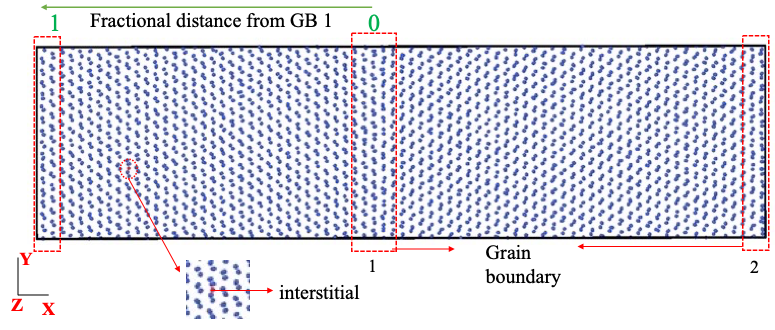
\includegraphics[width = 0.7\textwidth]{Picture1.png}}%%%
\DIFdelendFL \DIFaddbeginFL \subfloat[]{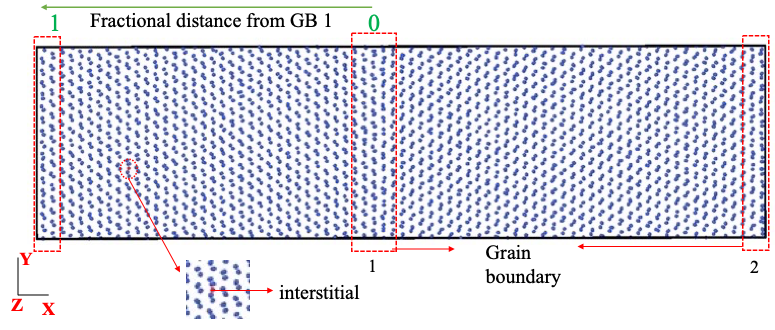
\includegraphics[width = 0.7\textwidth]{1_Picture1.png}}\DIFaddendFL \\
\caption{A snapshot of the simulation box which consists of two grain boundaries (GB1 and GB2) and an interstitial. GB1 and GB2 are the same grain boundary. The fractional distance is defined such that it is 0 at the GB1 core and 1 at the GB2 core.}
\label{fig:GB}
\end{figure}

Utilizing these distance-dependent formation energies, the segregation energy ($E_{\mathrm{s}}$) and the interaction length ($l_{\mathrm{int}}$) are calculated. $E_{\mathrm{s}}$ is defined as:

\begin{equation}
\label{eq:eform2}
E_{\mathrm{s}}(r)_{\mathrm{i/v}} = \DIFdelbegin \DIFdel{E}\DIFdelend \DIFaddbegin \DIFadd{-E}\DIFaddend _{\mathrm{f}}(r)_{\mathrm{i/v}} \DIFdelbegin \DIFdel{- }\DIFdelend \DIFaddbegin \DIFadd{+ }\DIFaddend E_{f,i/v}^{bulk}
\end{equation}

\noindent where $E_{f}^{bulk}$ is the formation energy of a point defect in the bulk $\alpha$-U system and $E_f(r)_{i/v}$ is the formation energy of a defect in a bi-crystal $\alpha$-U system at a distance $r$ from the GB. In this formulation, a positive $E_{\mathrm{s}}$ indicates an attraction of the point defect to the GB, while a negative $E_{\mathrm{s}}$ indicates that it is thermodynamically unfavorable to form a point defect adjacent to the grain boundary. The  $l_{\mathrm{int}}$ is the length at which the $E_{\mathrm{s}}(r)$ becomes zero, indicating that there is no interaction between the defect and the GB.  

\subsection{Diffusion in Grain Boundaries}\label{sec:comp2}
\par Self-diffusion along grain boundaries is calculated via MD simulations 
%utilizing the differential method (\Cref{eq:ein}). In order to perform this method, 
by relaxing a grain boundary in an NPT ensemble as described in \cref{sec:comp1}. This relaxed structure is further evolved by keeping the volume fixed for 3~ns to 5.5~ns, depending on the temperature of interest, with higher temperatures using shorter relaxation times. During these diffusion calculations, the Nos\'{e}-Hoover thermostat is implemented to mitigate the impact of switching from an NPT to an NVT ensemble. Due to the implementation of the Langevin thermostat, converting from an NPT to an NVT ensemble generates some residual stress within the system which is avoided via the exclusive use of the Nos\'{e}-Hoover thermostat/barostat. The differences in thermostat/barostat should make no difference in the actual simulation behavior, but this distinction is included here for completeness. 

The mean squared displacement (MSD) of the atoms around the GB (considering a spatial bin centered at the GB in the middle of the simulation box) is calculated as a function of time to obtain diffusion coefficients. To obtain statistically significant results, six different simulations are performed at each temperature. The number of atoms in the diffusivity simulations varies between 6,000 to 10,000 depending on the GB type. The GB area varies between 700 - 1300 {\AA${^2}$}. The GB spatial bin thickness ($l_{\mathrm{sb}}$) is related to the GB structure (structural width of GB \cite{keblinski1999self} obtained from the common neighbor analysis at the specific temperature) and valued as 16 {\AA} to 20 {\AA}. The MSD is only recorded for atoms within a thickness of $l_{\mathrm{sb}}$ related to the GB structure and denoted by $MSD_{\mathrm{sb}}$. After the simulations, the GB MSD is modified via the inclusion of the GB thickness (\DIFdelbegin \DIFdel{$l_{\mathrm{GB}}$}\DIFdelend \DIFaddbegin \DIFadd{$\delta$}\DIFaddend ) as in \Cref{eq:dim} \cite{USi_diffusion}, 
%
\begin{equation}
\label{eq:dim}
MSD_{\mathrm{GB}} =\frac{l_{\mathrm{sb}}}{\delta} \times MSD_{\mathrm{sb}}
\end{equation}
%
identifying the $\delta$ from the atomic trajectories showing the atoms move at least one nearest neighbor distance (obtained from OVITO \cite{ovito}) of the atoms within the spatial bin. The underlying assumption of this equation is that the GB area and atomic volume remains same within the $l_{\mathrm{sb}}$ and $\delta$ lengths. When the simulation is run for sufficient time (3~ns - 5.5~ns in this work), atoms within the structural width of the GB contribute to the diffusion process \cite{keblinski1999self}, so that the constant atomic volume assumption is valid. To omit the ballistic time period of atom movement, the first 5 ps of the MSD are neglected. For some of the GBs, especially those with a lower $E_{\mathrm{gb}}$, an additional interstitial needs to be inserted to yield diffusive behaviors. The effect of the presence of additional point defects on grain boundary diffusion is also explored. In this case, either an interstitial or a vacancy is inserted within the GB interaction zone and the MSD is calculated.

\par The slope of the MSD versus time is incorporated into Einstein's relationship (\Cref{eq:ein}) to calculate the diffusion coefficient at a specific temperature,

\begin{equation}
\label{eq:ein}
D_{\mathrm{GB}} = \frac{MSD_{\mathrm{GB}}}{2dt}
\end{equation}

\noindent where $d$ is the dimensionality of the diffusion. The degree of dimensionality of diffusion is dependent upon the specific GB of interest. Finally, diffusivity is plotted as a function of inverse temperature to fit an Arrhenius relationship. 

Above 750 K, this interatomic potential predicts that grain boundaries begin to induce a phase transformation to the BCC phase. Analysis of the radial distribution function, in addition to structure analysis tools, provided evidence of this phase transformation. Thus, our study is constrained to a maximum temperature of 750 K. 


\FloatBarrier
\section{Results}

In this section, findings from the current work on point defect interaction with grain boundary and grain boundary self-diffusion is described in two separate subsections as a function of temperature and defect (both point defect and grain boundary) types. Finally the Coble creep rate is calculated within the studied temperature range.

\subsection{Point Defect Interactions with Grain Boundaries}

In this section, the interaction of an interstitial and a vacancy with six different grain boundaries of $\alpha$-U is described within a temperature range of 300 K to 600 K. \Cref{fig:Seg_inter_500,fig:Seg_vacancy_500} represent the formation energies of an interstitial and a vacancy plotted as a function of the fractional distance from a GB core at 500 K. Results for the other studied temperatures (300 K, 400 K, and 600 K) are shown in \Cref{fig:Seg_inter,fig:Seg_vacancy} in the appendix. The $E_{\mathrm{f}}$ in these figures are the average $E_{\mathrm{f}}$ of the point defect at that specific distance, and the fractional distance from the GB is shown up to 0.6, which fully encompasses the extension into the bulk. There is a common trend among the plots, in that each shows a smaller value of the $E_{\mathrm{f}}$ near the GB, followed by an increase in the $E_{\mathrm{f}}$ until reaching a constant value at a sufficient distance from the GB. How much the $E_{\mathrm{f}}$ of a given point defect is decreased due to the presence of a GB at a specific temperature depends on the GB type (orientation) and energy, as well as the defect type. For instance, the coherent twin GBs (A1 and C1) have a negligible effect on the vacancy $E_{\mathrm{f}}$ (see \Cref{fig:Seg_vacancy_500}a, c), but reduce the interstitial $E_{\mathrm{f}}$ (see \Cref{fig:Seg_inter_500} a,c). The higher energy grain boundaries (A2, B2, and C2) show strong interactions for both vacancies and interstitials. 

\begin{figure}[h!]
\centering
\DIFdelbeginFL %DIFDELCMD < \subfloat[]{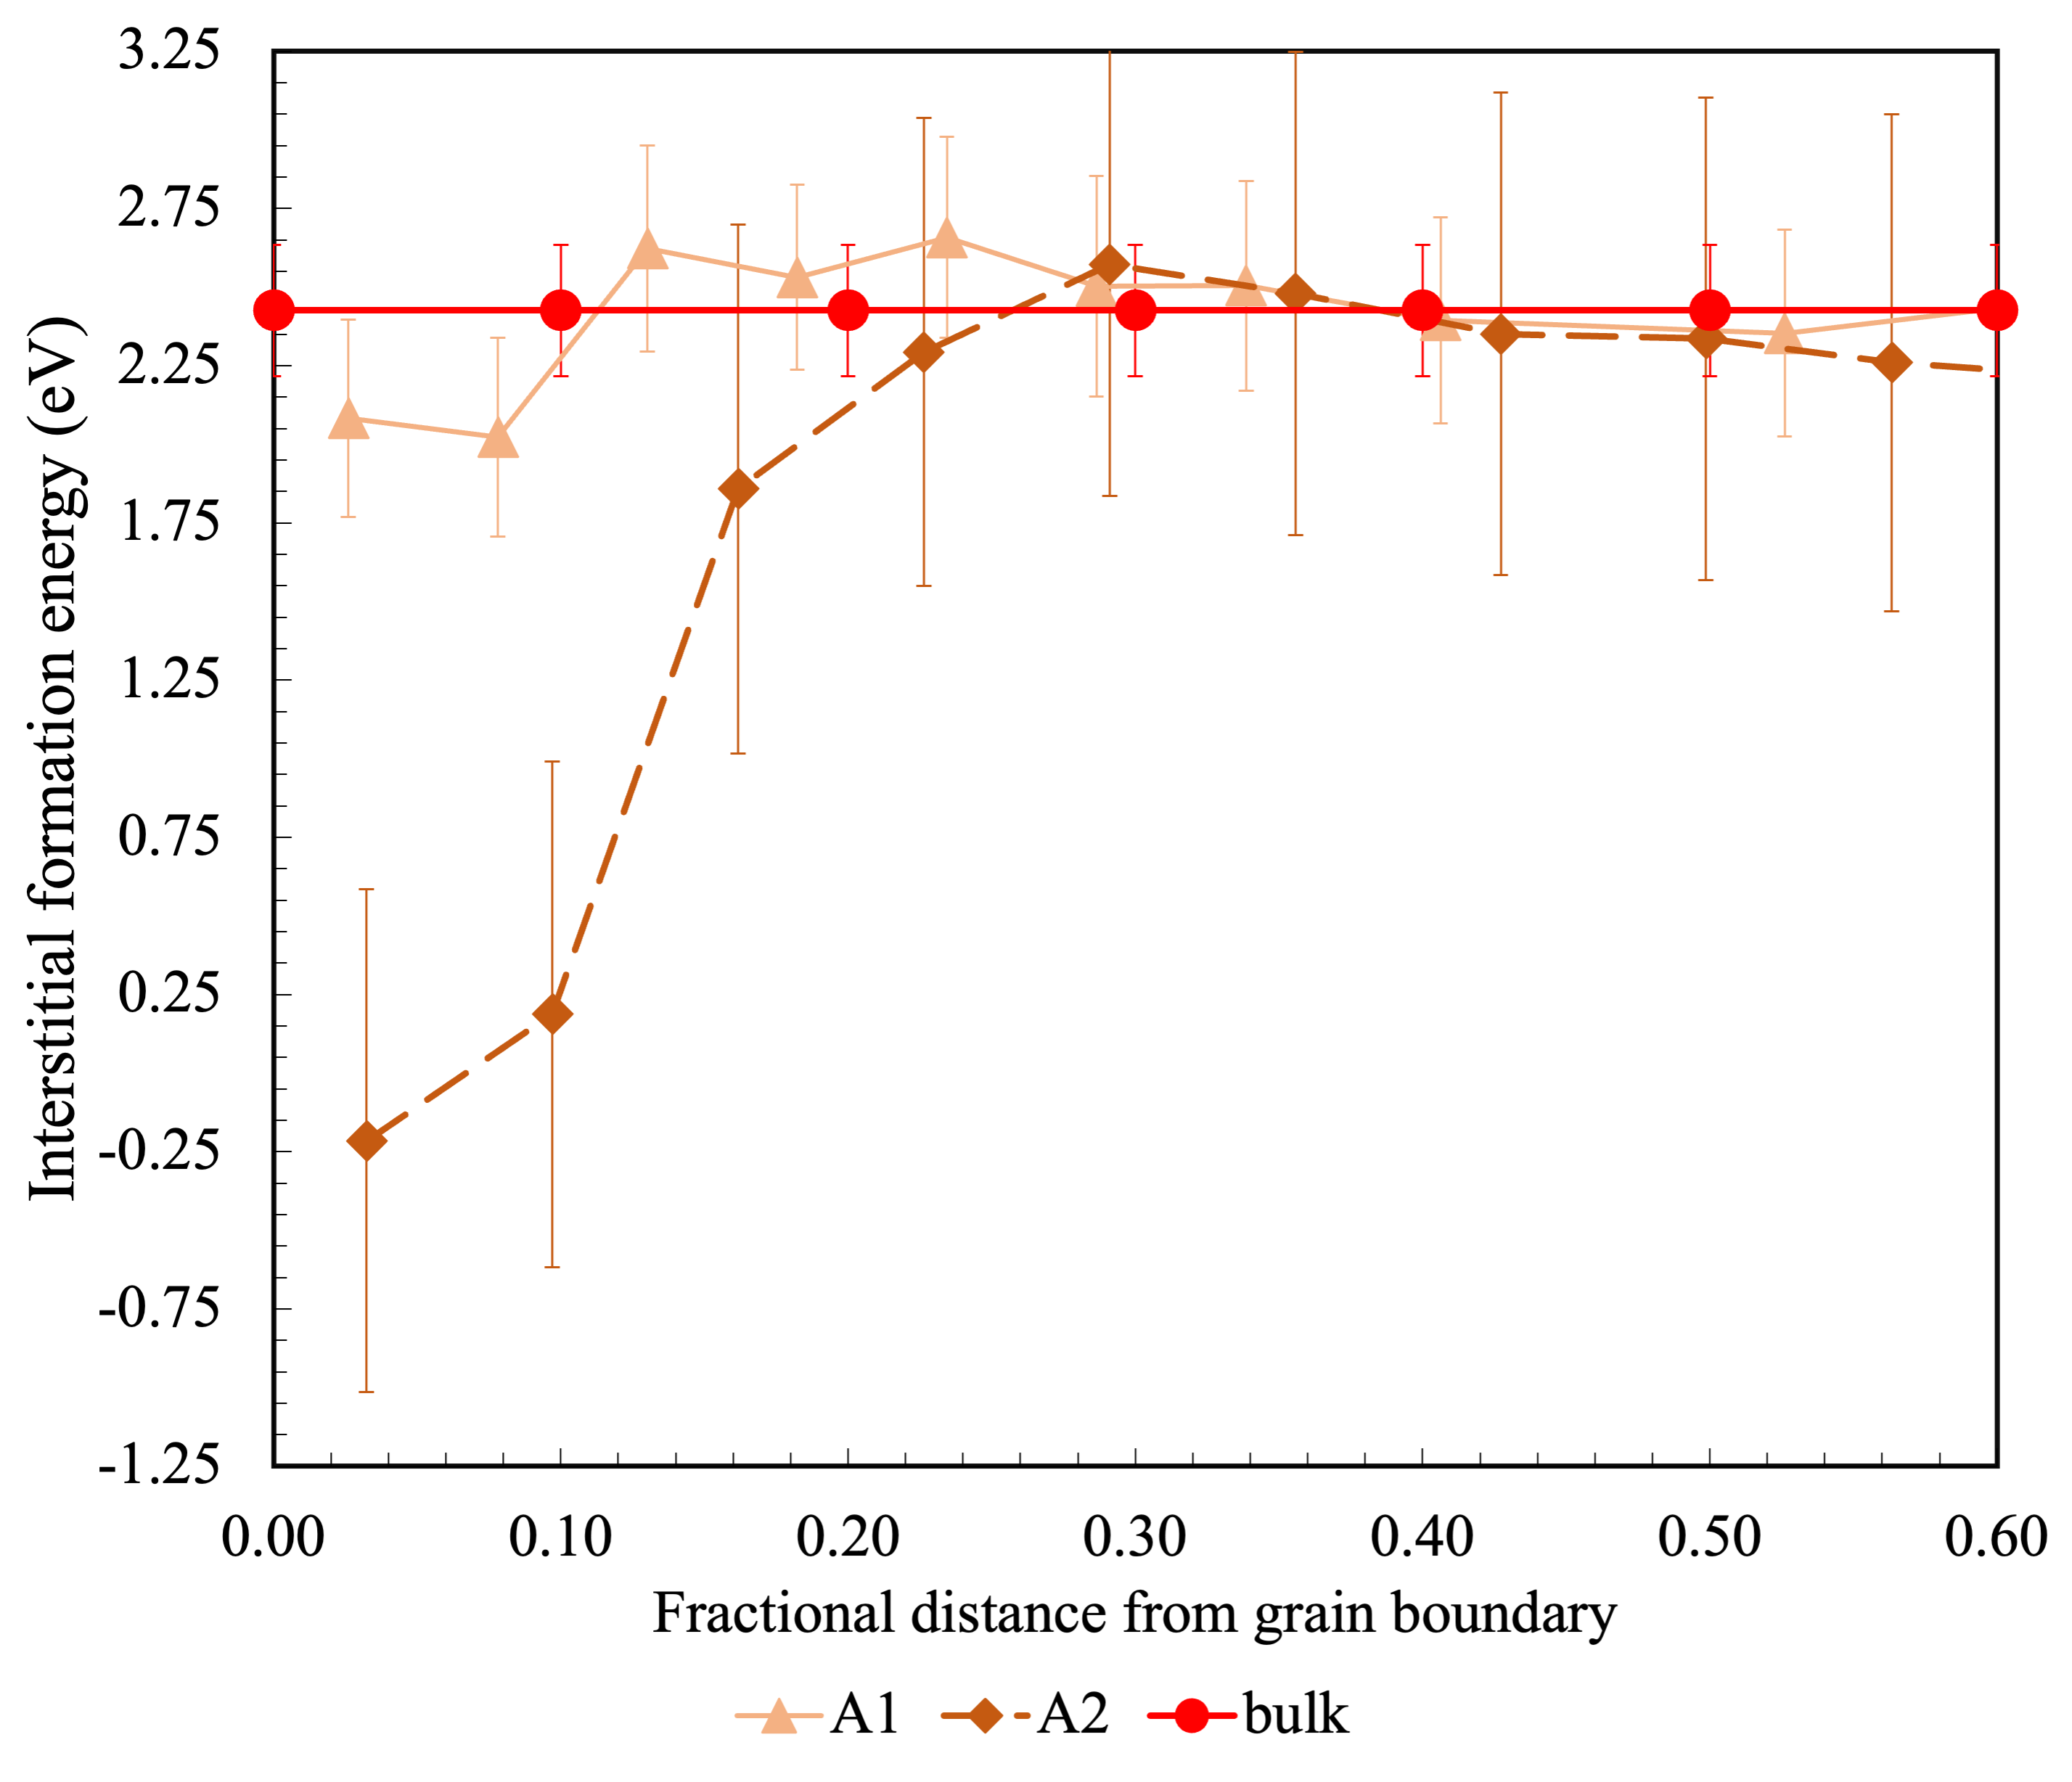
\includegraphics[width = 2.0in]{A_500_Inter.png}}
%DIFDELCMD < \subfloat[]{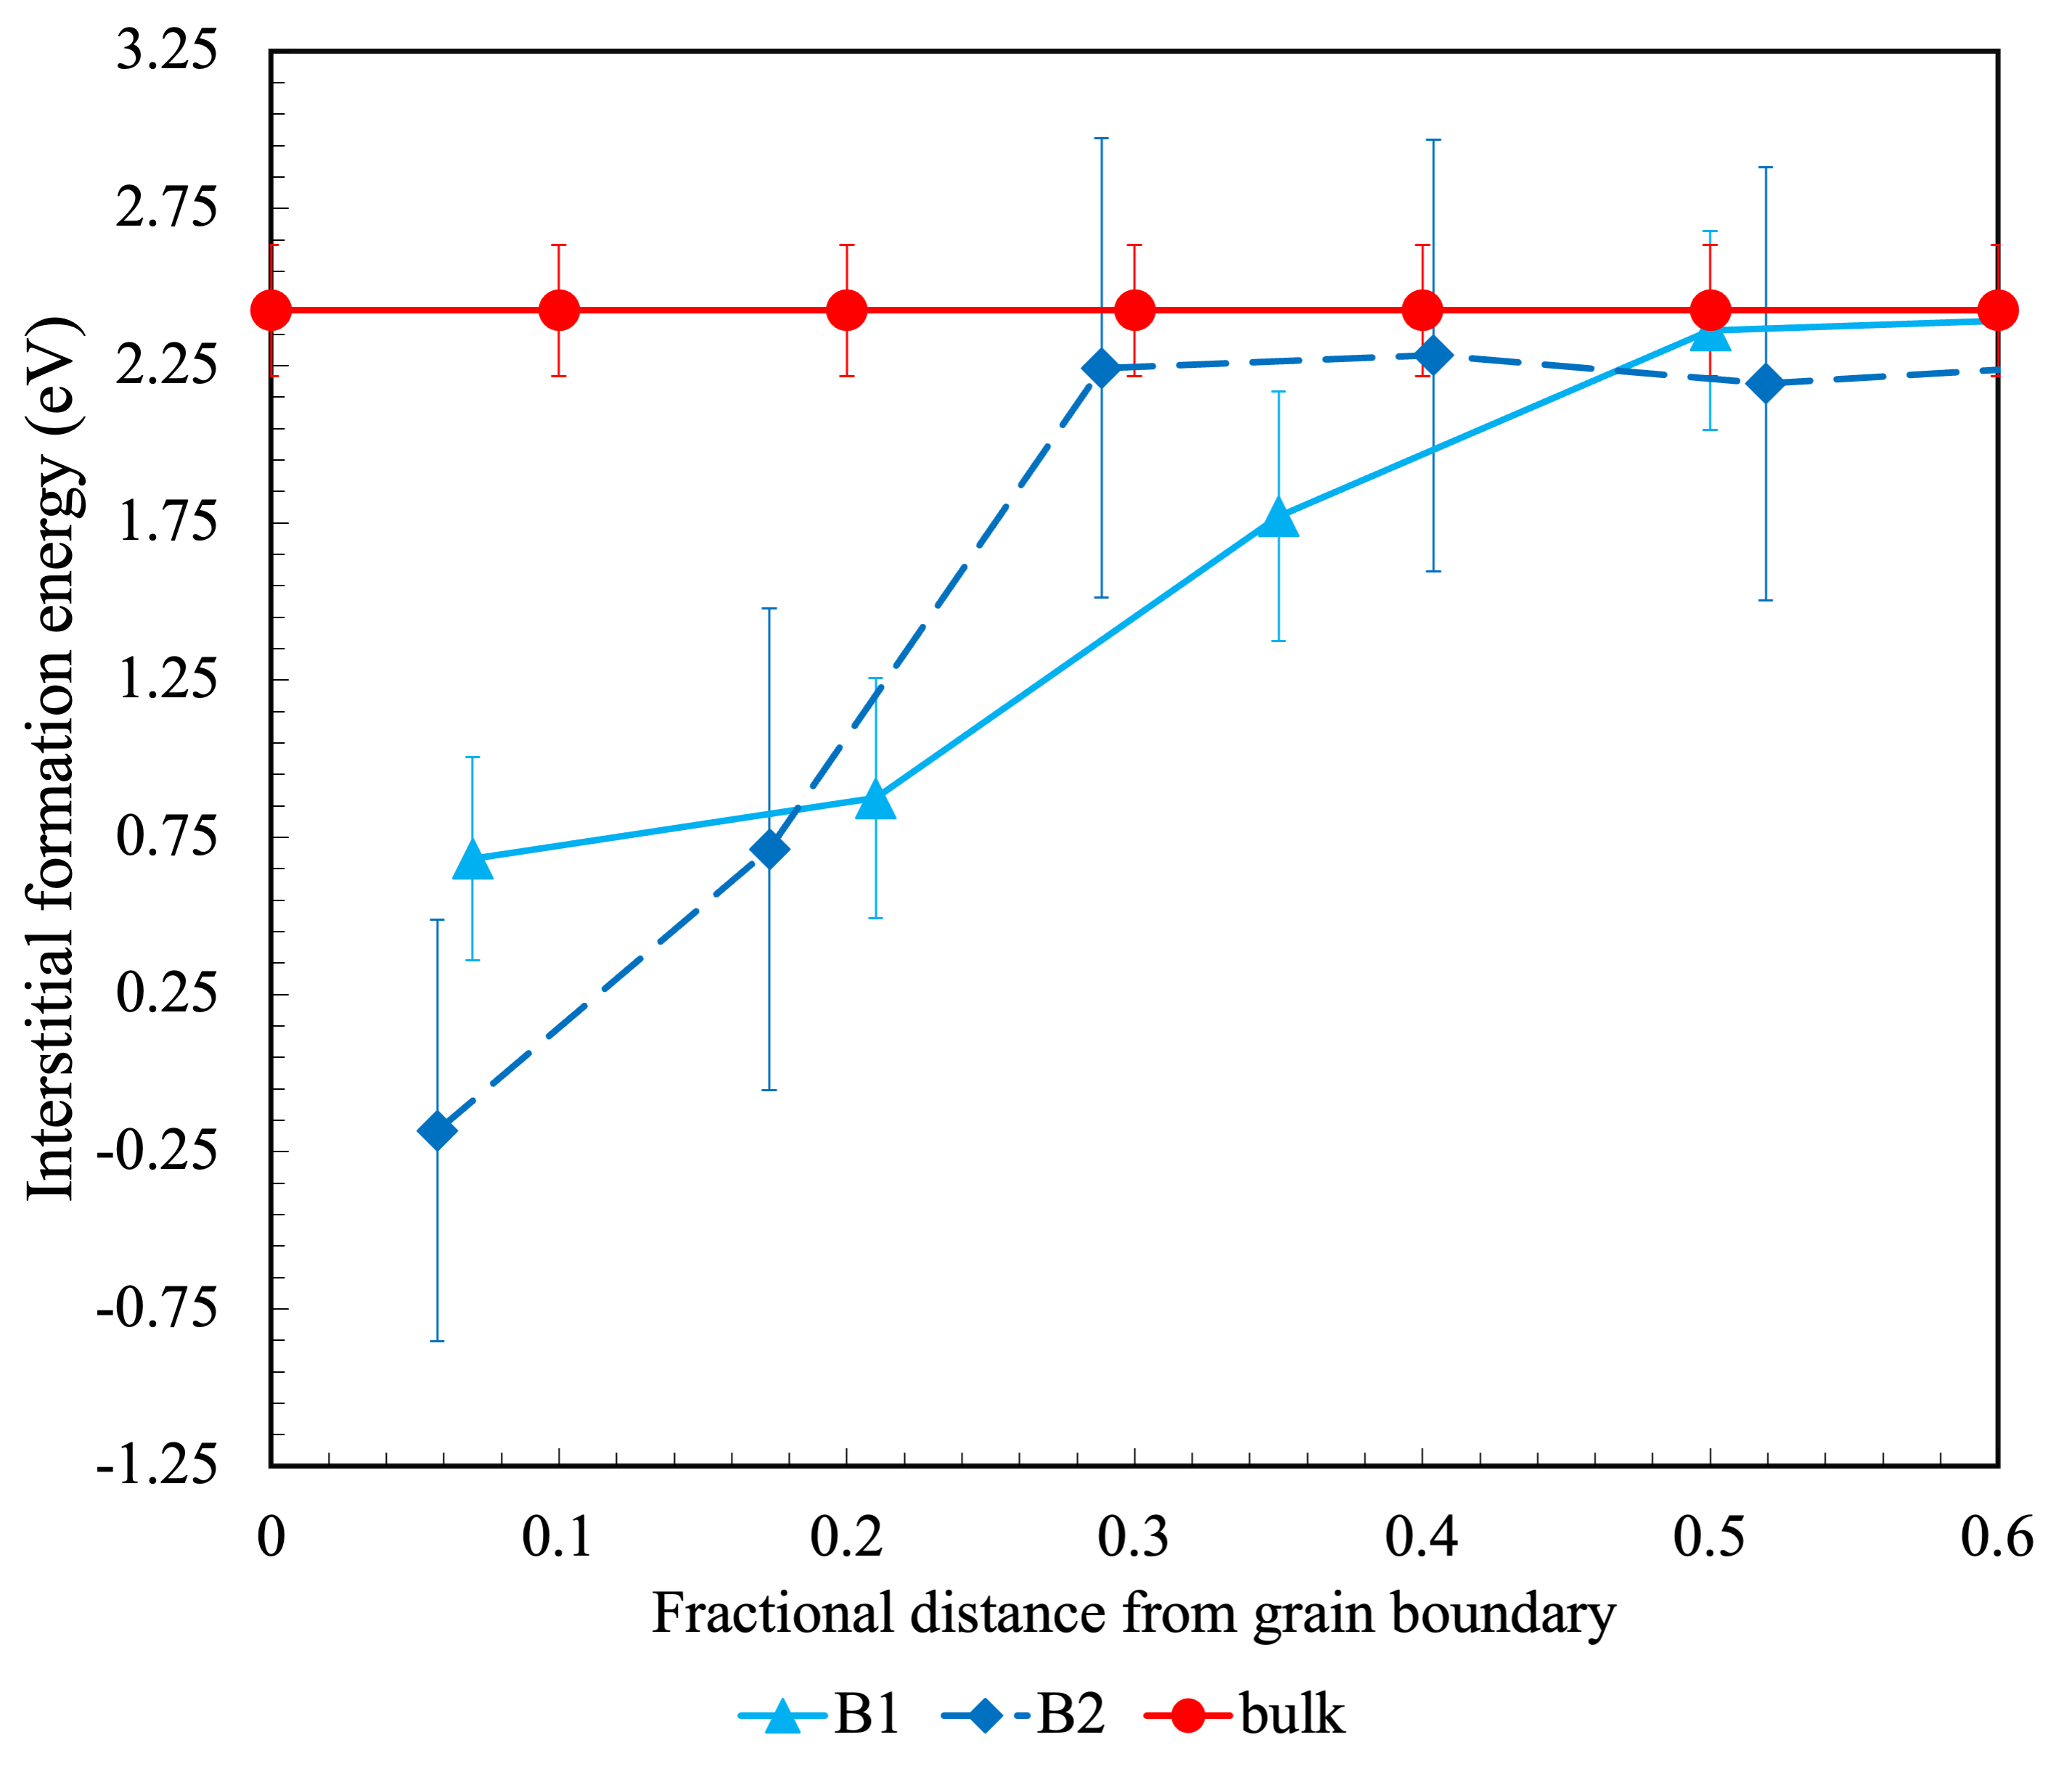
\includegraphics[width = 2.0in]{B_500_Inter.png}}
%DIFDELCMD < \subfloat[]{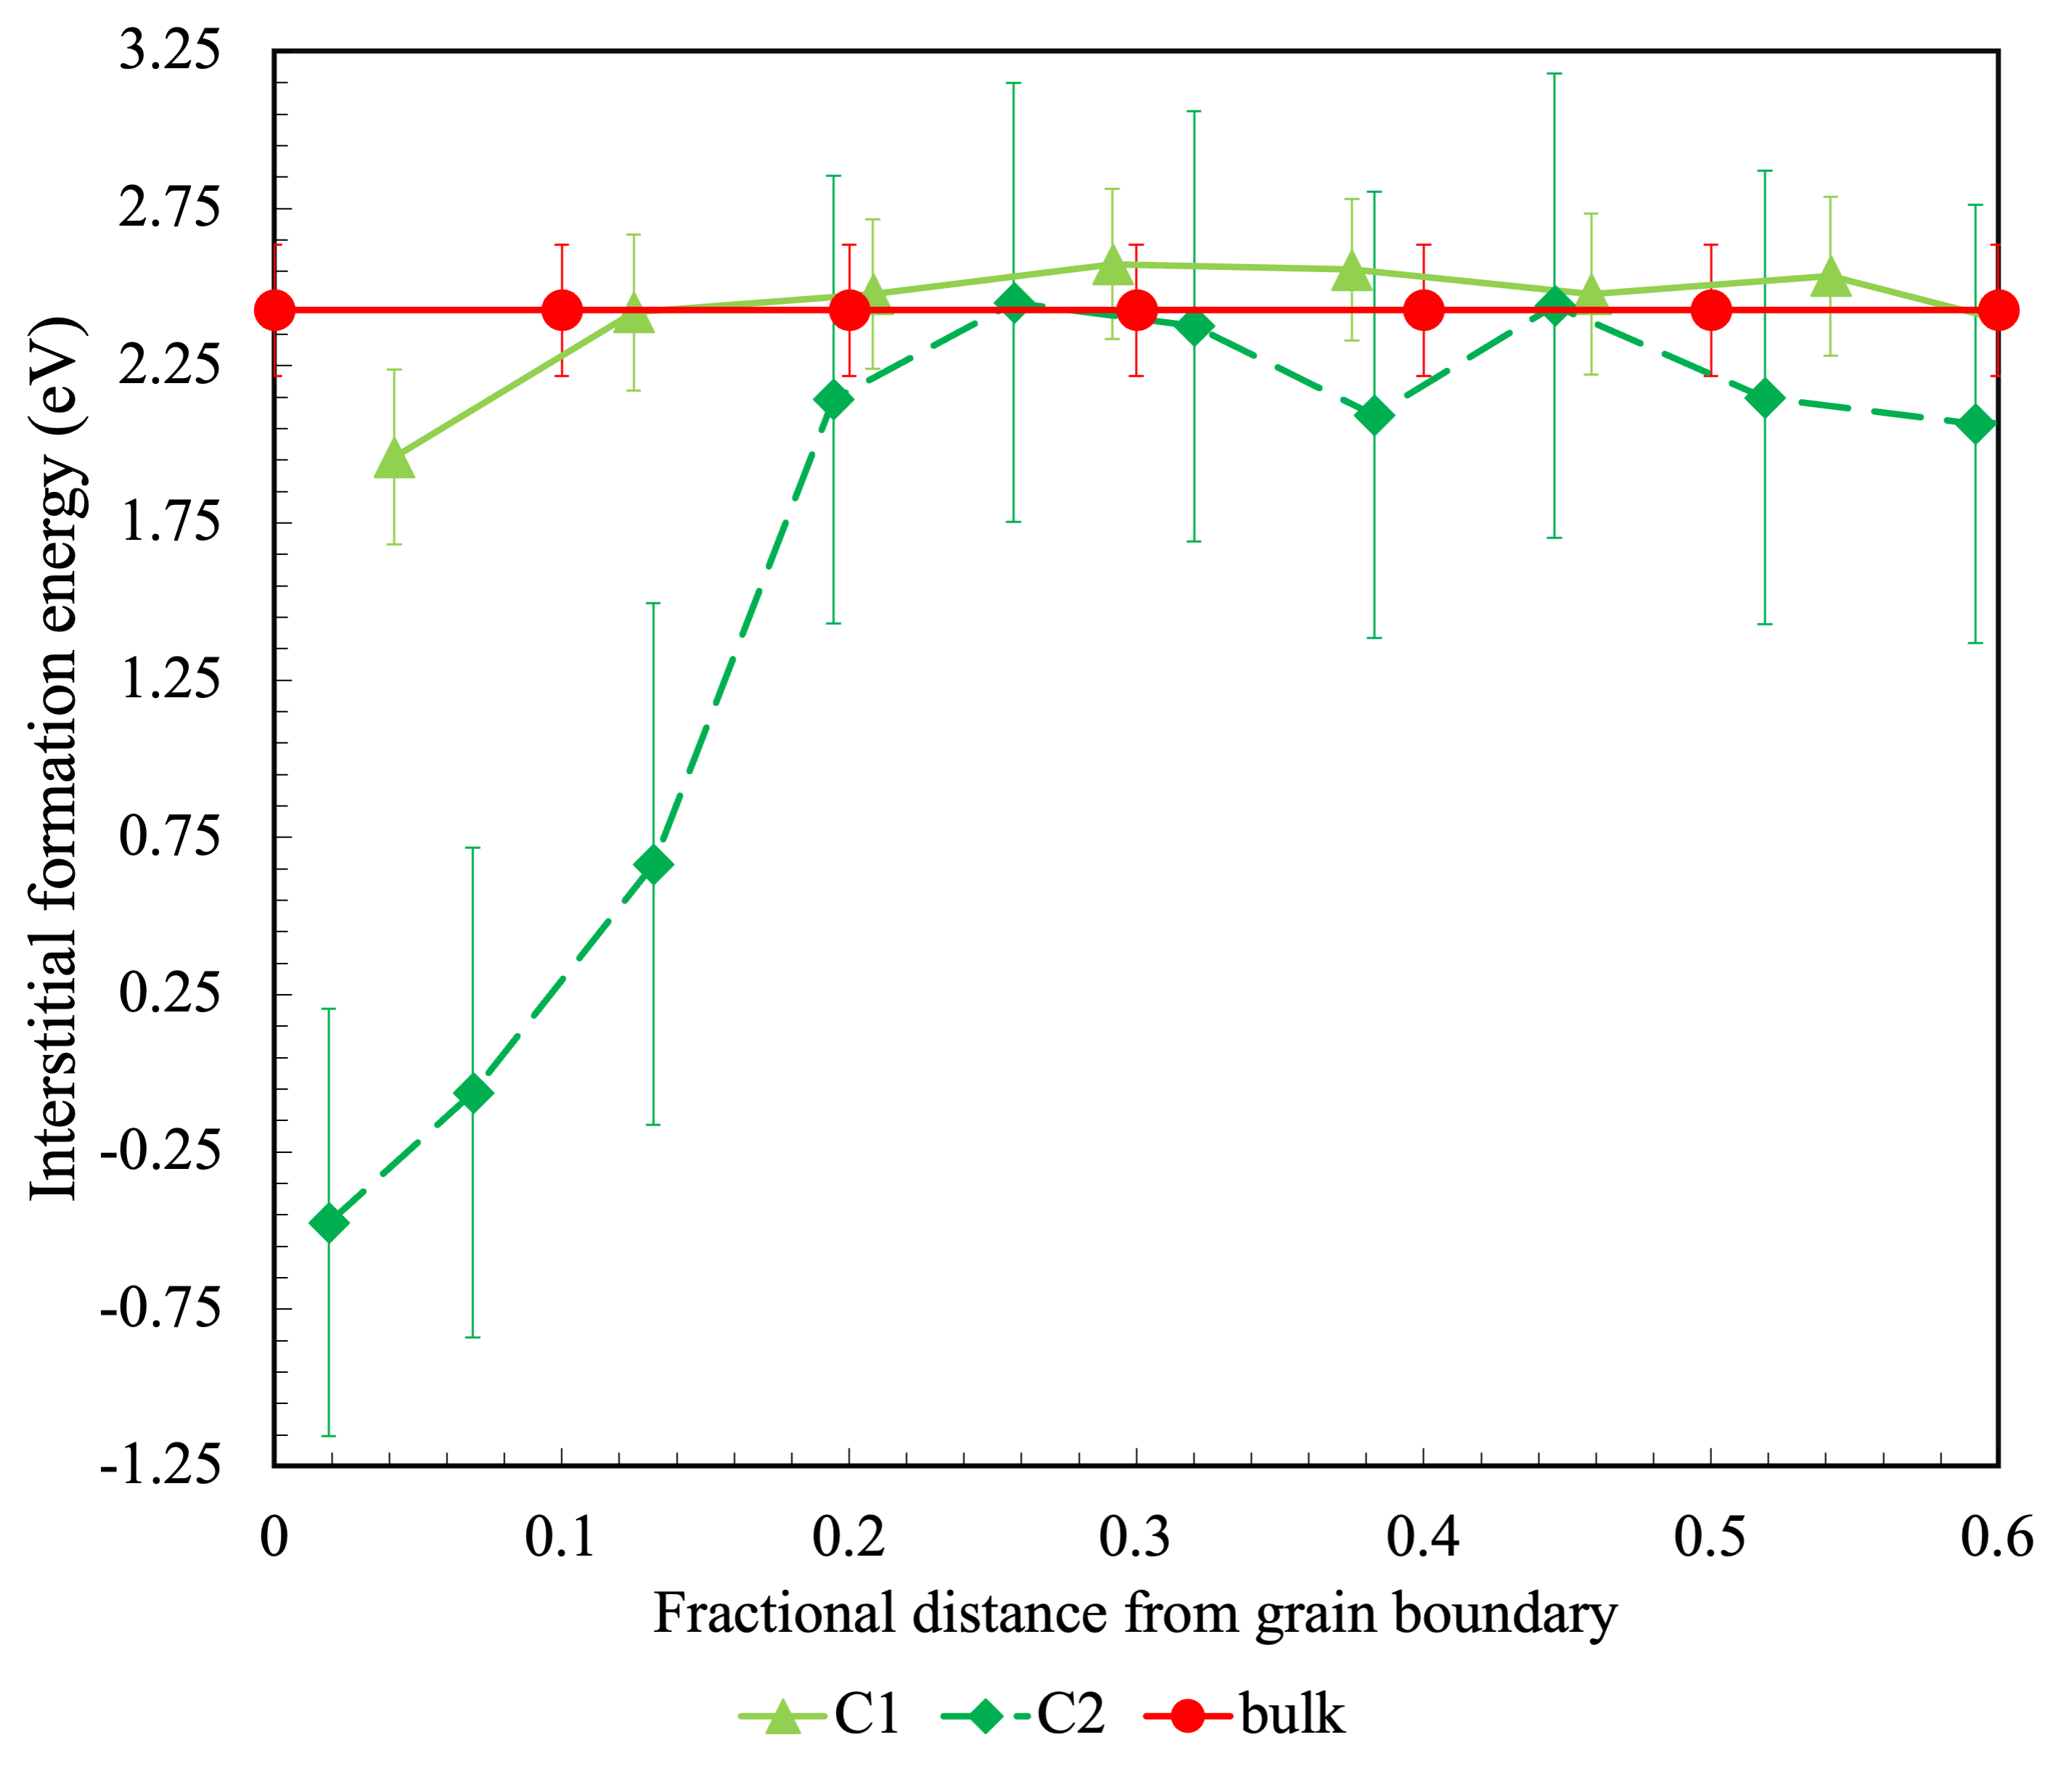
\includegraphics[width = 2.0in]{C_500_Inter.png}}
%DIFDELCMD < %%%
\DIFdelendFL \DIFaddbeginFL \subfloat[]{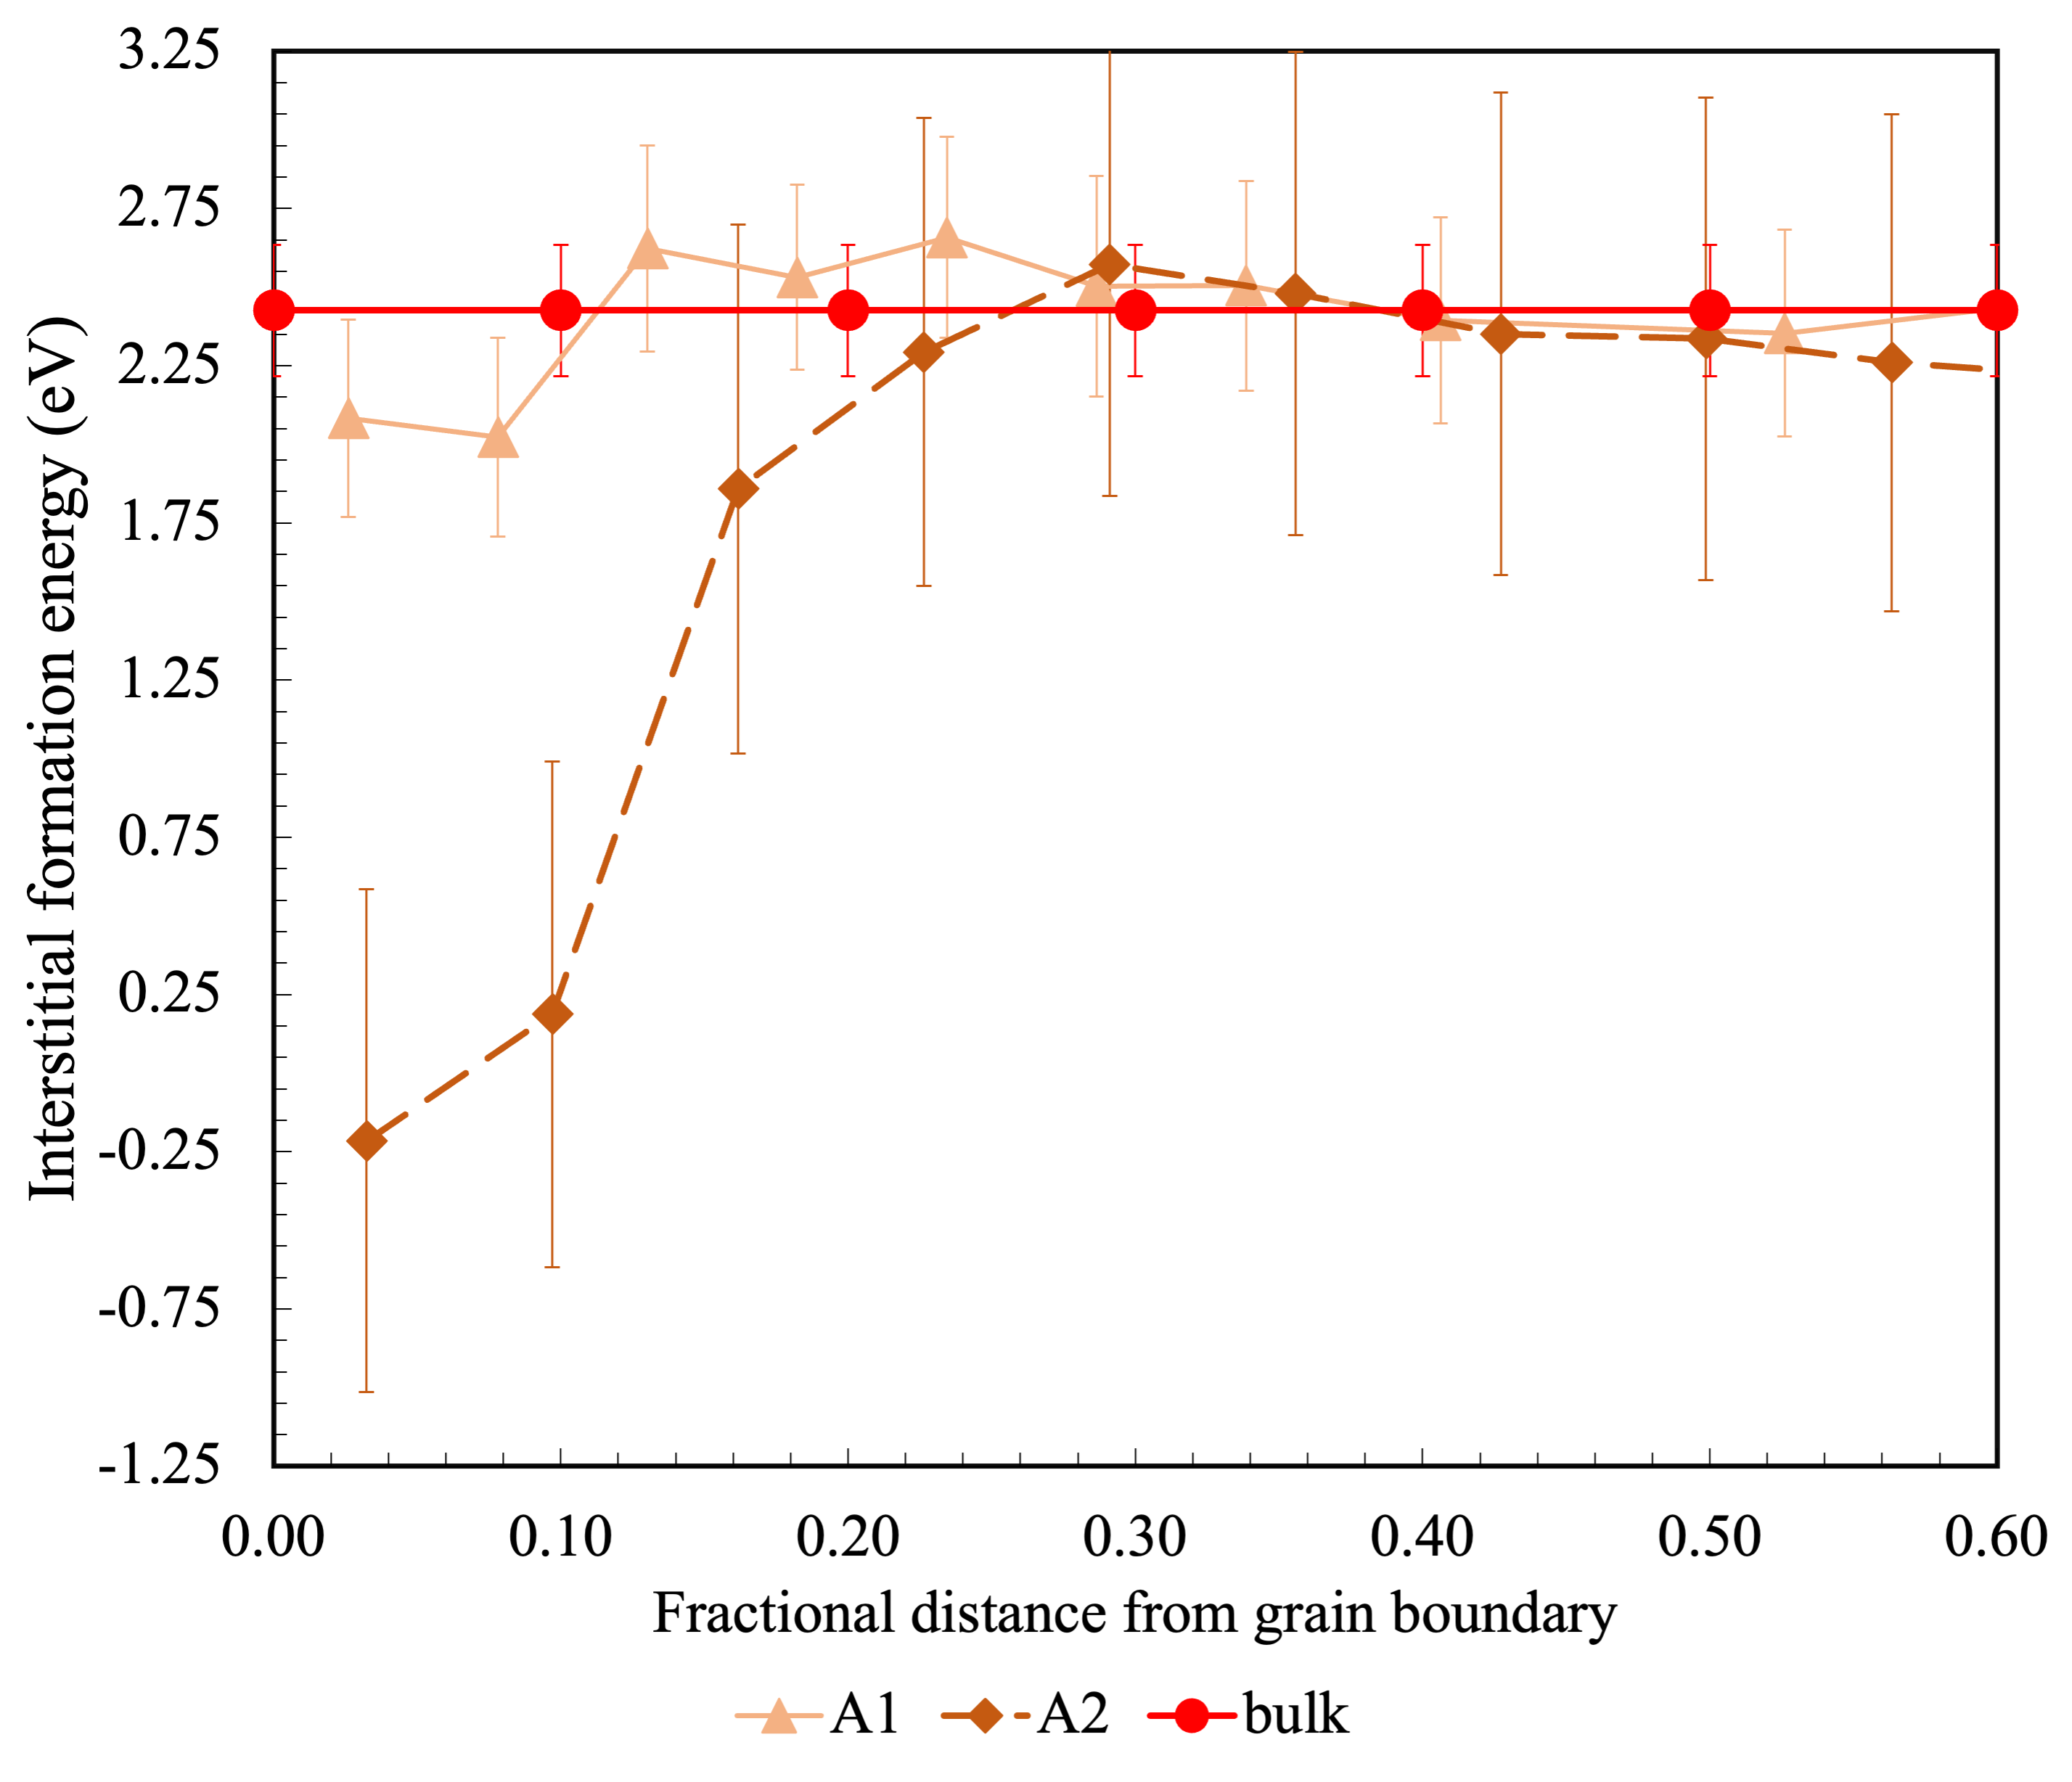
\includegraphics[width = 2.0in]{2_A_500_Inter.png}}
\subfloat[]{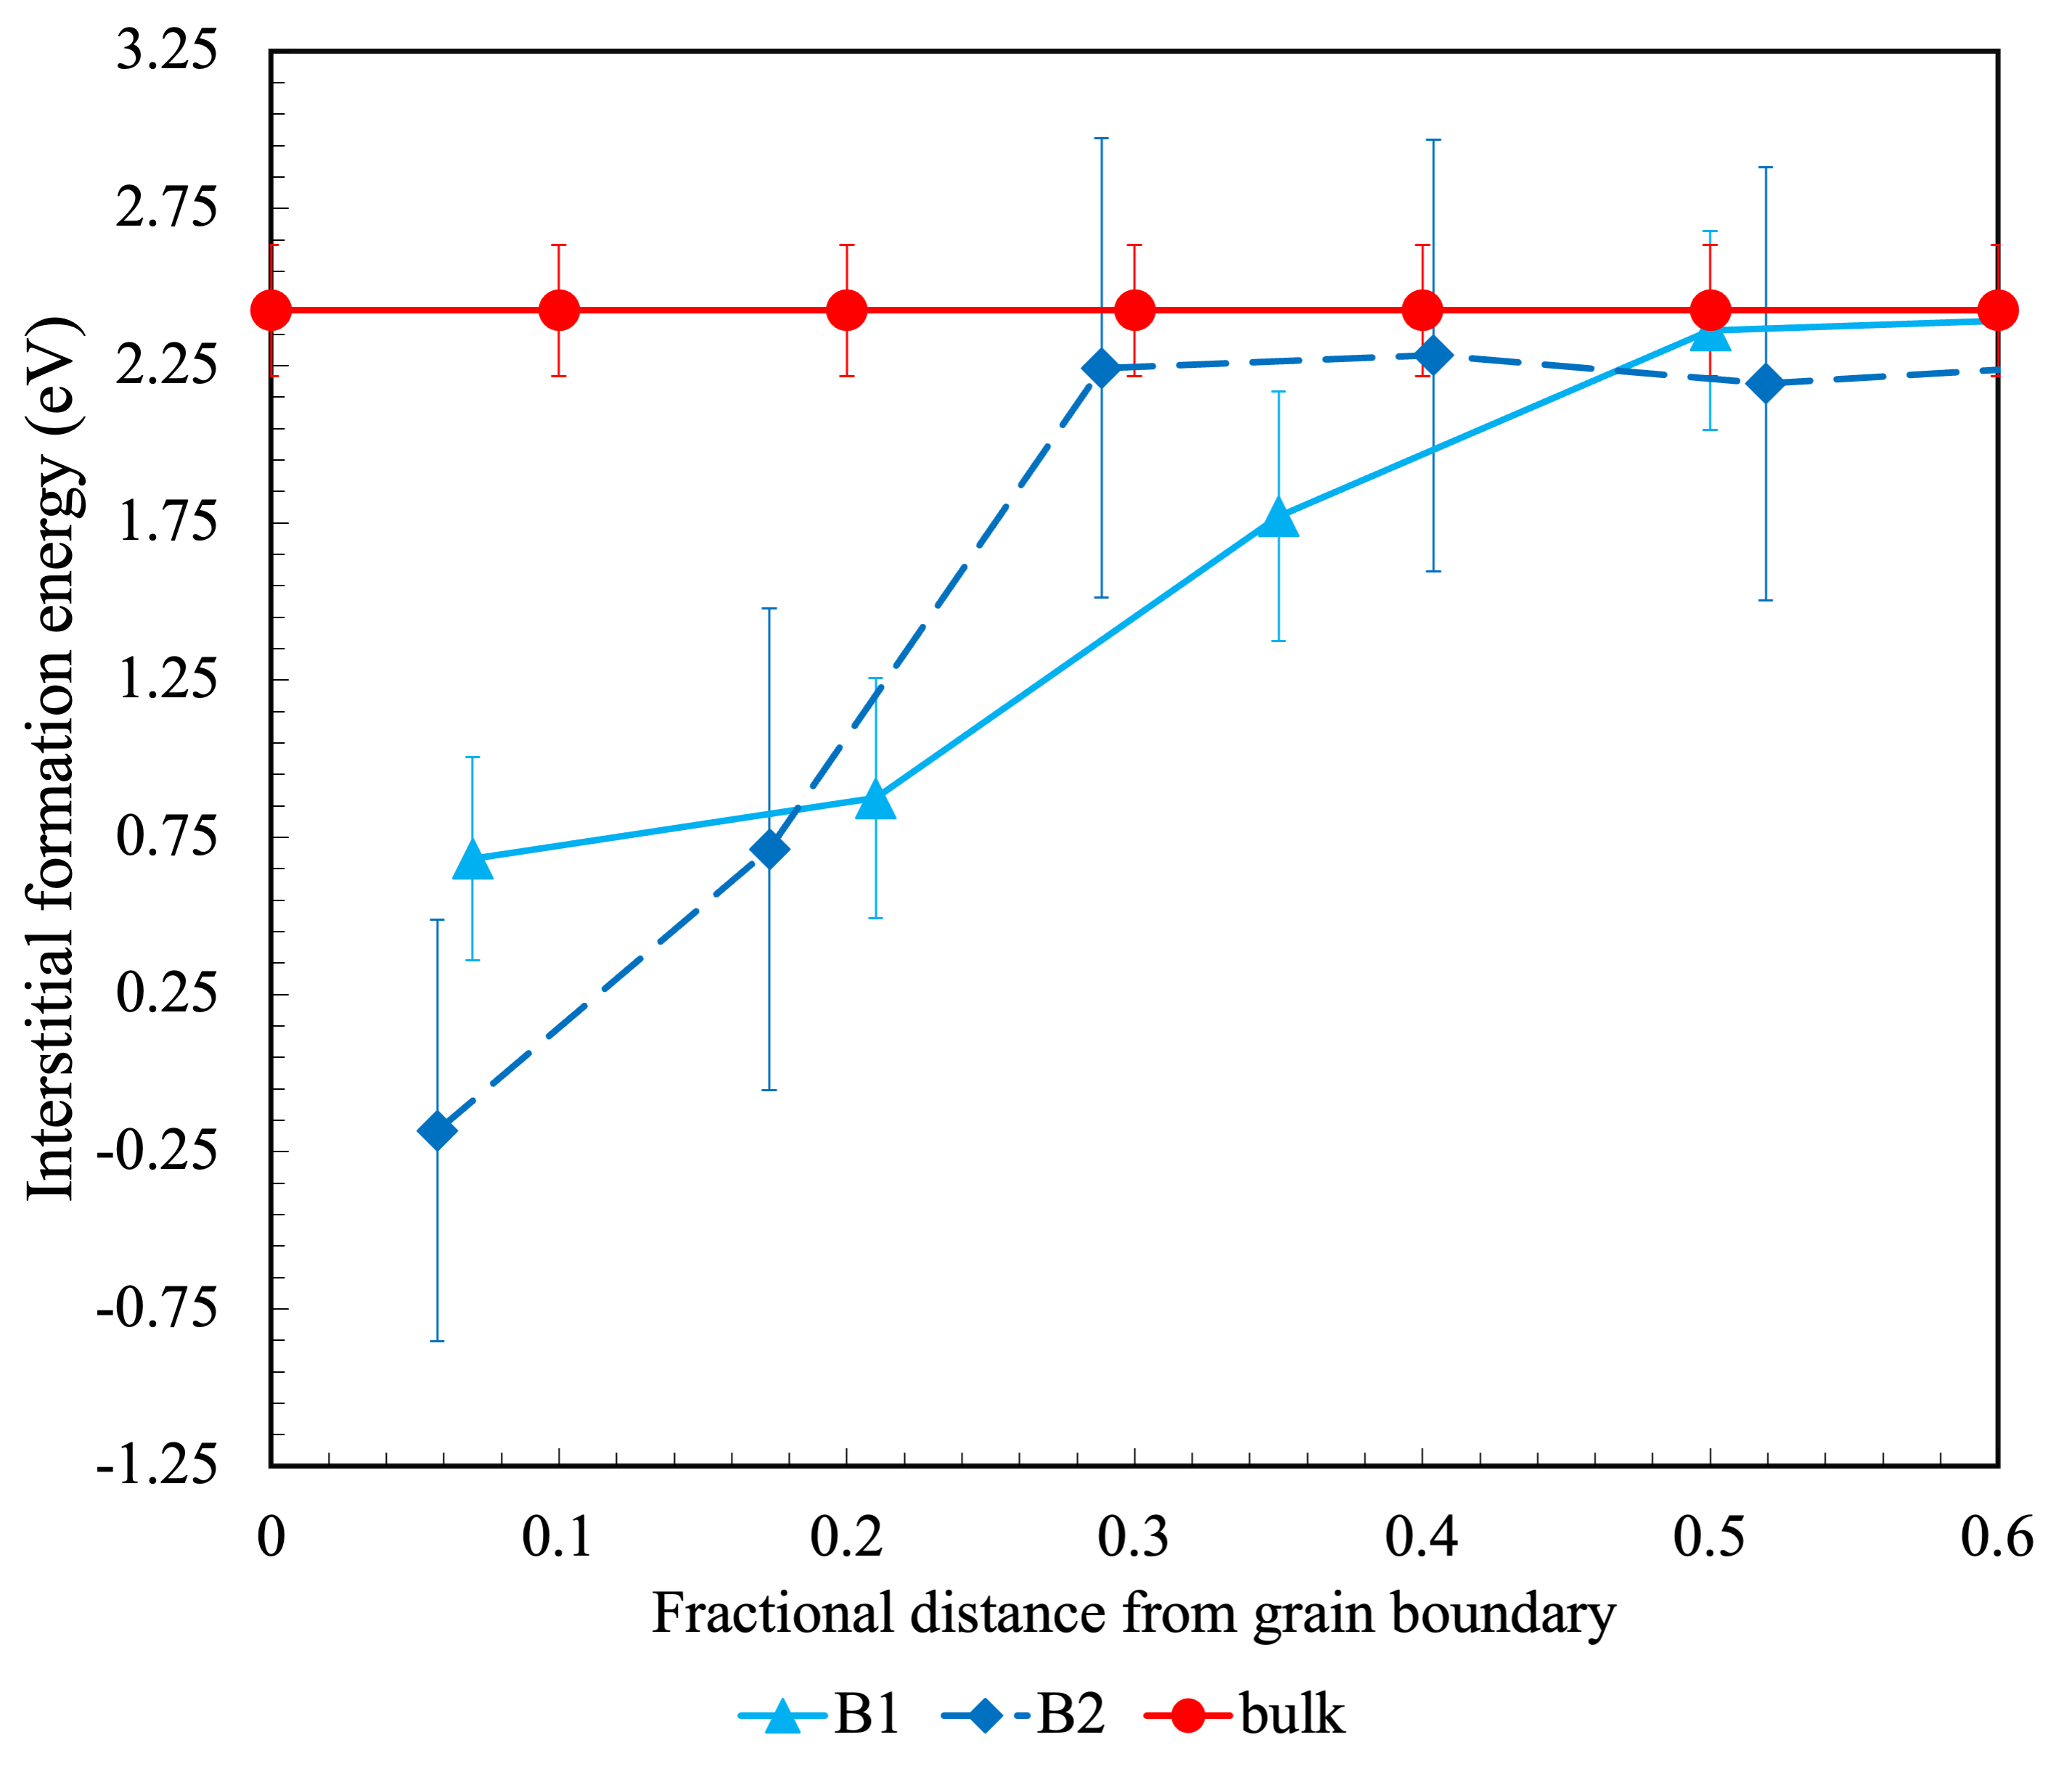
\includegraphics[width = 2.0in]{2_B_500_Inter.png}}
\subfloat[]{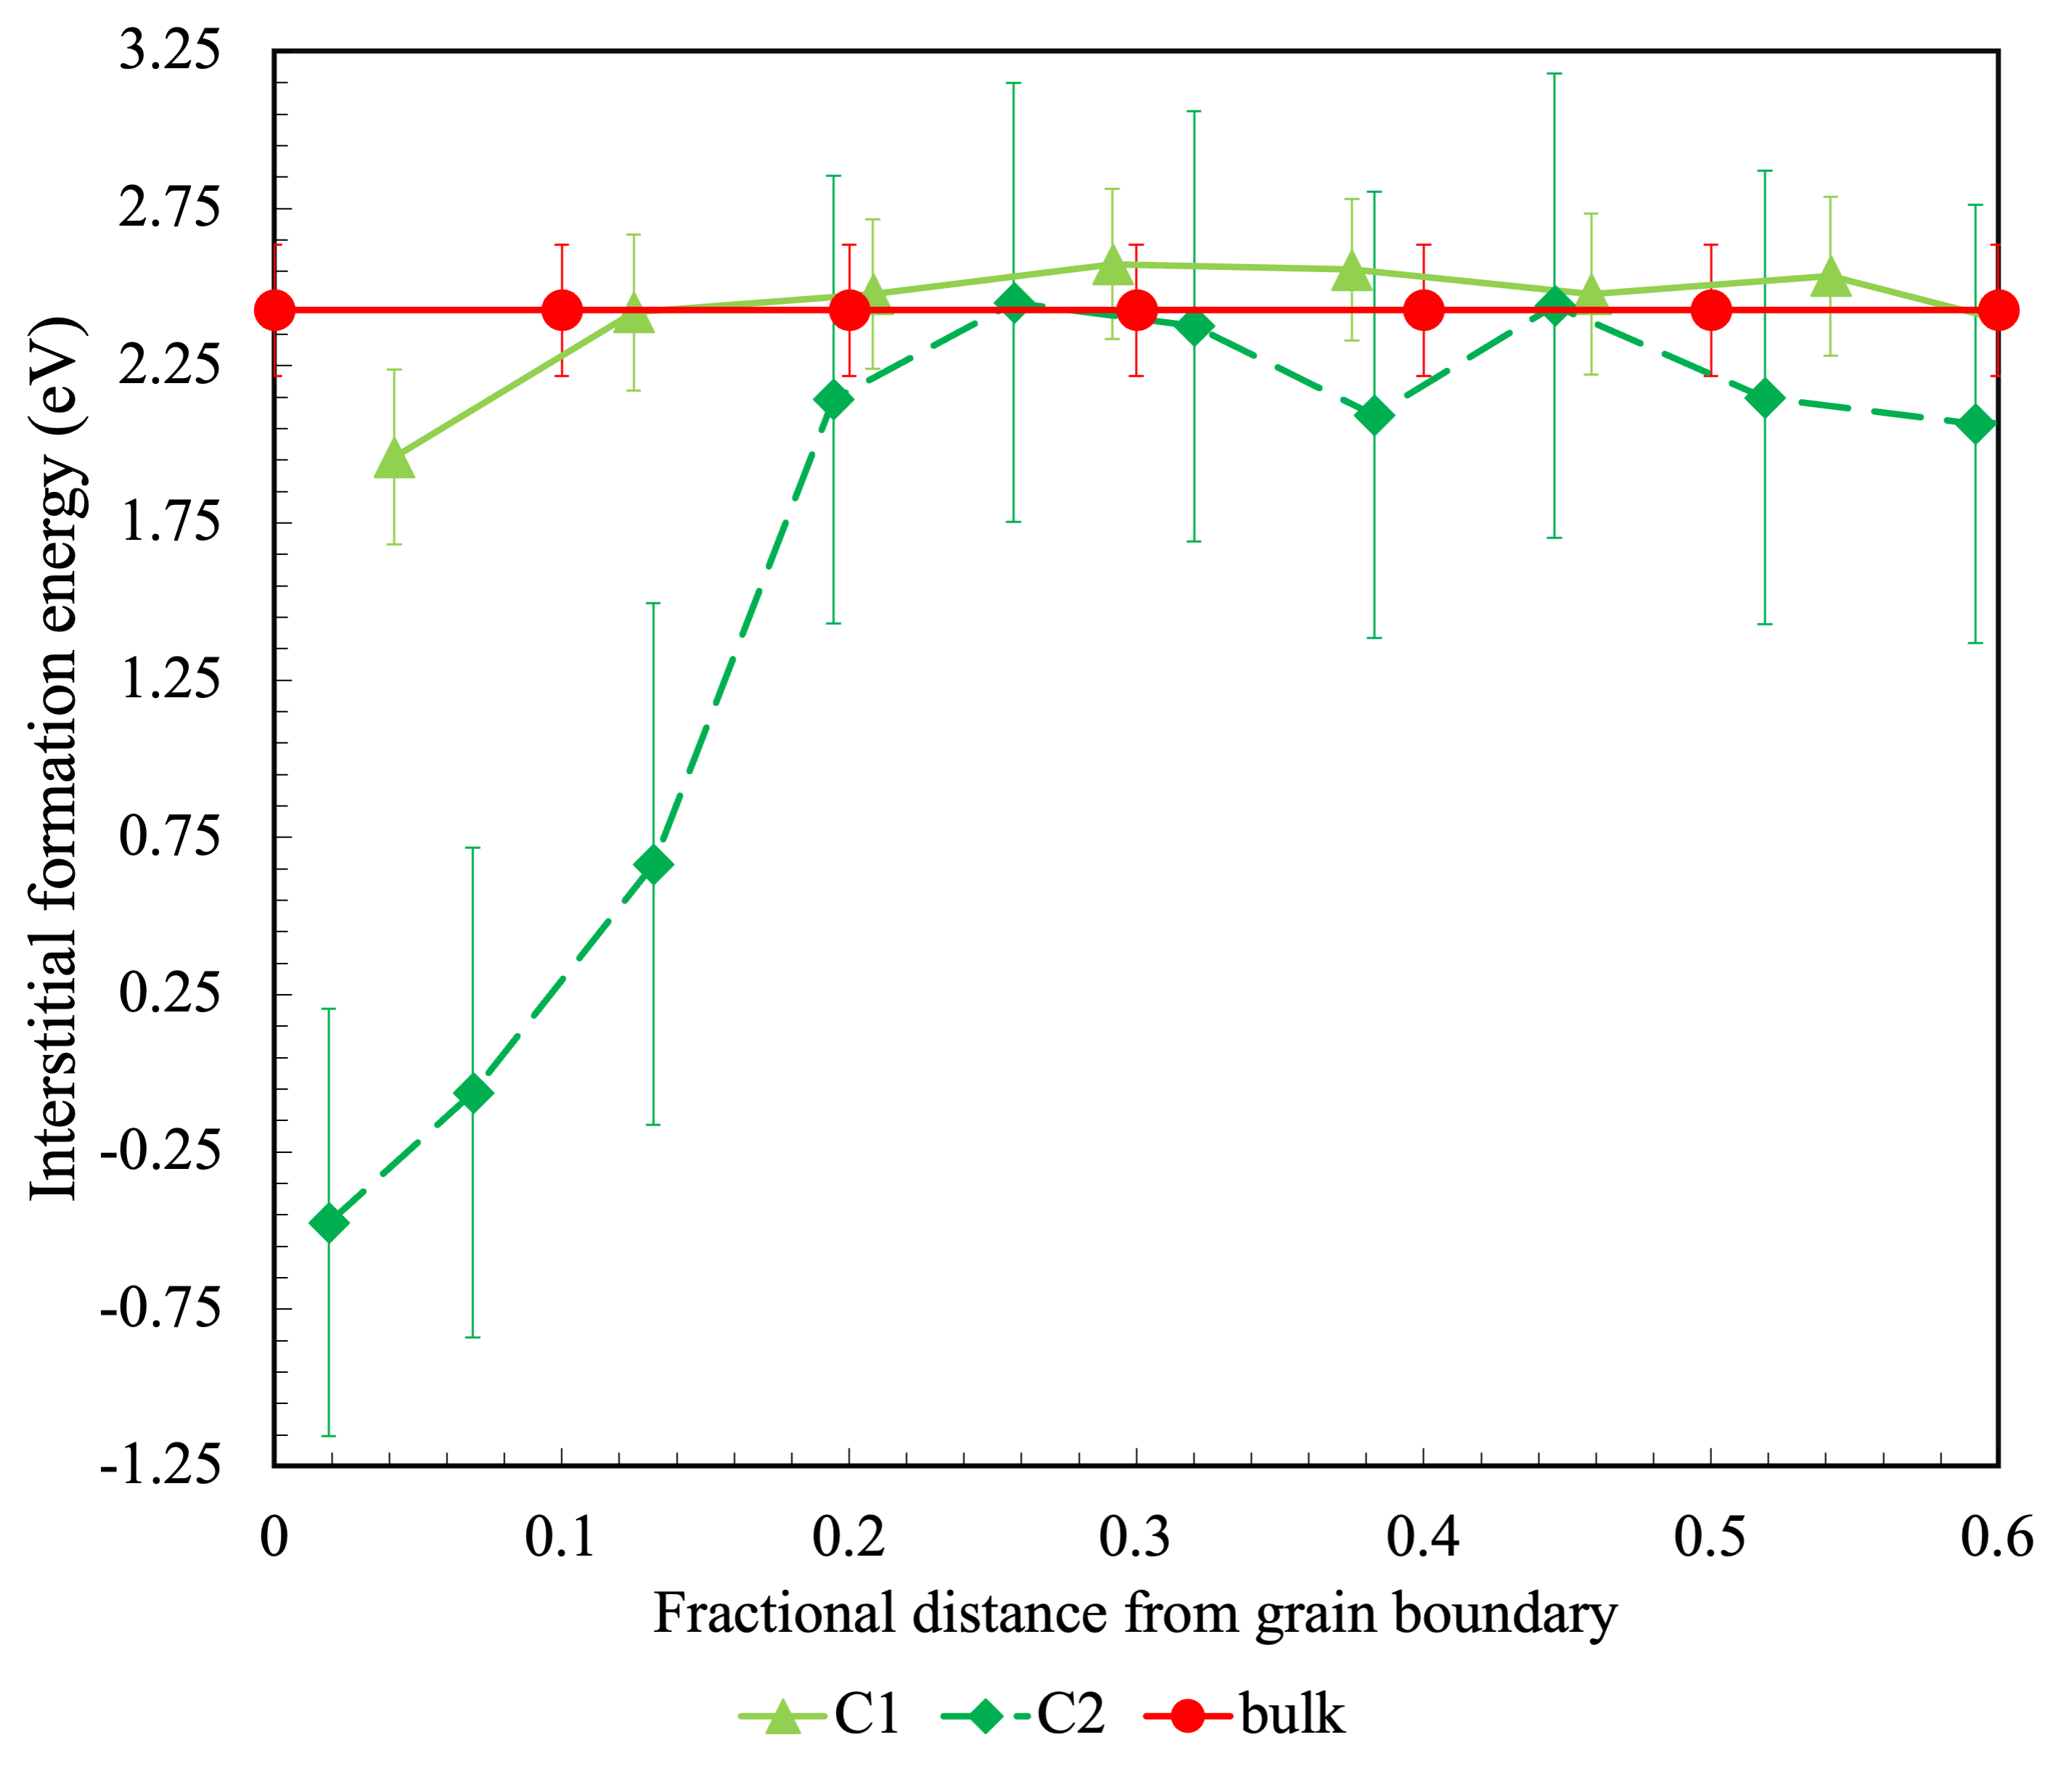
\includegraphics[width = 2.0in]{2_C_500_Inter.png}}
\DIFaddendFL \caption{Average formation energy of an interstitial at 500 K as a function of fractional distance from (a) type A, (b) type B, and (c) type C GB core. The red line shows the formation energy of an interstitial in pristine $\alpha$-U. Error bars here show twice the standard error.}
\label{fig:Seg_inter_500}
\end{figure}

\begin{figure}[h!]
\centering
\DIFdelbeginFL %DIFDELCMD < \subfloat[]{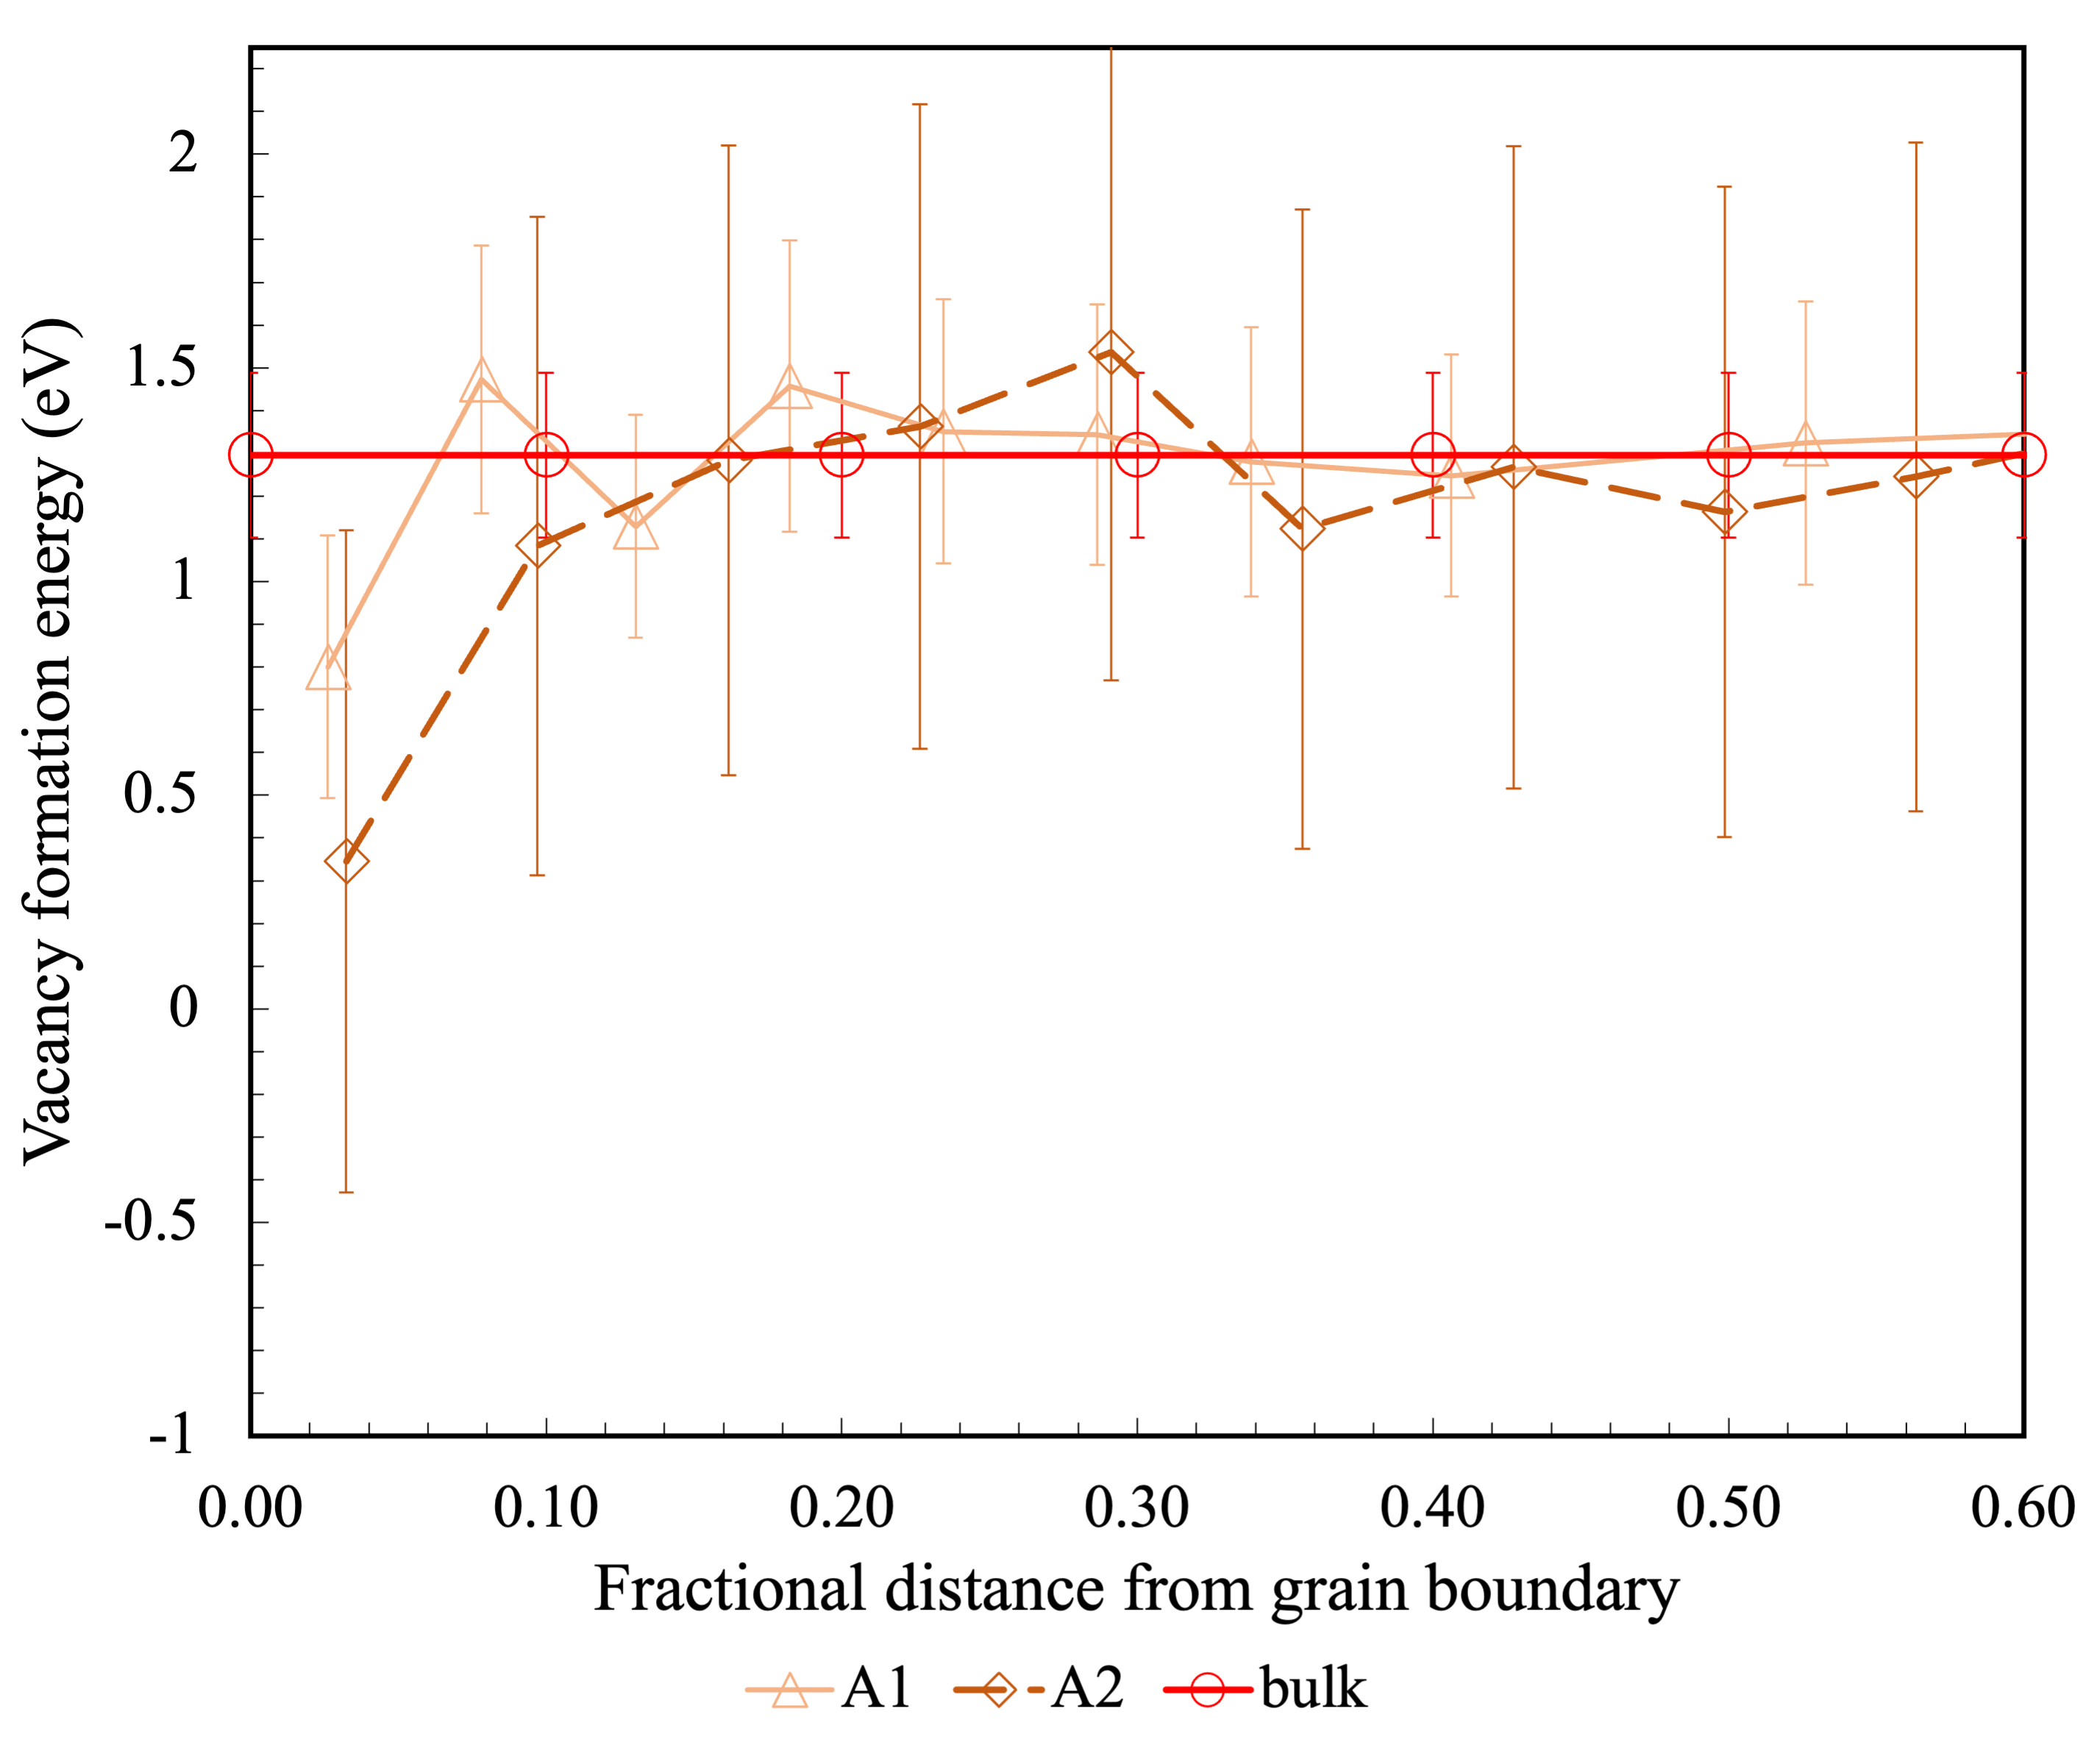
\includegraphics[width = 2.0in]{A_500_Vacan.png}} 
%DIFDELCMD < \subfloat[]{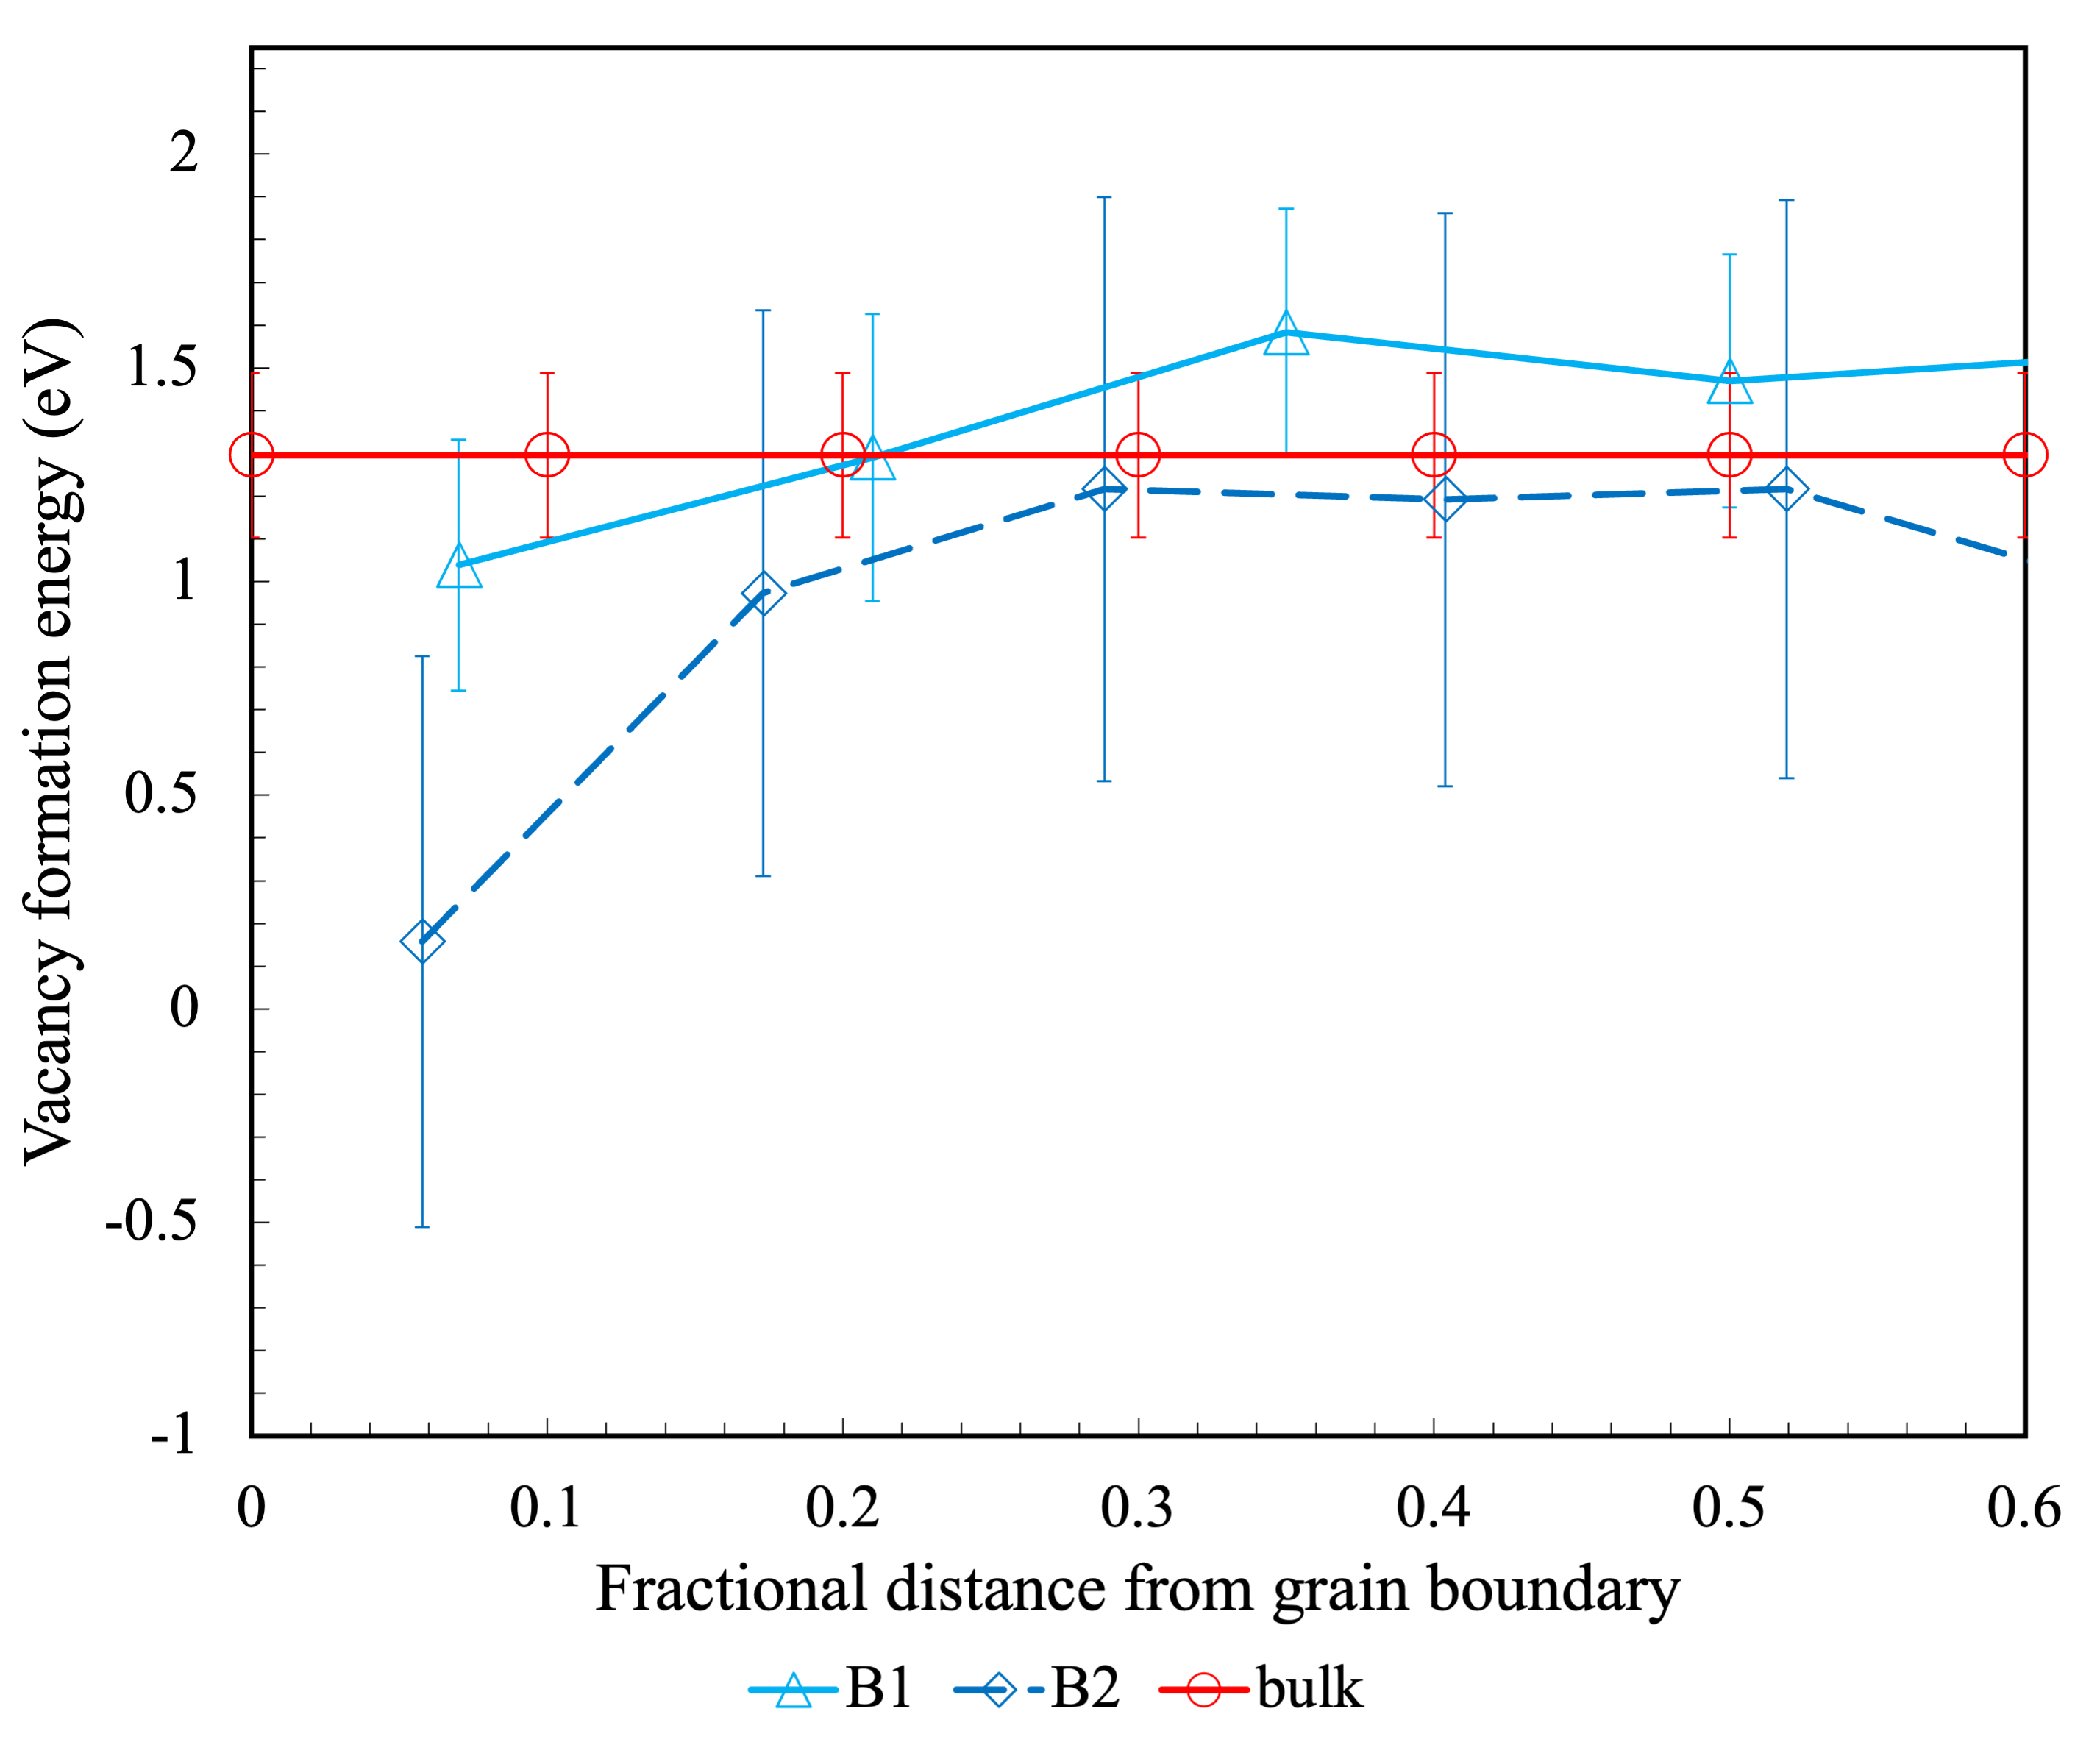
\includegraphics[width = 2.0in]{B_500_Vacan.png}}
%DIFDELCMD < \subfloat[]{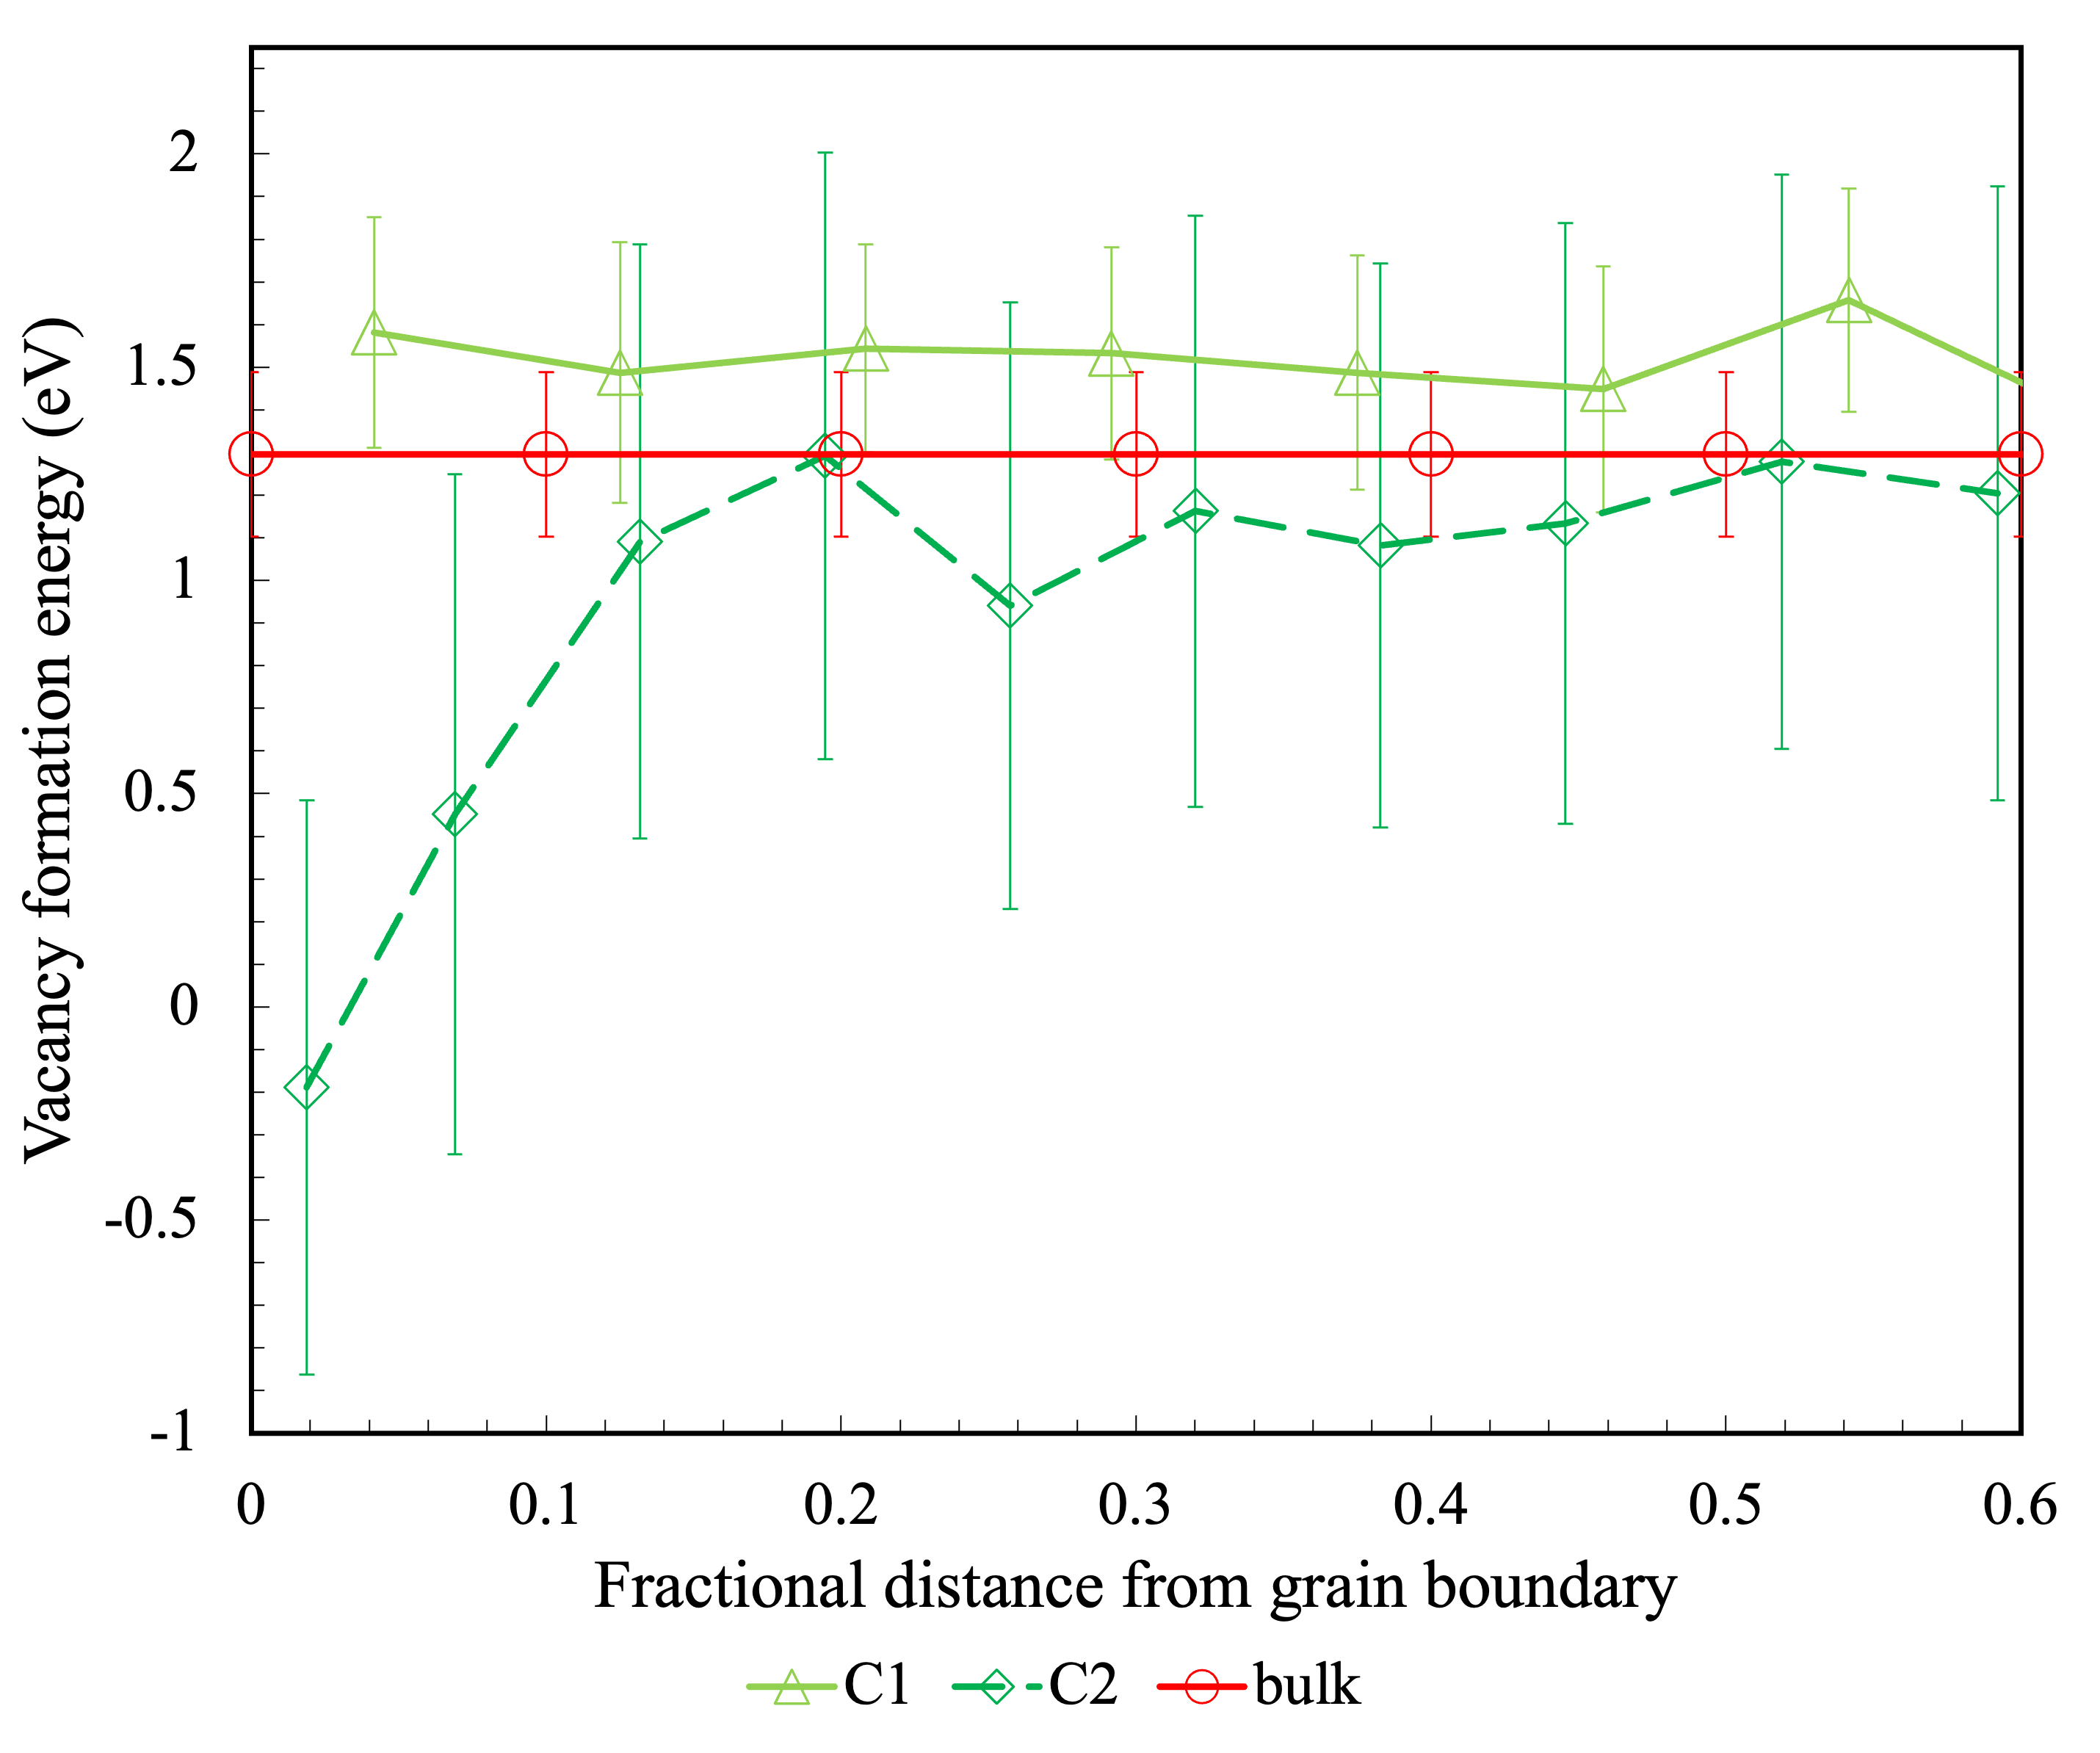
\includegraphics[width = 2.0in]{C_500_Vacan.png}}
%DIFDELCMD < %%%
\DIFdelendFL \DIFaddbeginFL \subfloat[]{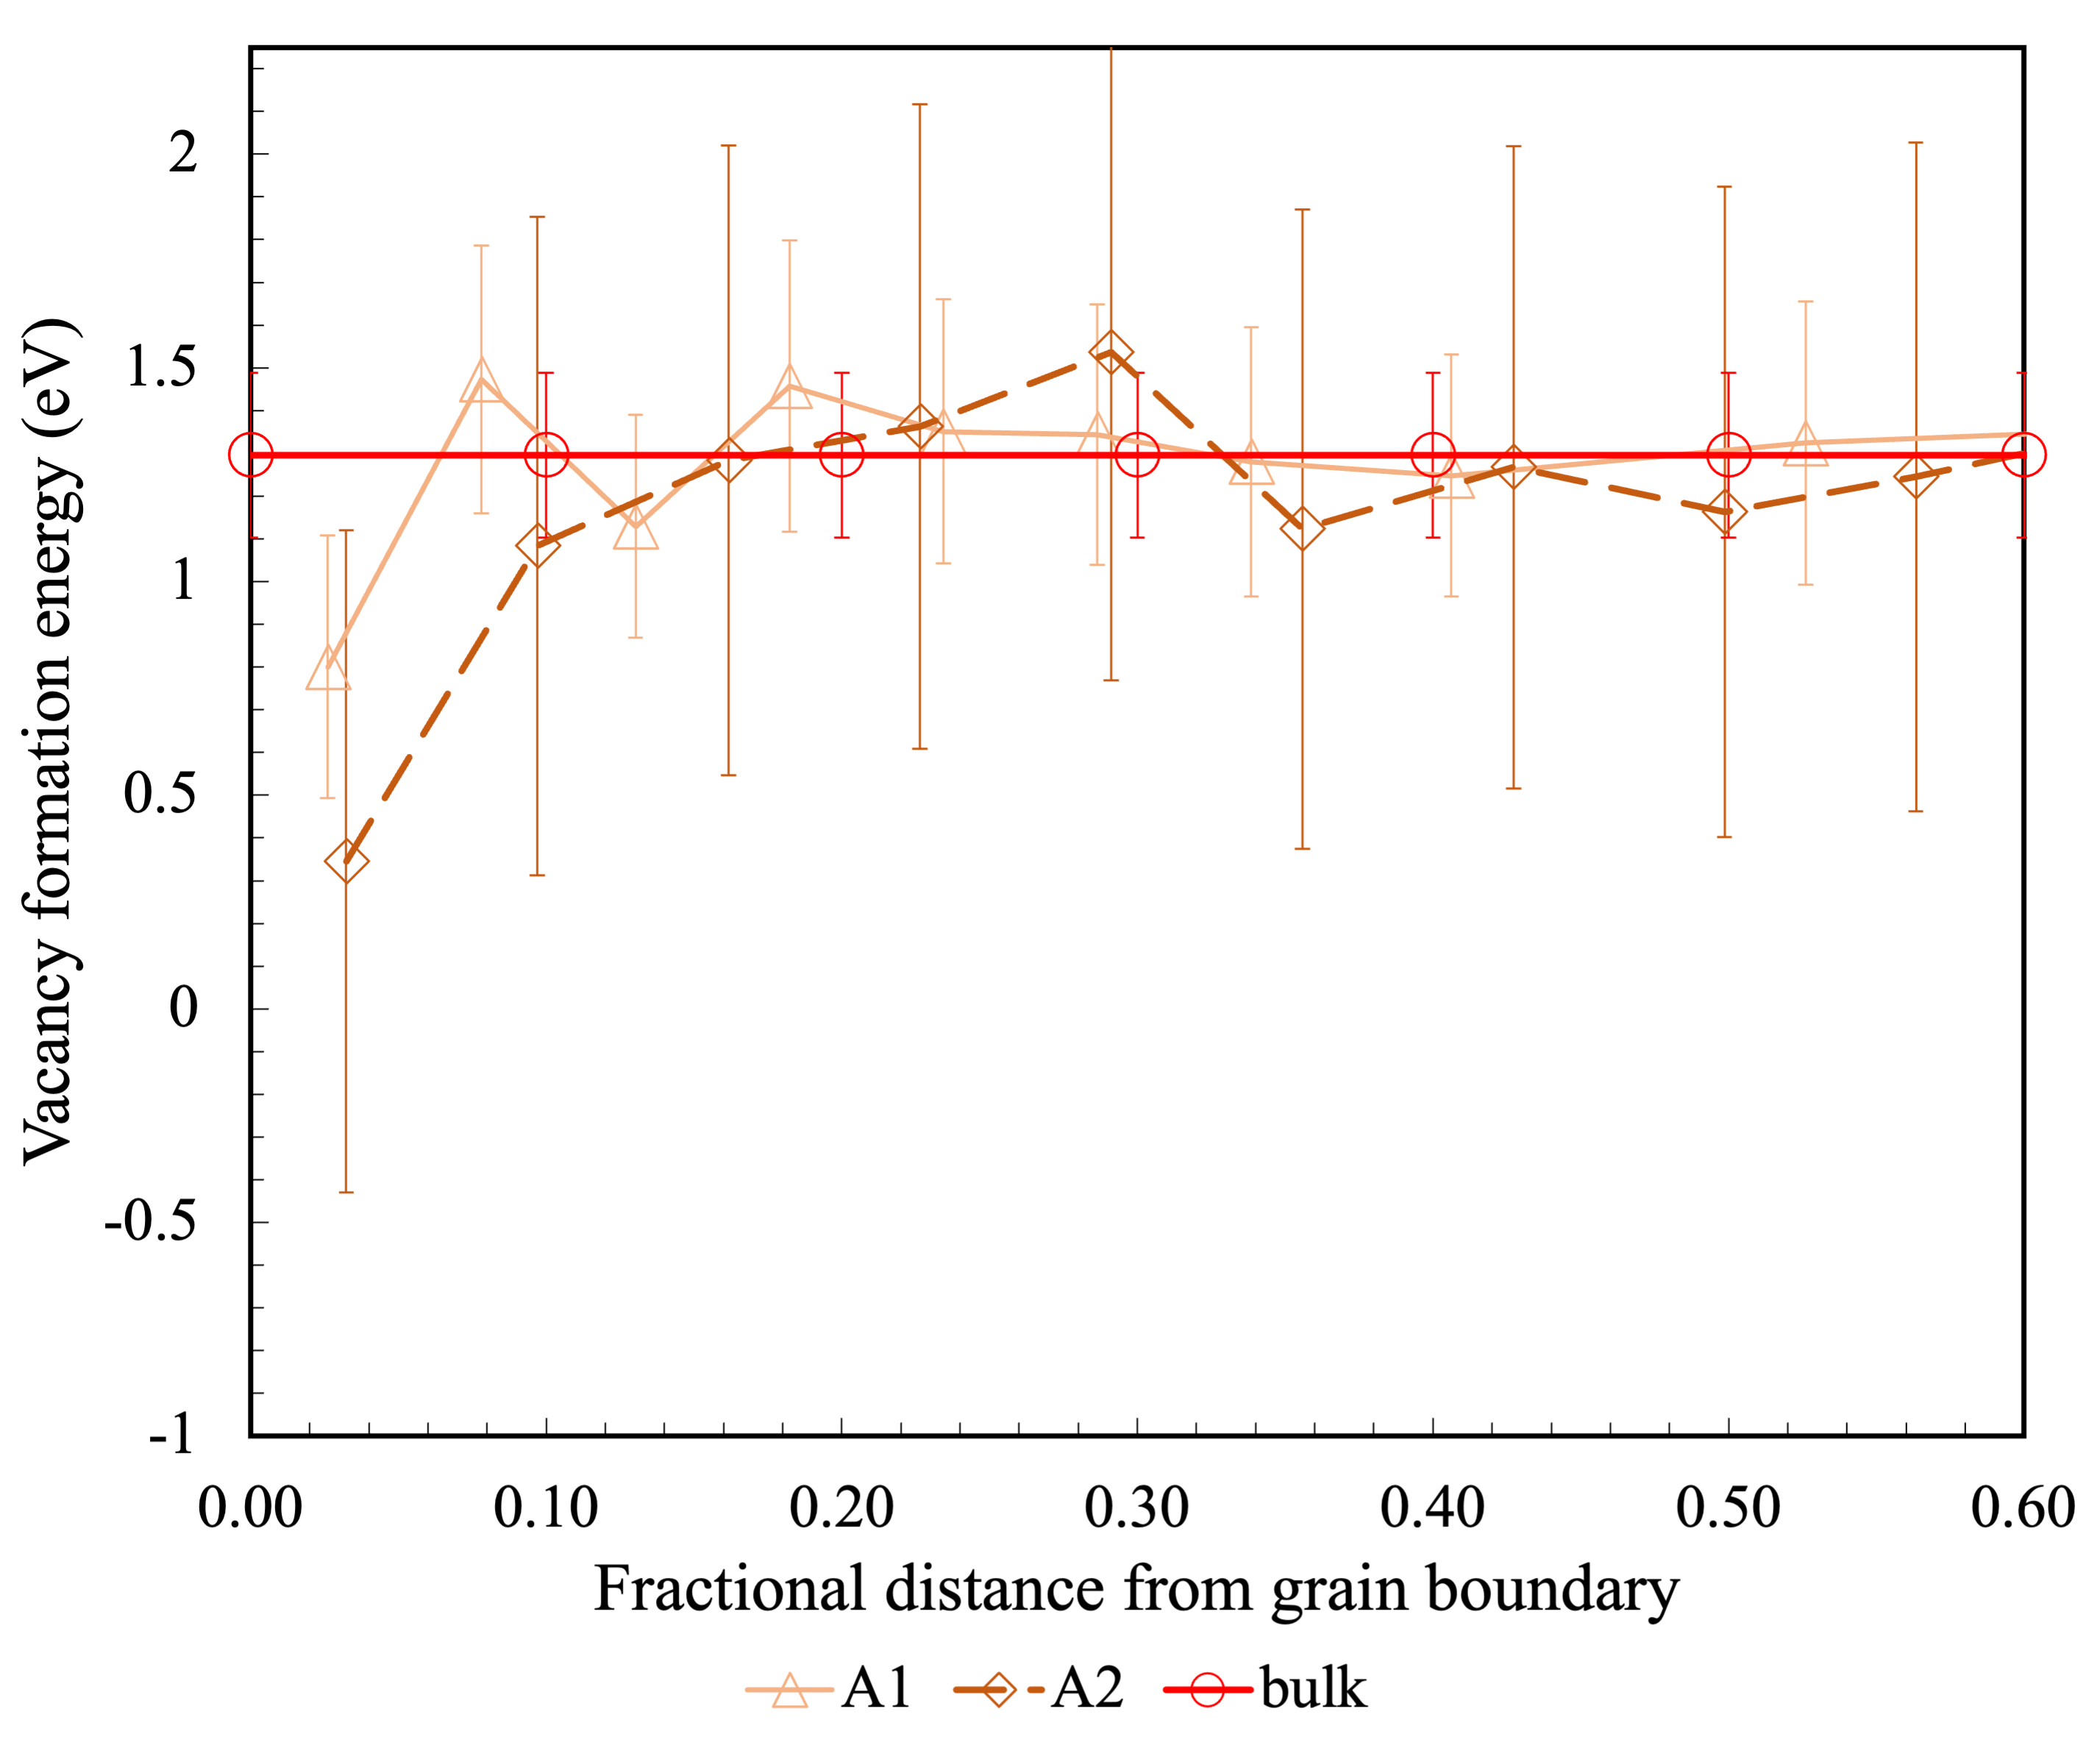
\includegraphics[width = 2.0in]{3_A_500_Vacan.png}} 
\subfloat[]{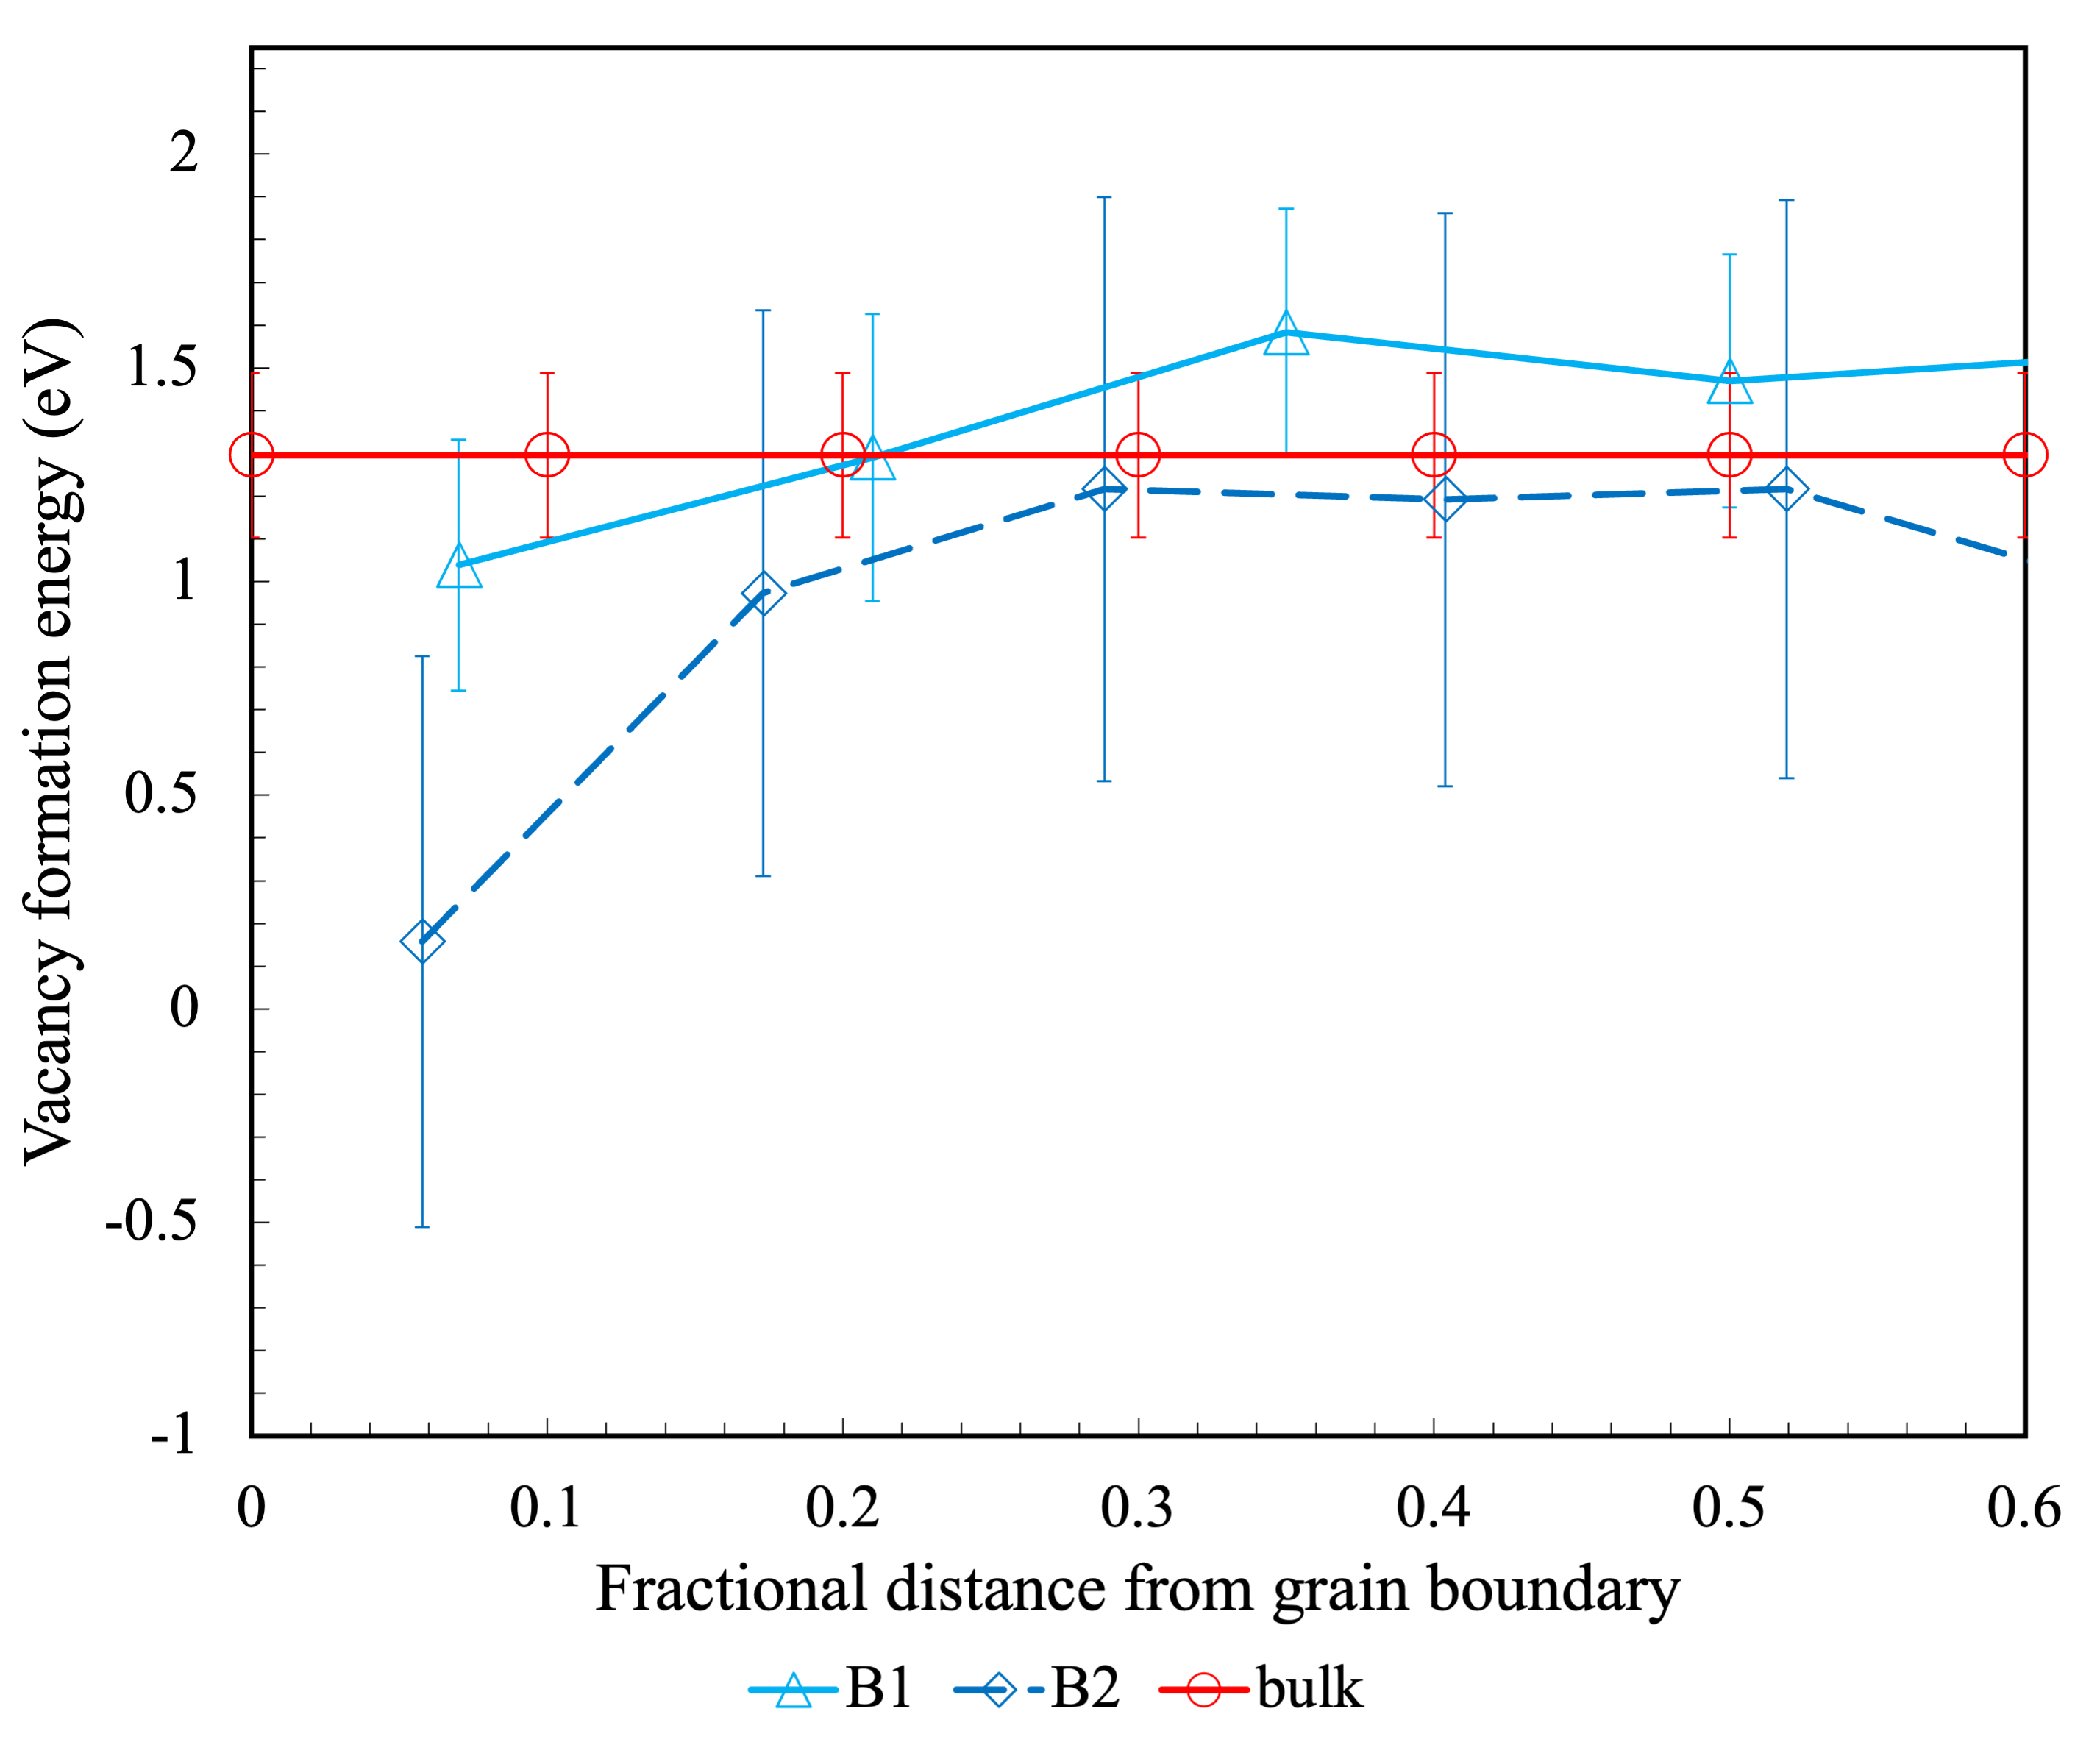
\includegraphics[width = 2.0in]{3_B_500_Vacan.png}}
\subfloat[]{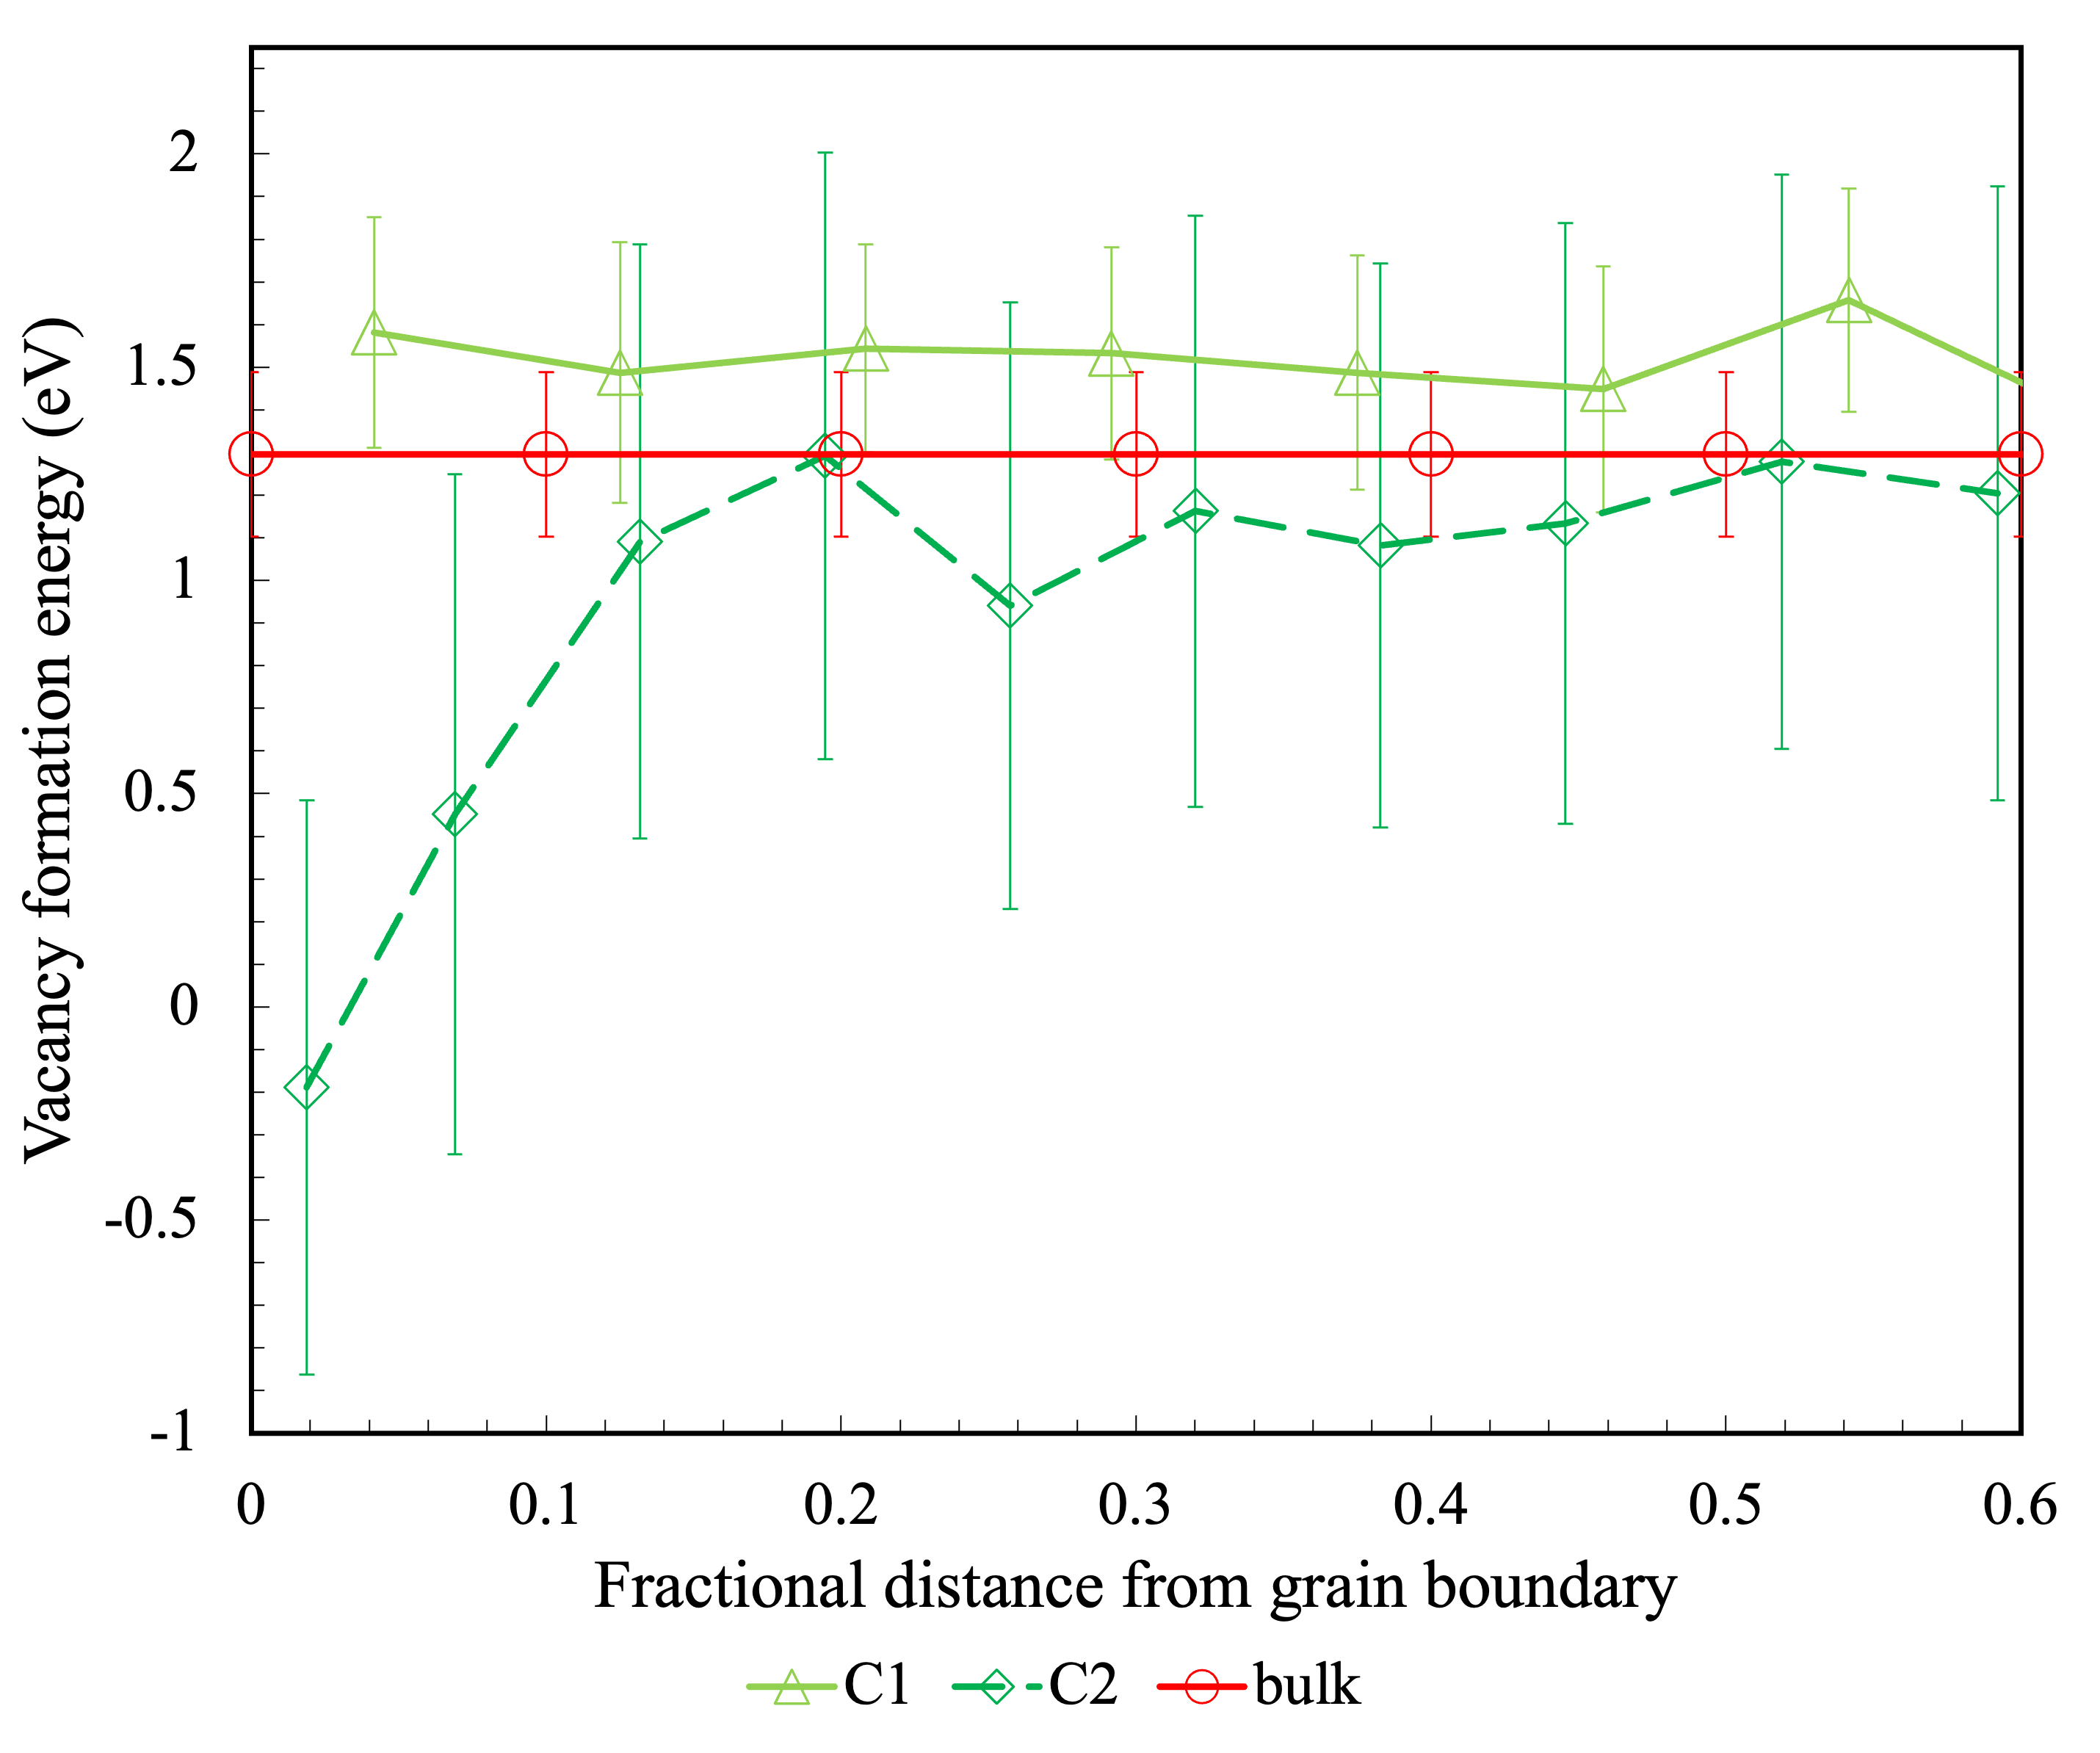
\includegraphics[width = 2.0in]{3_C_500_Vacan.png}}
\DIFaddendFL \caption{Average formation energy of a vacancy at 500 K as a function of fractional distance from (a) type A, (b) type B, and (c) type C GB core. The red line shows the formation energy of a vacancy in pristine $\alpha$-U. The error bars show twice the standard error.}
\label{fig:Seg_vacancy_500}
\end{figure}

\par Error bars in \Cref{fig:Seg_inter_500,fig:Seg_vacancy_500} are twice the standard error of the mean. This is a propagated standard error considering both the error from the total energy of the pristine GB and a GB with a point defect. A system with GBs is not an equilibrium system but rather a metastable system, which is a possible reason for the large error bars of the $E_{\mathrm{f}}$. As the temperature increases, the magnitude of the error bars further increases due to increased thermal fluctuations.

\subsubsection{Segregation Energies}
\par In order to describe how a GB will act as a sink, both the magnitude of the $E_{\mathrm{s}}$ calculated via \Cref{eq:eform2} and the distance from the GB core where there is a non-zero $E_{\mathrm{s}}$ are important. Since $E_{\mathrm{f}}$ reaches a minimum value near the GB core, the highest $E_{\mathrm{s}}$ is observed at the GB core. The highest $E_{\mathrm{s}}$ of vacancies and interstitials at different temperatures for the studied GBs are shown in \Cref{fig:Seg}. The dashed line in the figure denotes high-energy GBs, the solid line low-energy GBs, the closed symbol is for an interstitial, and the open symbol is for a vacancy. In the following, the highest $E_{\mathrm{s}}$ (the value at the core) is referred to simply as the $E_{\mathrm{s}}$.

\begin{figure}[h!]
\centering
\DIFdelbeginFL %DIFDELCMD < \subfloat[]{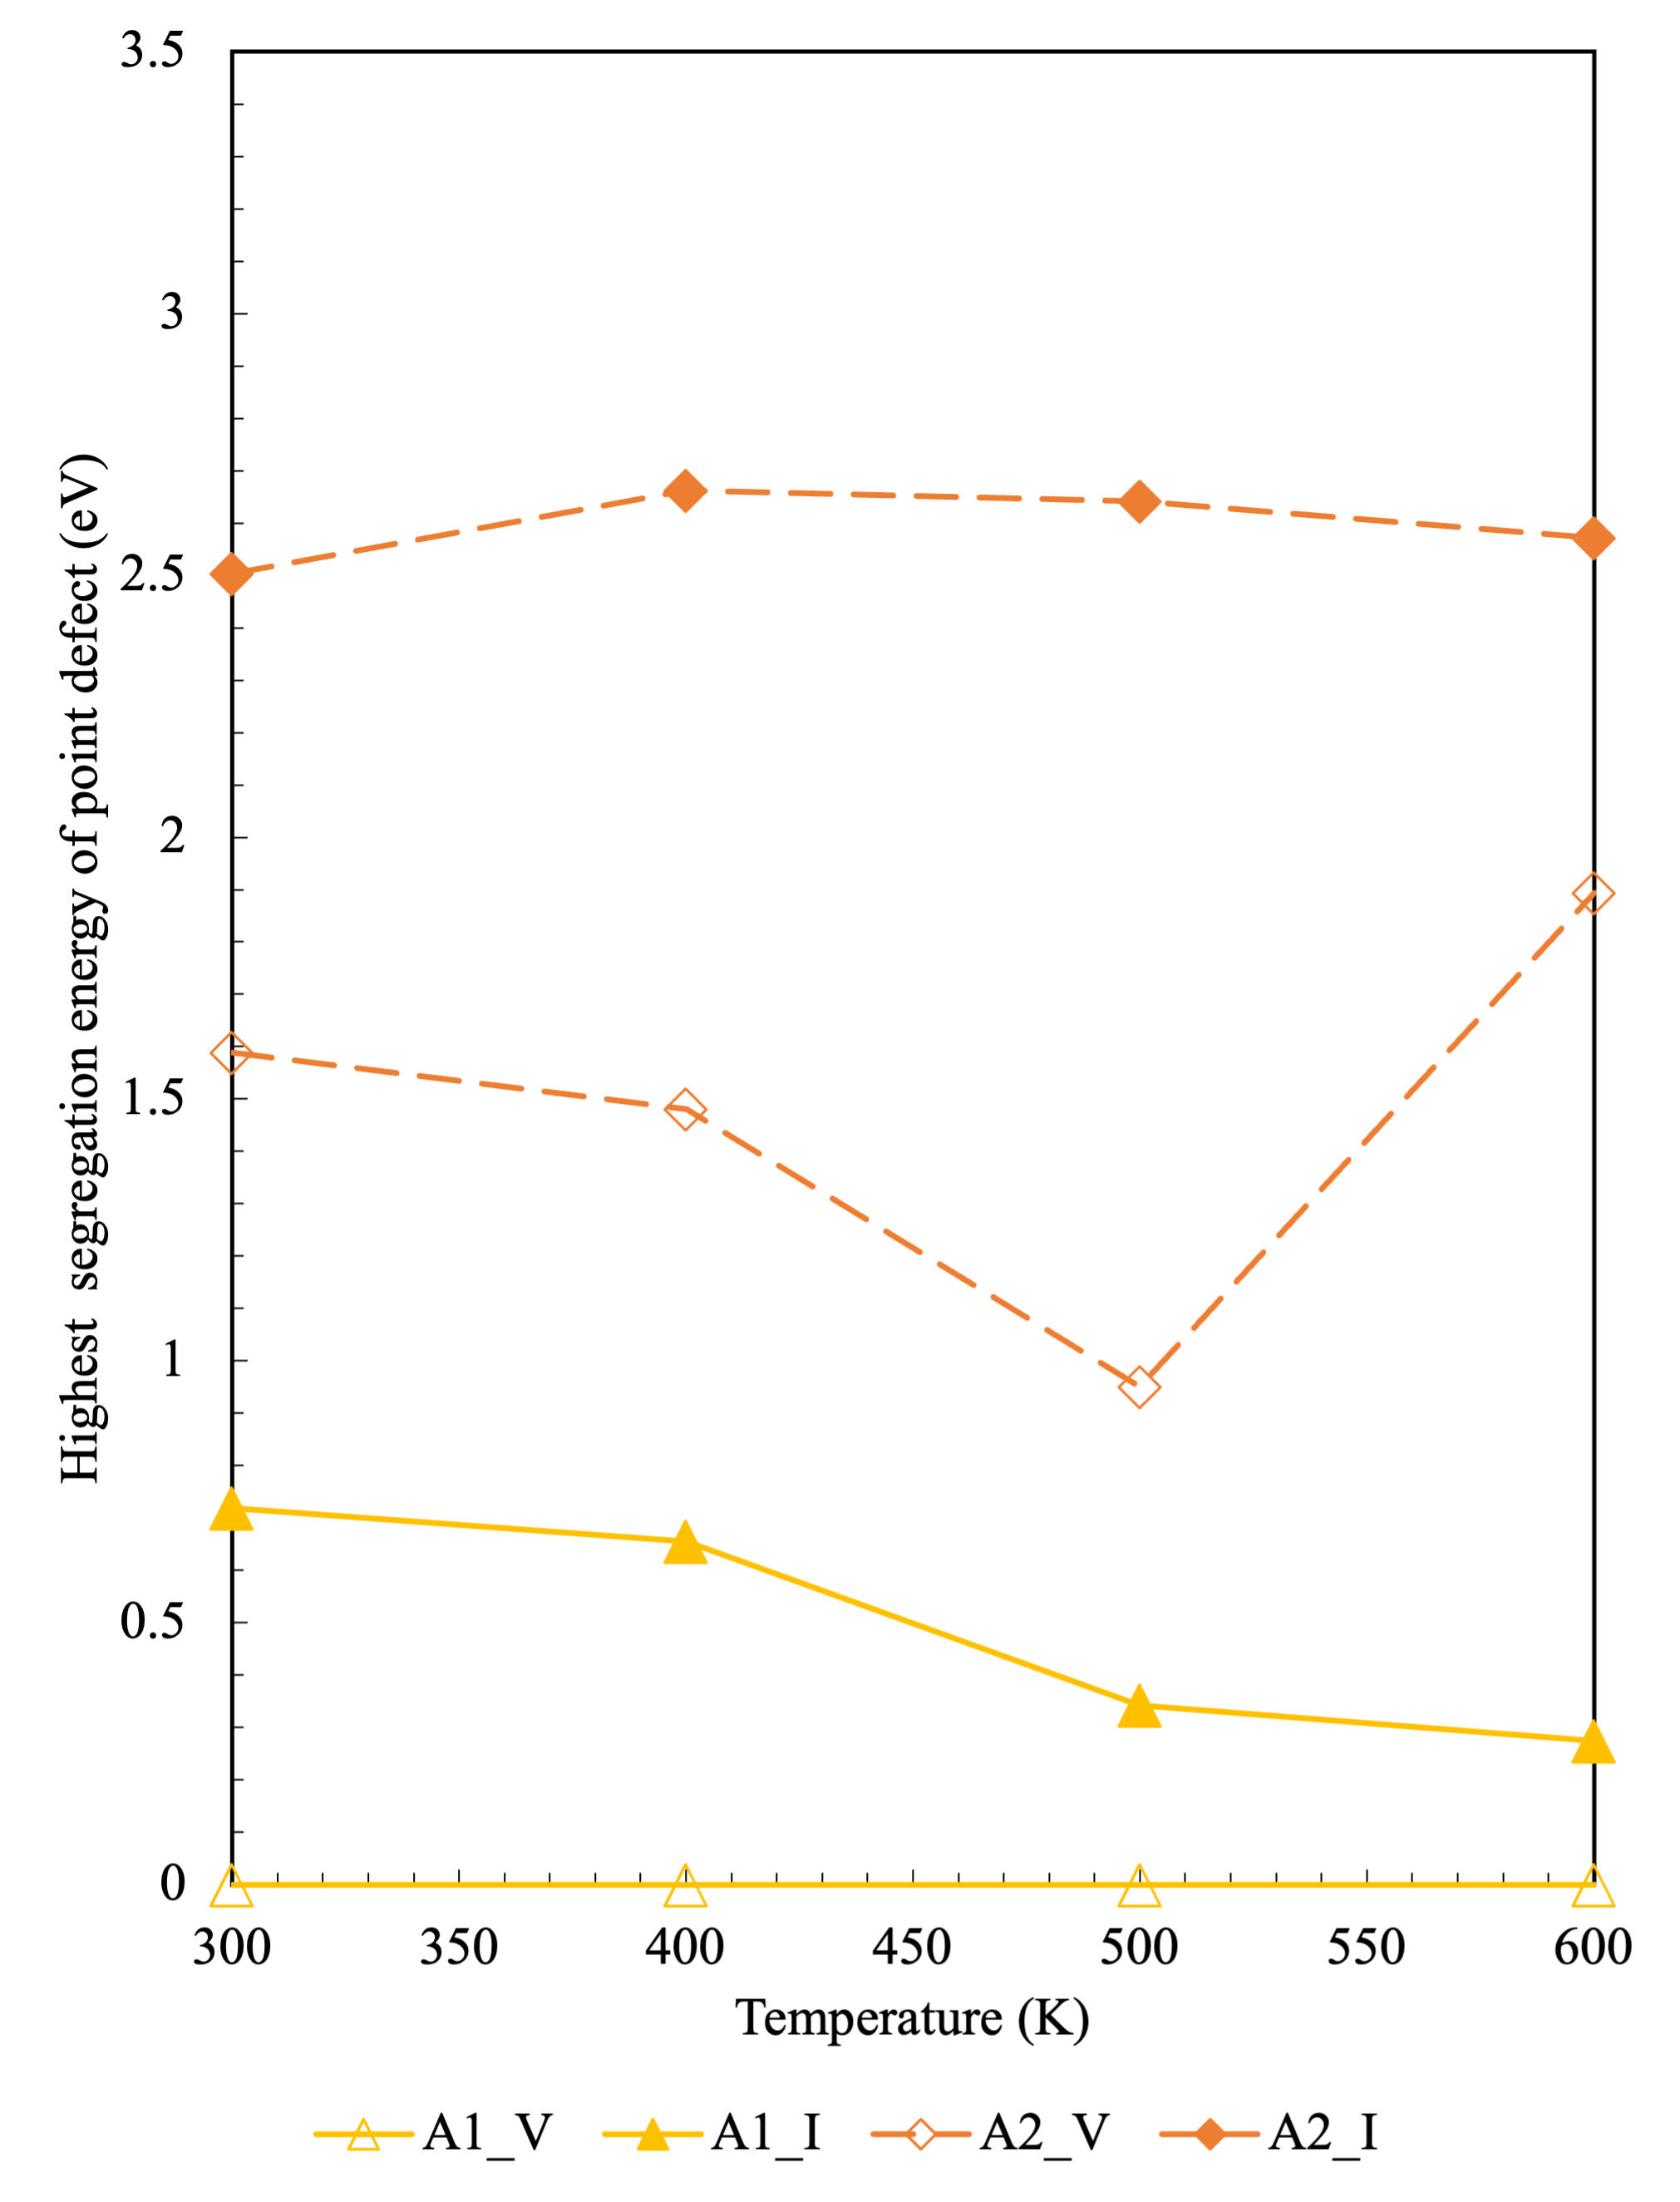
\includegraphics[width = 2.25in]{A_SE.png}}
%DIFDELCMD < \subfloat[]{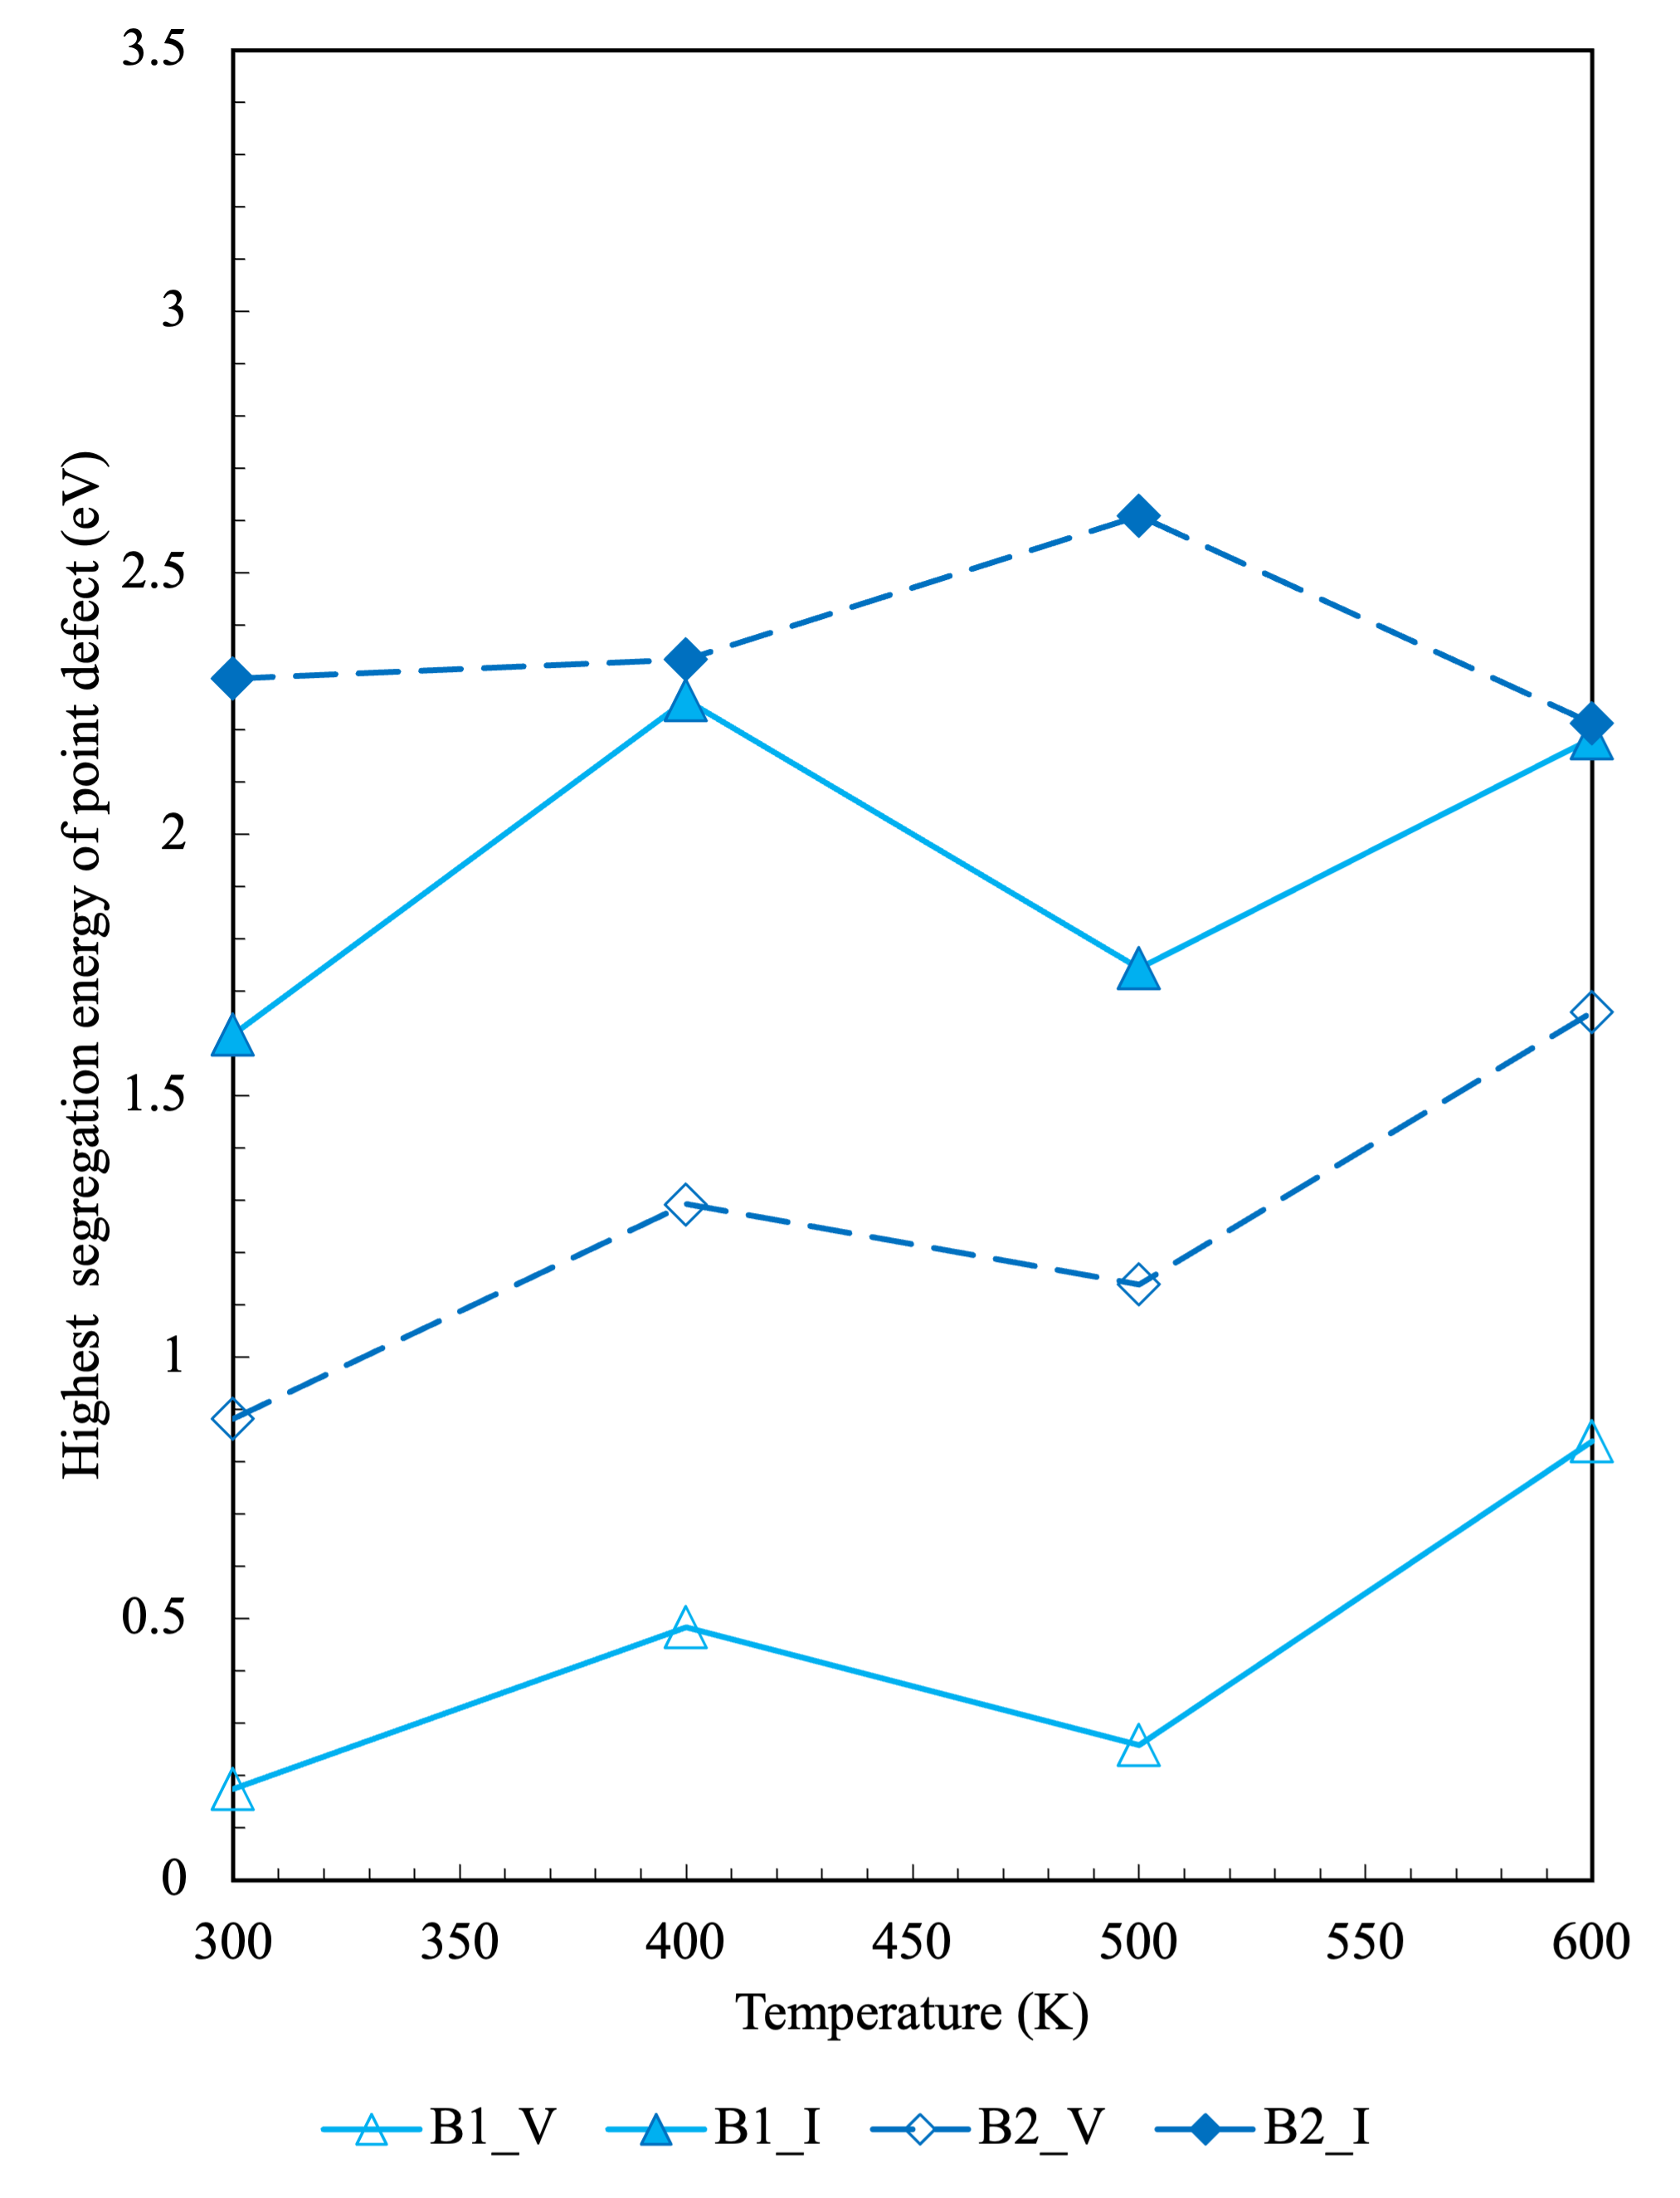
\includegraphics[width = 2.25in]{B_SE.png}} 
%DIFDELCMD < \subfloat[]{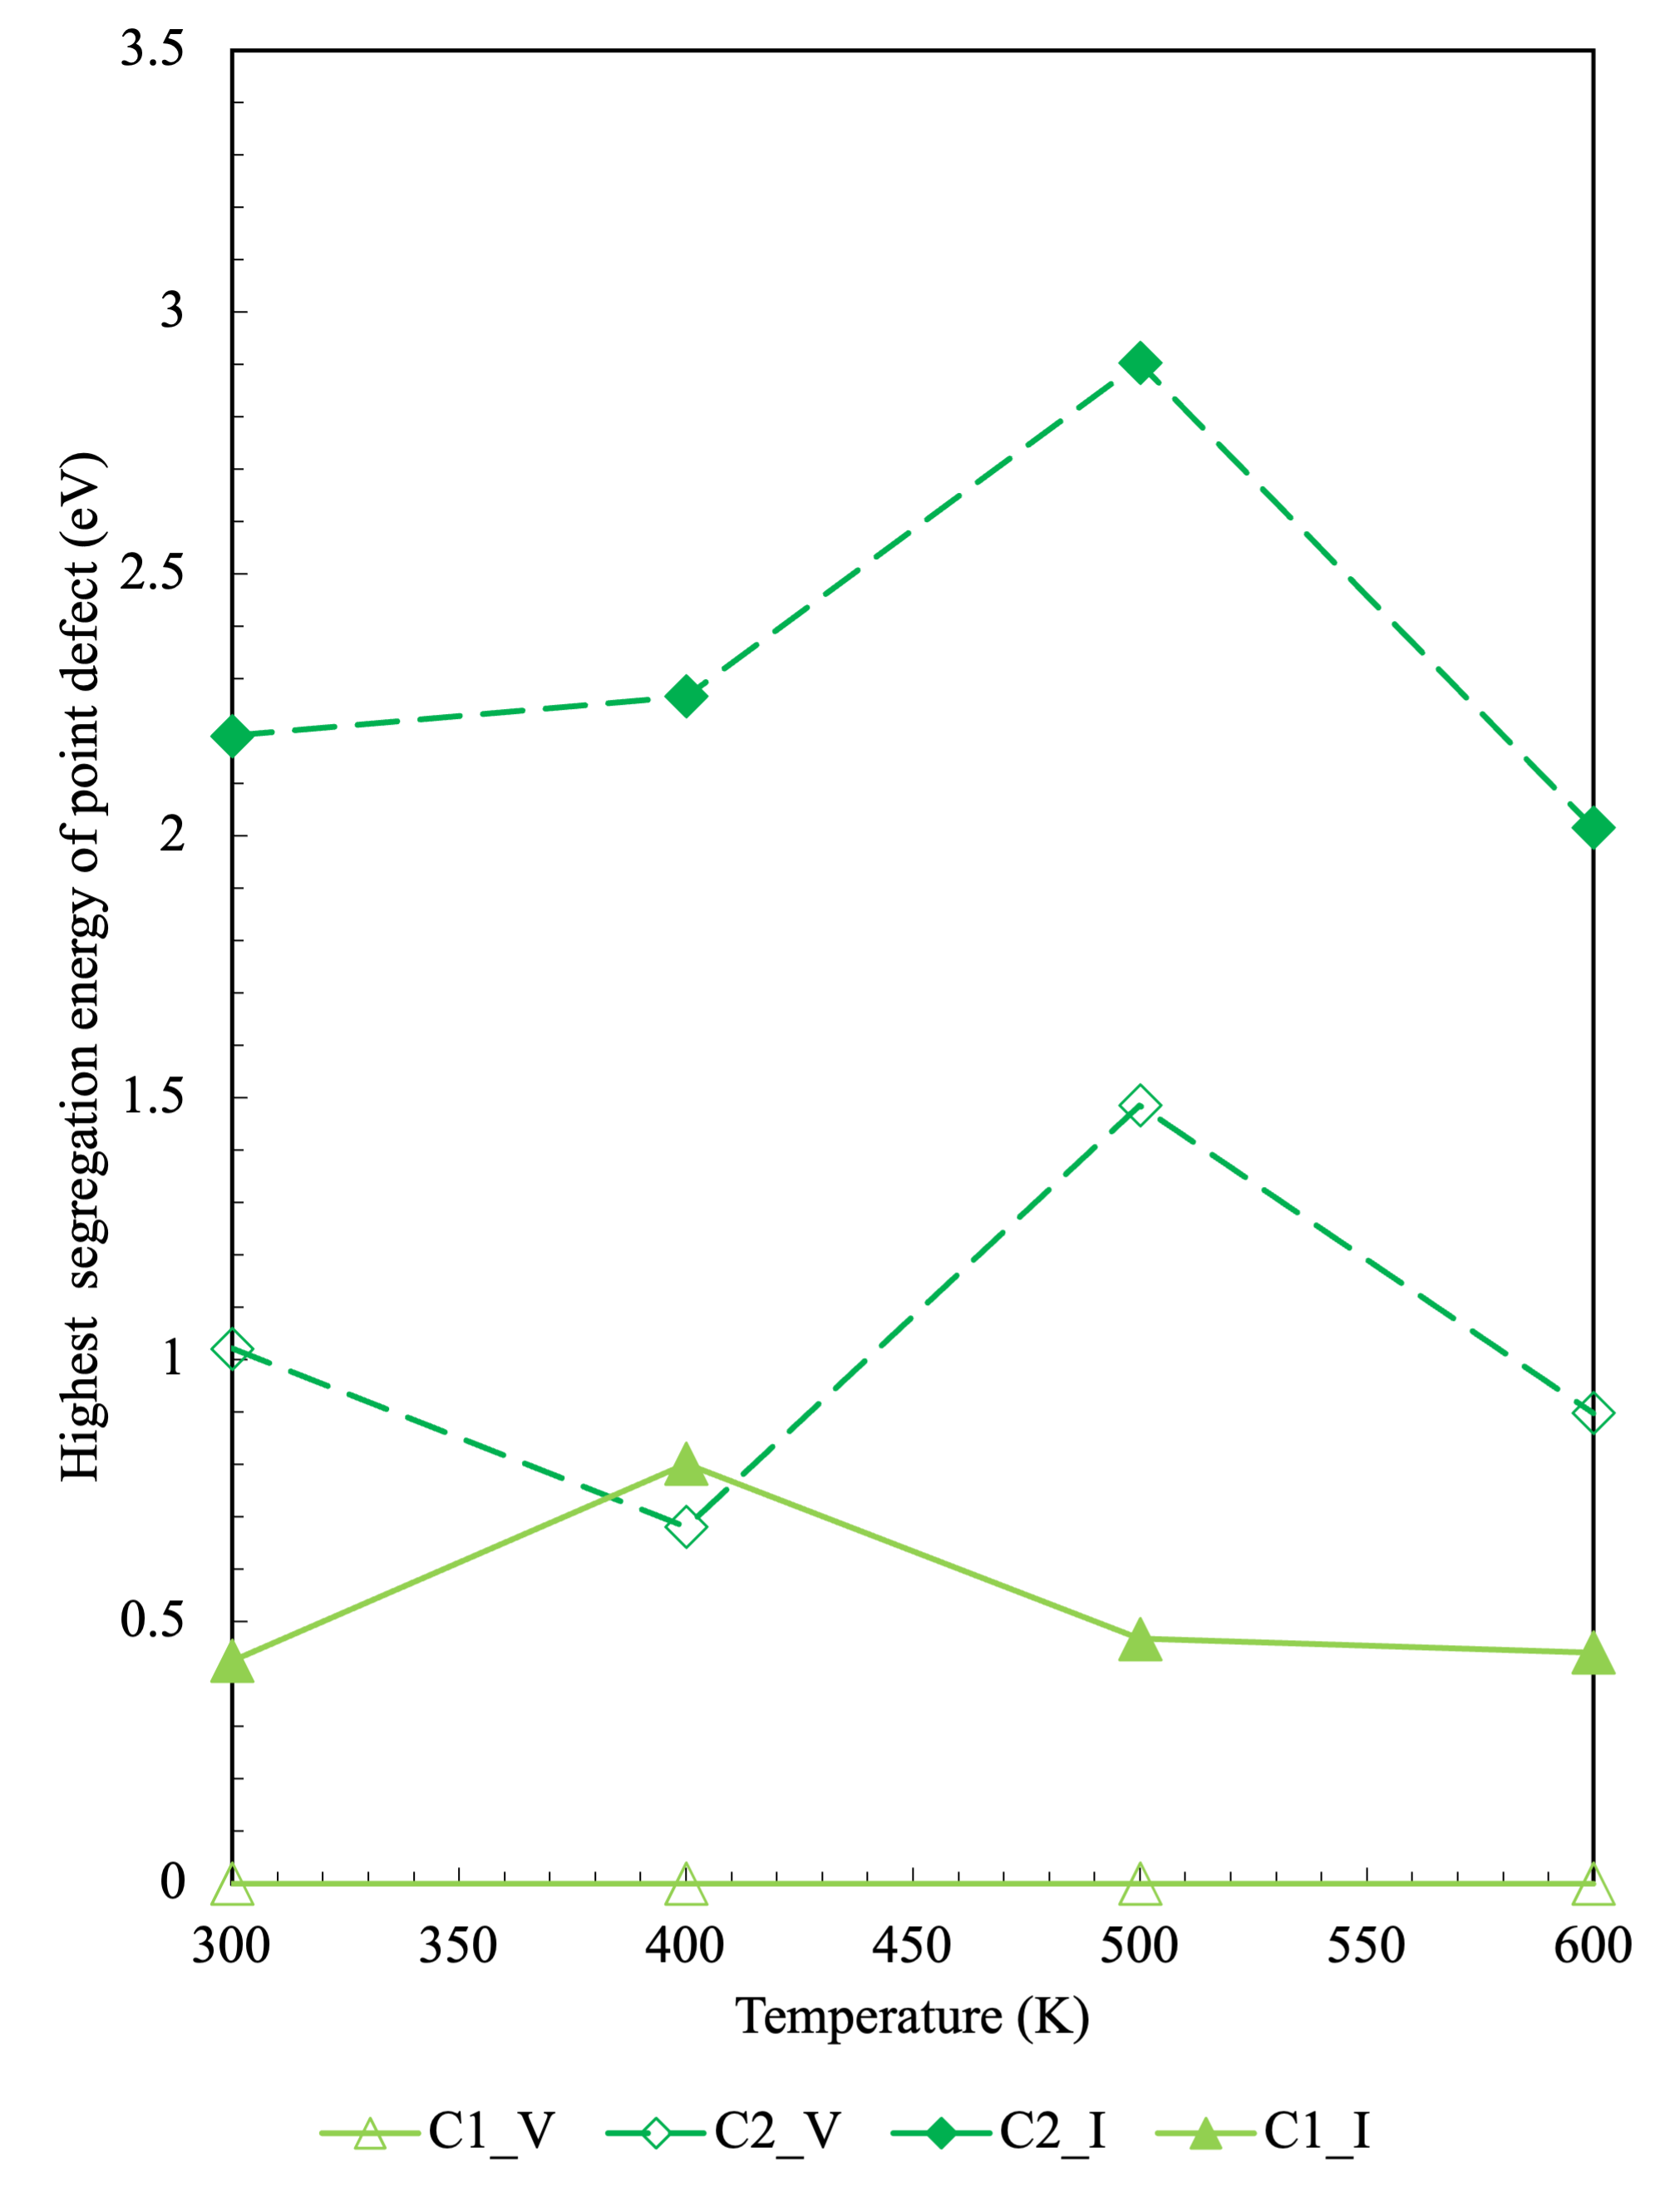
\includegraphics[width = 2.25in]{C_SE.png}}%%%
\DIFdelendFL \DIFaddbeginFL \subfloat[]{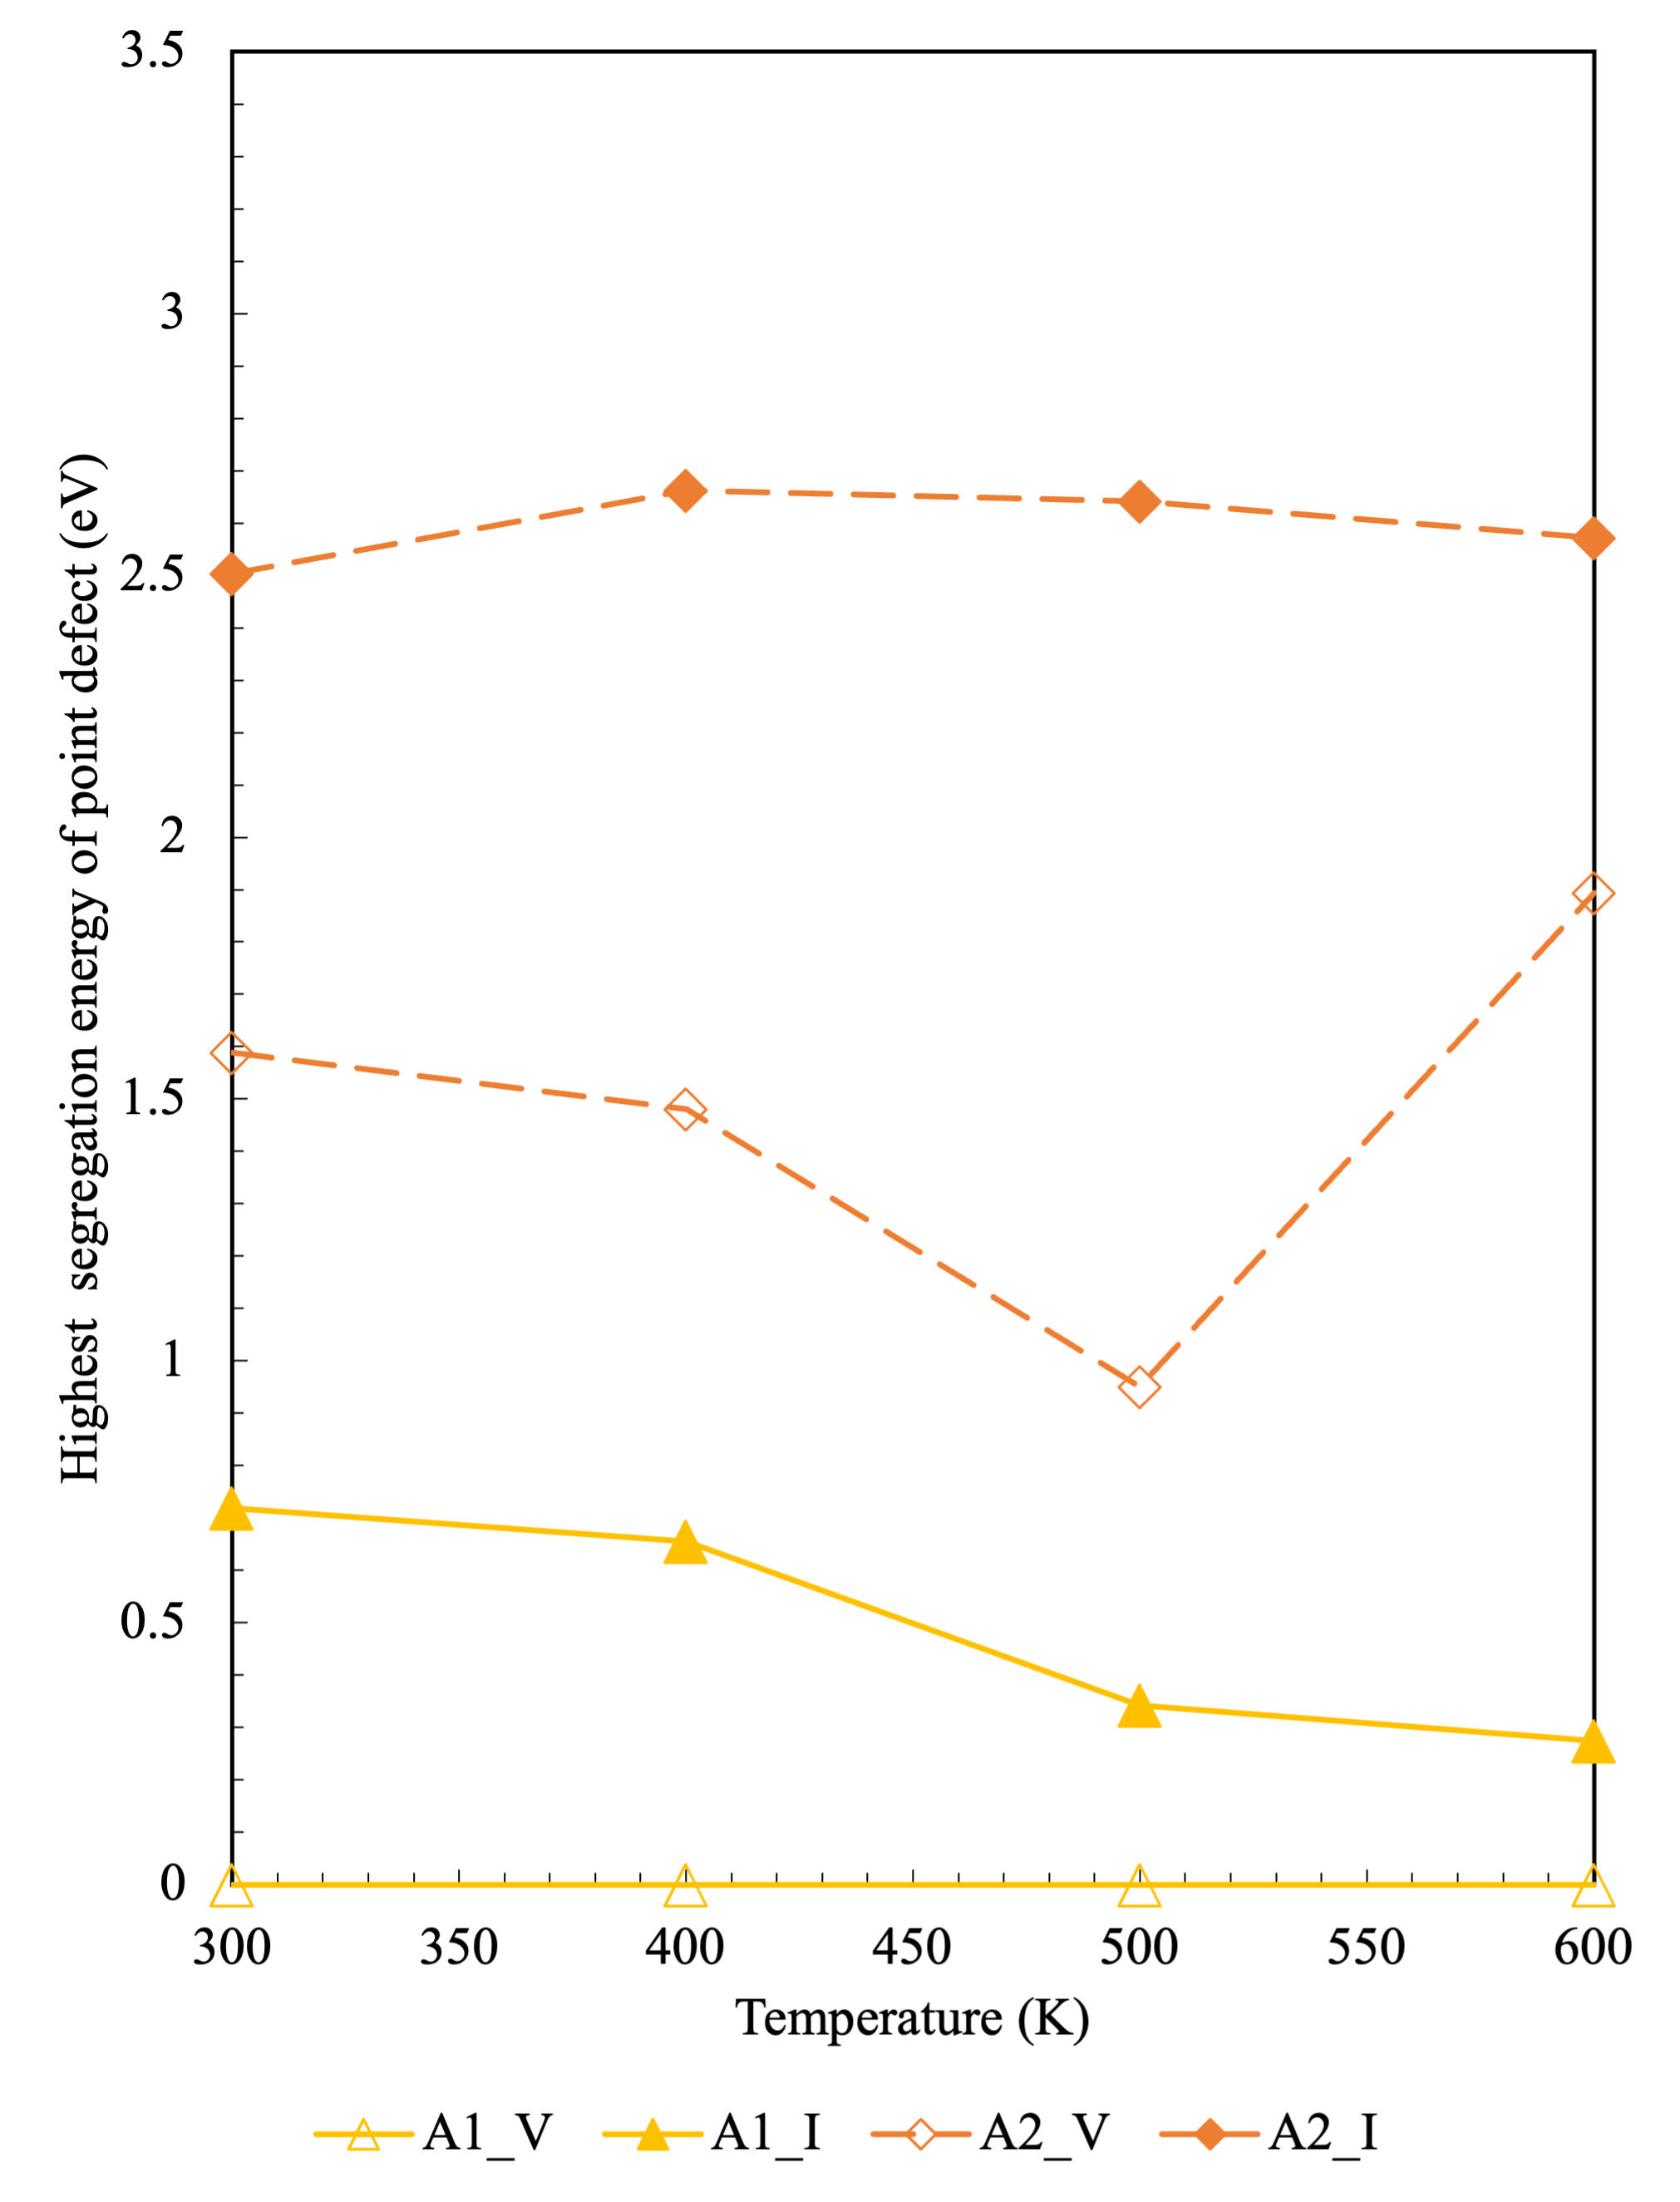
\includegraphics[width = 2.25in]{4_A_SE.png}}
\subfloat[]{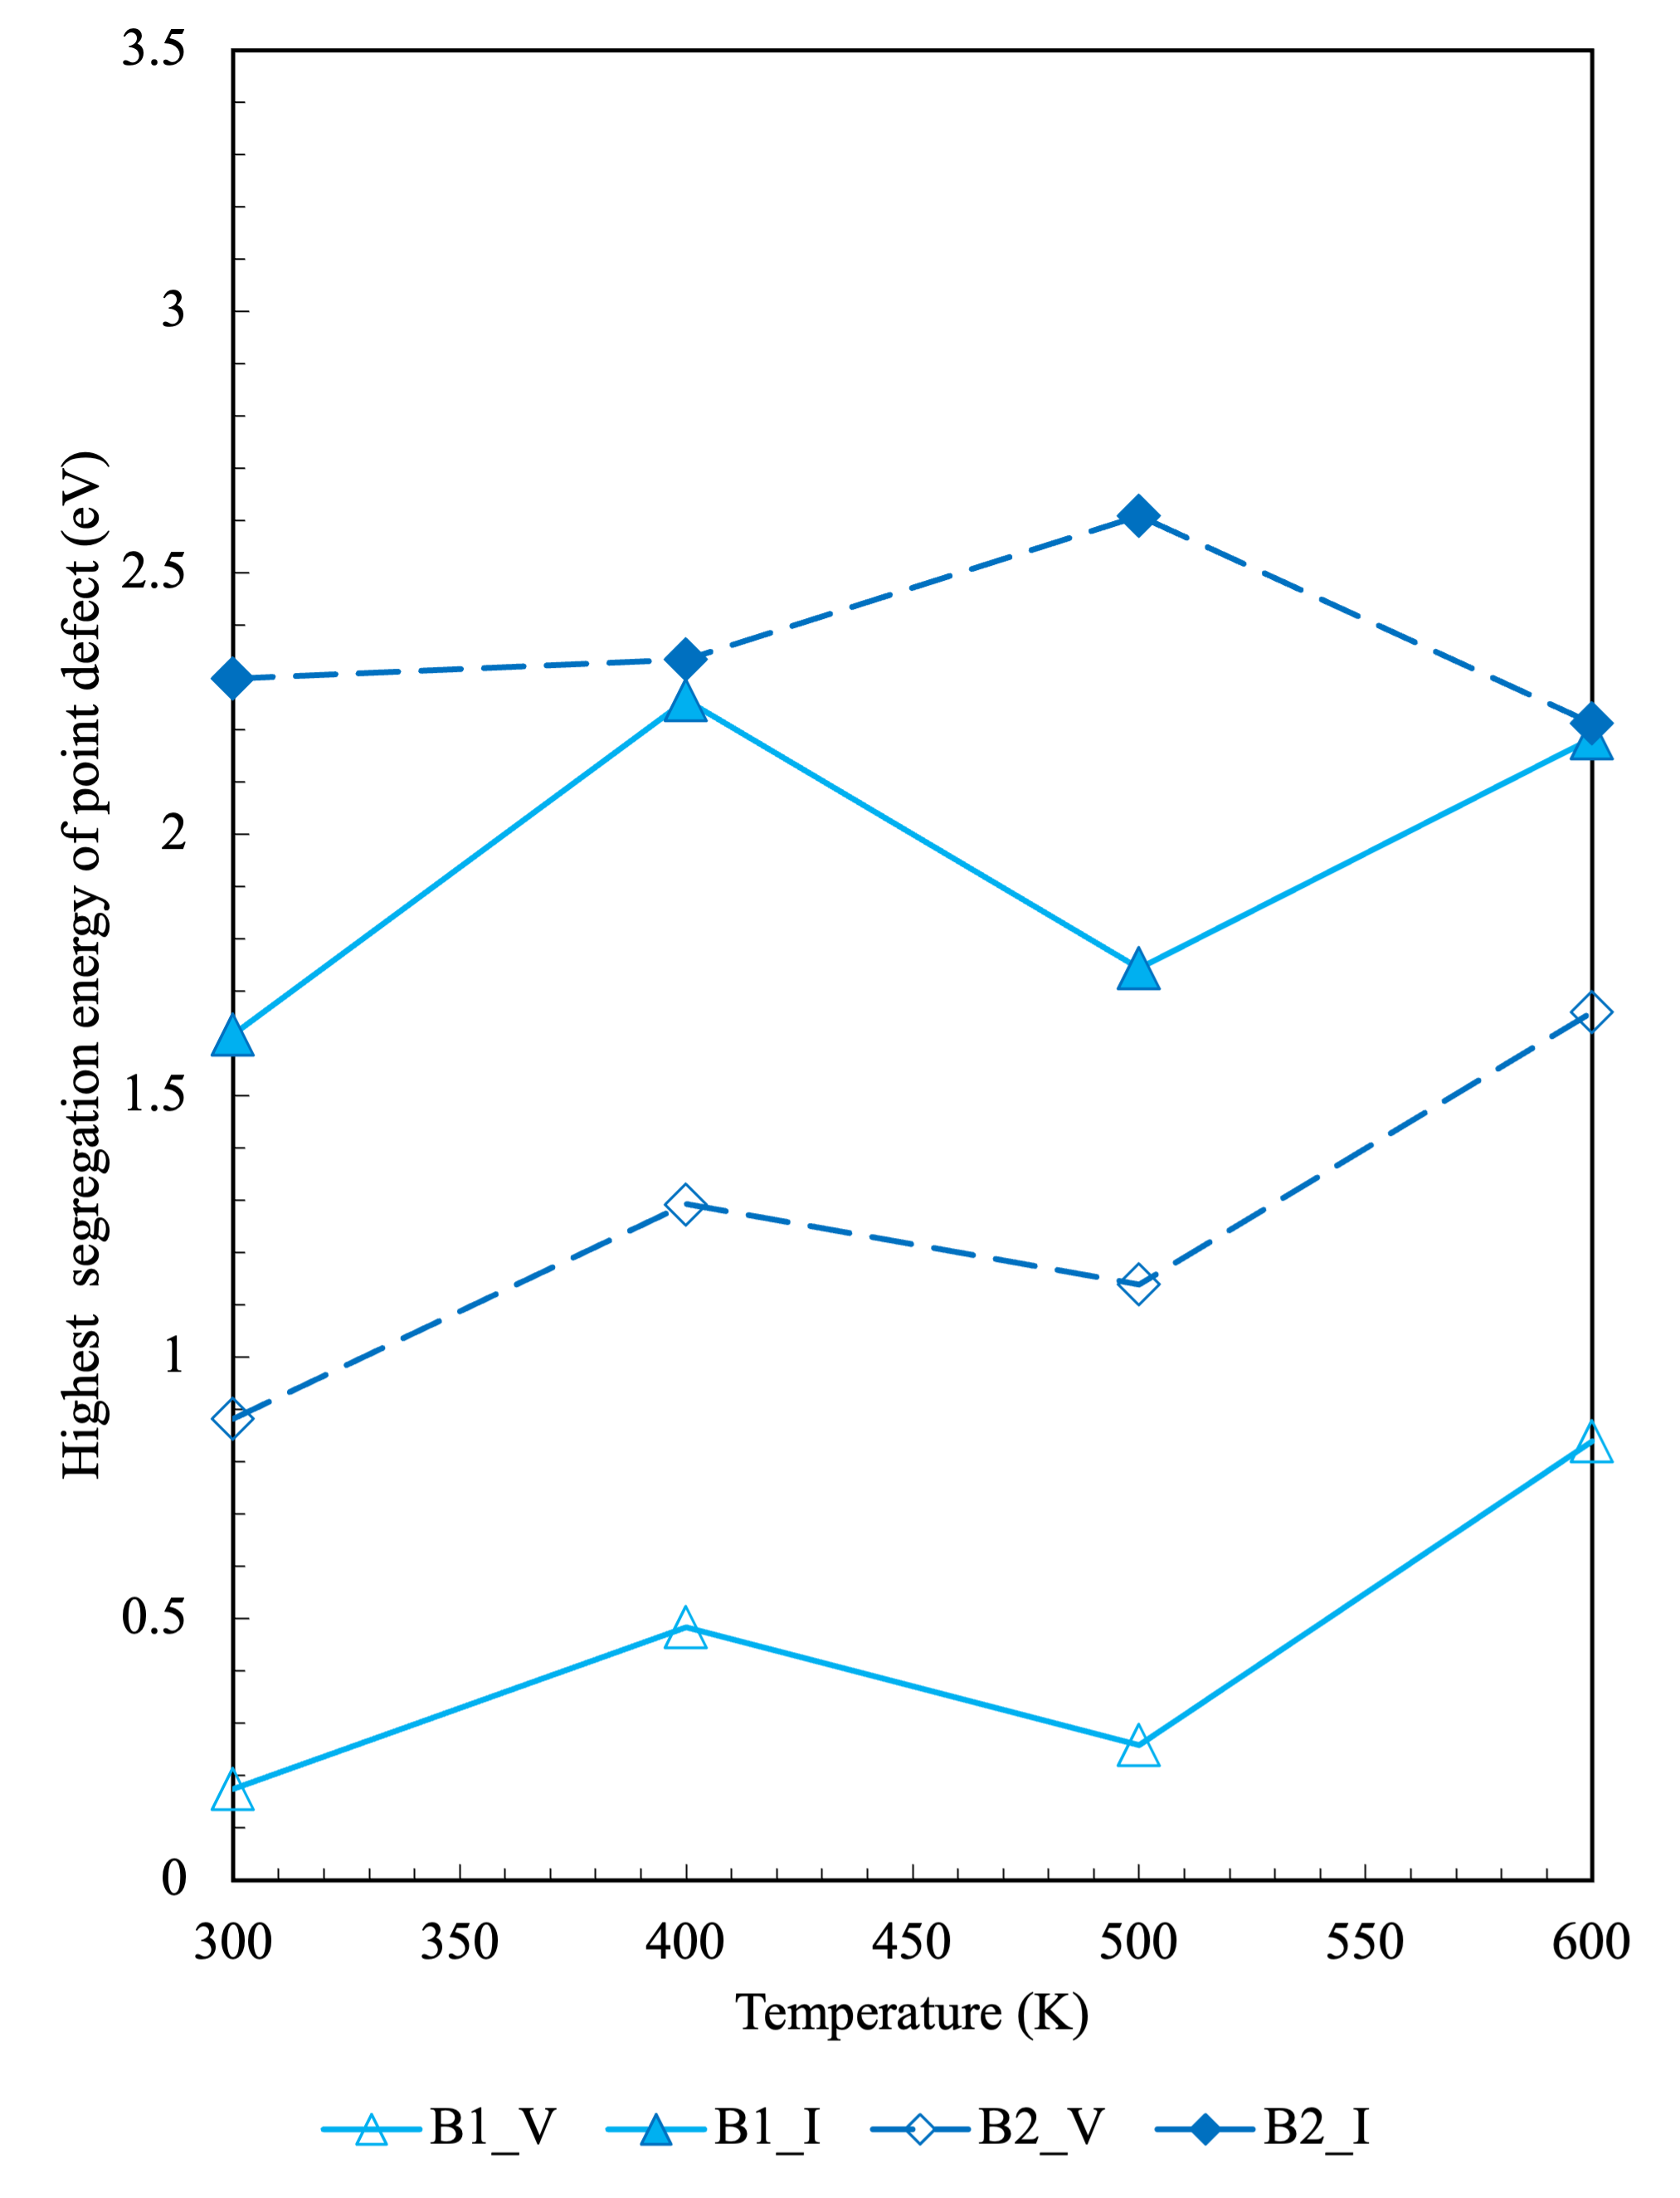
\includegraphics[width = 2.25in]{4_B_SE.png}} 
\subfloat[]{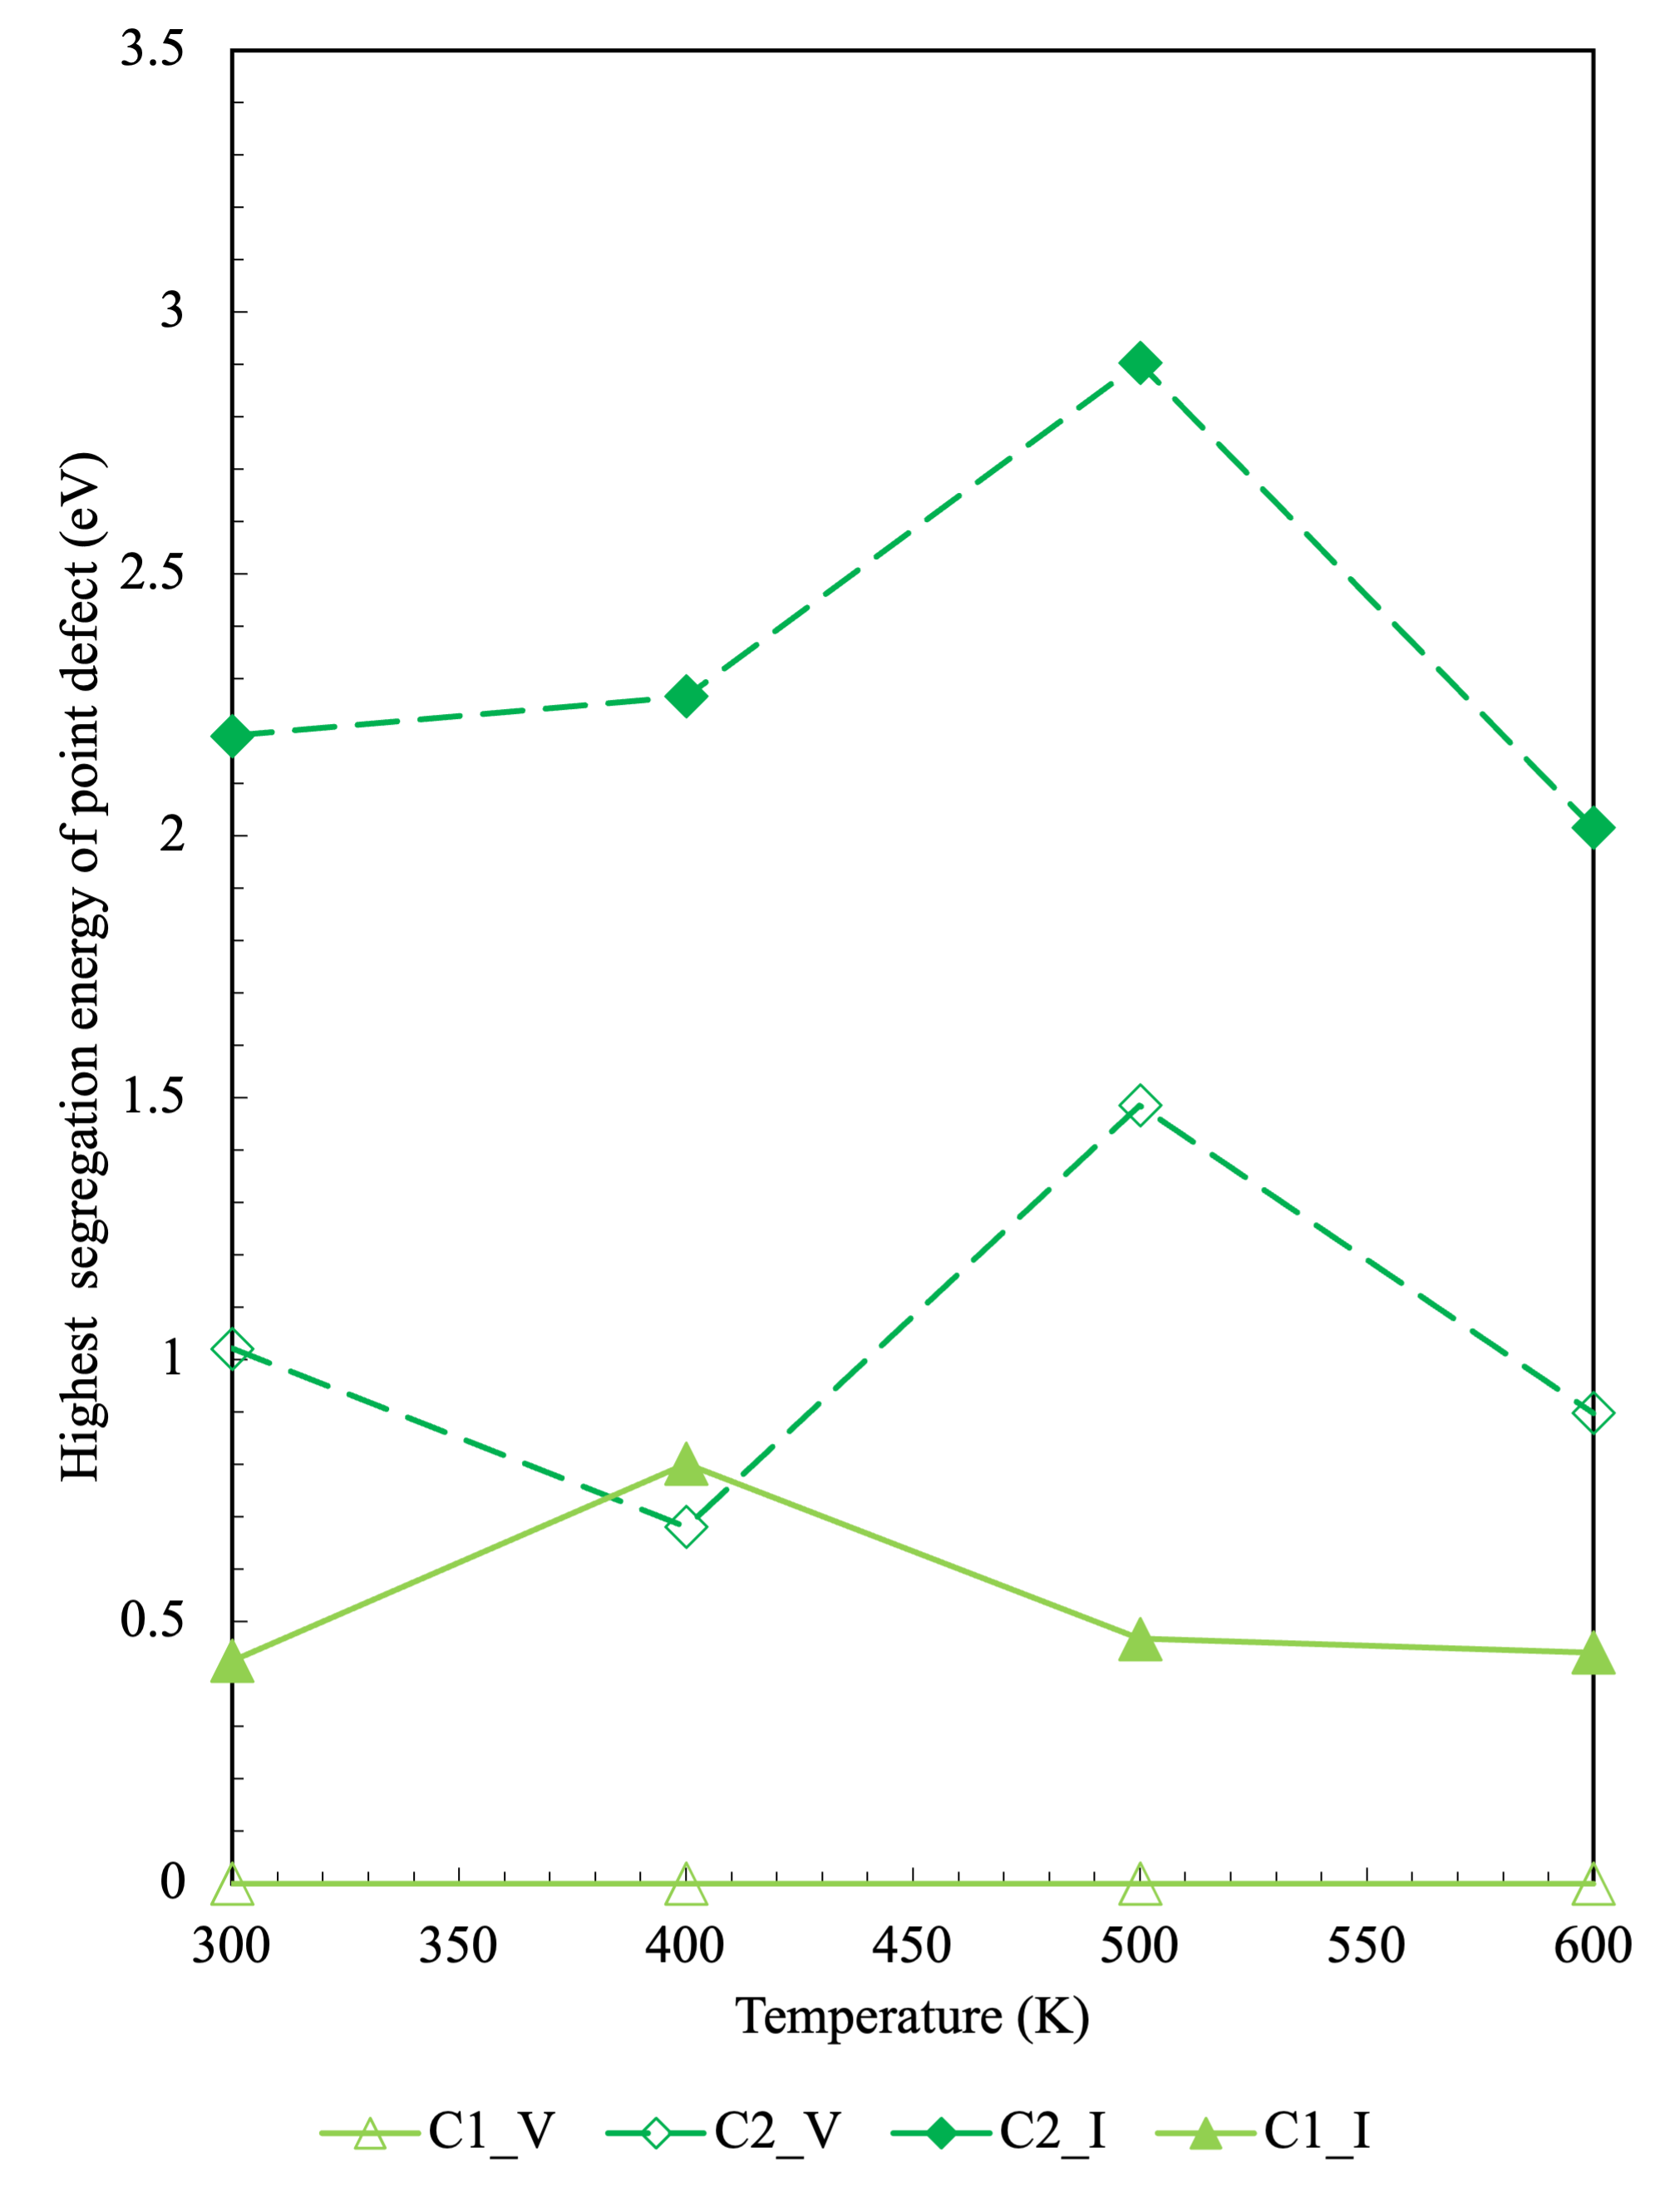
\includegraphics[width = 2.25in]{4_C_SE.png}}\DIFaddendFL \\
\caption{The segregation energy of a point defect as a function of temperature in (a) type A, (b) type B, and (c) type C grain boundaries of $\alpha$-U. In the legend, A1\_V denotes a vacancy within the A1 grain boundary and A1\_I denotes an interstitial within the A1 grain boundary. Solid lines are for low-energy grain boundaries and dashed lines are for high-energy grain boundaries. Open symbols are for vacancies and closed symbols are for interstitials. \DIFaddbeginFL \DIFaddFL{Error bar is not shown for the clarity of the images and error bar has a value of  maximum $\pm$ 0.75 eV.}\DIFaddendFL }
\label{fig:Seg}
\end{figure}

\par The $E_{\mathrm{s}}$ for interstitials is always larger than the $E_{\mathrm{s}}$ of vacancies. For high-energy GBs (A2, B2, C2), the interstitial $E_{\mathrm{s}}$ is approximately twice that of vacancies, while for low-energy GBs, this ratio is even larger (approximately 6 times for B1 at 500 K). Physically, the $E_{\mathrm{s}}$ dictates the tendency of segregation, so an interstitial has a greater tendency to segregate in $\alpha$-U STGBs than a vacancy. In other words, both vacancies and interstitials will be attracted to the grain boundaries, but the grain boundaries are biased sinks with a preference for interstitials.  The general trend of the ratio of the interstitial to vacancy $E_{\mathrm{s}}$ is that it is larger at lower temperatures (300 K) and smaller at elevated temperatures (600 K). Thus, there is a stronger bias for interstitial segregation to grain boundaries at lower temperatures than at higher temperatures. The maximum $E_{\mathrm{s}}$ for a vacancy is observed for the A2 GB at 600 K (1.89 eV), whereas for an interstitial the C2 GB has the maximum value of 2.9 eV at 500 K. STGBs of tungsten also have a bias-absorption effect for interstitials compared with vacancies at 300 K \cite{Tungsten}.  

The $E_{\mathrm{s}}$ is higher for high-energy GBs than for low-energy GBs at a given temperature; that is, high-energy GBs are stronger sinks for point defects than low-energy GBs. For instance, at 500 K the $E_{\mathrm{s}}$ for an interstitial is 7.7 times higher for an A2 GB than for an A1 GB. In the case of type C GBs, the high-energy GB has a 6.2 times higher $E_{\mathrm{s}}$ for an interstitial. Interestingly, most lower energy GBs do not show segregation for vacancies, that is, they do not attract vacancies; as the only lower energy GB that shows segregation for a vacancy is the B1 GB, a similar comparison for vacancies is only valid for type B GBs. For type B GBs, the high-energy GB shows a $E_{\mathrm{s}}$ that is 1.5 times and 4.4 times higher than the low-energy GB for an interstitial and a vacancy, respectively. There is no statistically significant interaction of vacancies with either A1 or C1 GBs. According to GB segregation theory \cite{MISHIN_gb_diff}, when the $E_{\mathrm{s}}$ decreases, the misfit between the point defects and the GB core increases compared to the misfit between point defects and the bulk crystal. As coherent twin boundaries have less atomic misfit, it is expected that the $E_{\mathrm{s}}$ should be lower, that is, it is less energetically favorable to fit an additional atom into a well-ordered grain boundary with little free volume available. These results show that point defect segregation in GBs is more biased for high-energy GBs than low-energy GBs, and indicate that very low formation energy GBs act as poor point defect sinks. This result also supports the results available in the literature, that usually twins and coherent boundaries are not effective sinks for point defects \cite{Nabarro}. Furthermore, this shows that the segregation energy is more strongly dependent upon the  $E_{\mathrm{gb}}$  than on the temperature or even the defect type. Within the studied temperature range, high-energy GBs have on average a 2.5 times higher $E_{\mathrm{s}}$ for interstitials than the low-energy GBs in $\alpha$-U STGBs. For vacancies, the $E_{\mathrm{s}}$ in high-energy GBs is approximately 3 times that of the low-energy GBs.

The average segregation energy of the point defect at the GB core is calculated considering a weighted average depending on GB energies. In this method, the probability of the presence of a GB depends on its formation energy \cite{WILLIAMS201545}. The weighted value of the formation energies of the GBs from the same type (for example, in the case of type A GBs, only the formation energy of GB A1 and A2) are used to determine the weighted-average properties such, as E$_\mathrm{s}$, interaction distance, etc. A similar approach is applied for the type B and type C GBs. This method is noted as the ``weighted average" method for the rest of the article and uses the following equation:
\begin{equation}
\label{eq:weight}
E_{s,x,y}^{WA} = \DIFdelbegin \DIFdel{\frac{E_{gb,1}}{E_{gb,1}+E_{gb,2}} }\DIFdelend \DIFaddbegin \DIFadd{\frac{E_{gb,x}^{1}}{E_{gb,x}^{1}+E_{gb,x}^{2}} }\DIFaddend \times E\DIFdelbegin \DIFdel{_{s,1,y} }\DIFdelend \DIFaddbegin \DIFadd{_{s,y}^{1} }\DIFaddend + \DIFdelbegin \DIFdel{\frac{E_{gb,2}}{E_{gb,1}+E_{gb,2}} }\DIFdelend \DIFaddbegin \DIFadd{\frac{E_{gb,x}^{2}}{E_{gb,x}^{1}+E_{gb,x}^{2}} }\DIFaddend \times E\DIFdelbegin \DIFdel{_{s,2,y}
}\DIFdelend \DIFaddbegin \DIFadd{_{s,y}^{2}
}\DIFaddend \end{equation} 
\noindent where $x$ denotes GB type\DIFdelbegin \DIFdel{and }\DIFdelend \DIFaddbegin \DIFadd{, }\DIFaddend $y$ denotes point defect type \DIFdelbegin \DIFdel{. The $E_{\mathrm{gb}}$ }\DIFdelend \DIFaddbegin \DIFadd{and superscript $1 or 2$ for low and high energy GB. The $E_{\mathrm{gb, x}}^{1 or 2}$ is GB formation energy }\DIFaddend for different types of GBs at different temperatures is taken from Mahbuba \textit{et.al} (2021) \cite{MAHBUBA2021153072}. The results of this method are shown in Fig.~\ref{fig:SE} and indicate that there is no statistically significant difference in the grain boundary types when weighting by the $E_{\mathrm{gb}}$. There is also no dependence on the temperature of the system. Thus, there is an average $E_{\mathrm{gb}}$-weighted vacancy and interstitial segregation energy for $\alpha$-U, which is found to be 0.52 eV and 0.91 eV, respectively. It should be noted that these averaged values are only obtained from a small number of symmetric tilt GBs, and thus may not be representative of a true microstructural average encompassing a wide array of GBs. Non-symmetric tilt GBs are expected to have higher energies than the GBs studied here, and their individual $E_{\mathrm{s}}$ should follow the trends in \Cref{fig:SE_GB}. It is anticipated that the inclusion of such GBs will not affect this weighted average. Thus, this is a reasonable approximation given the trends of segregation energies with respect to orientation that have been observed in this work. 


\begin{figure}[h!]
\centering
\DIFdelbeginFL %DIFDELCMD < \subfloat[]{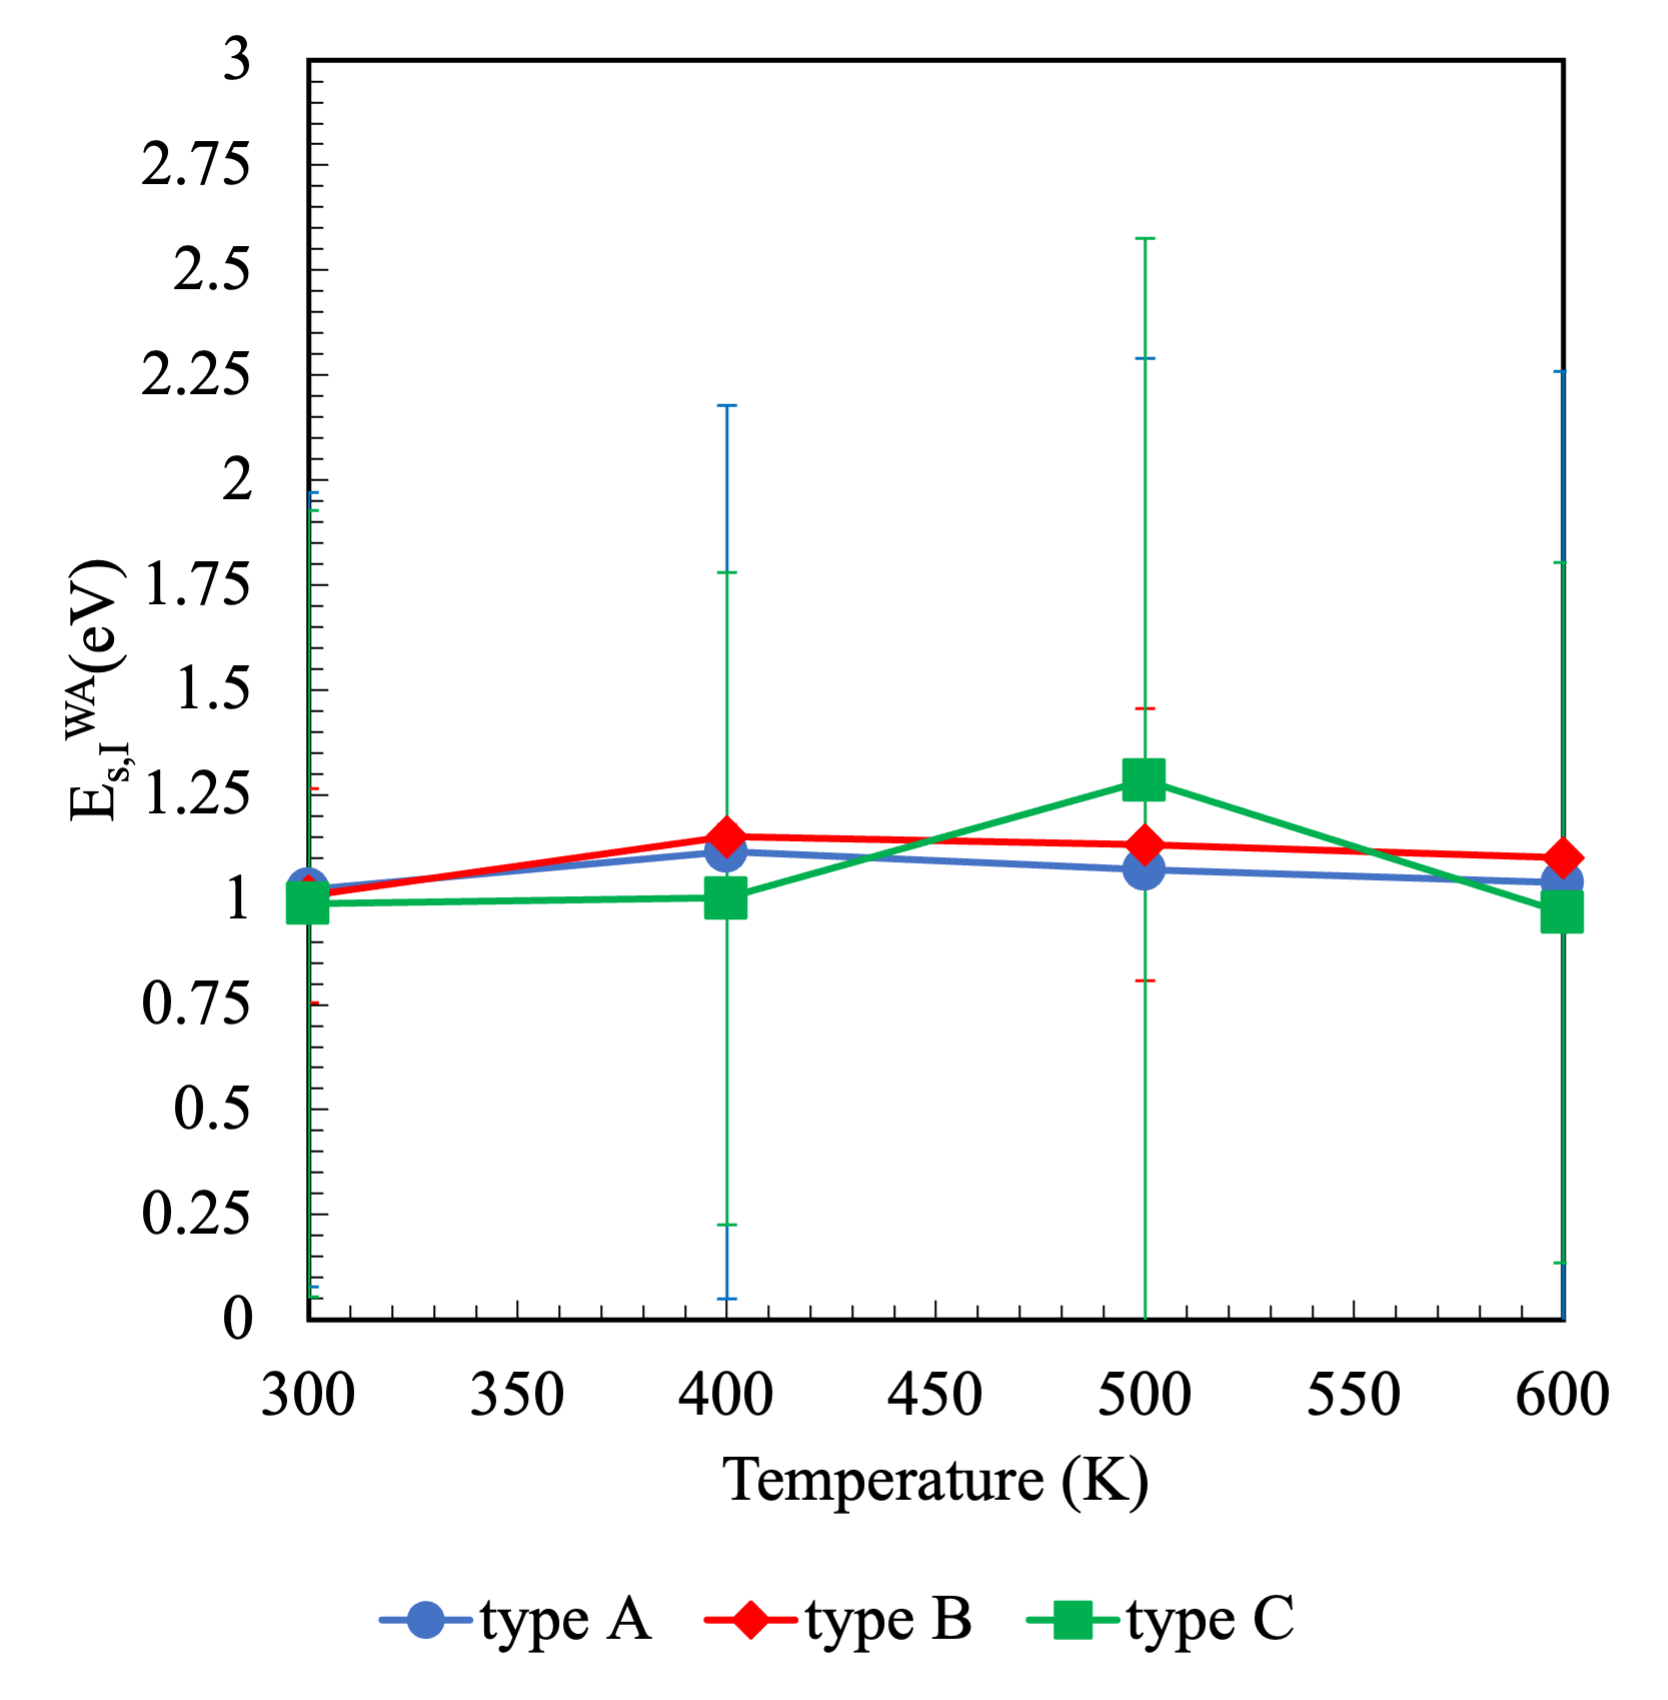
\includegraphics[width = 2.5in]{weighted_SI.png}} 
%DIFDELCMD < \subfloat[]{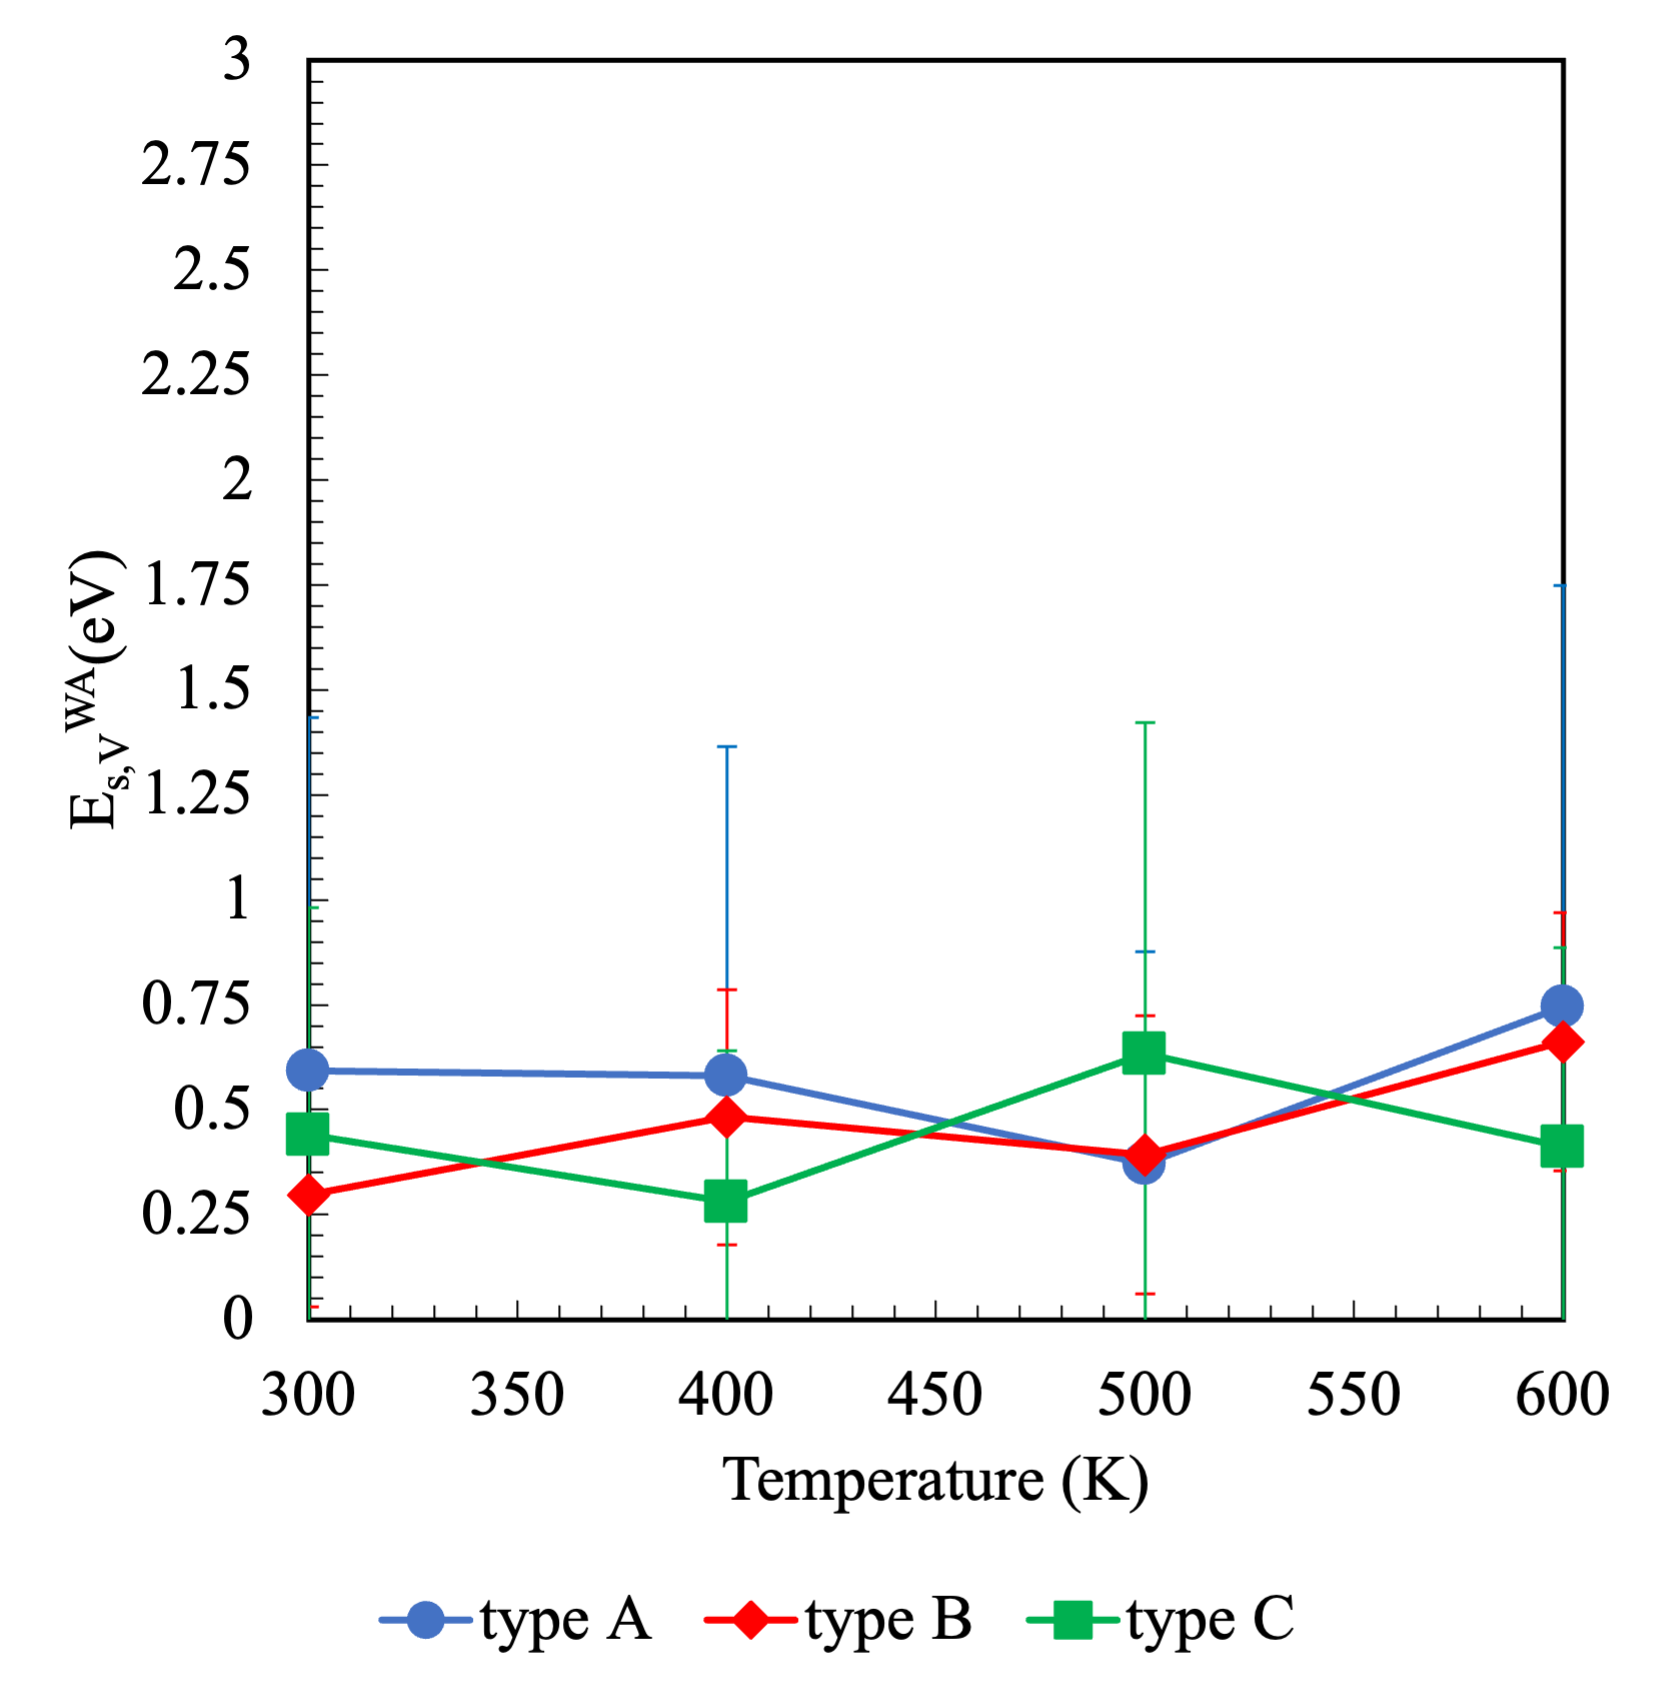
\includegraphics[width = 2.5in]{weighted_SV.png}}
%DIFDELCMD < %%%
\DIFdelendFL \DIFaddbeginFL \subfloat[]{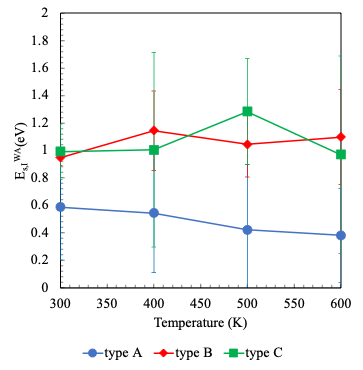
\includegraphics[width = 2.5in]{5_weighted_SI.png}} 
\subfloat[]{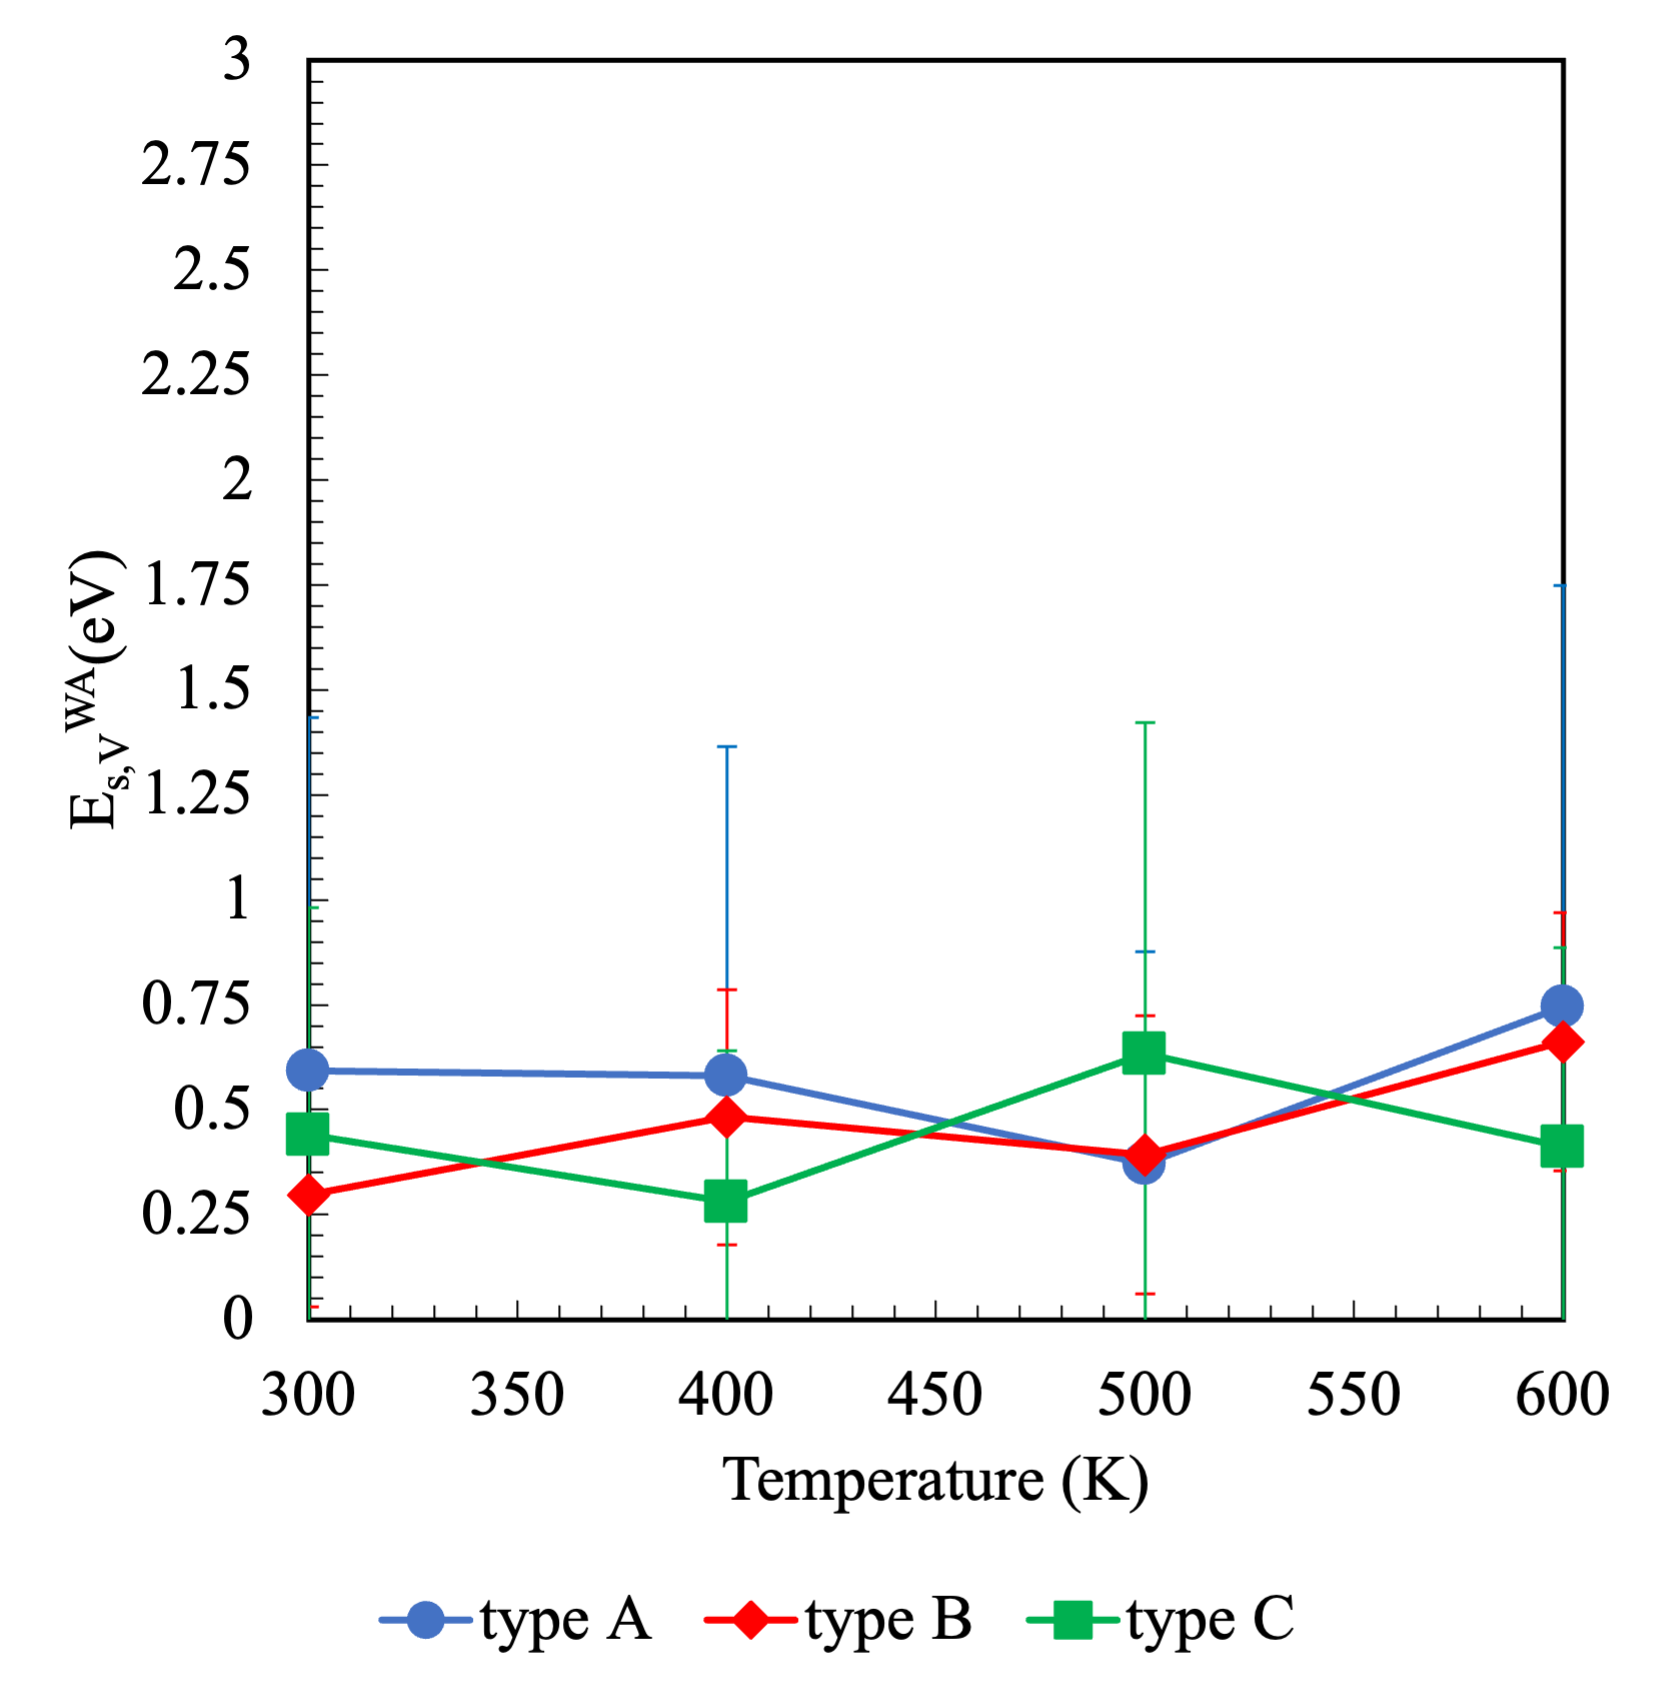
\includegraphics[width = 2.5in]{5_weighted_SV.png}}
\DIFaddendFL \caption{(a) Weighted average segregation energy in $\alpha$-U with (a) interstitial and (b) vacancy plotted over temperature. Error bars in these figures are the propagated standard error. }
\label{fig:SE}
\end{figure}


\DIFdelbegin %DIFDELCMD < \par %%%
\DIFdel{Segregation energies ($E_{\mathrm{s}}$) at all temperatures for all studied GBs are plotted with respect to the corresponding  $E_{\mathrm{gb}}$  in \Cref{fig:SE_GB}. Data for interstitials and vacancies can be separately fitted by a linear function. The $E_{\mathrm{s}}$ increases with  $E_{\mathrm{gb}}$  at a rate of 2.99 eV per $J/m{^2}$ for interstitials and 2.92 eV per $J/m^2$ for vacancies. Though both of the point defect types have similar rates of increase, there is a threshold value in $E_{\mathrm{gb}}$ for vacancy segregation which is about 0.4 $J/m^2$. An MD study on $\alpha$-Fe for both tilt and twist GBs showed a linear relationship of point defect $E_{\mathrm{s}}$ with $E_{\mathrm{gb}}$ \cite{tschopp2012probing}, essentially confirming the results here, albeit in a different material and with different functional slopes. 
}%DIFDELCMD < 

%DIFDELCMD < \begin{figure}[h!]
%DIFDELCMD < \centering
%DIFDELCMD < 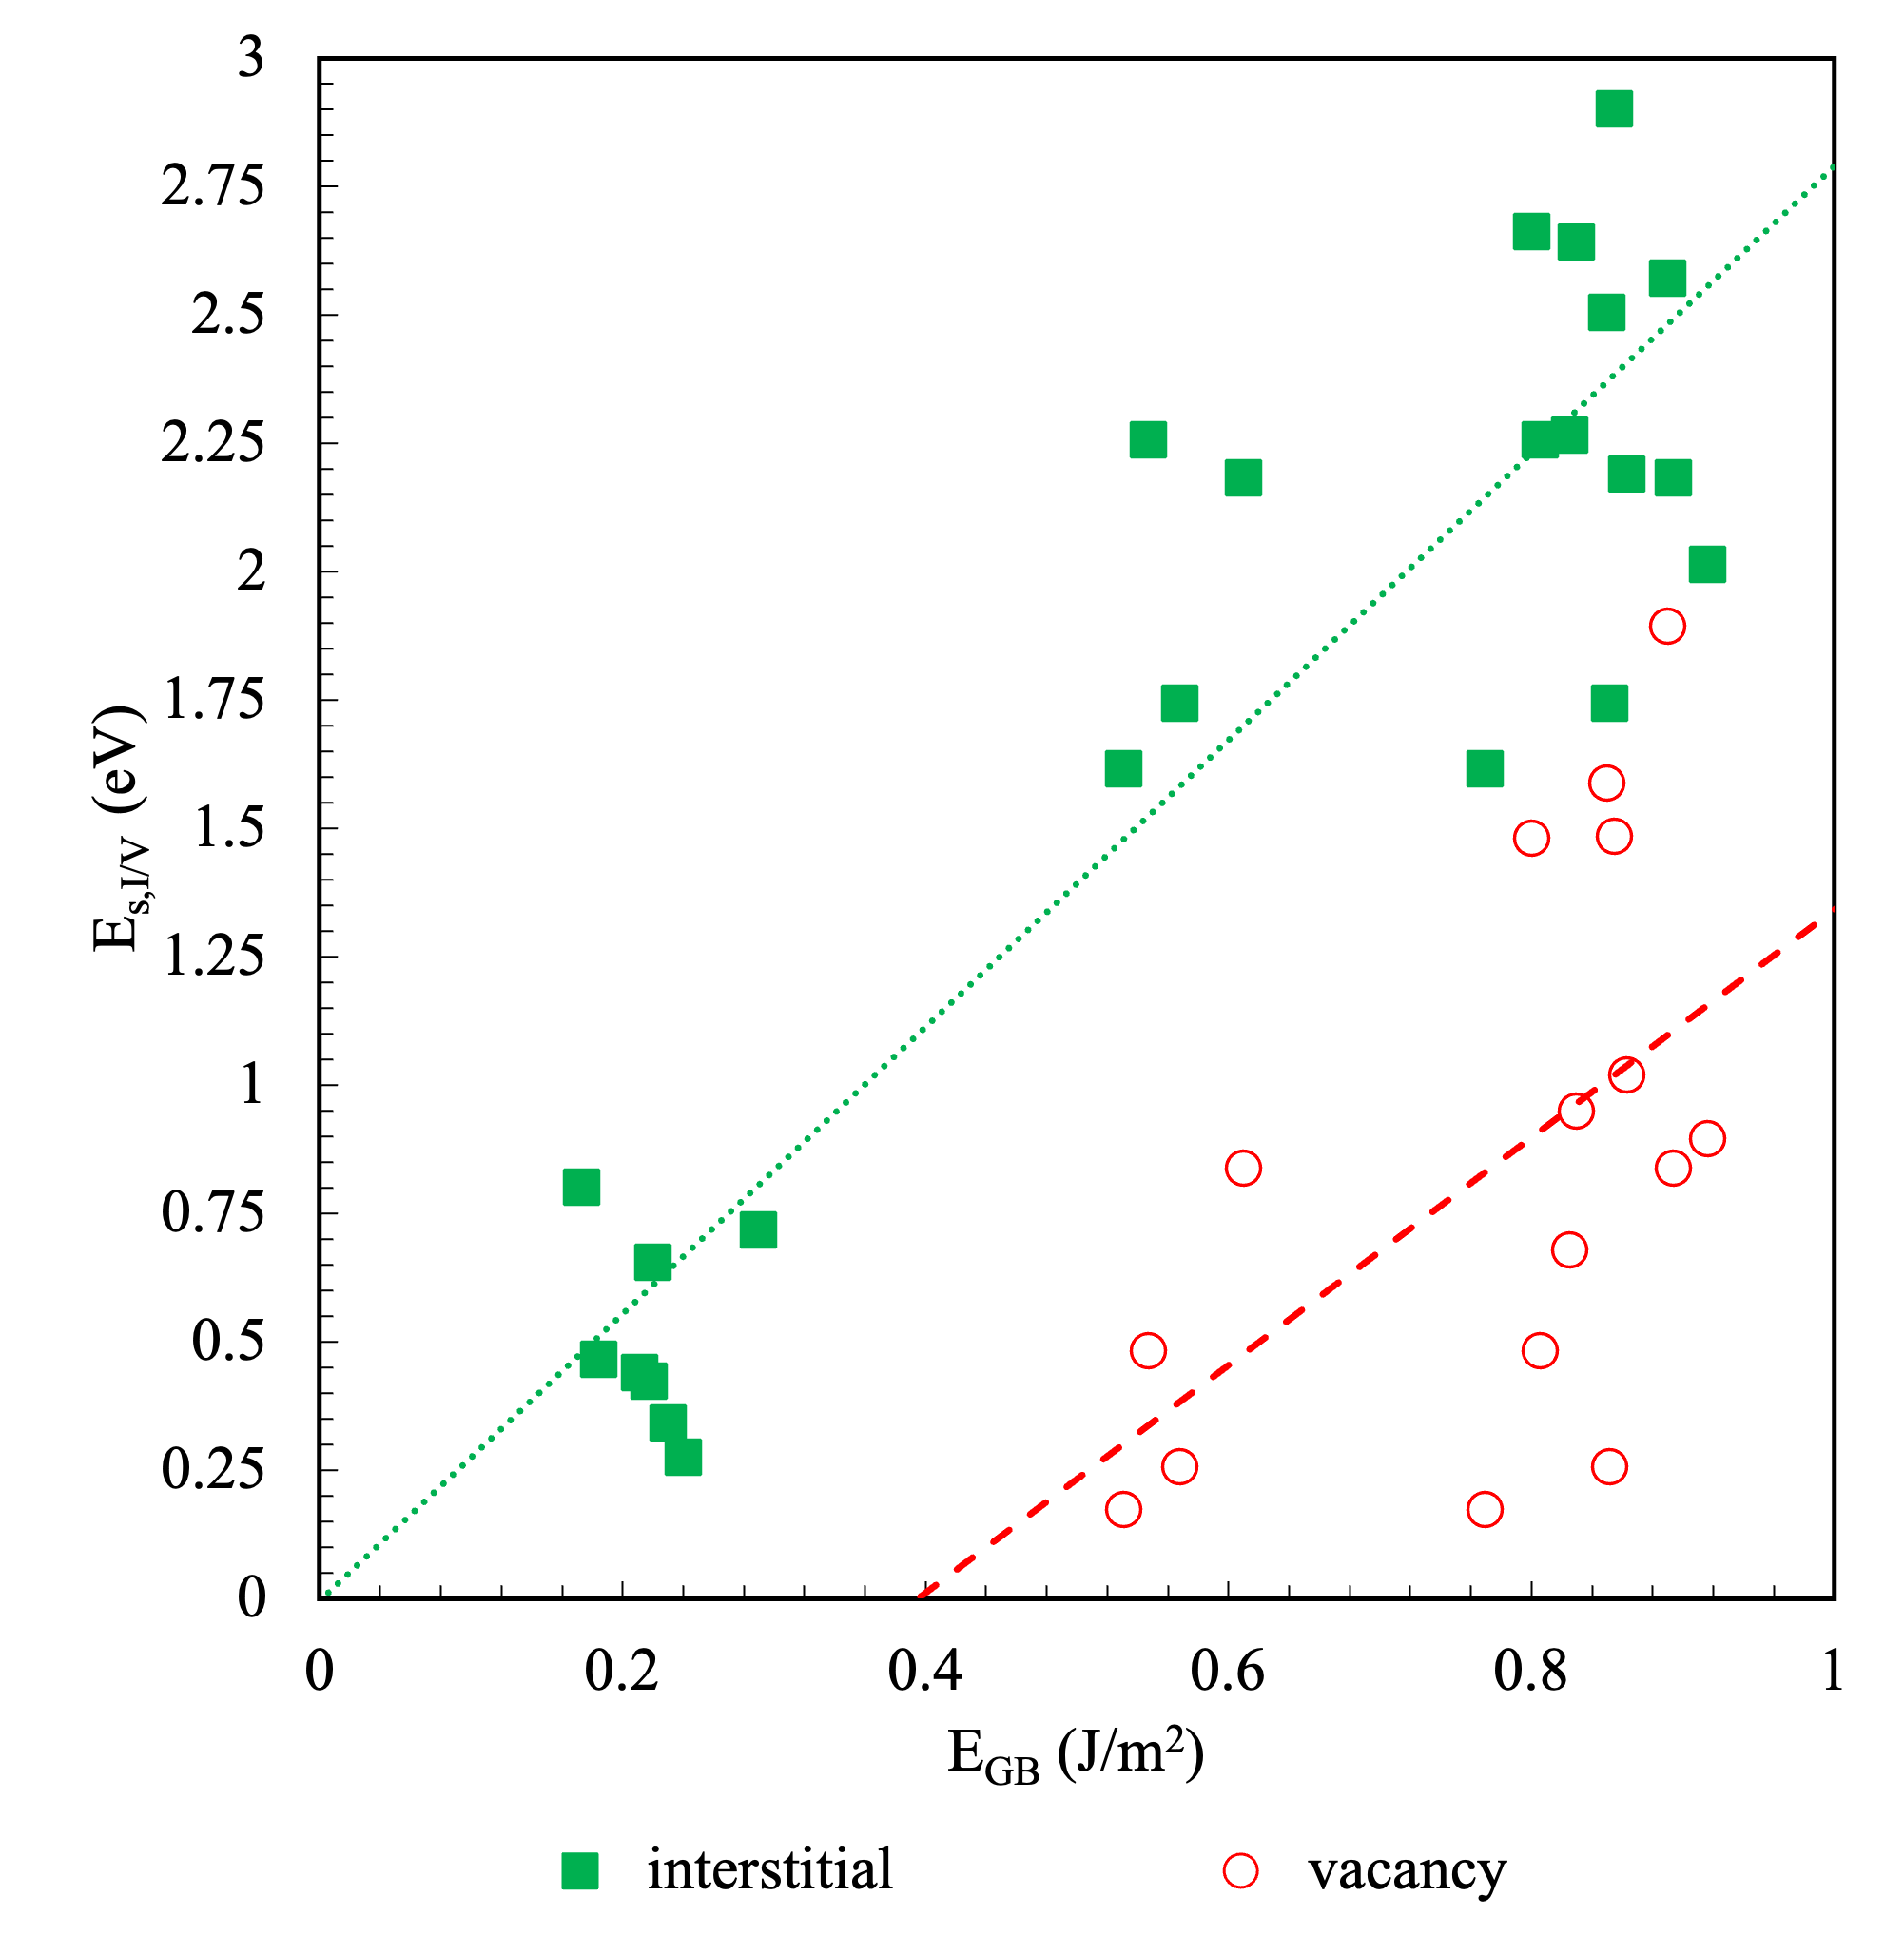
\includegraphics[width = 3in]{SE_GB.png}\\
%DIFDELCMD < %%%
%DIFDELCMD < \caption{%
{%DIFAUXCMD
\DIFdelFL{Segregation energy of point defects at GBs in $\alpha$-U at different studied temperatures plotted as a function of the corresponding $E_{\mathrm{gb}}$.}}
%DIFAUXCMD
%DIFDELCMD < \label{fig:SE_GB}
%DIFDELCMD < \end{figure}
%DIFDELCMD < 

%DIFDELCMD < %%%
\DIFdelend \FloatBarrier

\subsubsection{Interaction Lengths}
\par A parameter related to the $E_{\mathrm{s}}$ is the  $l_{\mathrm{int}}$ of a point defect with the GB. This length is the distance at which the $E_{\mathrm{s}}$ becomes zero, which dictates up to what distance there is a tendency for point defects to segregate into the GB. As the studied system has symmetries along the tilt axis, the $l_{\mathrm{int}}$ reported here should be doubled when used in larger length-scale modeling. In \Cref{fig:Int}, the interaction length is plotted as a function of temperature. One general trend observed for all GB types is that an interstitial exhibits a larger  $l_{\mathrm{int}}$ from the GB core than a vacancy, with a ratio of up to 2.4 times greater for the high-energy GBs (A2, B2, and C2). Among the studied GBs, the maximum  $l_{\mathrm{int}}$ of 23~{\AA} is observed for the B1 GB at 600 K (considering all temperatures). Type A GBs have relatively smaller interaction lengths than type C and B. 

\begin{figure}[h!]
\centering
\DIFdelbeginFL %DIFDELCMD < \subfloat[]{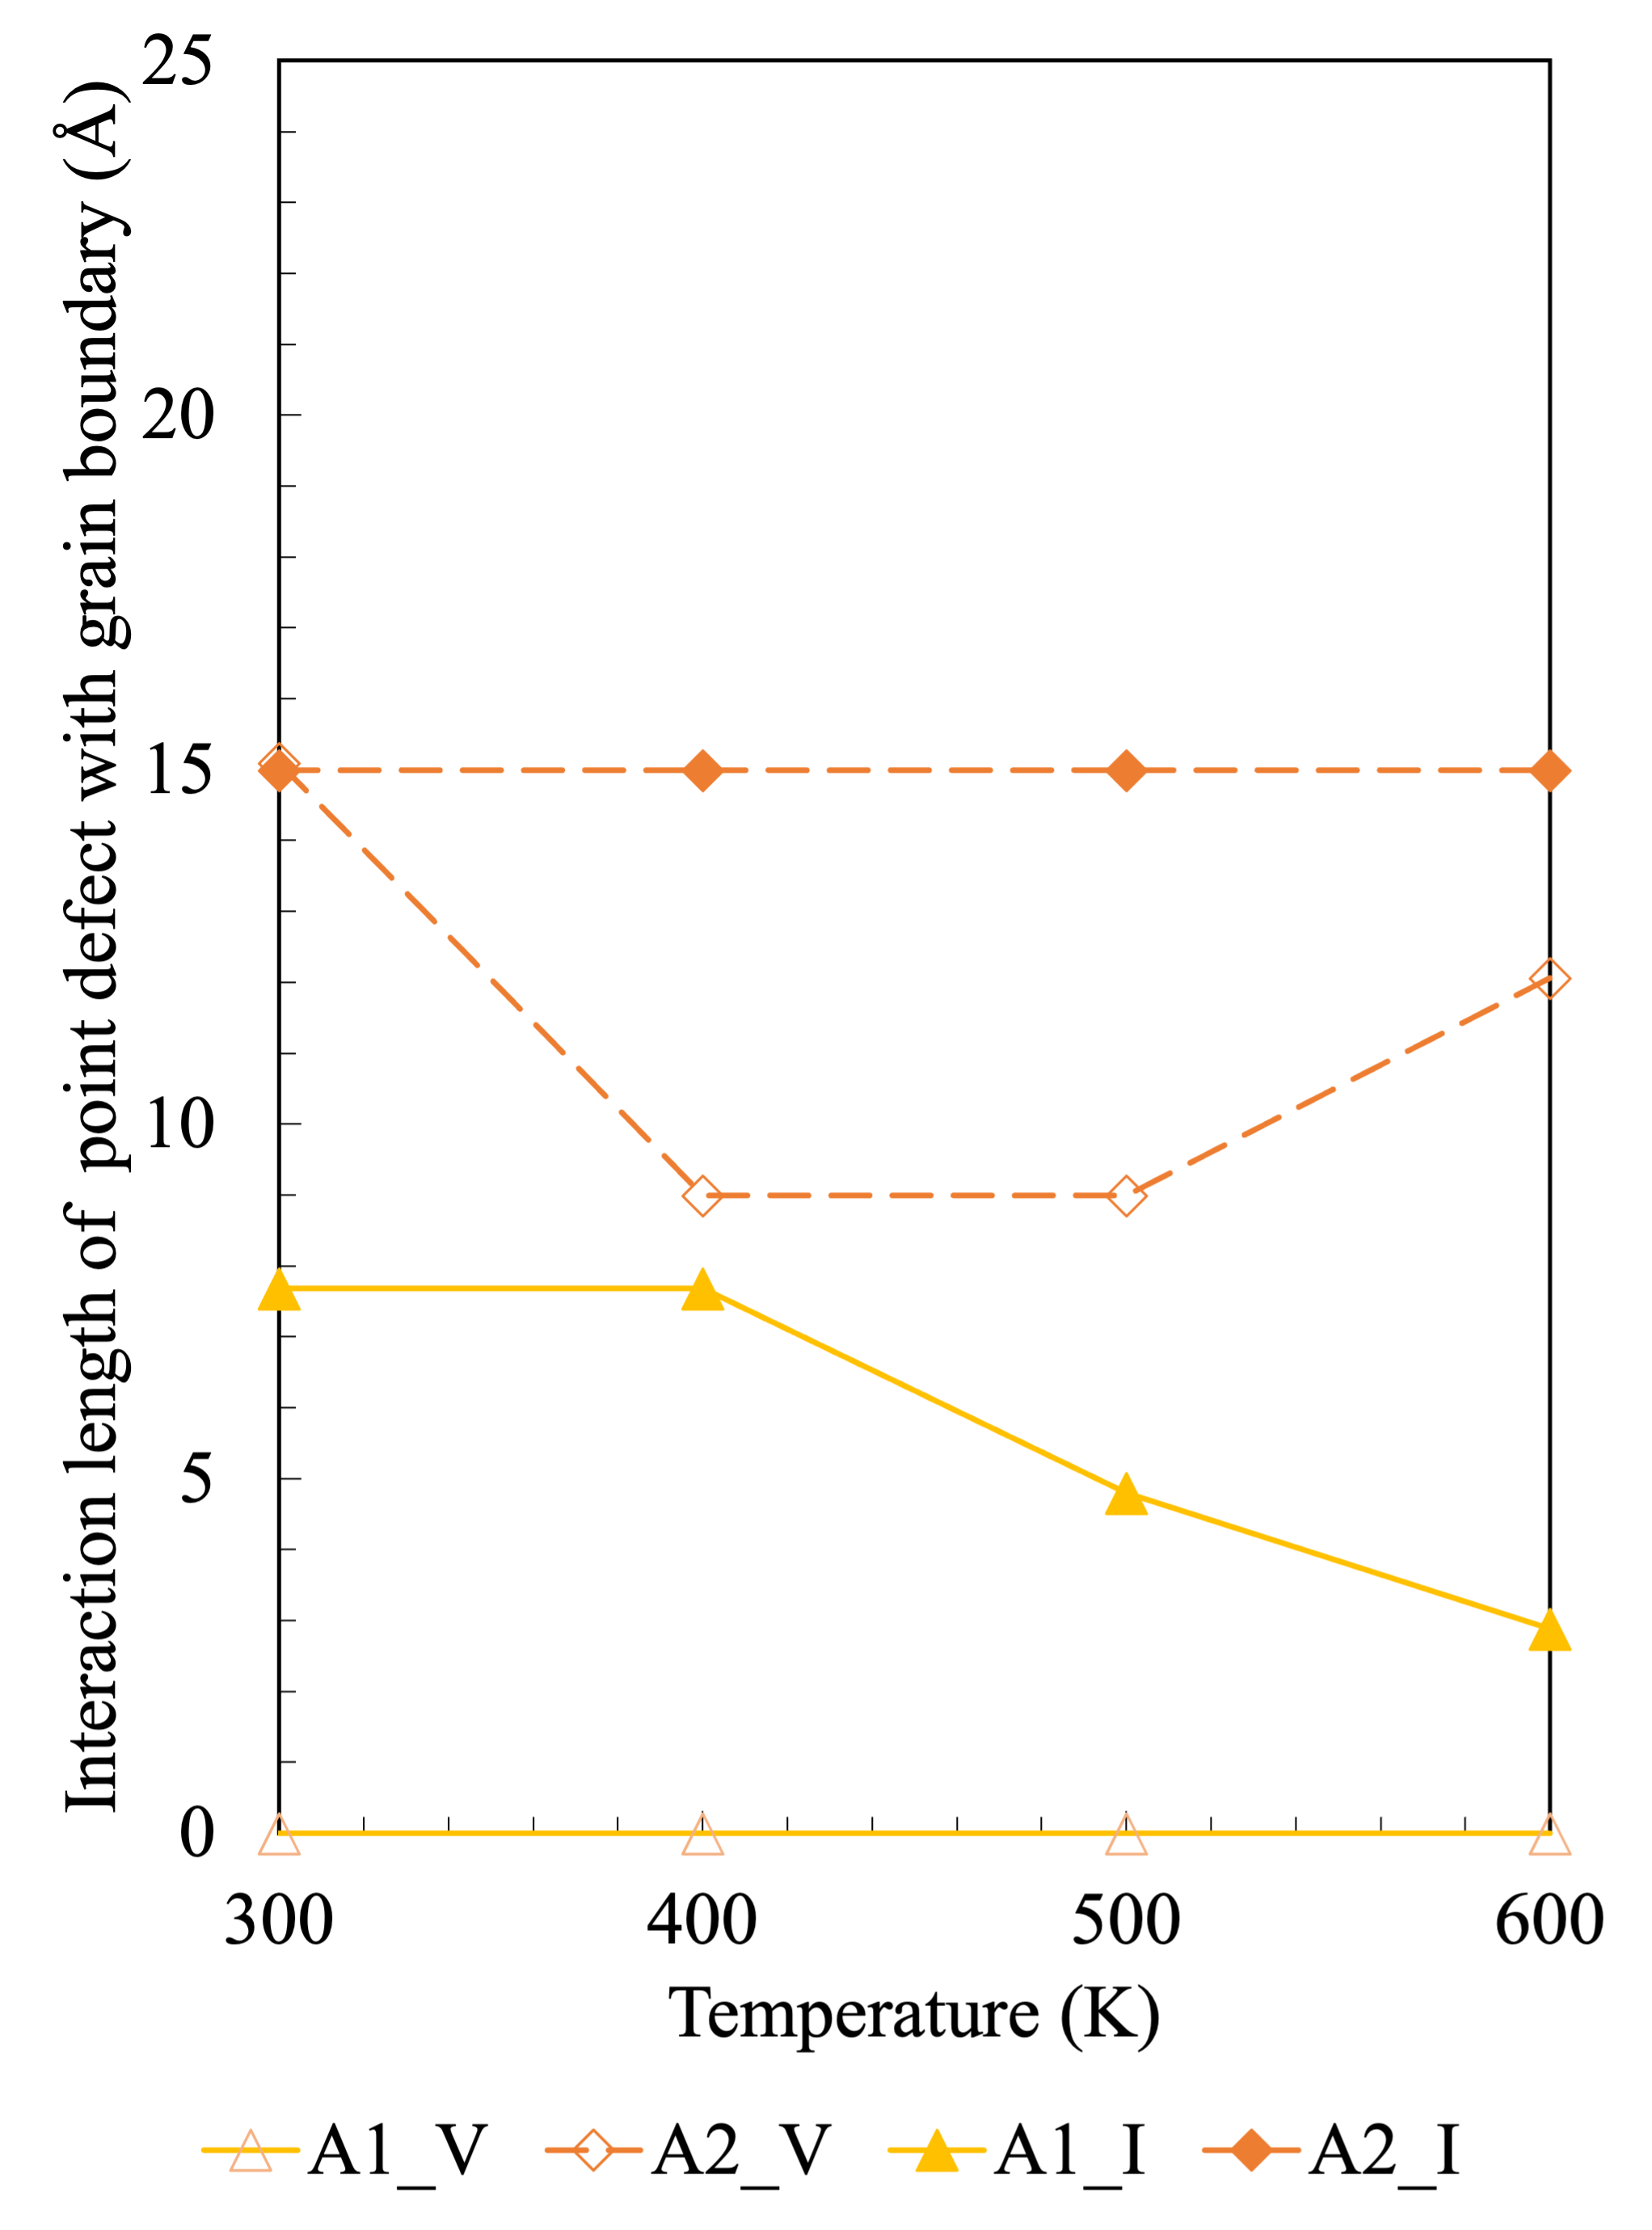
\includegraphics[width = 2.25in]{A_IL.png}}
%DIFDELCMD < \subfloat[]{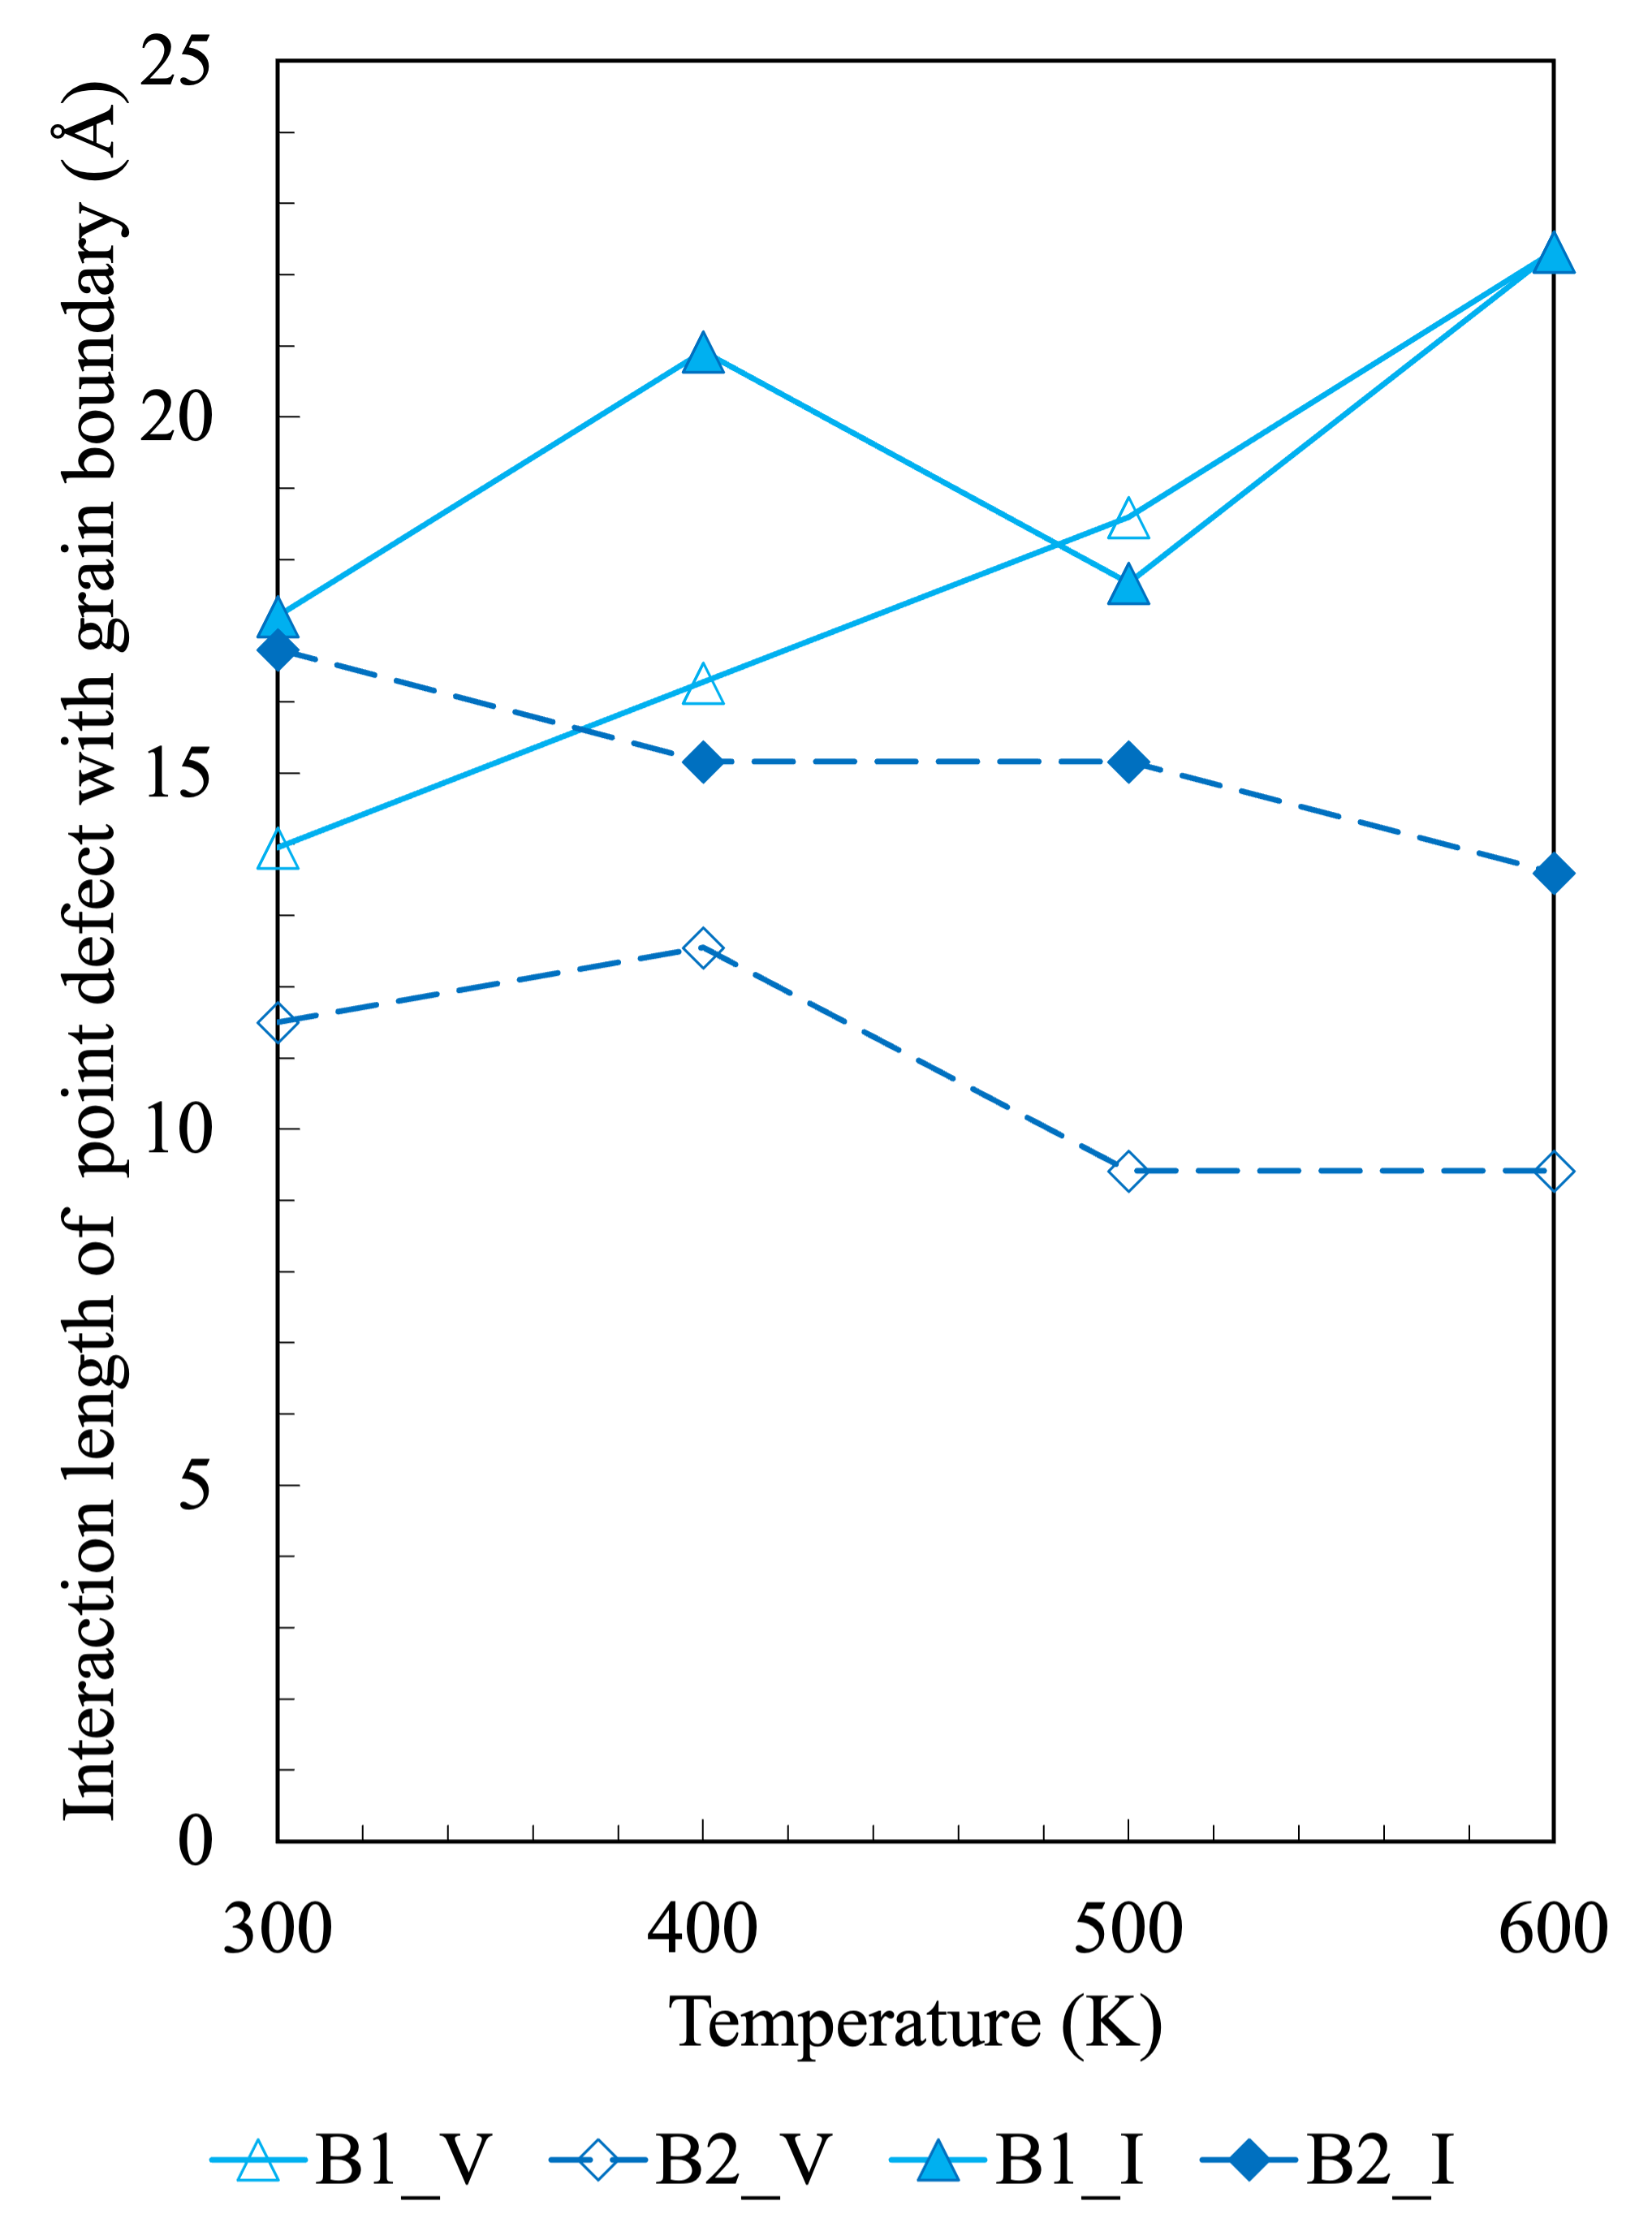
\includegraphics[width = 2.25in]{B_IL.png}} 
%DIFDELCMD < \subfloat[]{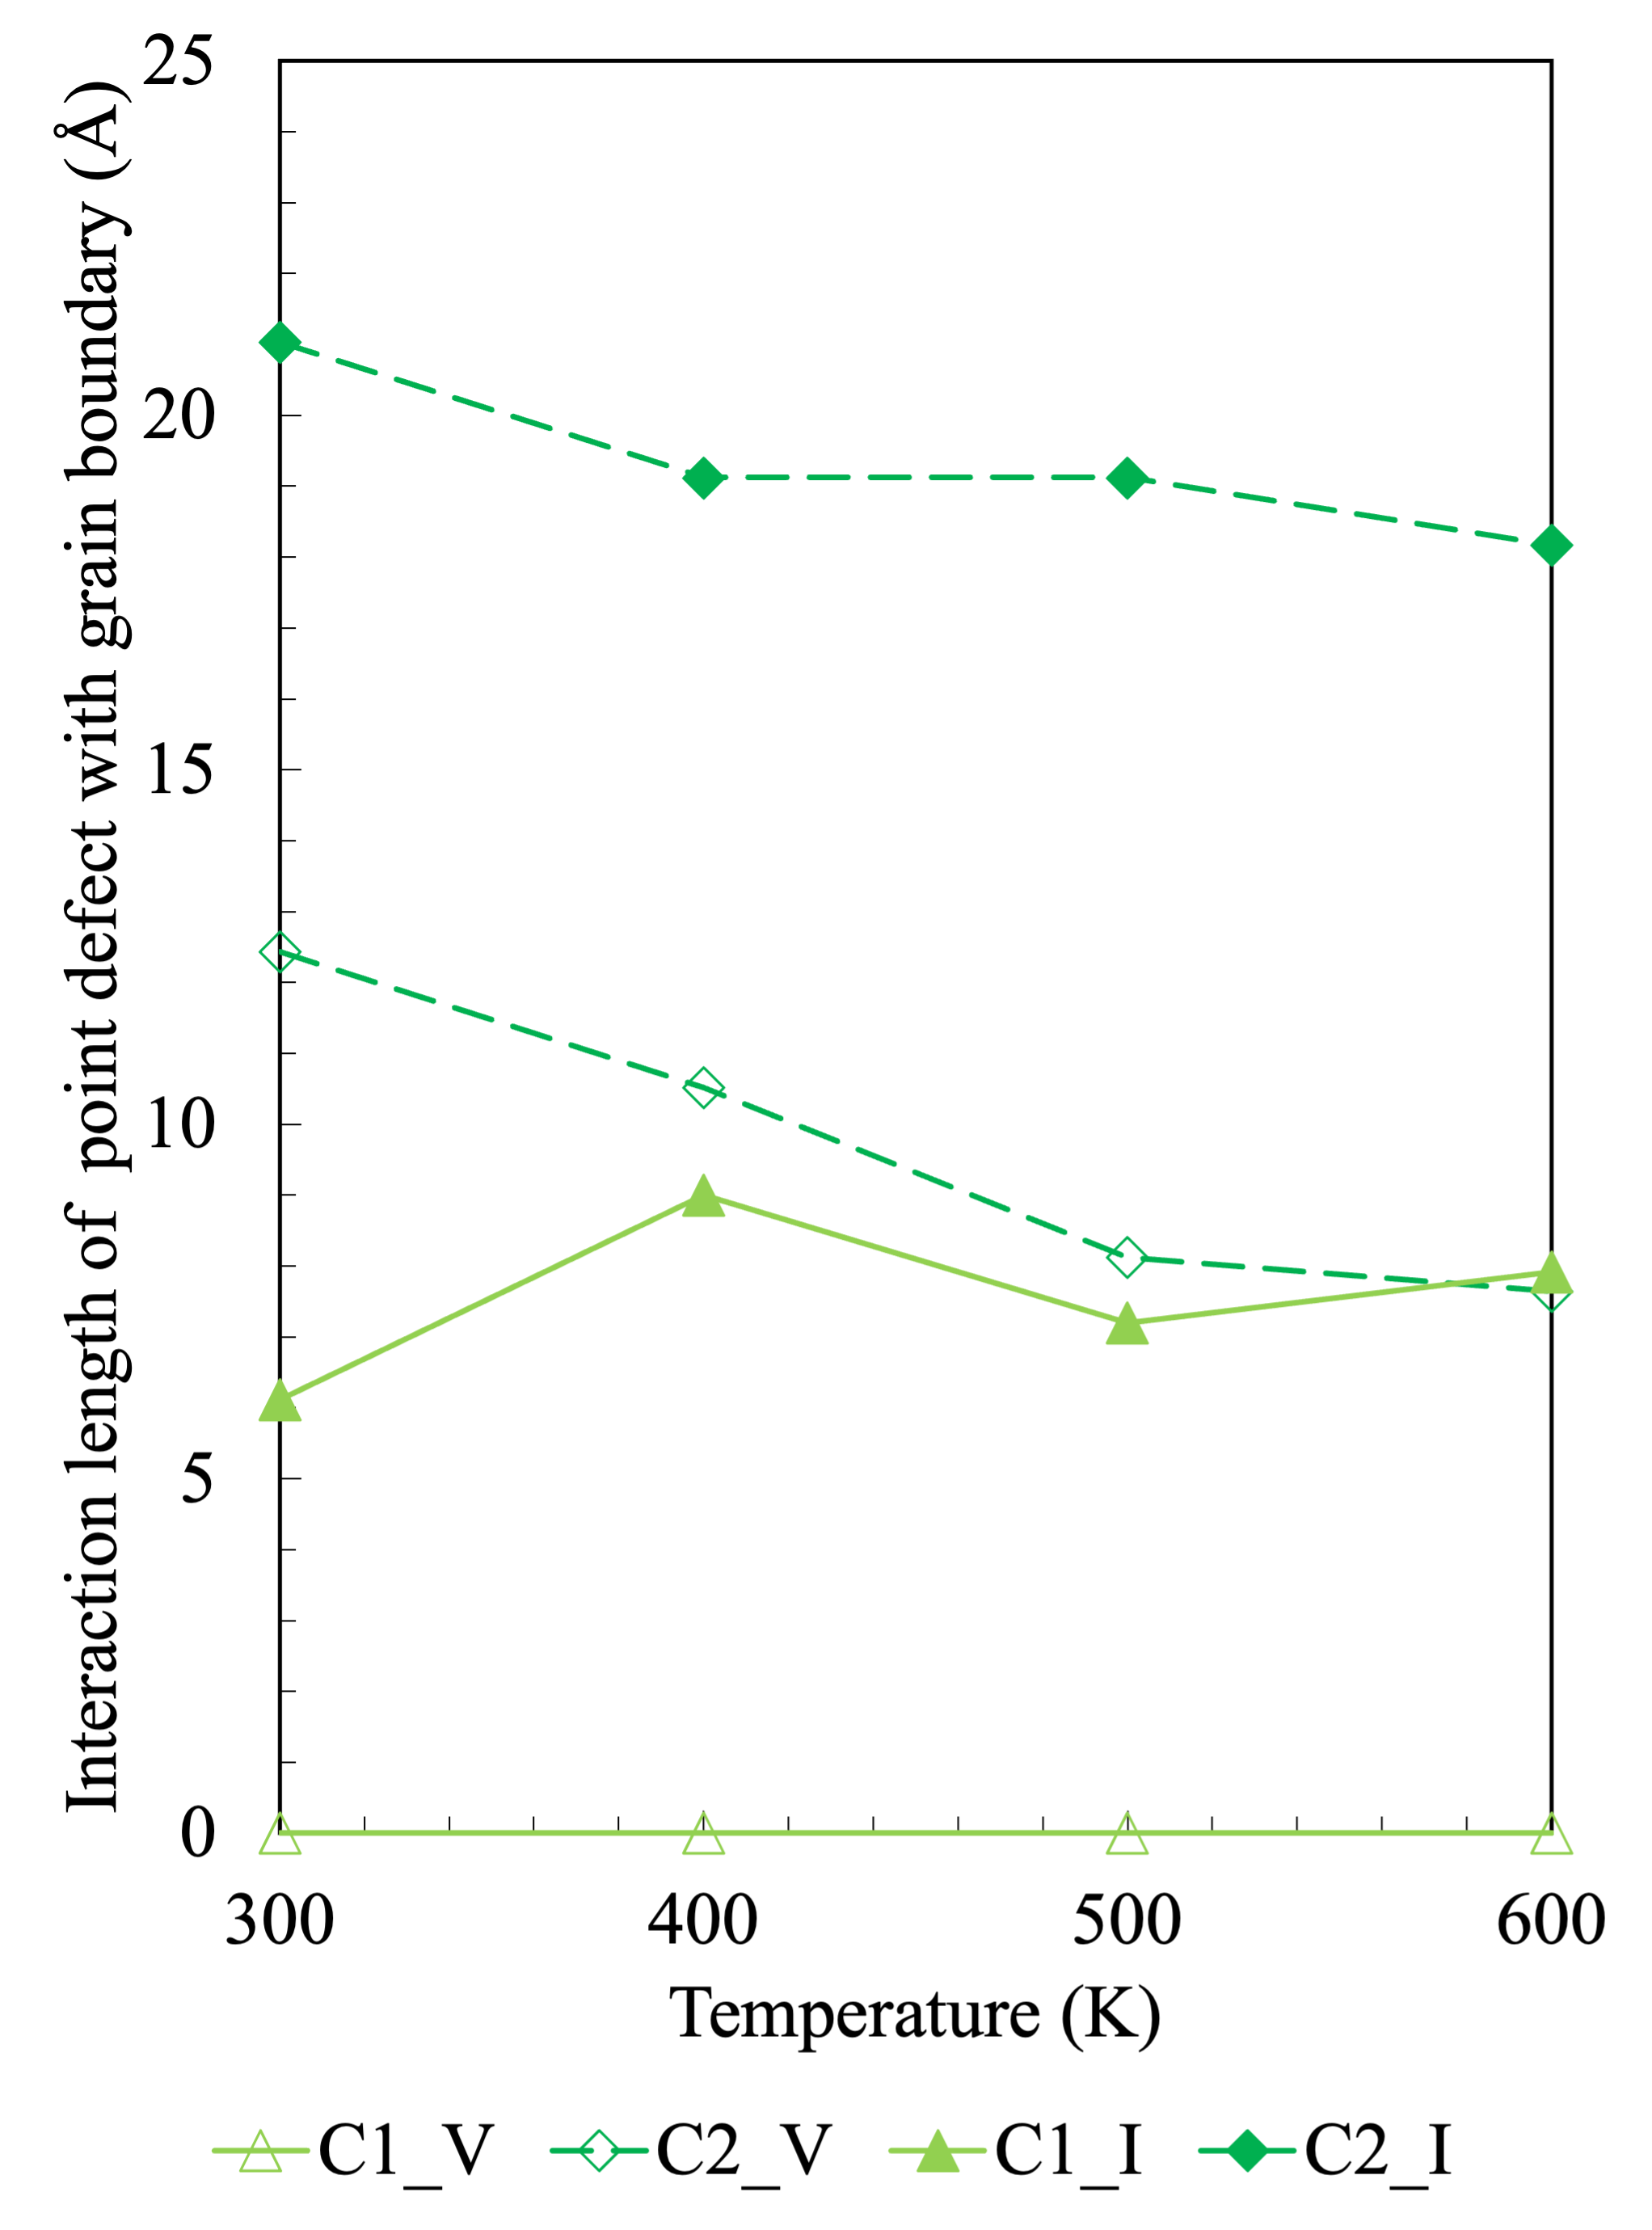
\includegraphics[width = 2.25in]{C_IL.png}}%%%
\DIFdelendFL \DIFaddbeginFL \subfloat[]{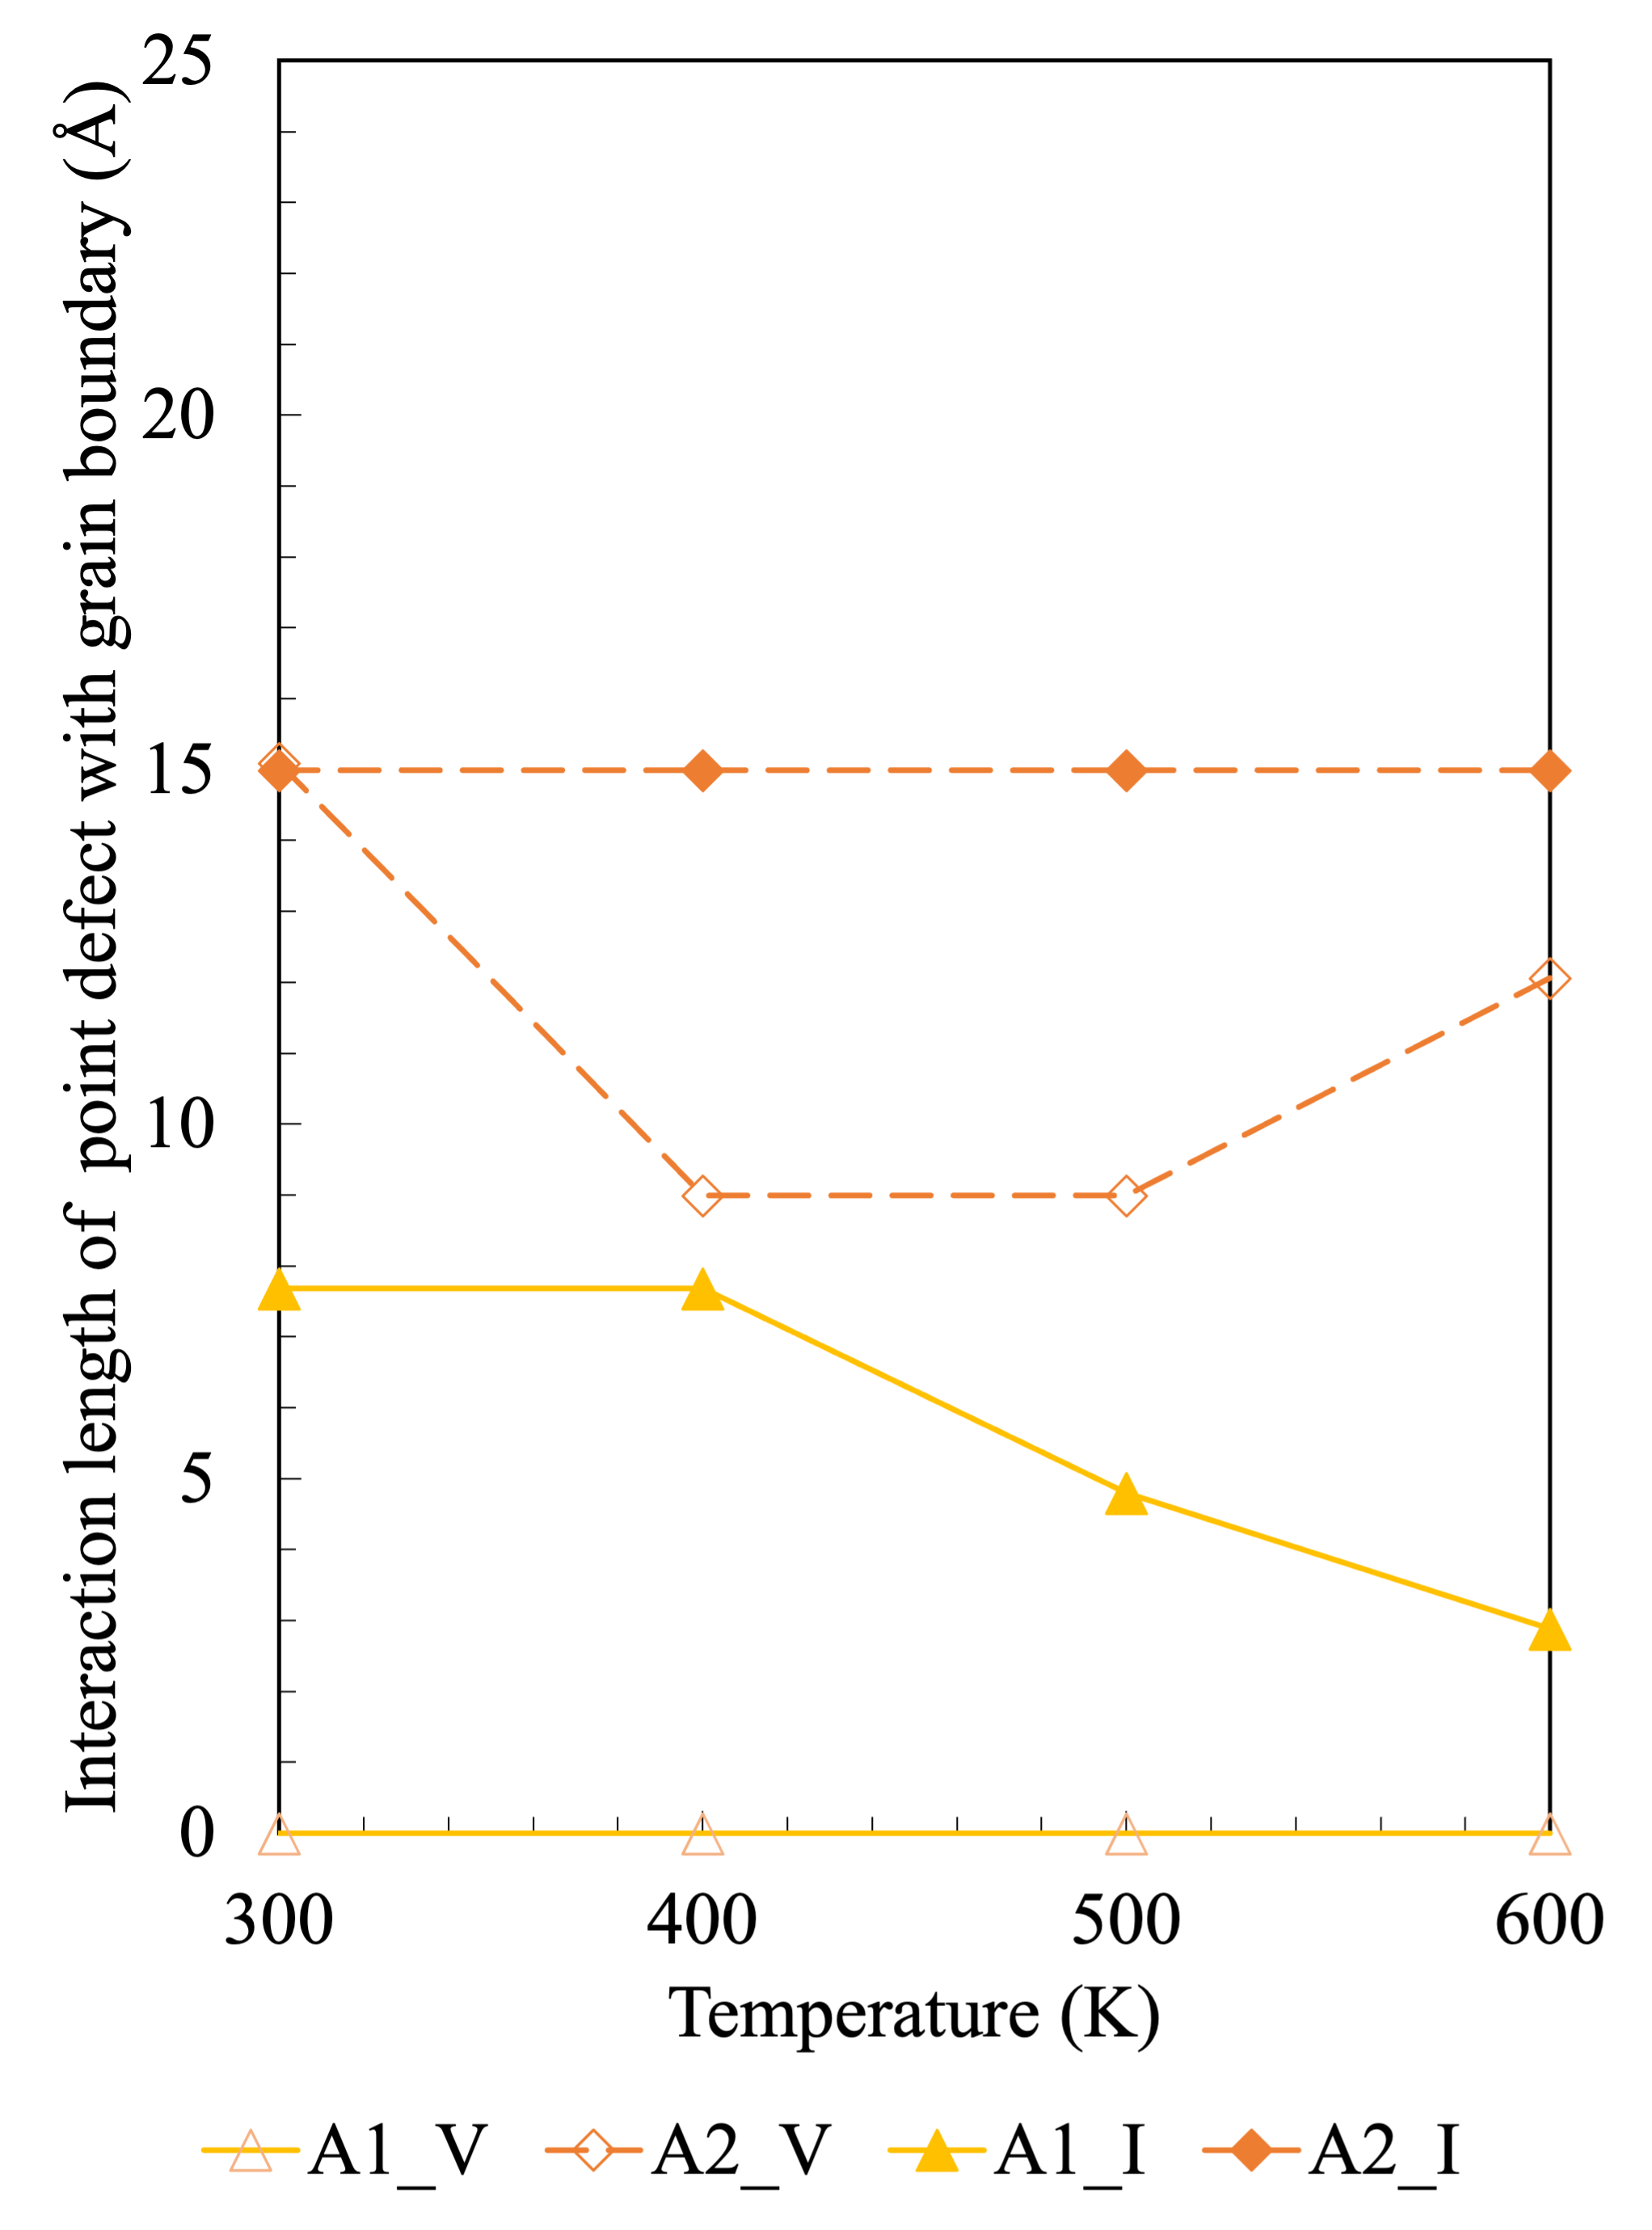
\includegraphics[width = 2.25in]{6_A_IL.png}}
\subfloat[]{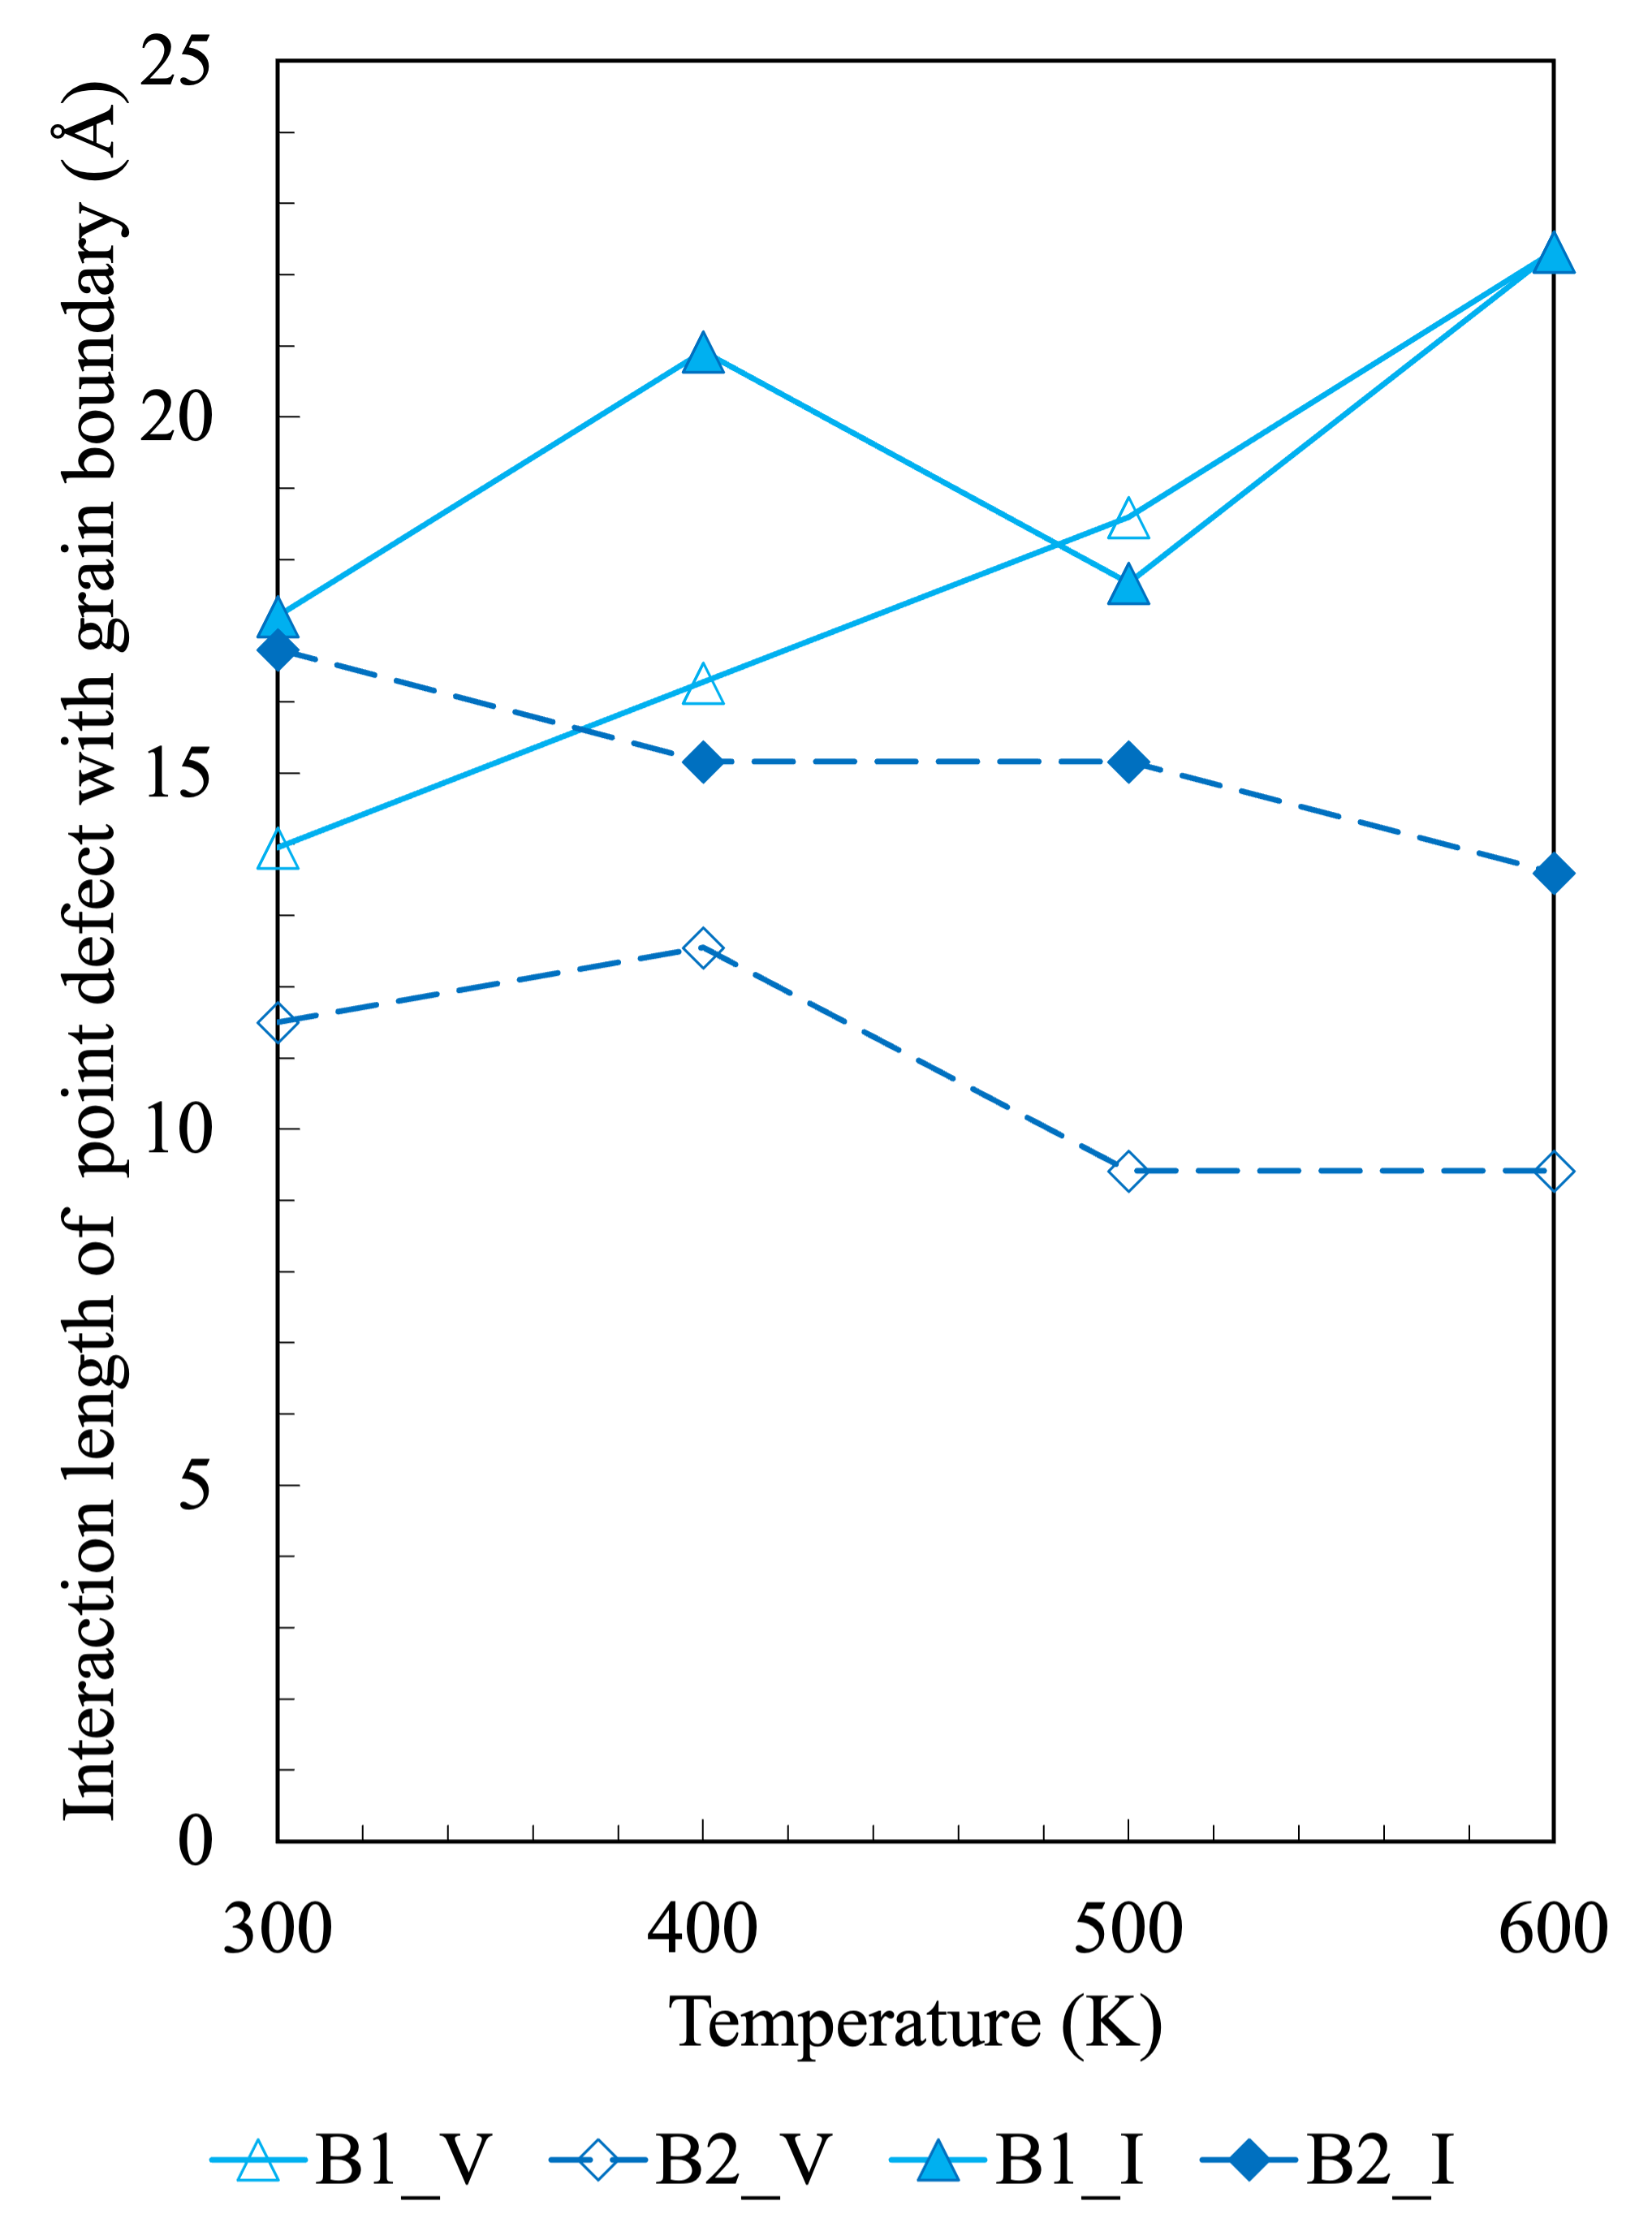
\includegraphics[width = 2.25in]{6_B_IL.png}} 
\subfloat[]{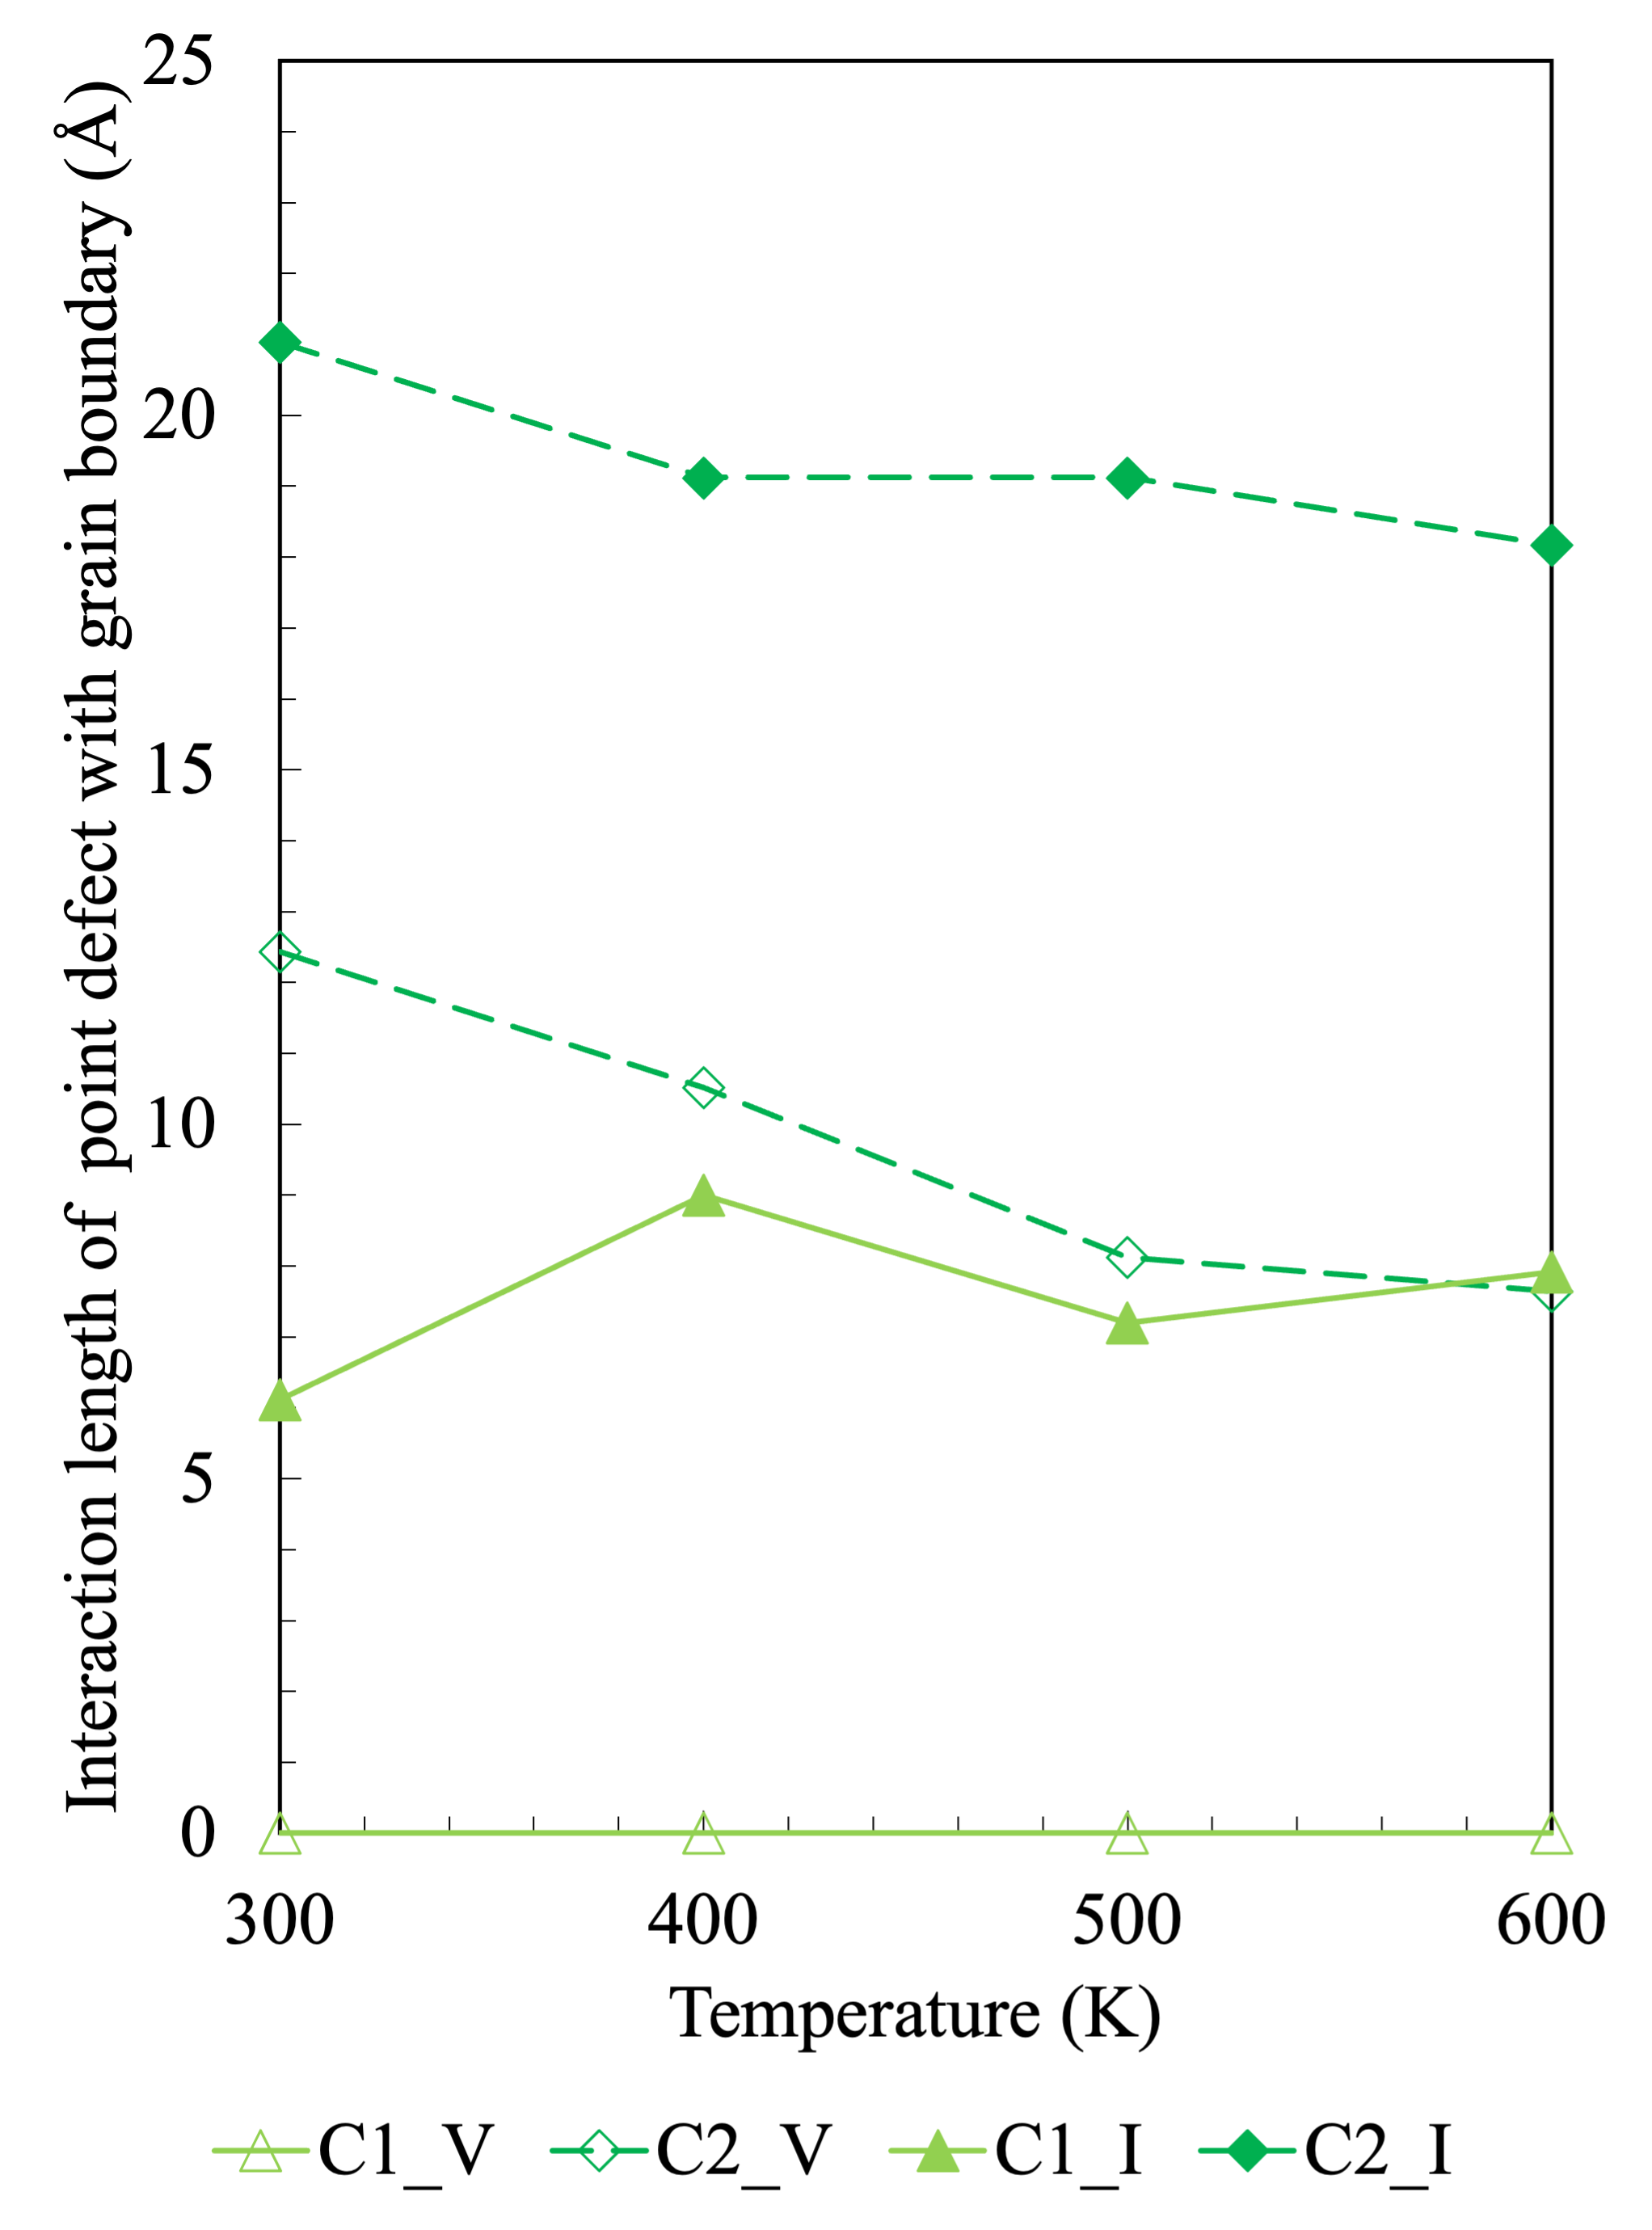
\includegraphics[width = 2.25in]{6_C_IL.png}}\DIFaddendFL \\
\caption{Interaction length of a point defect as a function of temperature due to the presence of (a) type A, (b) type B, and (c) type C grain boundaries of $\alpha$-U. In the legend, A1\_V means the interaction length between a vacancy and the A1 grain boundary, and A1\_I means the interaction length between an interstitial and the A1 grain boundary. Solid lines are for low-energy grain boundaries and dashed lines are for high-energy grain boundaries. Open symbols are for vacancies and closed symbols are for interstitials.}
\label{fig:Int}
\end{figure}

\par The low-energy A1 and C1 GBs only show an interaction with interstitials, not with vacancies. The $l_{\mathrm{int}}$ of an interstitial for these two GBs is one order of magnitude lower than the other GBs. For the A1 GB, the  $l_{\mathrm{int}}$ ranges between 2.9 - 7.7 {\AA}, and the  $l_{\mathrm{int}}$ varies between 6.1 - 9.0 {\AA} for the C1 GB. The other low-energy GB considered in the current work, B1, interacts with both vacancies and interstitials. There are mixed trends regarding the  $l_{\mathrm{int}}$ as a function of temperature. The B1 GB tends to see an increase in  $l_{\mathrm{int}}$ with temperature, while the $l_{\mathrm{int}}$ for A1 and C2 tend to decrease with temperature. Overall, the change in both $E_{\mathrm{s}}$ and  $l_{\mathrm{int}}$ of point defects with temperature is likely statistically insignificant. Finally, high-energy GBs have on average a 1.5 times longer $l_{\mathrm{int}}$ for interstitials than the low-energy GBs in $\alpha$-U.



\par Using the same weighted averaging technique considered for $E_{\mathrm{s}}$ of point defects, the weighted average $l_{\mathrm{int}}$ of a vacancy and an interstitial is determined, and the data is plotted in figure \Cref{fig:IL}. Once again there is no discernible difference in the  $l_{\mathrm{int}}$ as a function of temperature. However, there does appear to be a minor difference between GB types. Shorter interaction lengths are observed for Type A GBs with interstitials, while longer ILs are observed for Type B GBs with vacancies. However, the differences in the $l_{\mathrm{int}}$ of different GB types are not statistically significant, and thus we report a single energy-weighted value of the $l_{\mathrm{int}}$ for interstitials and vacancies of 7.8 {\AA} and 5 {\AA}, respectively. As stated previously, when using the average interaction length of $\alpha$-U GBs at larger length scales, the values reported here should be doubled. After doubling, the $l_{\mathrm{int}}$ for interstitials and vacancies are 15.6 {\AA} and 10 {\AA}, respectively, slightly smaller than the $l_{\mathrm{sb}}$ (related to the GB structure as mentioned in \ref{sec:comp2}). 


\begin{figure}[h!]
\centering
%DIF < \subfloat[]{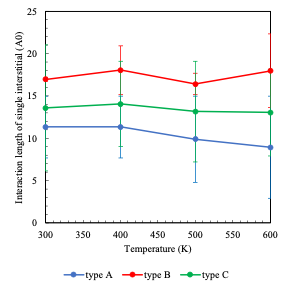
\includegraphics[width = 2.5in]{simple_IL_SI.png}}
\DIFdelbeginFL %DIFDELCMD < \subfloat[]{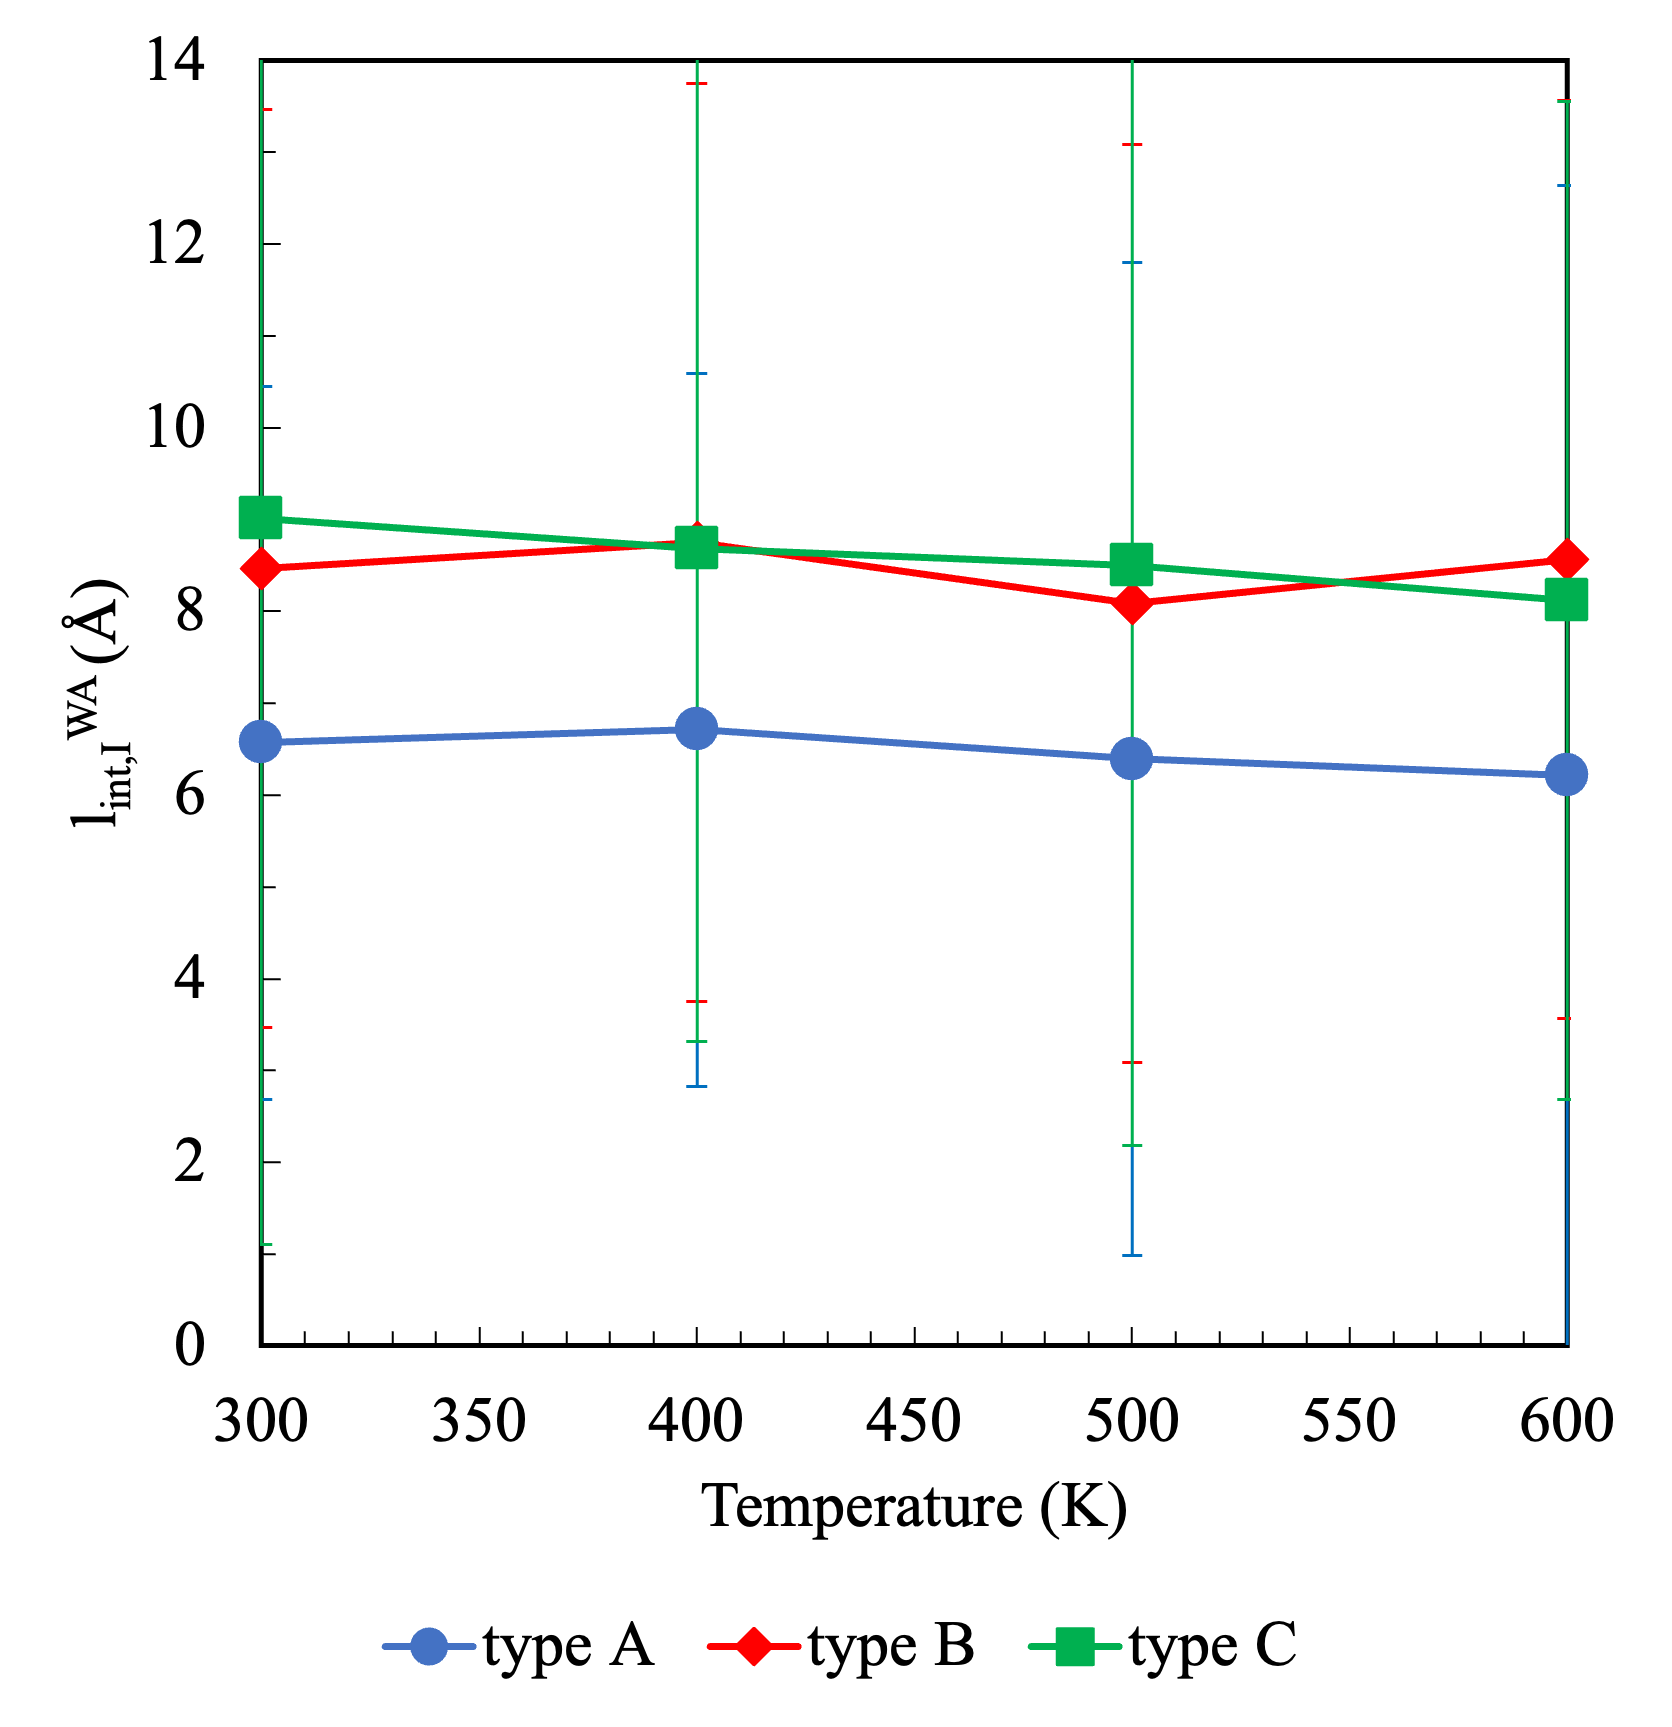
\includegraphics[width = 2.5in]{weighted_IL_SI.png}}
%DIFDELCMD < %%%
%DIF < \subfloat[]{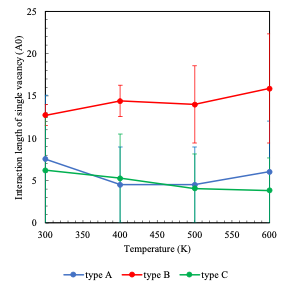
\includegraphics[width = 2.5in]{simple_IL_SV.png}} 
%DIFDELCMD < \subfloat[]{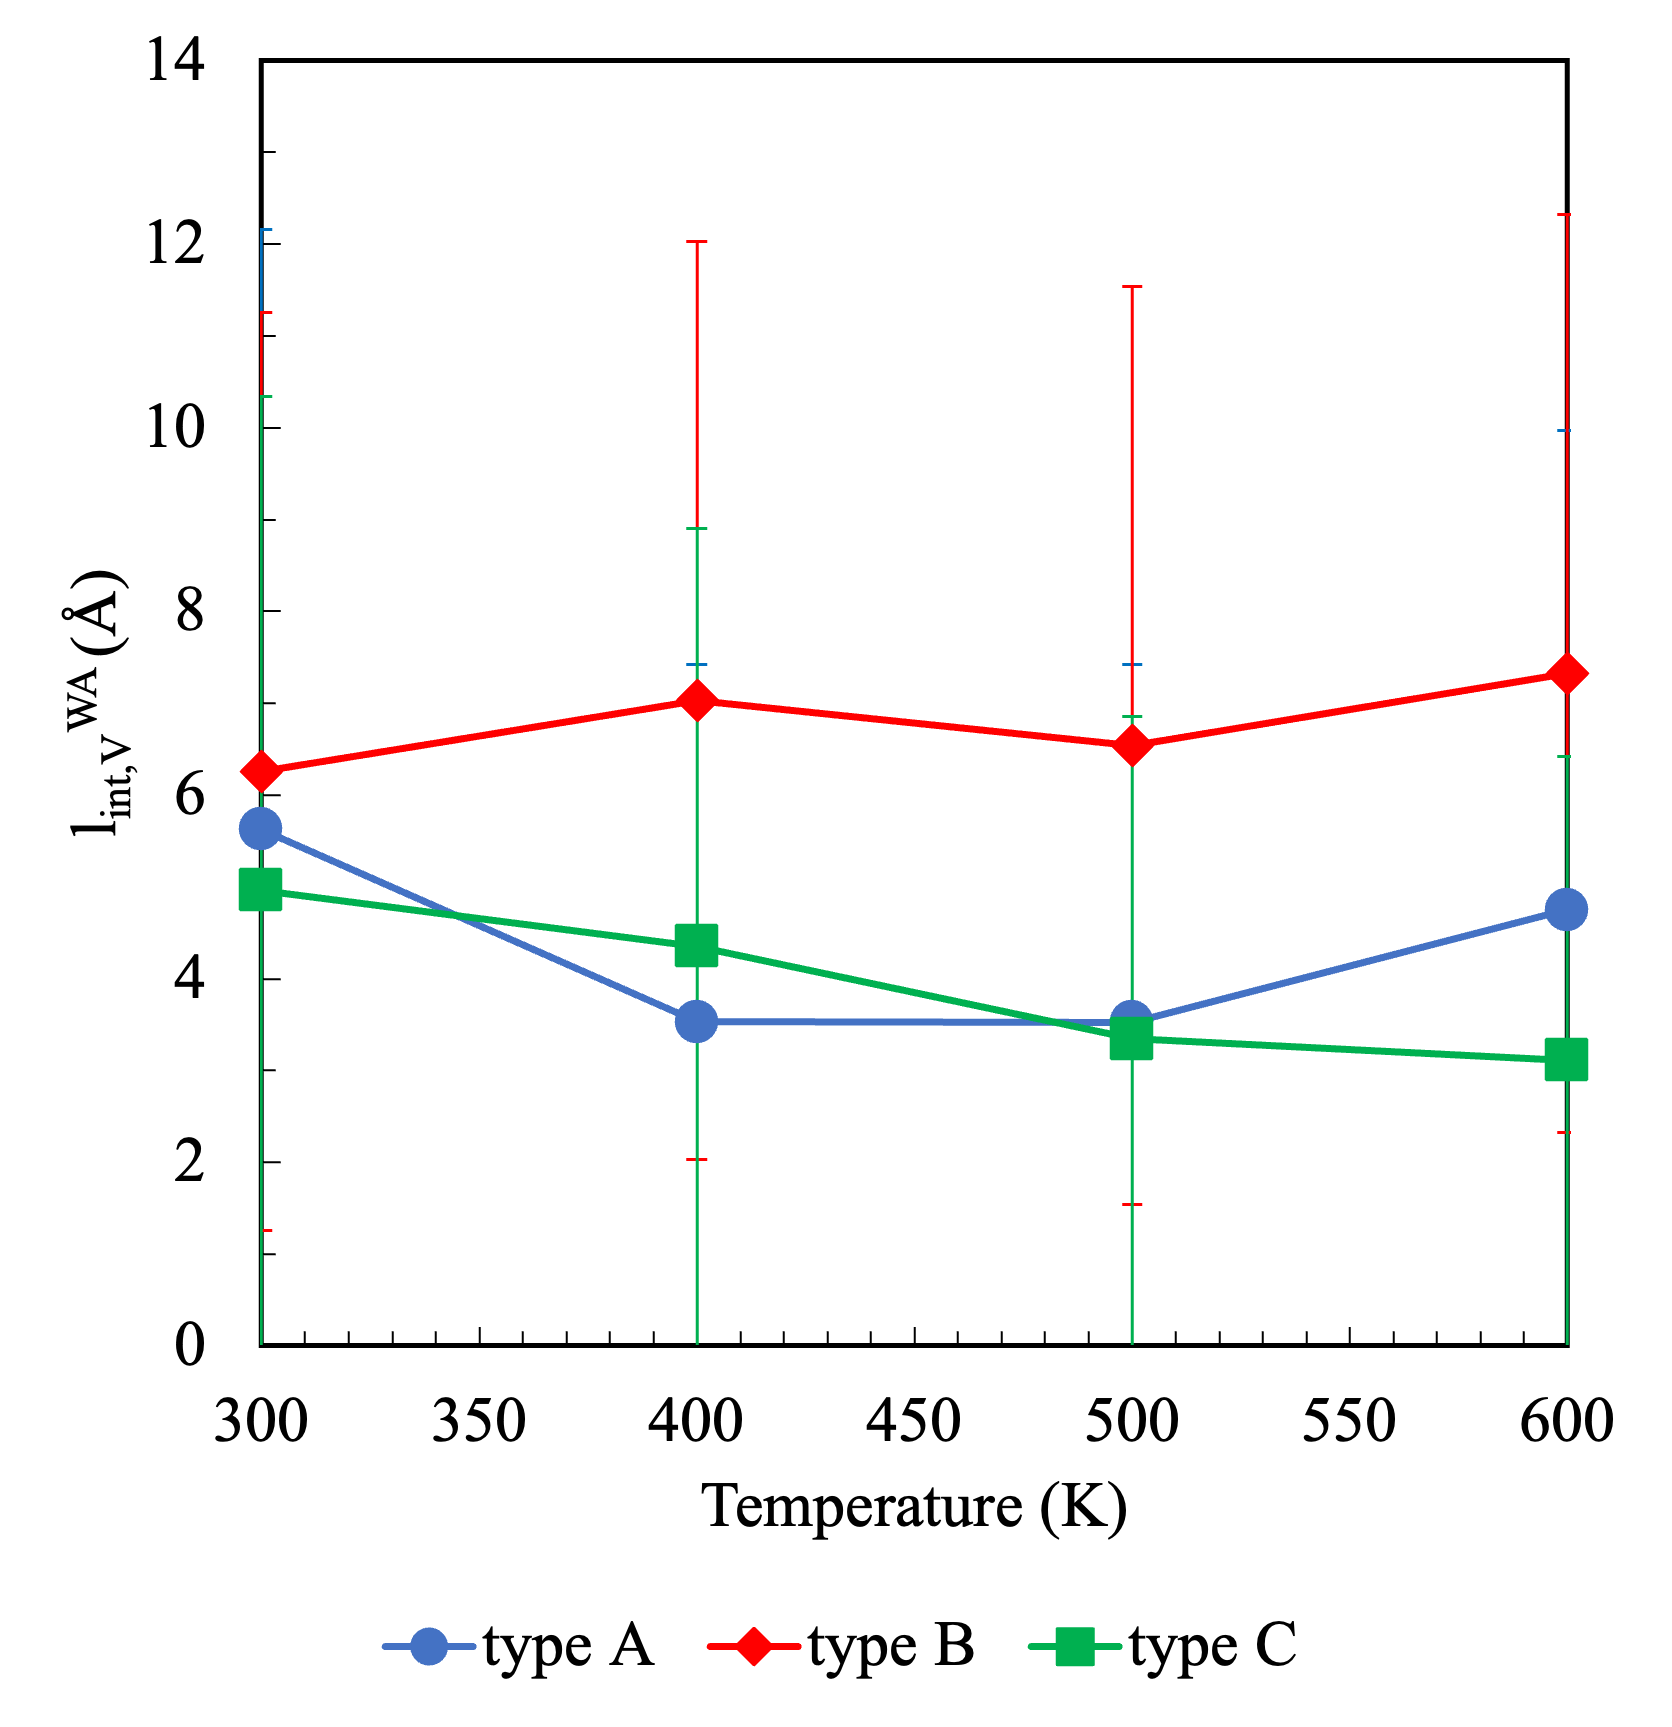
\includegraphics[width = 2.5in]{weighted_IL_SV.png}}
%DIFDELCMD < %%%
\DIFdelendFL \DIFaddbeginFL \subfloat[]{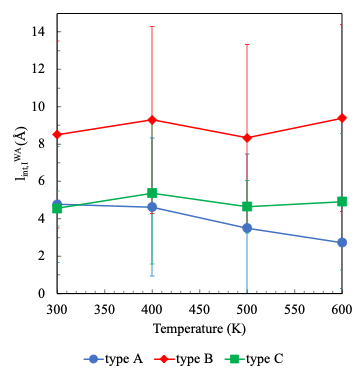
\includegraphics[width = 2.5in]{7_weighted_IL_SI.png}}
\subfloat[]{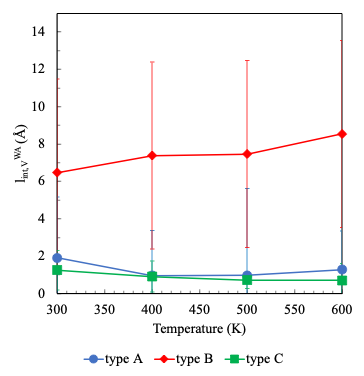
\includegraphics[width = 2.5in]{7_weighted_IL_SV.png}}
\DIFaddendFL \caption{Weighted average $l_{\mathrm{int}}$ of GBs in $\alpha$-U with (a) interstitial and (b) vacancy plotted over the temperature.}
\label{fig:IL}
\end{figure}

\FloatBarrier

\subsection{Diffusion along Grain Boundaries}
Diffusion requires both energy (from lattice vibrations) and a pathway to the target site. Transport of point defects along GBs is a point of interest for radiation damage analysis and stress relaxation. In this section, the self-diffusion of $\alpha$-U atoms along the six studied GBs is reported. It should be noted that self-diffusion of $\alpha$-U along low-energy GBs is not observed within the studied temperature range without the introduction of a point defect. This is due to the relatively \textit{clean} structure of the GB, where lattice positions are maintained. After introducing an additional point defect within the GB interaction zone of the respective GBs, self-diffusion along GBs is observed. Thus, in the following discussions the A1, B1, and C1 GBs each only have two data sets of diffusion (one with a vacancy and another with an interstitial). This is not required for high-energy GBs where the local structure displays sufficient atomic distortion/displacement to allow for inherent diffusion without the addition of a point defect. Thus, the A2, B2, and C2 GBs each have three data sets (only GB, with a vacancy, and with an interstitial). In the following sections, GB self-diffusion in the presence of a vacancy and an interstitial is represented by GB+V and GB+I, respectively. 


\subsubsection{Low-Energy Grain Boundaries}

\par The diffusivity along low-energy GBs is shown in \Cref{fig:Dif_fit1} with an accompanying Arrhenius fit. Included error bars represent one standard error of the mean. The three low-energy GBs exhibit higher self-diffusivity in the presence of an interstitial compared to an added vacancy. The self-diffusion of GB+V and GB+I of A1 and B1 GBs tend to converge as the temperature increases\DIFdelbegin \DIFdel{, while }\DIFdelend \DIFaddbegin \DIFadd{. On the other hand, }\DIFaddend self-diffusivity for the lowest formation energy GB considered in the current work, C1, maintains an approximately constant ratio (2.2 to 2.5) between \DIFdelbegin \DIFdel{the two defect cases}\DIFdelend \DIFaddbegin \DIFadd{GB+V and GB+I condition}\DIFaddend . One reason for this might be the type of diffusion path. For GB+V diffusion of A1, B1, and C1 GBs, two-dimensional diffusion was observed. This means that diffusion occurs all along the grain boundary plane. A similar diffusion pathway is followed for the GB+I of A1 and B1 GBs, but not the C1 GB. In contrast, the C1 GB demonstrates a ring diffusion mechanism for an interstitial where the rings are aligned parallel to the $\langle$0 0 1$\rangle$ tilt axis and on the (100) shear plane. These rings may hinder faster GB+I diffusion at lower temperatures. For the GB+V case, the A1 GB shows the lowest diffusivity, while the B1 has the highest diffusivity below 600 K and C1 has the highest above 600 K. For the GB+I case, B1 always possesses a higher diffusivity than the other low-energy GBs. 

\begin{figure}[h!]
\centering
\DIFdelbeginFL %DIFDELCMD < \subfloat[]{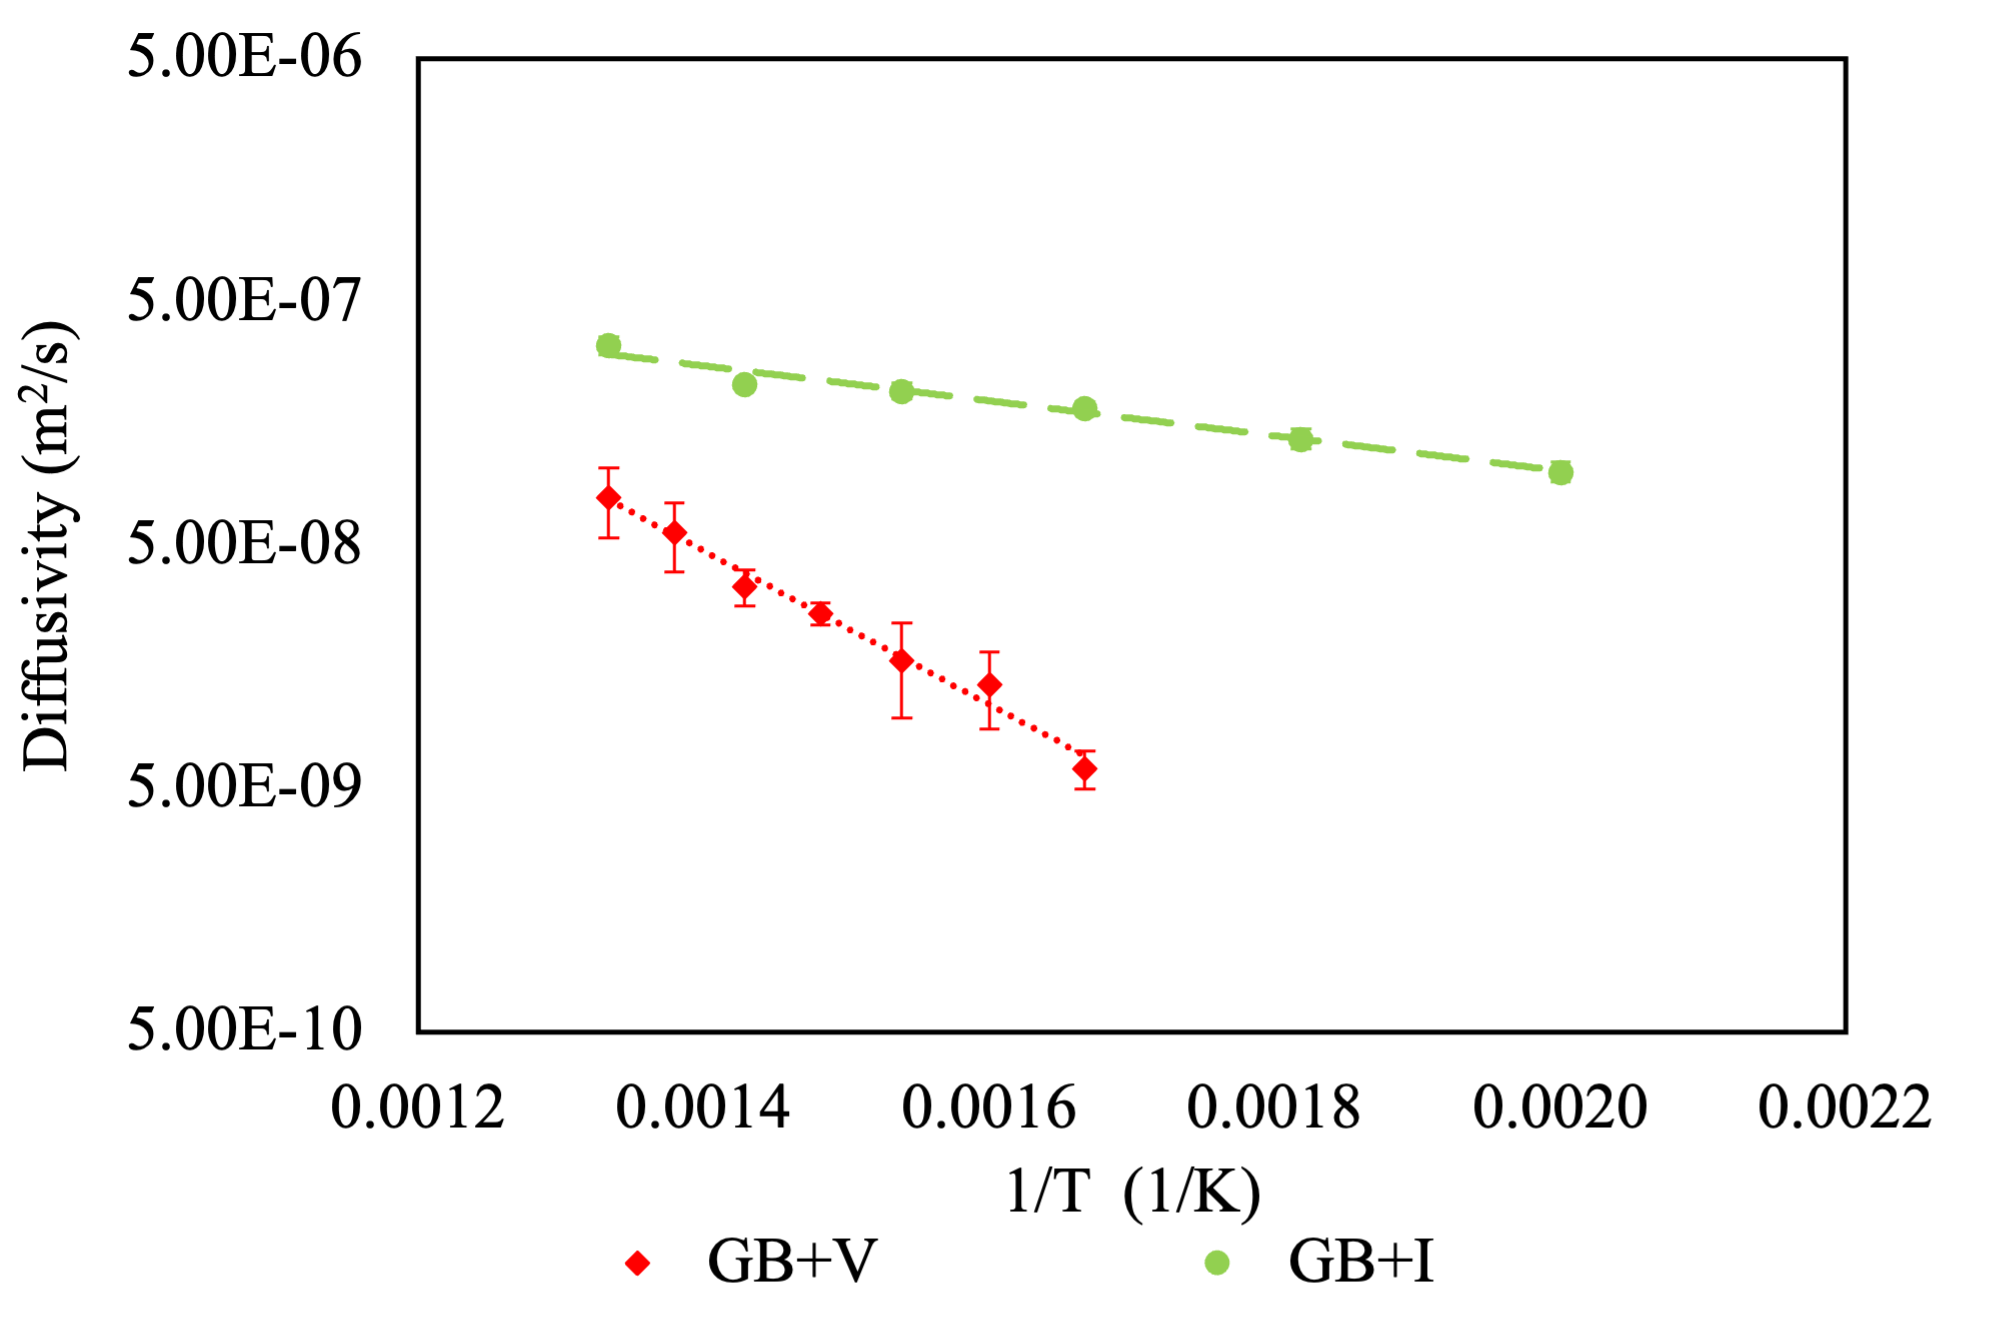
\includegraphics[width = 2.25in]{A1_diffusion.png}}
%DIFDELCMD < \subfloat[]{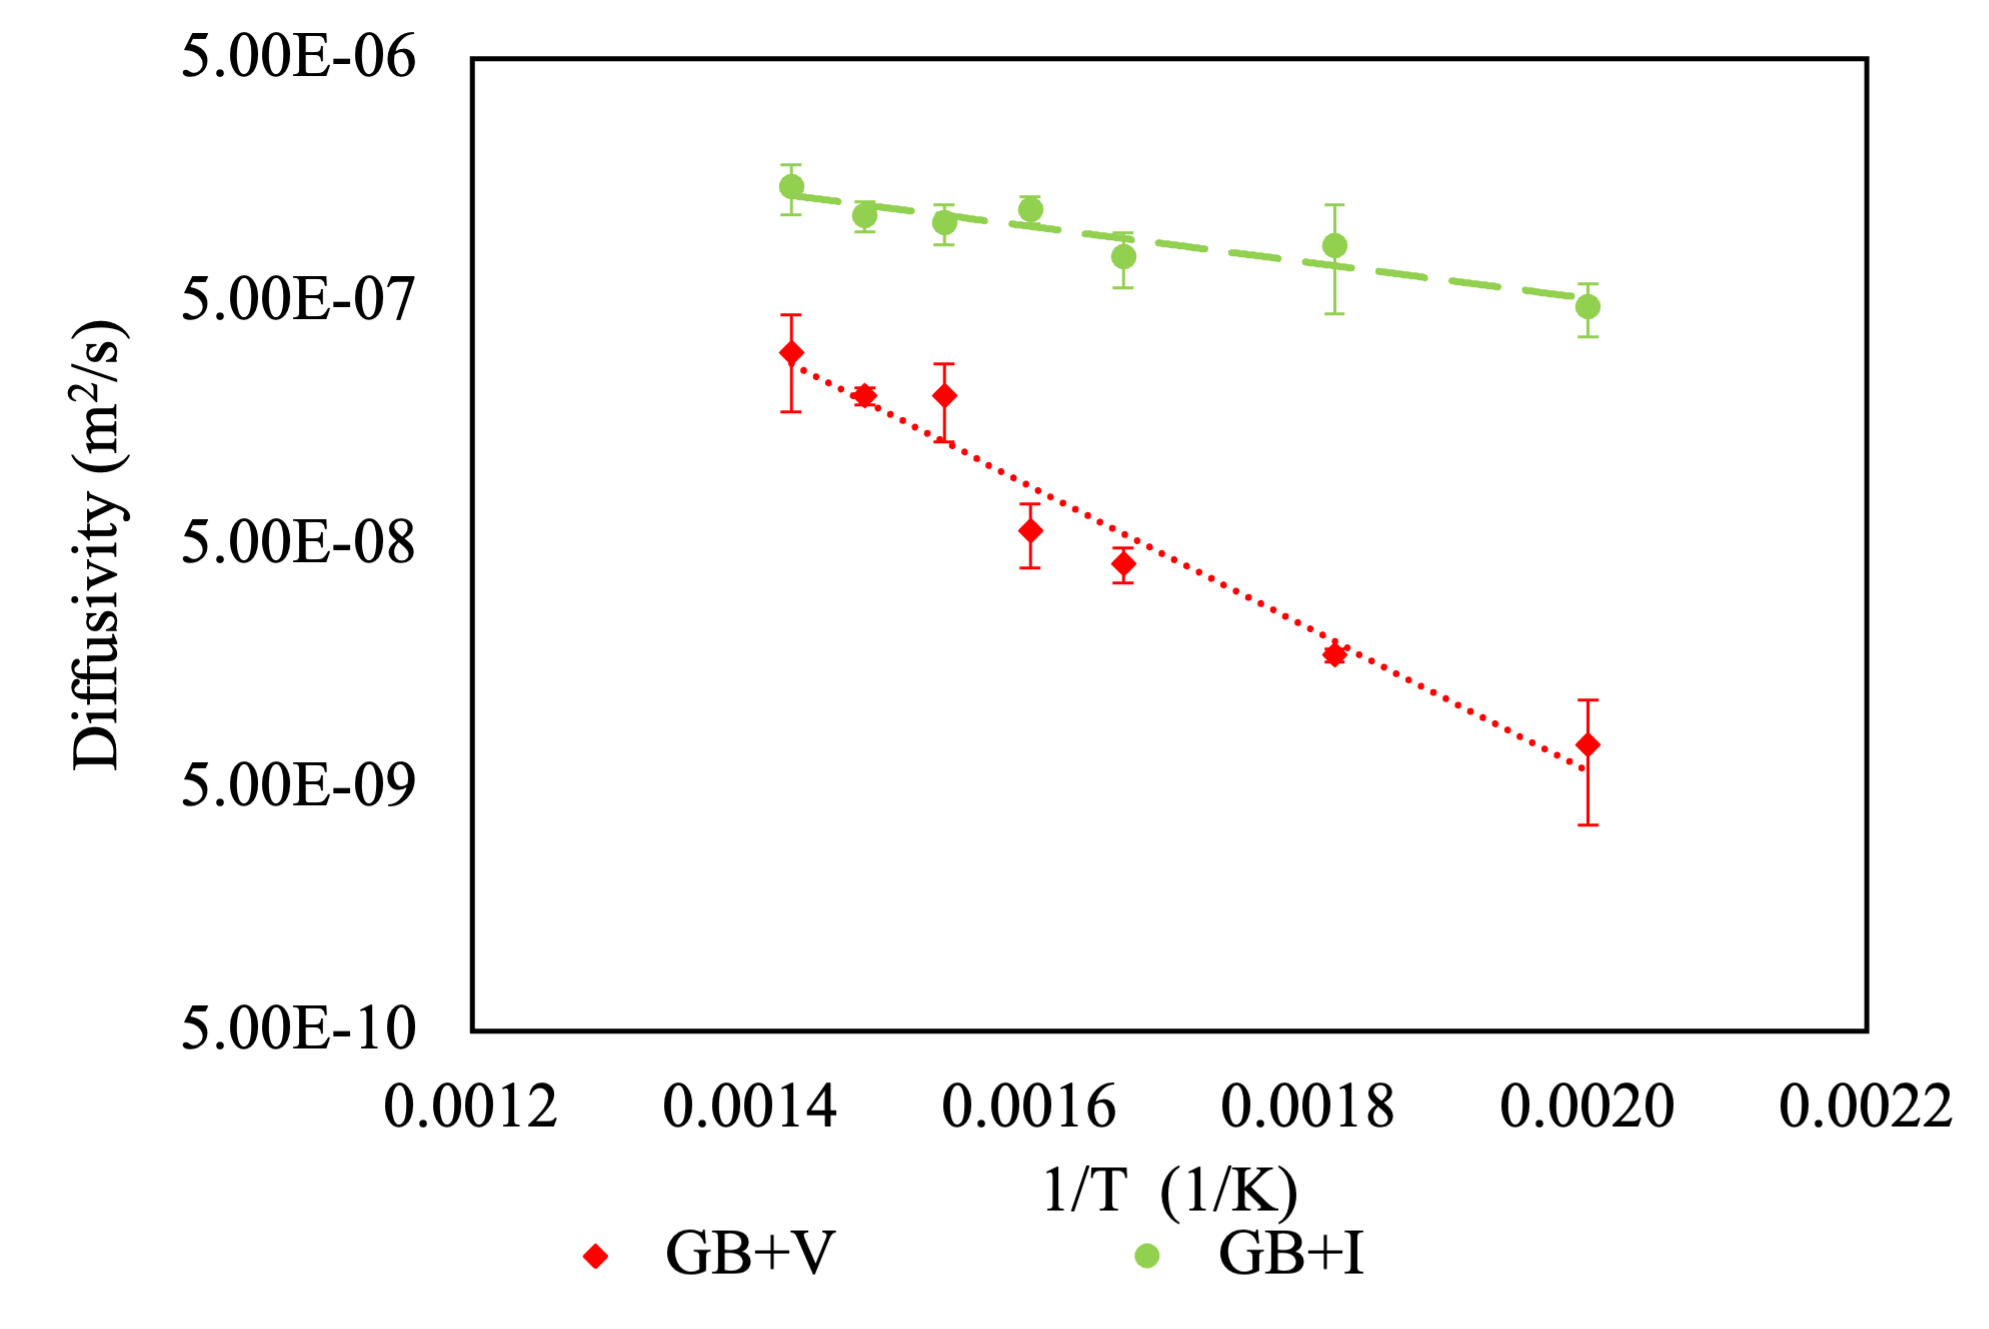
\includegraphics[width = 2.25in]{B1_diffusion.png}} 
%DIFDELCMD < \subfloat[]{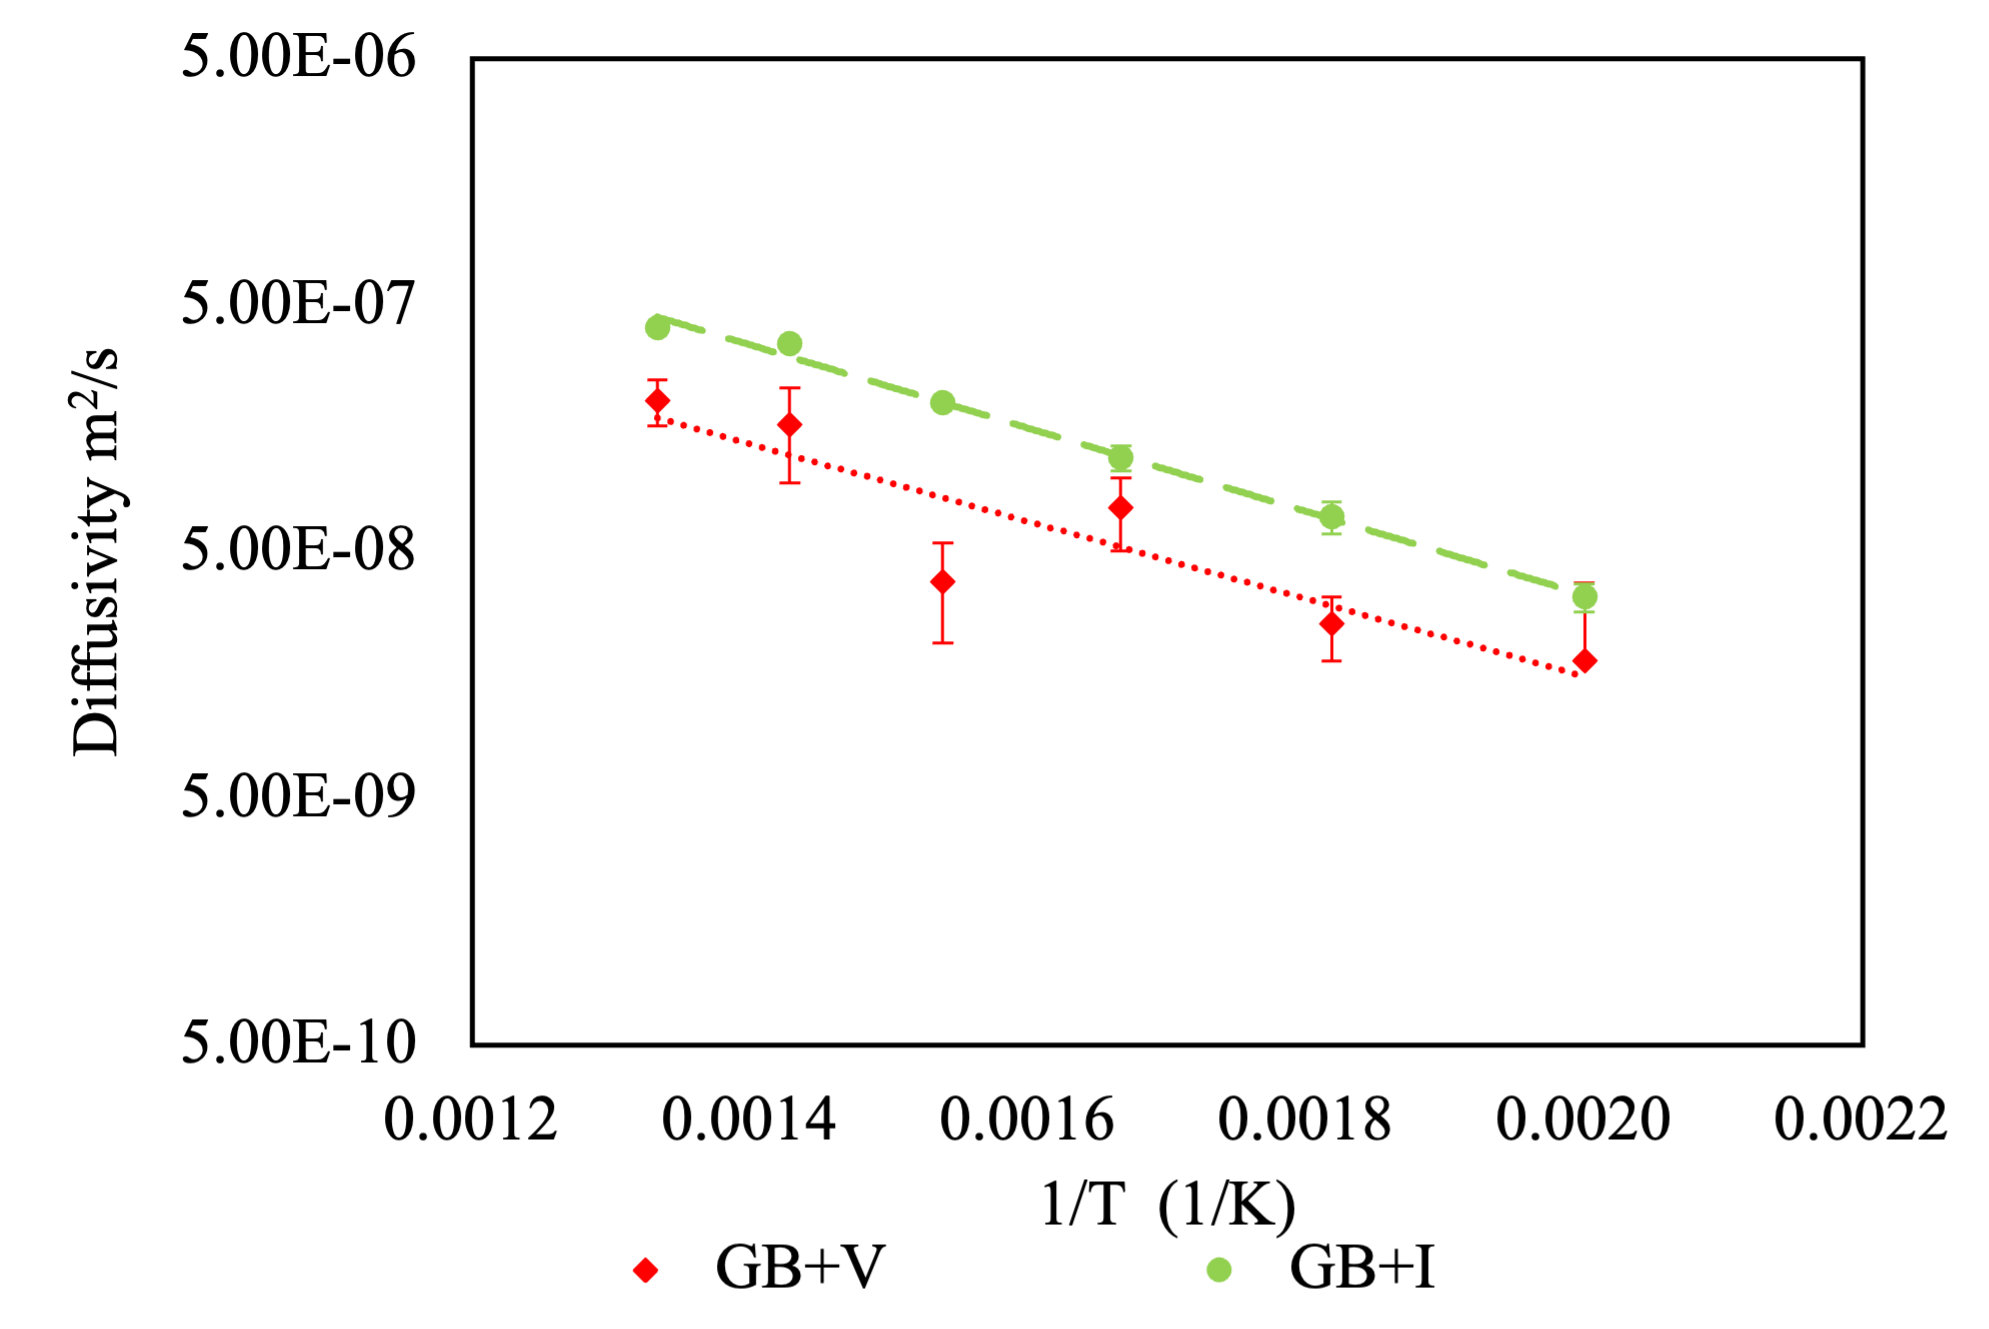
\includegraphics[width = 2.25in]{C1_diffusion.png}}%%%
\DIFdelendFL \DIFaddbeginFL \subfloat[]{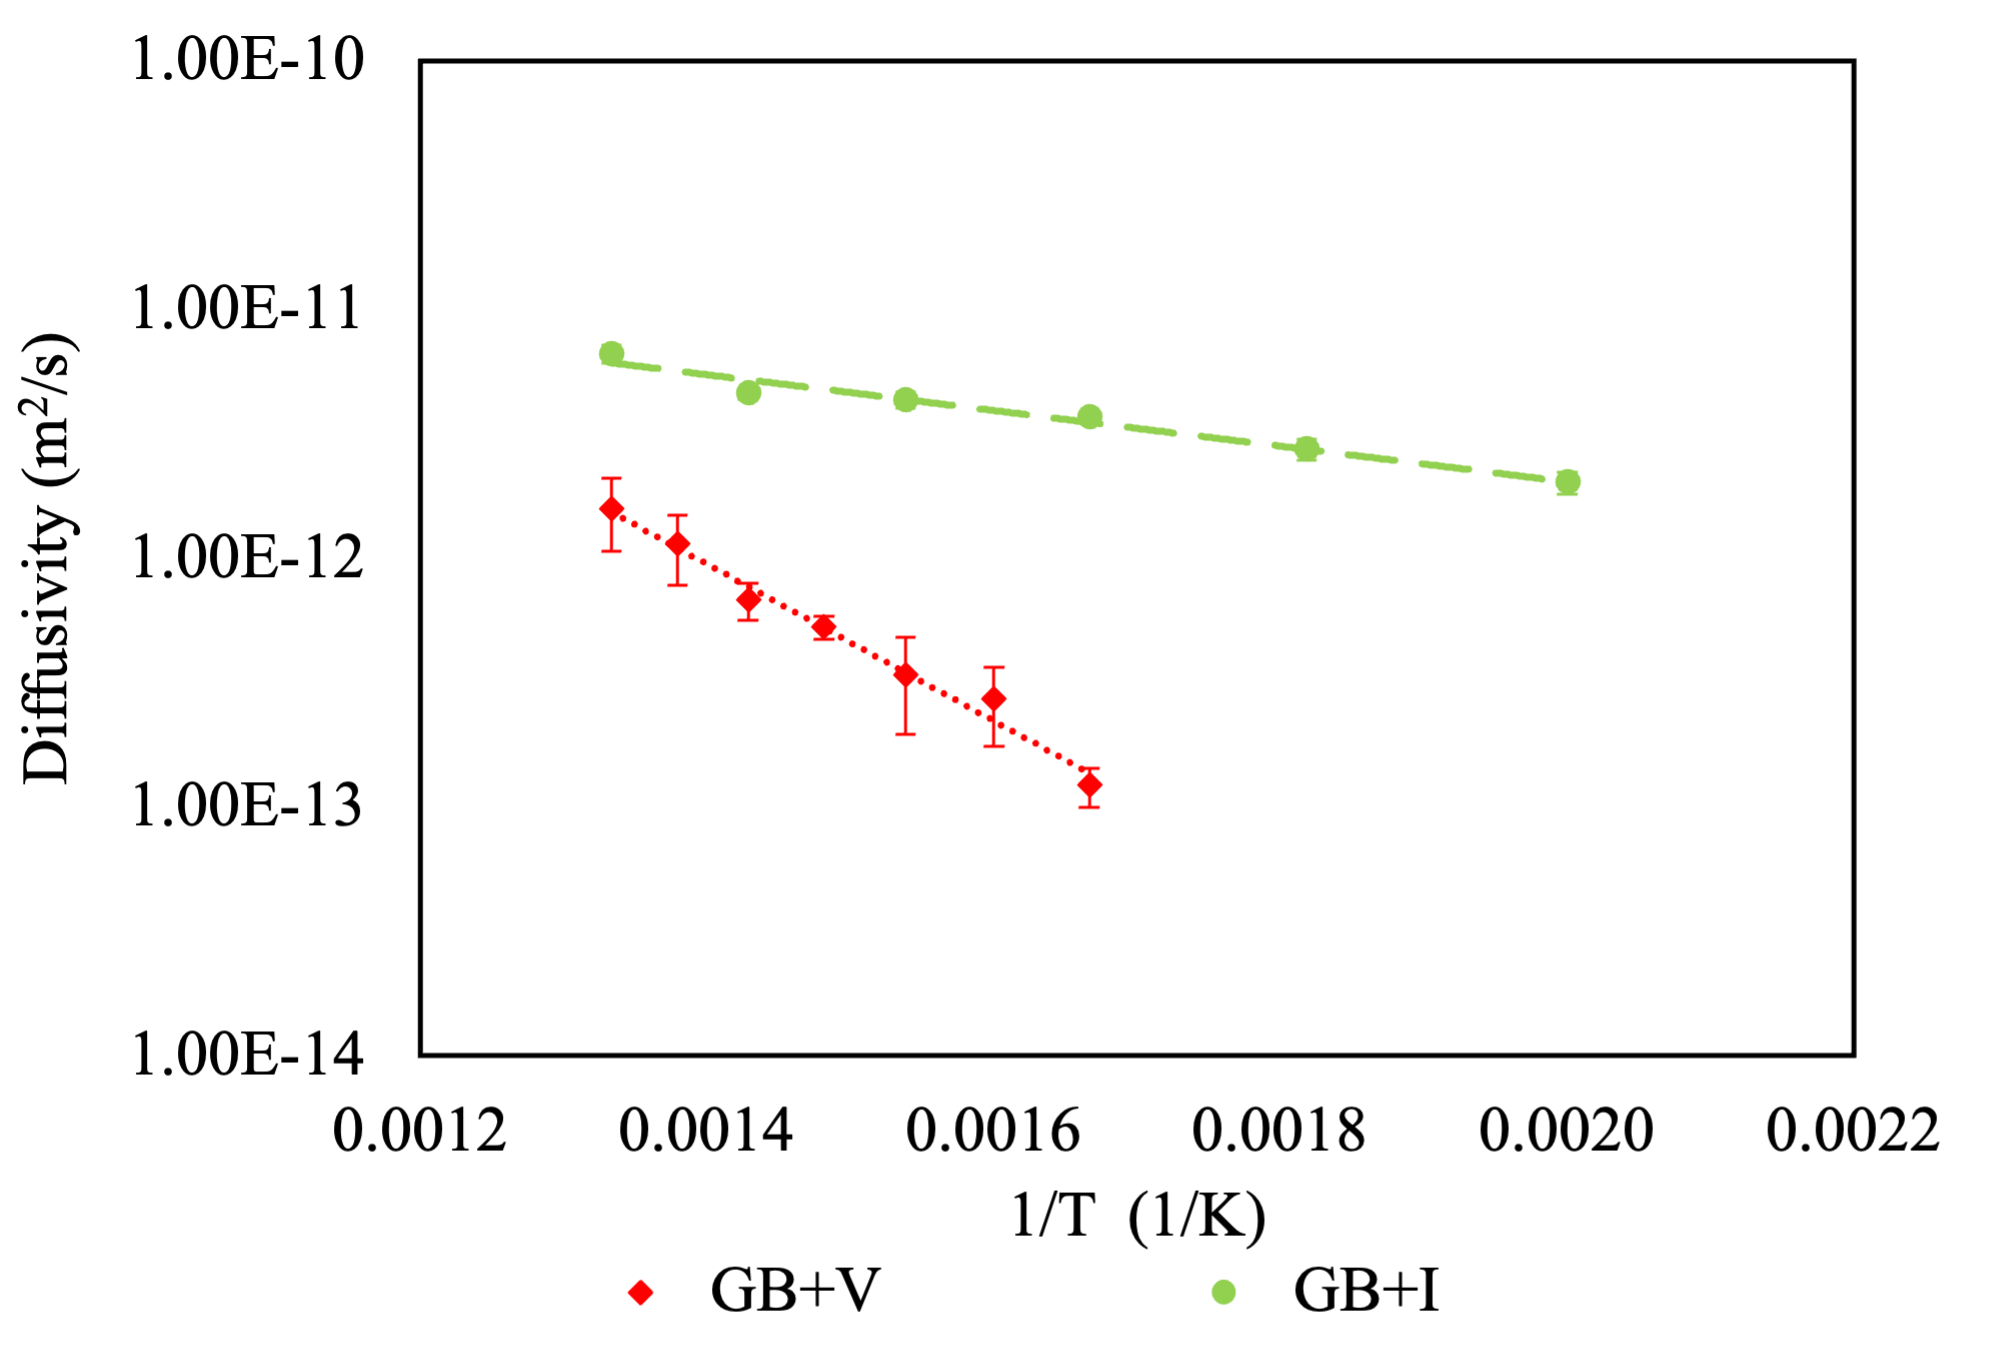
\includegraphics[width = 2.25in]{8_A1_diffusion.png}}
\subfloat[]{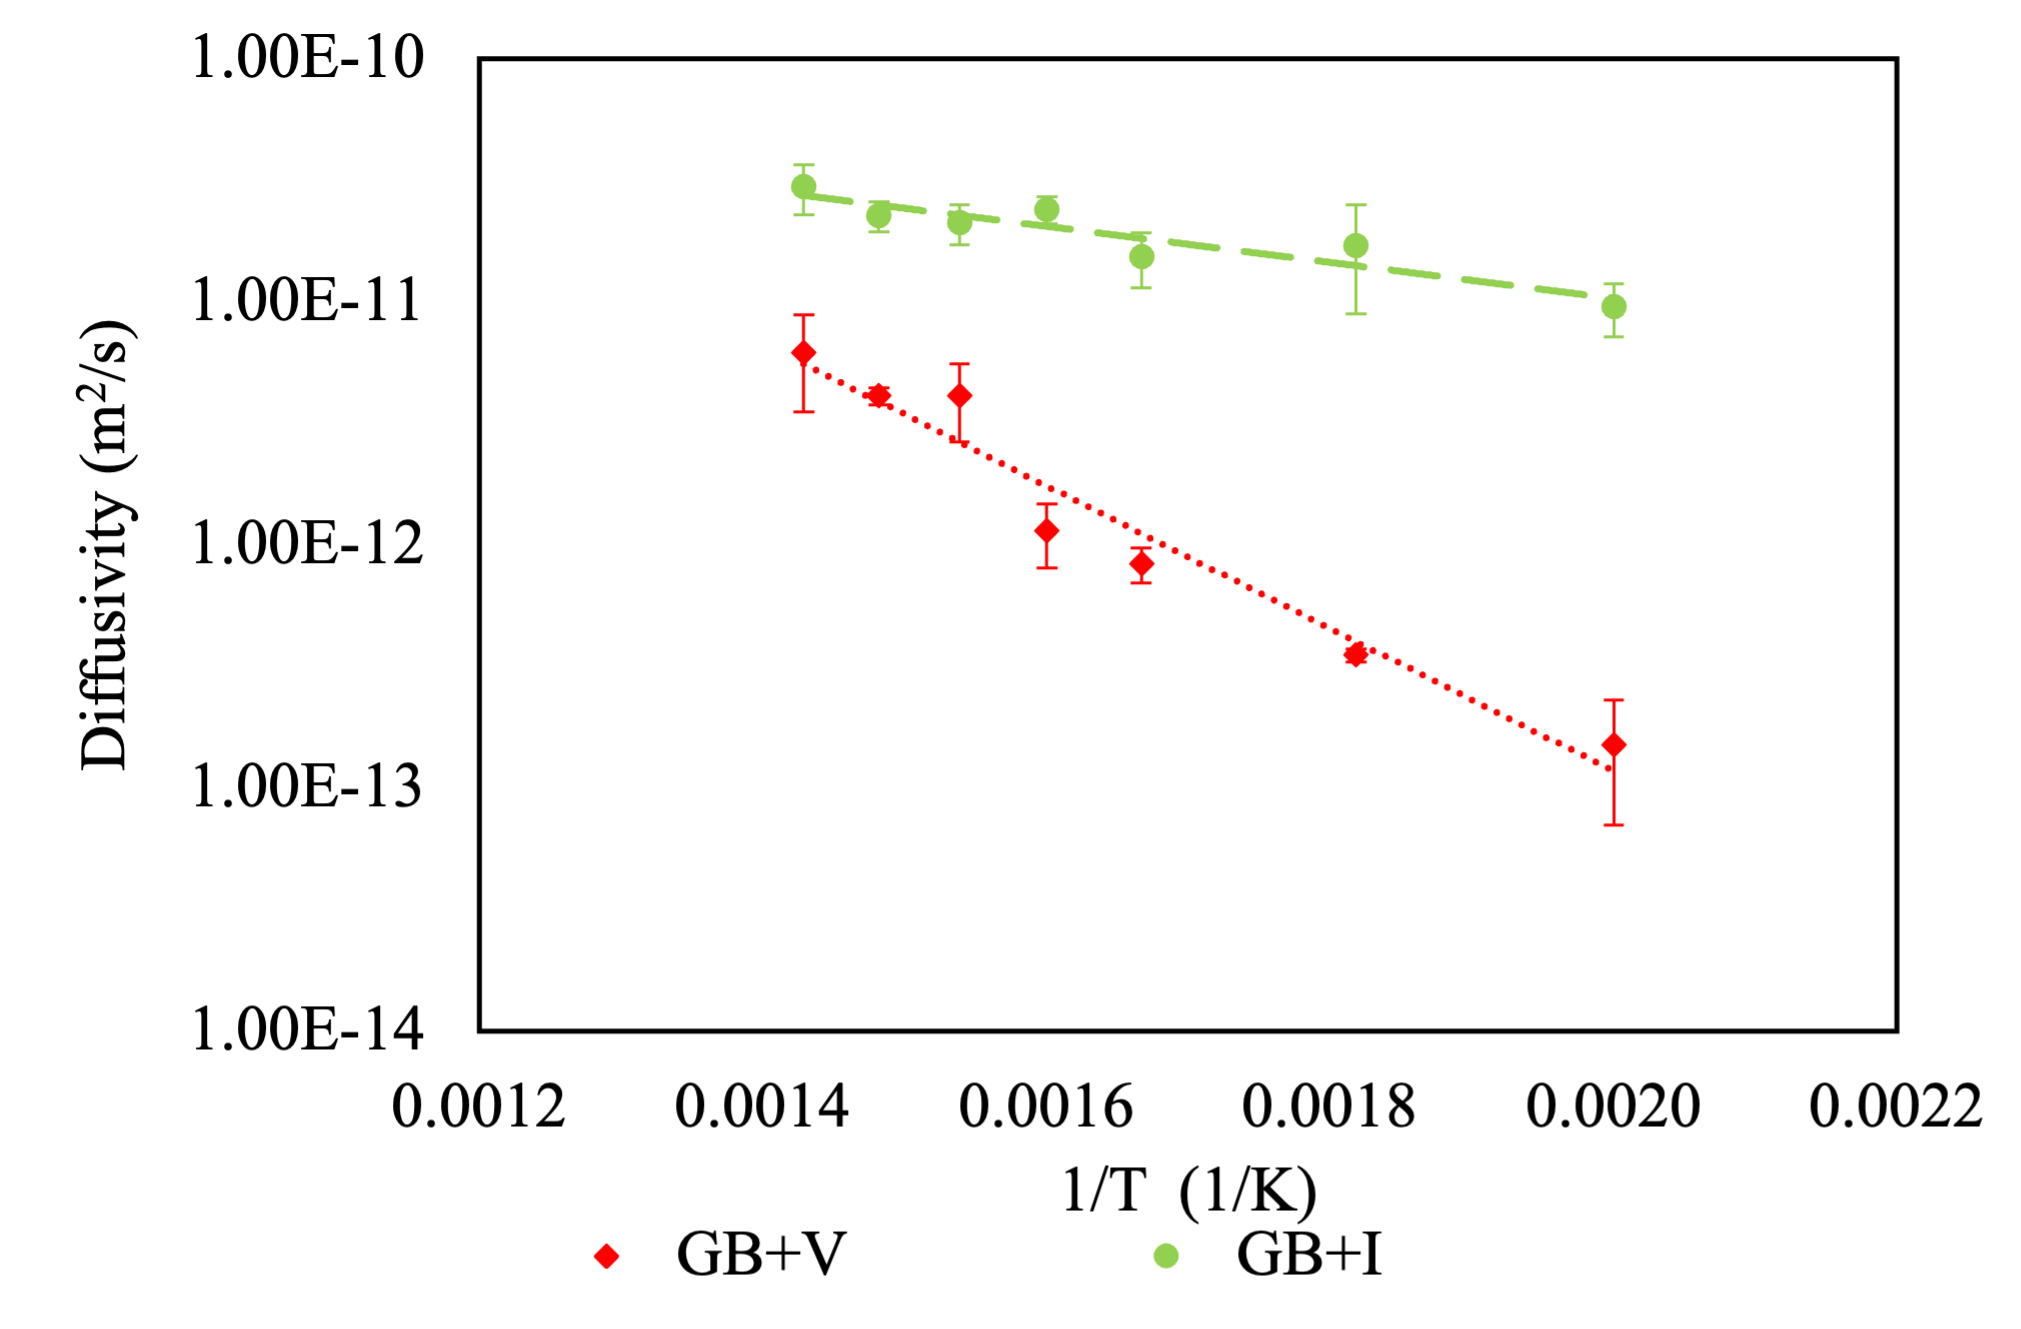
\includegraphics[width = 2.25in]{8_B1_diffusion.png}} 
\subfloat[]{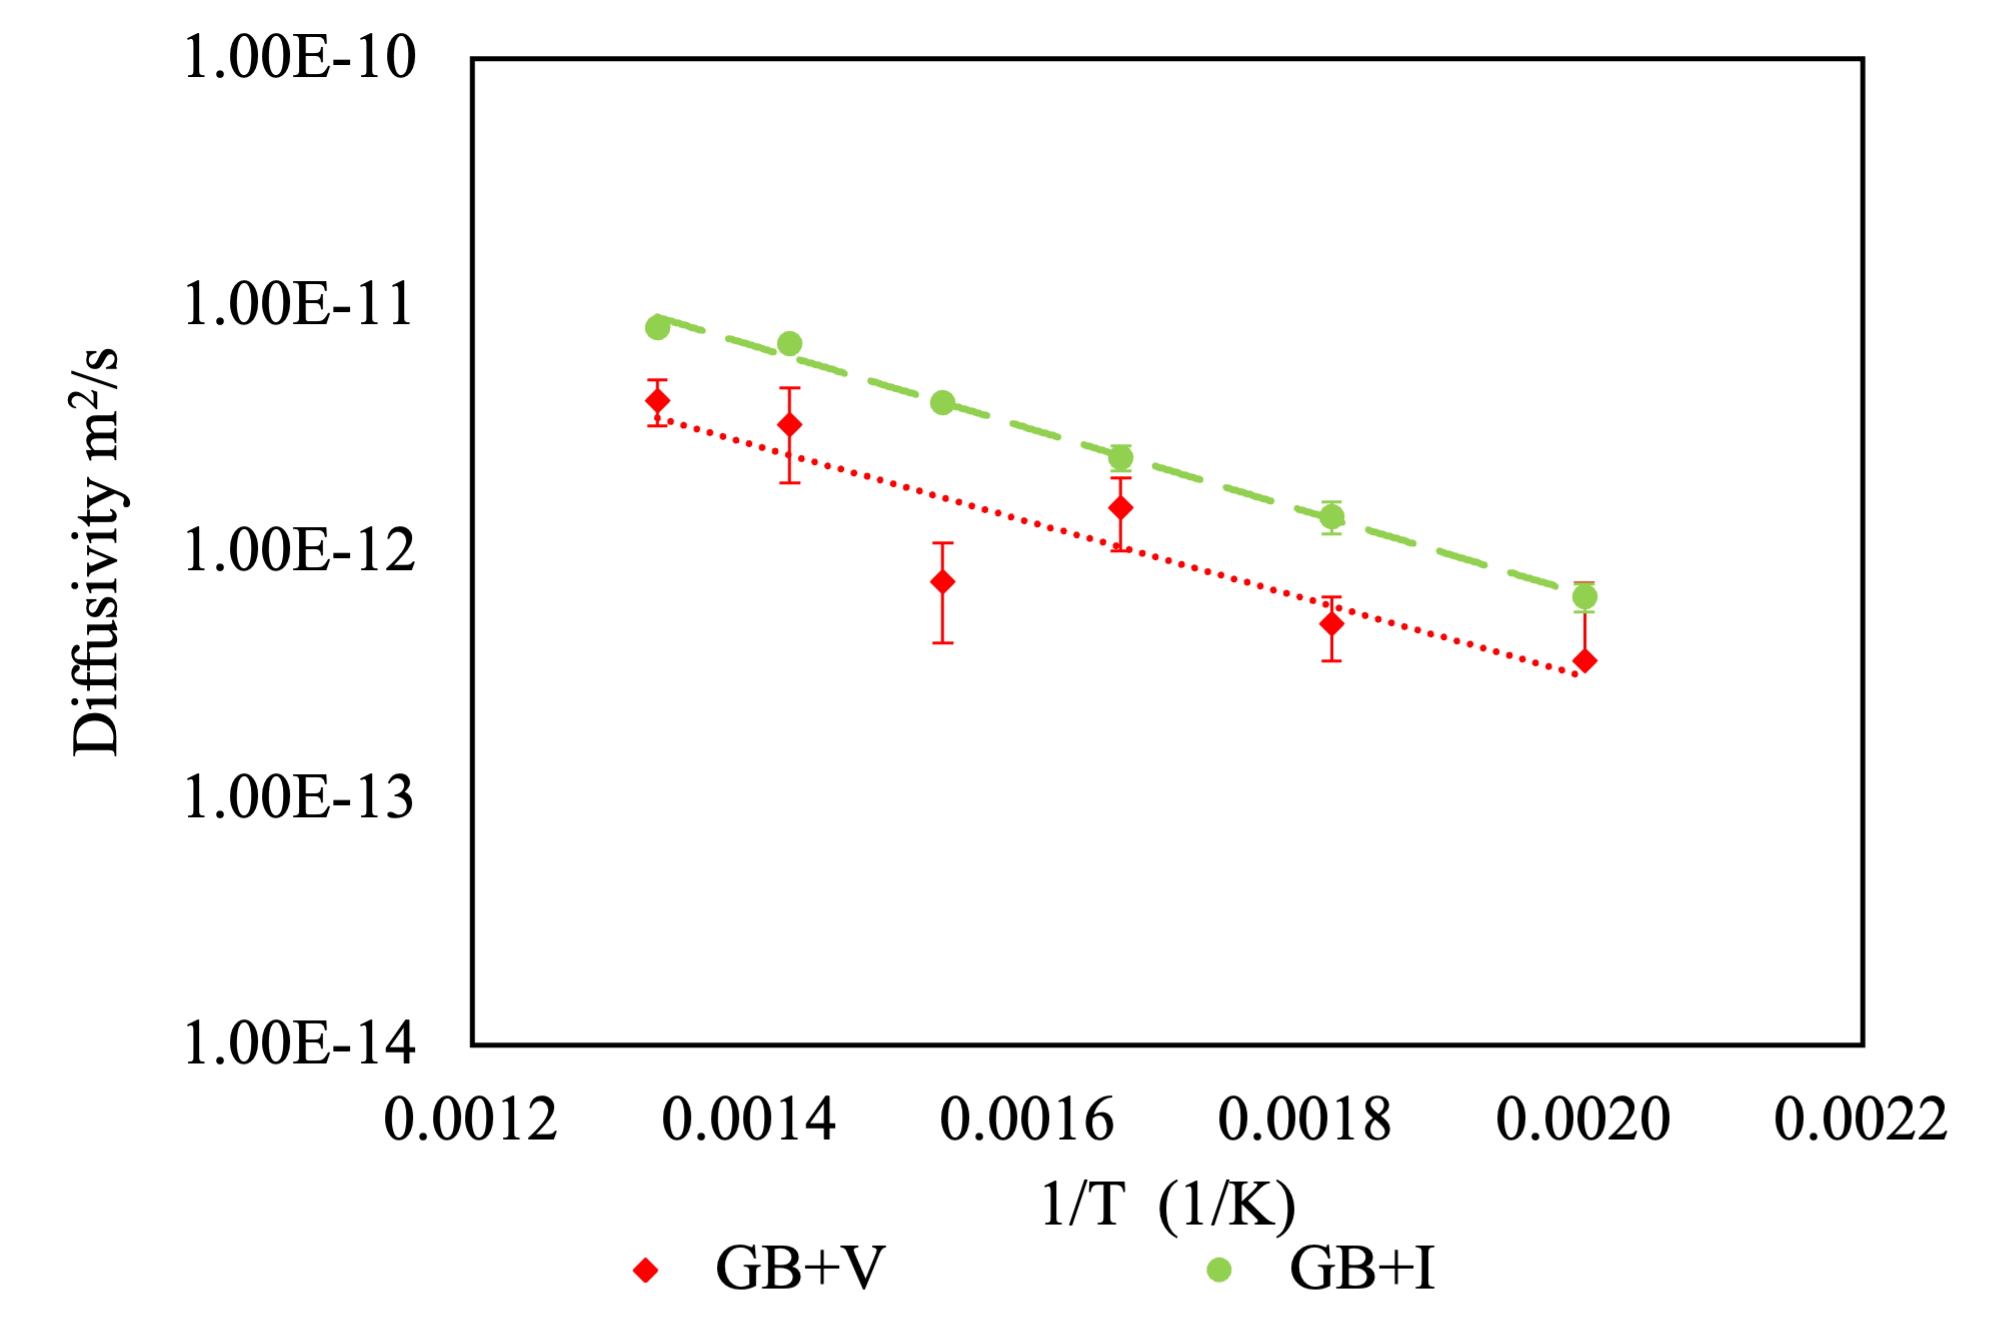
\includegraphics[width = 2.25in]{8_C1_diffusion.png}}\DIFaddendFL \\
\caption{Arrhenius plots of $\alpha$-U diffusion through (a) A1, (b) B1, and (c) C1 grain boundaries. GB+V means diffusion with an added vacancy and GB+I means diffusion with an added interstitial. Straight lines here represent the fitted Arrhenius equation and the error bars represent one standard error. Fitted values are tabulated in the Appendix (\ref{tab:migra} and \ref{tab:pre}).}
\label{fig:Dif_fit1}
\end{figure}

\subsubsection{High-Energy Grain Boundaries}

\par The diffusion coefficients for the high-energy GBs are shown in \Cref{fig:Dif_fit2}. Diffusion in the high-energy grain boundaries displays a unique behavior compared to that of the low-energy grain boundaries. Pipe diffusion (1-D diffusion) is observed in the A2 and C2 GBs, where the pipes are oriented normal to the shear plane. Thus, for the A2 GB, the pipe axis is parallel to the [001] direction and for the C2 GB it is parallel to the [100] direction. Pipe diffusion is not observed for the B2 GB, which has the shear plane normal to the [010] direction. From experimental studies, the self-diffusion of $\alpha$-U atoms in the [100] and [001] directions is about 20 times higher than that of the [010] direction at 900 K \cite{aniso_self_diff}. One of the reasons for the slow diffusivity in the [010] direction is the stacking of the corrugated planes in the [010] direction. Thus, it appears that some of the anisotropic characteristics of the bulk self-diffusion in $\alpha$-U may transfer to the study of grain boundary diffusion. A recent MD study \cite{WANG2023154289} on point defect diffusivity through bulk $\alpha$-U shows that for interstitials, [100] is the slowest diffusion direction, whereas for vacancies, it is [010] direction. As the high-energy GBs contain more disorder and thus void space, this pipe diffusion behavior might be occurring due to the presence of vacancies within the GB core.

\begin{figure}[h!]
\centering
\DIFdelbeginFL %DIFDELCMD < \subfloat[]{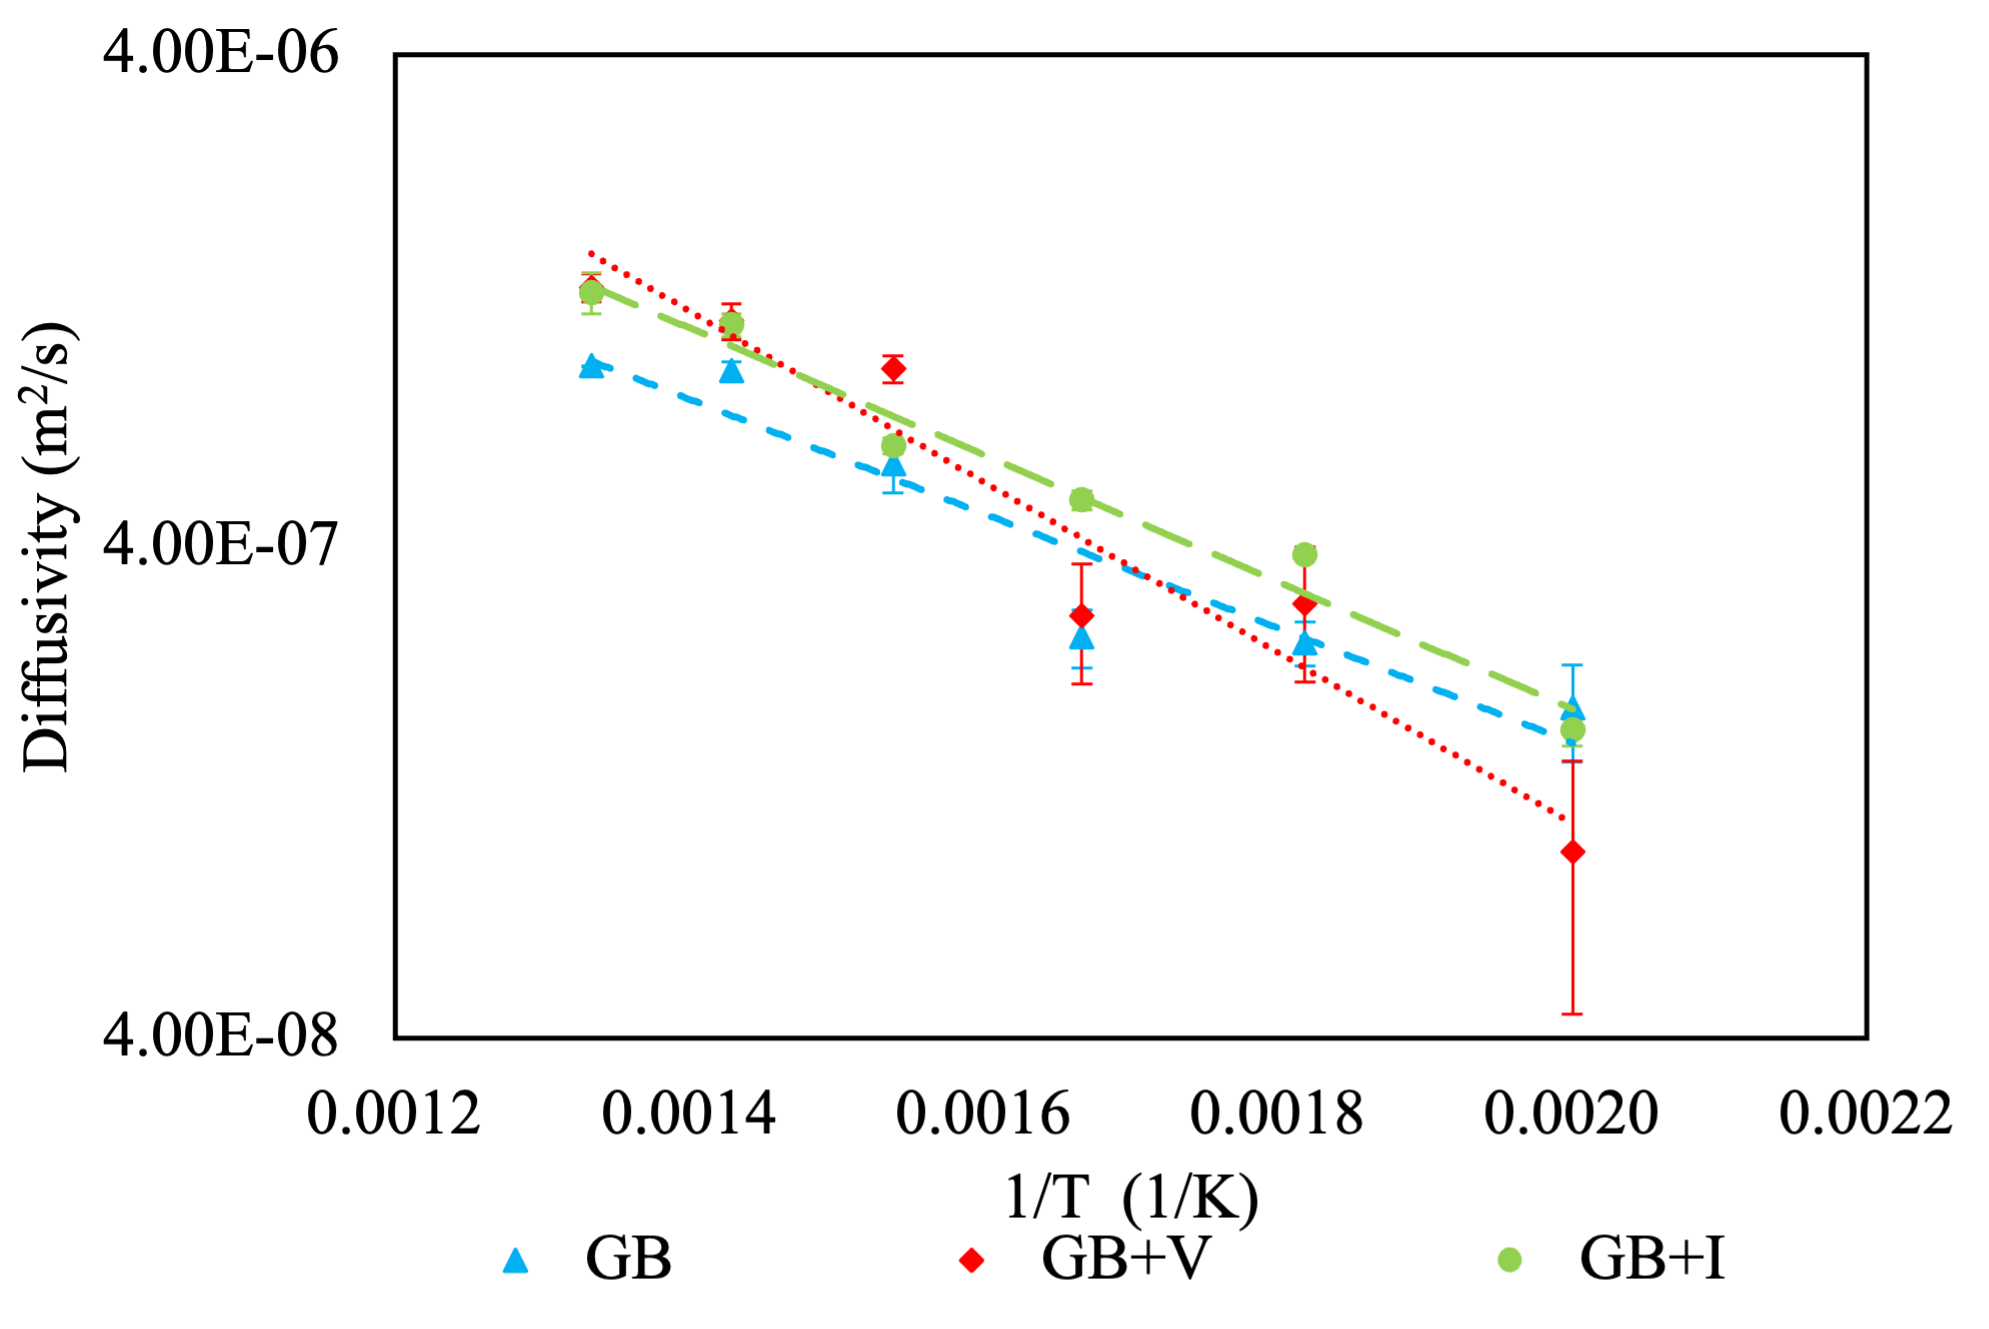
\includegraphics[width = 2.25in]{A2_diffusion.png}}
%DIFDELCMD < \subfloat[]{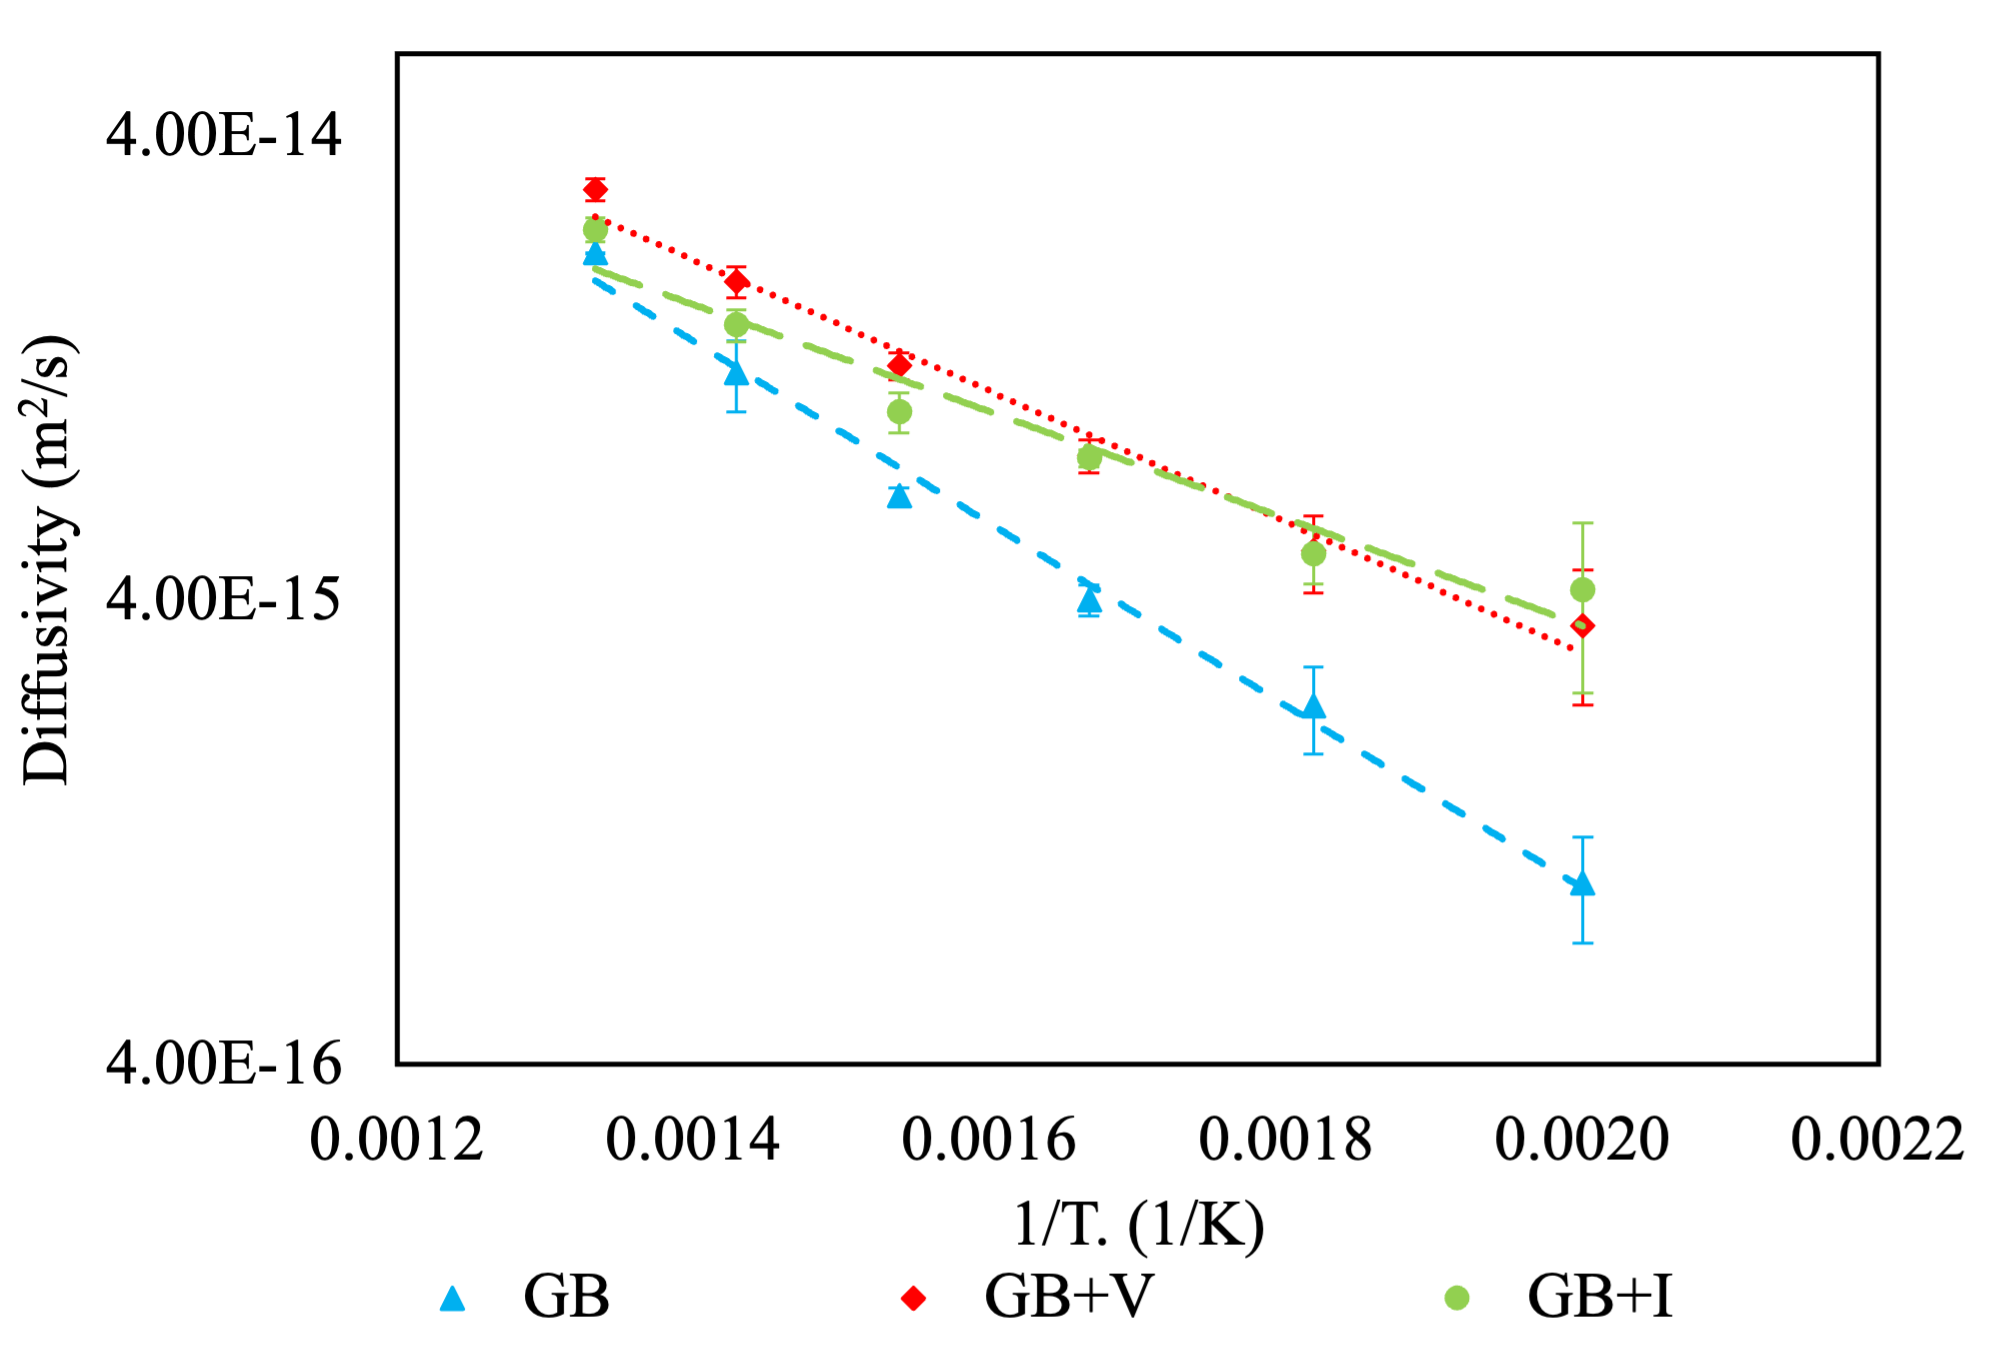
\includegraphics[width = 2.25in]{B2_diffusion.png}} 
%DIFDELCMD < \subfloat[]{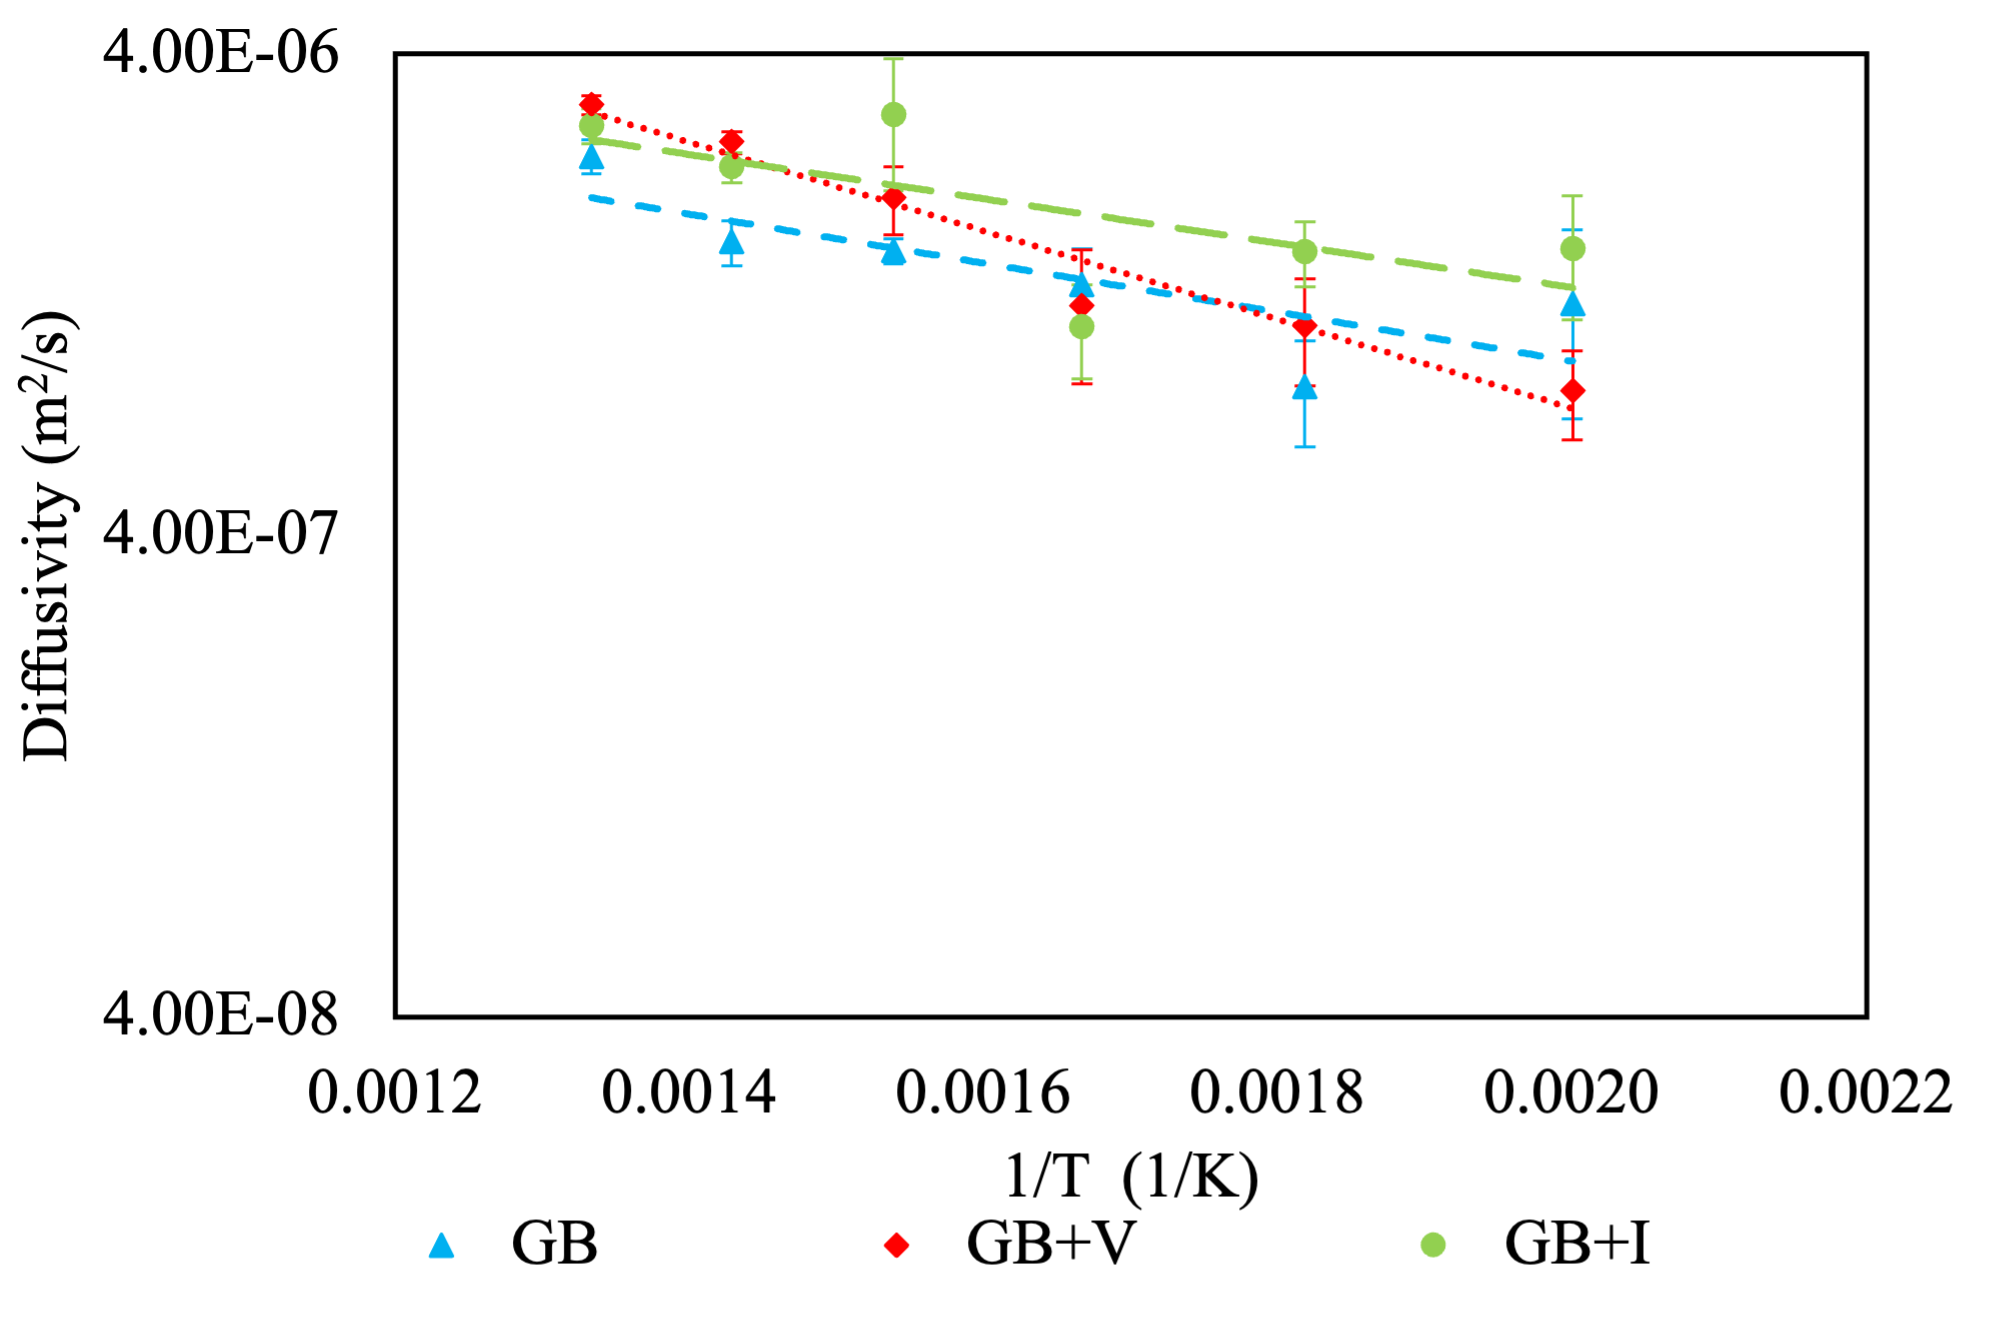
\includegraphics[width = 2.25in]{C2_diffusion.png}}%%%
\DIFdelendFL \DIFaddbeginFL \subfloat[]{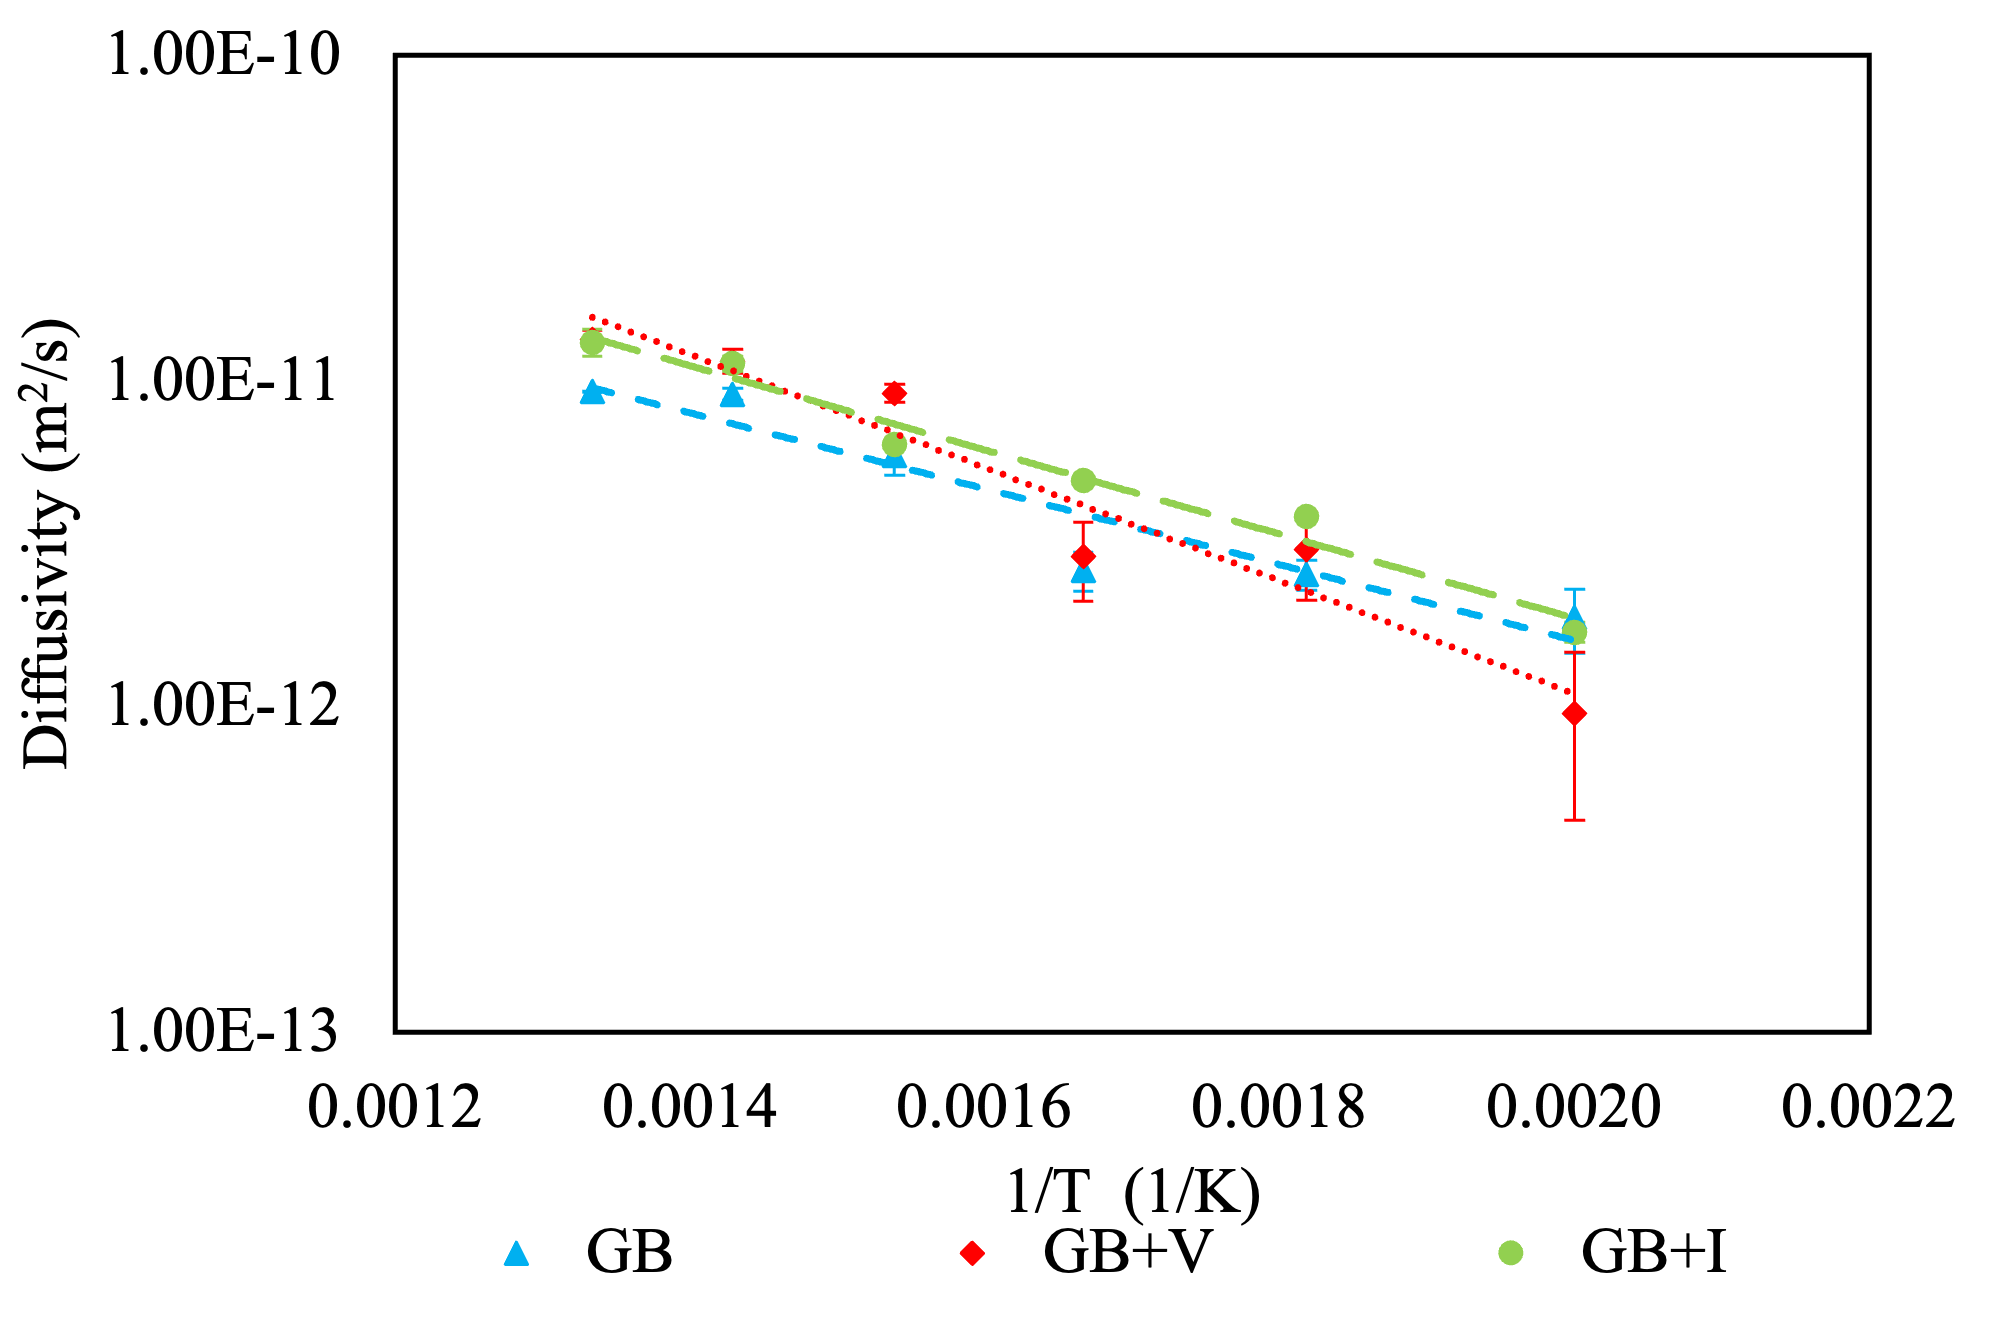
\includegraphics[width = 2.25in]{9_A2_diffusion.png}}
\subfloat[]{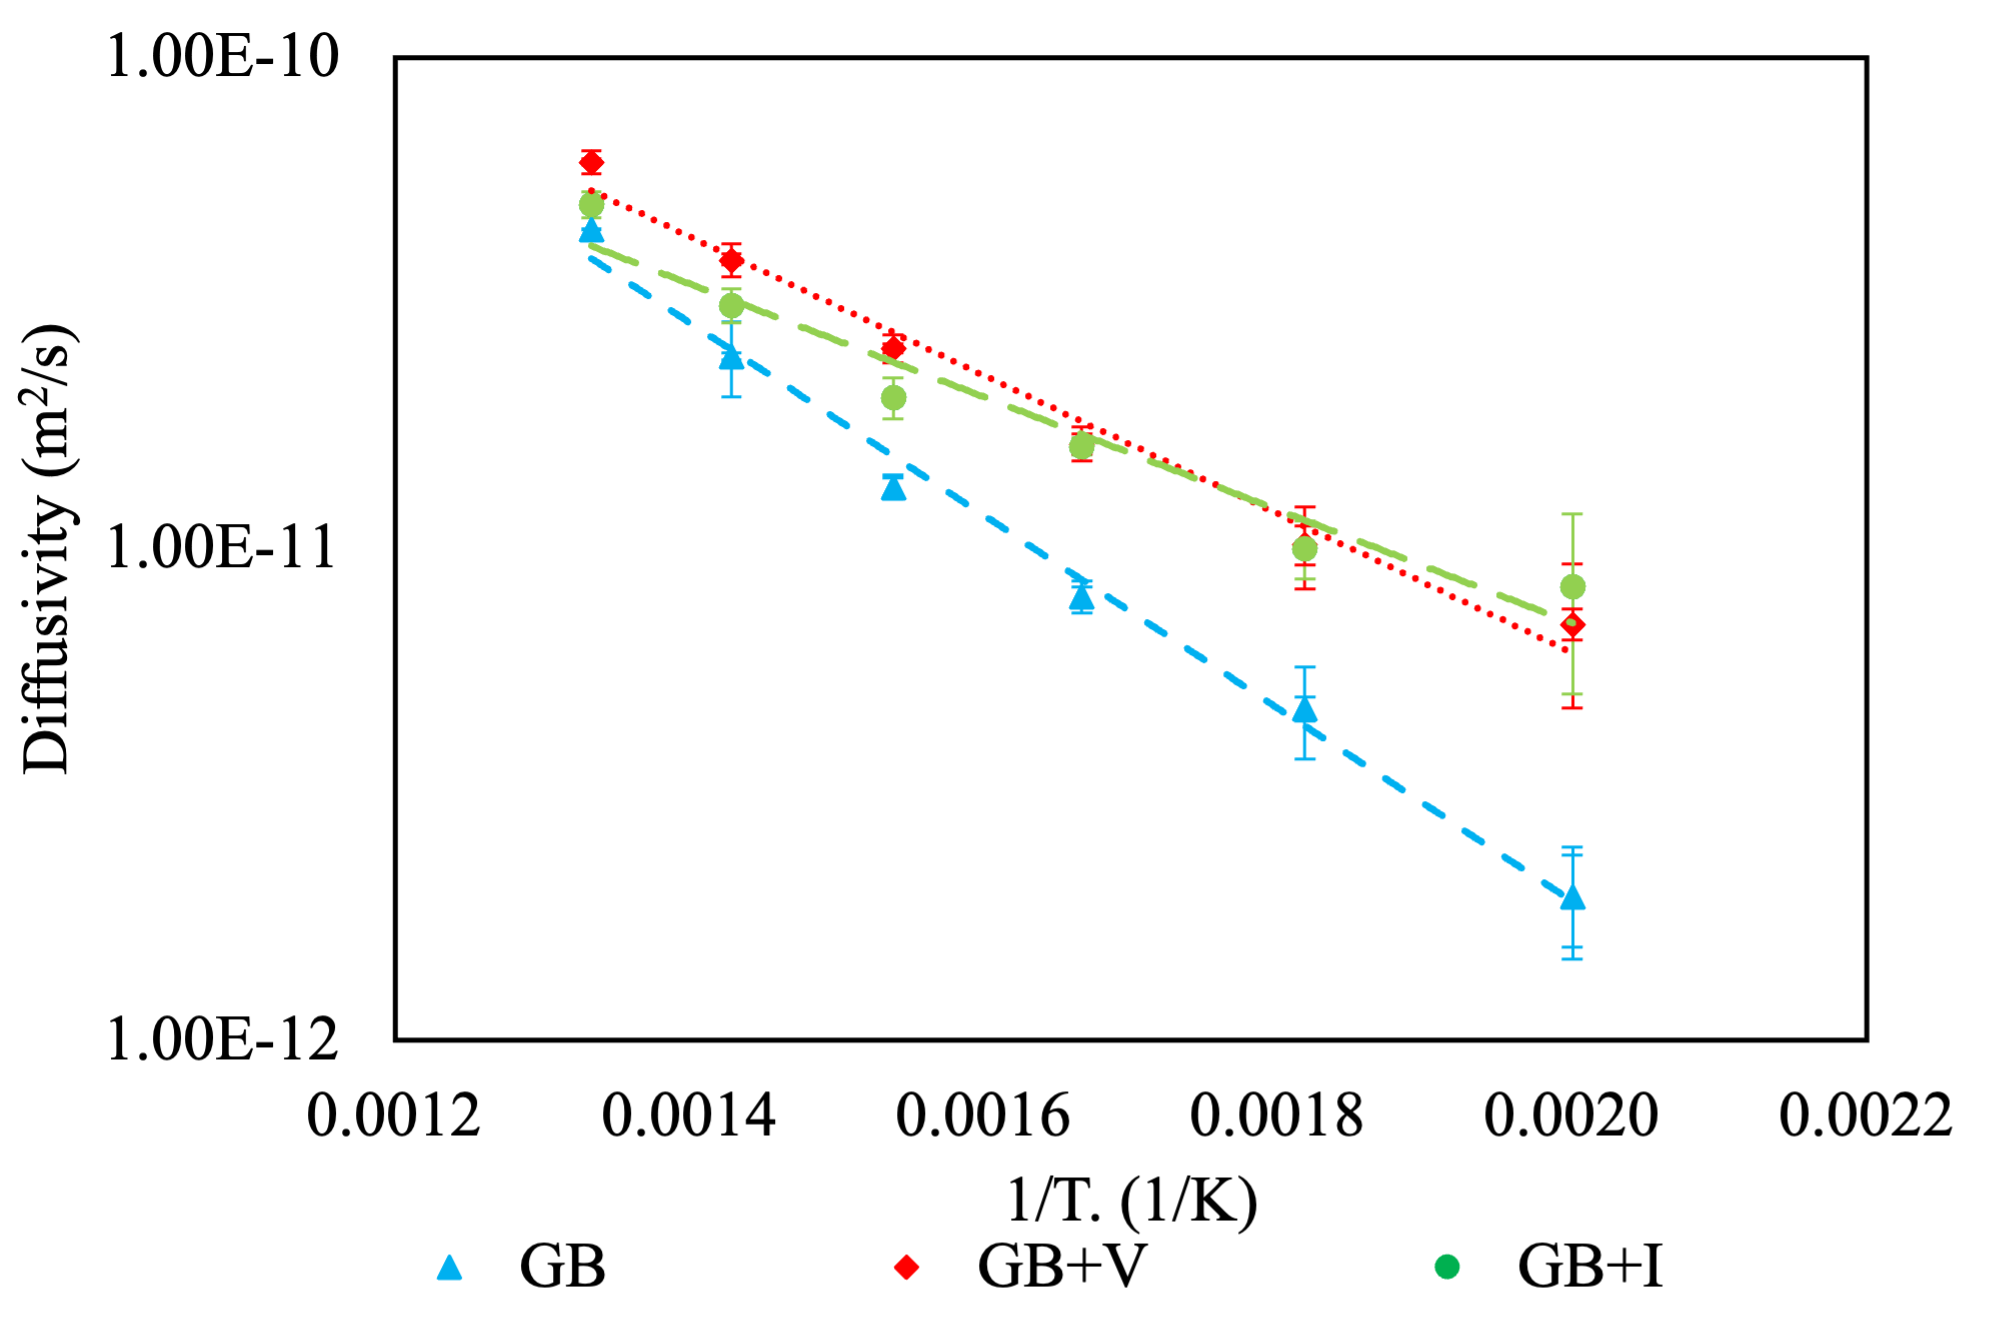
\includegraphics[width = 2.25in]{9_B2_diffusion.png}} 
\subfloat[]{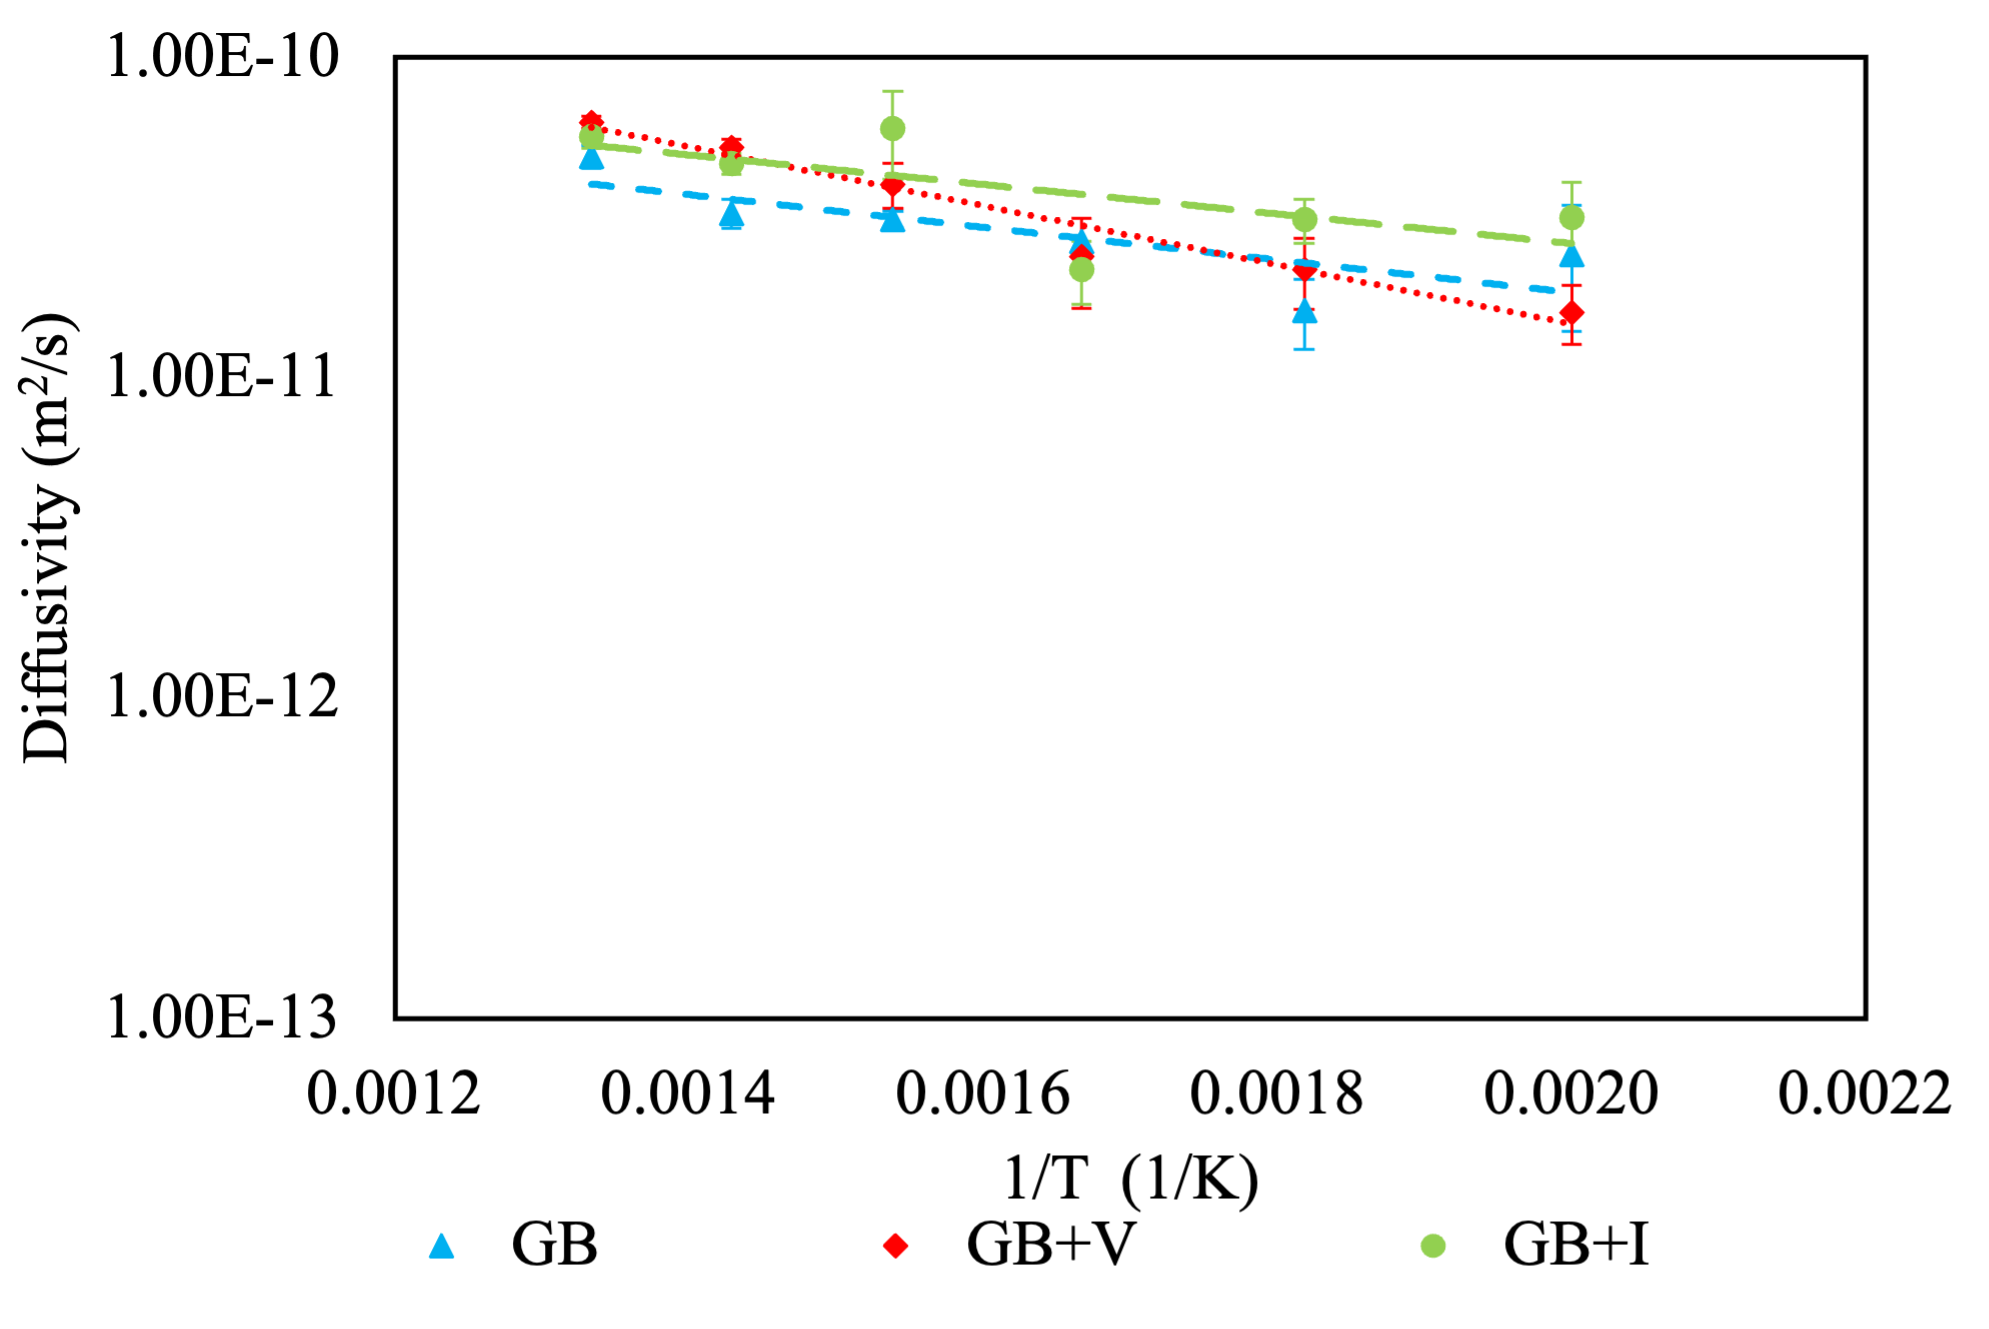
\includegraphics[width = 2.25in]{9_C2_diffusion.png}}\DIFaddendFL \\
\caption{Arrhenius plot of $\alpha$-U diffusion through high-energy grain boundaries (a) A2, (b) B2, and (c) C2. In the legend, GB+V denotes diffusion with an added vacancy, GB+I denotes diffusion with an added interstitial, and no additional label means diffusion through an as-constructed GB. Straight lines here represent the fitted Arrhenius equation. Here, the error bars represent one standard error.}
\label{fig:Dif_fit2}
\end{figure}

An additional diffusion path is formed along the tilt axis on the shear plane of the C2 GB to accommodate the pipe diffusion. Atoms at the GB follow this additional diffusion path and then diffuse via the pipe directions. As a result, the C2 GB shows the highest diffusivity among the high-energy GBs. At temperatures below 500 K, the C2 GB diffusion is 5.5 times higher than the A2 GB and 8.4 times higher than the B2 GB. This ratio decreases with increasing temperature, but diffusion in the C2 GB remains the most rapid. $\alpha$-U atoms diffuse slowest through the A2 GB among the three high-energy GBs considered in the current work. The C2 GB possesses the highest formation energy, so it has a more distorted structure which leads to it having the highest diffusivity. Typically, high-energy GBs provide an easier pathway for diffusion. For example, the Ag diffusion rate through a high-energy SiC GB is higher than via low-energy GBs \cite{SiC_HE}.

By inserting an interstitial within the GB interaction zone (GB+I), self-diffusion increases by, on average, 1.5 times. On the other hand, with the insertion of a vacancy, the diffusivity increases by an average of 1.45 times for temperatures greater than 600 K. The differences are considered statistically insignificant in all but the B2 case, which shows significant enhancement with the insertion of either defect at low temperatures. The C2 GB remains the fastest diffusion path, including the GB+I and GB+V conditions. 

Considering the equal probability of the three GB self-diffusion conditions (GB, GB+I, and GB+V), high-energy GBs show a higher average diffusivity compared to low-energy GBs. \Cref{fig:final} (a) portrays this feature. Furthermore, the weighted average technique is implemented based on the formation energies of the respective GBs (see \Cref{eq:weight}) to obtain the self-diffusivity of the specific GB type. The resulting GB diffusivity equations are shown in \Cref{eq:type,eq:type1,eq:type2}. By using this method, type C has the highest diffusivity over the entire temperature range, followed by type B, and finally type A. These results are shown in \Cref{fig:final} (b). %While the segregation of point defects in GBs is independent on grain boundary orientation, the average self-diffusion of the $\alpha$-U GBs depends on grain boundary orientation. 

\begin{equation}
\label{eq:type}
D_{GB,A} = 7.05 \times 10^{-10} \exp\left(\frac{-0.272}{k_{B} T}\right)
\end{equation}

\begin{equation}
\label{eq:type1}
D_{GB,B} = 7.92 \times 10^{-10} \exp\left(\frac{-0.248}{k_{B} T}\right)
\end{equation}

\begin{equation}
\label{eq:type2}
D_{GB,C} = 1.44 \times 10^{-10} \exp\left(\frac{-0.124}{k_{B} T}\right)
\end{equation}

\begin{figure}[h!]
\centering
\DIFdelbeginFL %DIFDELCMD < \subfloat[]{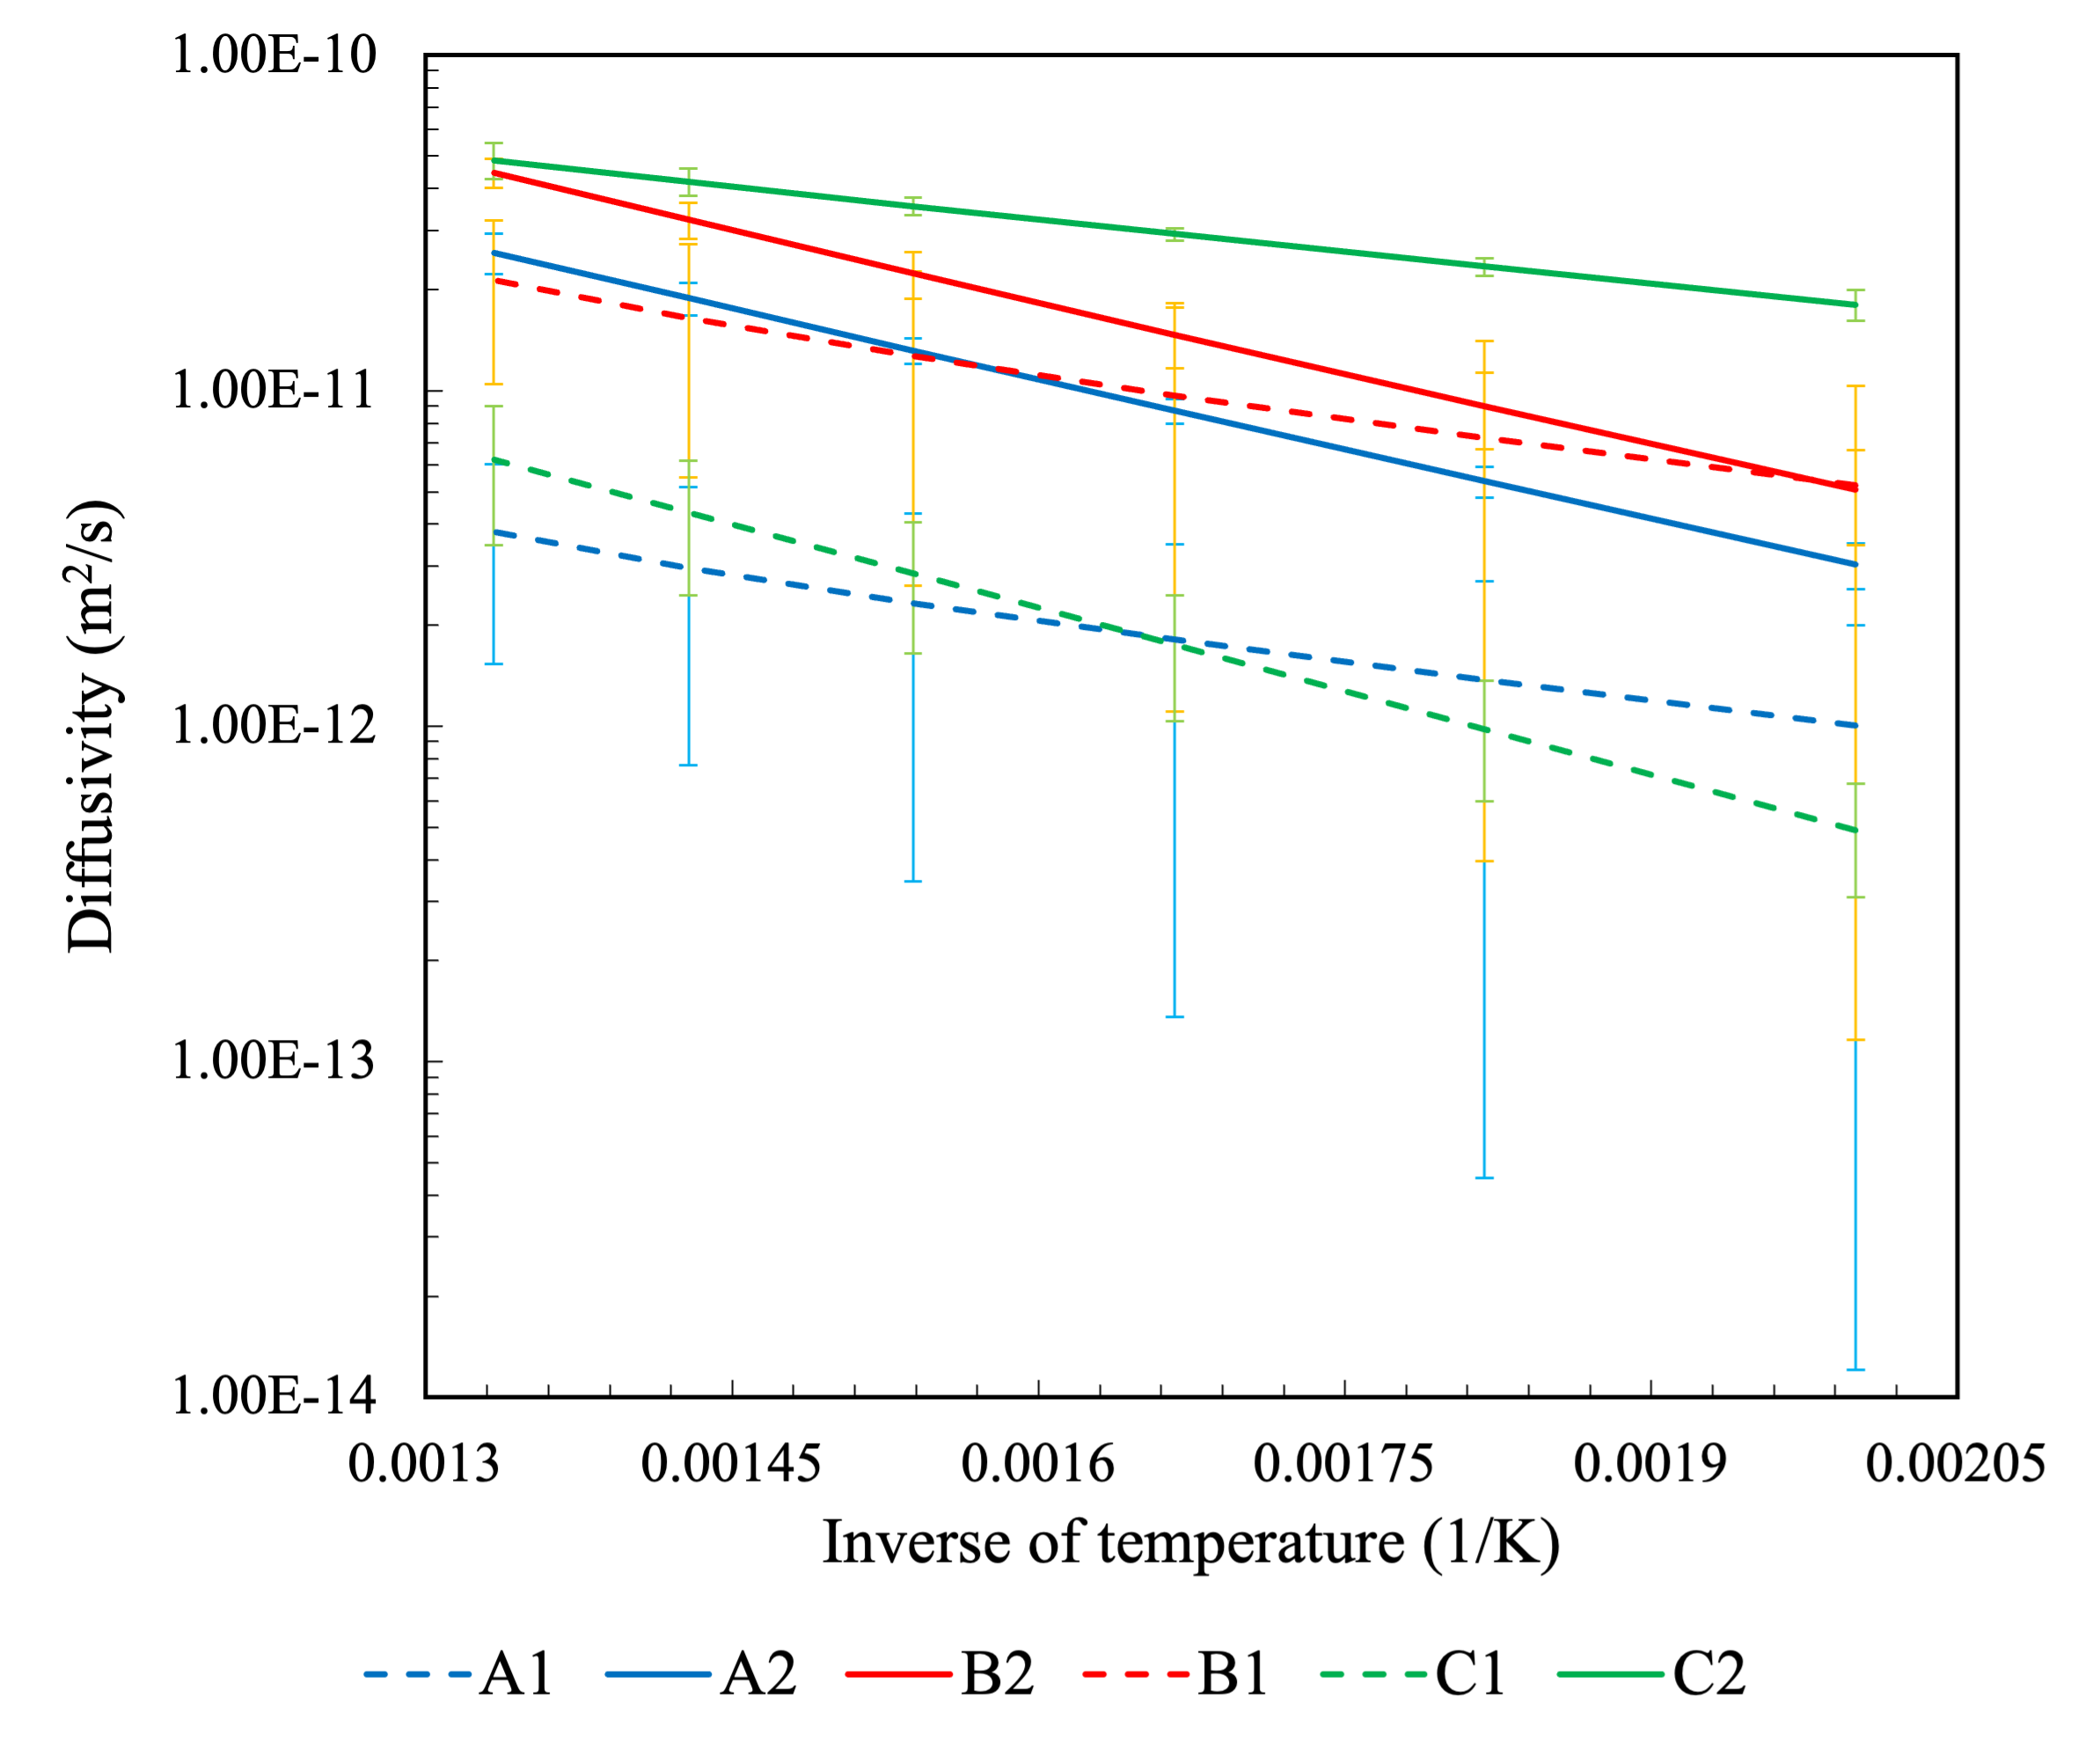
\includegraphics[width = 2.8in]{final2.png}}
%DIFDELCMD < %%%
%DIF < \subfloat[]{\includegraphics[width = 2.2in]{final.png}} 
%DIFDELCMD < \subfloat[]{\includegraphics[width = 2.8in]{final1.png}} 
%DIFDELCMD < %%%
\DIFdelendFL \DIFaddbeginFL \subfloat[]{\includegraphics[width = 2.8in]{10_final2.png}}
\subfloat[]{\includegraphics[width = 2.8in]{10_final1.png}} 
\DIFaddendFL \caption{Considering the equal probability of three GB self-diffusion conditions (GB, GB+V, GB+I) of all GBs studied, Arrhenius plot of (a) GB self-diffusivity of all GBs studied and (b) Arrhenius plot of weighted averaged diffusivity of the same type of GBs of $\alpha$-U based on their formation energy.}
%DIF < diffusivity of the same type of GBs of $\alpha$-U, and (c) weighted averaged diffusivity of the same type of GBs of $\alpha$-U is plotted over the temperature.}
\label{fig:final}
\end{figure}

The GB self-diffusion results are compared with interstitial, vacancy, and self-diffusion in bulk $\alpha$-U in \Cref{fig:Dif} \cite{WANG2023154289}. GB self-diffusion for all six studied GBs is 10${^7}$ to 10$^{13}$ times faster than the self-diffusion of the bulk system. The difference in GB diffusion to self-diffusion decreases with increasing temperature, which is expected. Assuming that the system is comprised mainly of low-energy GBs, we would expect that the GB diffusion would be approximately 7$\times$10$^{7}$ times the bulk diffusion at 750 K, which is considered a reasonable temperature for the region of the fuel slug which contains $\alpha$-U \cite{KIM200617}. High-energy GBs (A2, B2, and C2) have about 50\%\ higher diffusivity than the low-energy GBs. If we consider an equal probability of all GB types studied in this work, then the GB diffusion would be approximately 8$\times$10$^{11}$ times the bulk diffusion at 750 K. Regardless, GB diffusion is significantly faster than bulk diffusion and must be considered at reactor-relevant temperatures. 

\begin{figure}[h!]
\centering
\DIFdelbeginFL %DIFDELCMD < \subfloat[]{\includegraphics[height = 2.4in]{A_diffusion.png}}
%DIFDELCMD < \subfloat[]{\includegraphics[height = 2.4in]{B_diffusion.png}} 
%DIFDELCMD < \subfloat[]{\includegraphics[height = 2.4in]{C_diffusion.png}}%%%
\DIFdelendFL \DIFaddbeginFL \subfloat[]{\includegraphics[height = 2.4in]{11_A_diffusion.png}}
\subfloat[]{\includegraphics[height = 2.4in]{11_B_diffusion.png}} 
\subfloat[]{\includegraphics[height = 2.4in]{11_C_diffusion.png}}\DIFaddendFL \\
\caption{Diffusion through (a) type A, (b) type B, and (c) type C grain boundaries of $\alpha$-U as a function of the reciprocal temperature. In the legend, A2 (GB+V) denotes self-diffusion through the A2 grain boundary in the presence of a vacancy. Similarly, A2 (GB+I) denotes self-diffusion through the A2 grain boundary in the presence of an interstitial, and A2 (only GB) denotes self-diffusion through a pristine A2 grain boundary. Red lines denote the diffusivity of vacancies and interstitials in bulk $\alpha$-U. The black line shows the bulk self-diffusivity of $\alpha$-U atoms.}
\label{fig:Dif}
\end{figure}




Both the migration energy ($E_{\mathrm{m}}$) and the pre-exponential factor of the Arrhenius relation are the parameters of interest and can be determined from the diffusion coefficients displayed in the prior section. The determined $E_{\mathrm{m}}$ are displayed in \Cref{fig:Migra} and are also tabulated in the Appendix in \Cref{tab:migra} for all studied GBs and defect conditions. Similarly, pre-exponential constants are tabulated in the Appendix in \Cref{tab:pre} for all studied GBs and defect conditions. From \Cref{fig:Migra}, grain boundaries with added vacancies (GB+V) typically display higher $E_{\mathrm{m}}$ than other studied systems (GB or GB+I). The highest $E_{\mathrm{m}}$ was observed for the A1 GB, with a value of 0.626 $\pm$ 0.006 eV. Systems with added interstitials are generally equal to or lower in $E_{\mathrm{m}}$ than the systems with an added vacancy or no vacancy defects. The minimum $E_{\mathrm{m}}$ was observed for the C2 GB, with a value of 0.09 $\pm$ 0.02 eV. There is not a clear trend in $E_{\mathrm{m}}$ when comparing high-energy to low-energy GBs. 

\begin{figure}[h!]
\centering
\DIFdelbeginFL %DIFDELCMD < \includegraphics[width = 3in]{migration.png}%%%
\DIFdelendFL \DIFaddbeginFL \includegraphics[width = 3in]{12_migration.png}\DIFaddendFL \
\caption{Migration energy for grain boundary diffusion in the A1, A2, B1, B2, C1, and C2 grain boundaries in $\alpha$-U for three separate defect conditions. GB: no added defects, GB+I: added interstitial, GB+V: added vacancy. Error bars represent the maximum and minimum migration energy. Red and green horizontal lines represent migration energy for a vacancy and an interstitial through bulk $\alpha$-U \cite{WANG2023154289}, respectively.}
\label{fig:Migra}
\end{figure}

Prior molecular dynamics \cite{WANG2023154289} and density functional theory \cite{wirth2011} studies have found that the $E_{\mathrm{m}}$ for bulk interstitial diffusion is in the range of 0.2 - 0.4 eV, and the $E_{\mathrm{m}}$ for bulk vacancy diffusion is in the range of 0.3 - 0.4 eV, with specific directions exhibiting higher $E_{\mathrm{m}}$. \Cref{fig:Migra} shows that the magnitude of the $E_{\mathrm{m}}$ for GB diffusion varies from 0.1 eV to 0.6 eV, which is in line with these prior computational studies on $E_{\mathrm{m}}$ of point defects in the bulk, albeit with a slightly lower minimum value. Comparing the pre-factor for point defect diffusion to GB self-diffusion \cite{WANG2023154289}, the pre-factor obtained in this work is two to three orders of magnitude lower than for point defect diffusion. Thus, the difference in the formation energy of a defect species in the bulk versus at a grain boundary is the predominant factor in the accelerated GB diffusion compared to the bulk.


\subsection{Coble creep}

\par Utilizing the diffusion data obtained from the current work, diffusional creep along GBs, i.e., Coble creep \cite{coble} rate for $\alpha$-U is further computed. Coble creep is calculated for the six studied GBs utilizing the methodology of Cooper \cite{USi_diffusion} in which the Coble creep rate of a $\Sigma$530 tilt grain boundary of U$_\mathrm{3}$Si$_\mathrm{2}$ was studied using molecular dynamics. To calculate the Coble creep rate ($\dot{\epsilon}_{Coble,x,y}$) for an arbitrary stress ($\sigma$) and grain size (d), the GB diffusivity (D$_{GB}$) and GB width ($\delta$) are utilized and \Cref{eq:coble} is applied. 

\begin{equation}
\label{eq:coble}
\dot{\epsilon}_{Coble,x,y} =\frac{42 |\ohm_{x}| \pi (D )_{GB,y} \delta}{k_{B} T d^{3}} \sigma \\
\end{equation}

\noindent For the studied GBs and temperatures, the GB width is observed (see \cref{sec:comp2}) to be in the range between 1.5 nm to 2.0 nm. Thus, in the Coble creep equation, it is considered as 1.6 nm. $x$ denotes either an interstitial or a vacancy and $y$ denotes the GB (type A, type B, type C). Comparing the Coble creep rate of different types of GBs of $\alpha$-U, type C shows the maximum creep rate followed by type B and type A. At a temperature of 750 K, type B, and type C have 1.4 times and 2.4 times higher diffusional creep rates than type A. The weighted average GB diffusivity for each type of GB is considered in the Coble creep calculation. The defect volume for vacancy and interstitial is taken as the temperature-averaged value from Wang \textit{et al.} \cite{WANG2023154289}. The defect volume considered in the current work is 8.33$\times$10$^{-30}$ m$^\mathrm{3}$and 13.67$\times$10$^{-30}$ m$^\mathrm{3}$ for interstitial and vacancy, respectively. The creep rate is fitted using \Cref{eq:coble1} \cite{USi_diffusion}. 

\begin{equation}
\label{eq:coble1}
\dot{\epsilon}_{Coble,x,y} =\frac{\sigma}{ T d^{3}} A_{cr,x,y} \times \exp\left(\frac{-E_{cr,x,y}}{k_{B} T}\right)\\
\end{equation}
% 
The pre-factor $A_{cr,x,y}$ and the creep activation energy $E_{cr,x,y}$ for different GB types in \Cref{eq:coble1} are listed in the appendix in \Cref{tab:creep}. The creep rate for a given GB is given as a summation of the contribution from the vacancy and interstitial. The Coble creep rate in polycrystalline $\alpha$-U is nearly isotropic \cite{calhoun}. By taking the average creep rate from each type of GB, an estimate of the Coble creep rate of $\alpha$-U is made. Thus, the proposed Coble creep rate equation for $\alpha$-U is:

\begin{equation}
\label{eq:coble2}
\dot{\epsilon}_{Coble} =\frac{\sigma}{T d^{3}} 3.269 \times 10^{-22} \exp\left(\frac{-0.221}{k_{B} T}\right)
\end{equation}



\FloatBarrier

\section{Discussion}

In this section, discussions on the point defect interaction with grain boundary ($E_{\mathrm{s}}$, $l_{\mathrm{int}}$), grain boundary self-diffusion, and Coble creep are presented. The results are further compared with the results available in the literature. 

\subsection{Point Defect Interactions with Grain Boundaries}

\DIFaddbegin \par \DIFadd{Segregation energies ($E_{\mathrm{s}}$) at all temperatures for all studied GBs are plotted with respect to the corresponding  $E_{\mathrm{gb}}$  in \Cref{fig:SE_GB}. Data for interstitials and vacancies can be separately fitted by a linear function. The $E_{\mathrm{s}}$ increases with  $E_{\mathrm{gb}}$  at a rate of 2.99 eV per $J/m{^2}$ for interstitials and 2.92 eV per $J/m^2$ for vacancies. Though both of the point defect types have similar rates of increase, there is a threshold value in $E_{\mathrm{gb}}$ for vacancy segregation which is about 0.4 $J/m^2$. An MD study on $\alpha$-Fe for both tilt and twist GBs showed a linear relationship of point defect $E_{\mathrm{s}}$ with $E_{\mathrm{gb}}$ \cite{tschopp2012probing}, essentially confirming the results here, albeit in a different material and with different functional slopes. 
}

\begin{figure}[h!]
\centering
\includegraphics[width = 3in]{13_SE_GB.png}\\
\caption{\DIFaddFL{Segregation energy of point defects at GBs in $\alpha$-U at different studied temperatures plotted as a function of the corresponding $E_{\mathrm{gb}}$.}}
\label{fig:SE_GB}
\end{figure}

\DIFaddend To the authors' knowledge, there are no prior results on the point defect segregation energy \DIFaddbegin \DIFadd{($E_{\mathrm{s}}$) }\DIFaddend on GB are available for metallic U for comparison, but other metallic systems can be considered. For pure Cu, high-symmetry GBs at 300 K \cite{bai_cu_inter, bai_cu_gb_with_interstitial_inter} have a  $E_{\mathrm{gb}}$  between 0.31 J/m${^2}$ to 0.89 J/m${^2}$ and the segregation energy for interstitials and vacancies is calculated within the range of 1.6 eV to 3 eV and 0.2 eV to 1.1 eV \cite{bai_cu_inter}, respectively. At 300 K, the  $E_{\mathrm{gb}}$  of the studied GBs in $\alpha$-U is between 0.22 J/m${^2}$ to 0.86 J/m${^2}$ \cite{MAHBUBA2021153072}, while the segregation energy varies between 0.42 eV to 2.5 eV for interstitials and 0 eV to 1.57 eV for vacancies. Thus, for GBs of similar energies, the $E_{\mathrm{s}}$ of vacancies is similar for fcc Cu and $\alpha$-U, but interstitials in $\alpha$-U exhibit somewhat lower $E_{\mathrm{s}}$. For Nb, the $E_{\mathrm{s}}$ of a vacancy around four STGBs was calculated to be between 0.1 eV to 2.2 eV \cite{Popov2022}. Moreover, a lower segregation energy for low-energy GBs is observed for Nb. An MD study on Mo symmetric tilt GBs showed a higher $E_{\mathrm{s}}$ for interstitials than vacancies\cite{Novoselov2014}. Another study examining defect segregation in U$_3$Si$_2$ was performed and can be utilized for comparison to this work \cite{beelerUSi}. Uranium vacancies and interstitials show a lower $E_{\mathrm{s}}$ in U$_\mathrm{3}$Si$_\mathrm{2}$ (vacancies and interstitials both approximately 1.3 eV) than in $\alpha$-U symmetric tilt GBs. 

Like the $E_{\mathrm{s}}$, interaction length ($l_{\mathrm{int}}$) is compared with other metallic systems because of the unavailability of results on $\alpha$-U. Comparing the $l_{\mathrm{int}}$ results obtained from the current work with pure Cu high-symmetry GBs at 300 K \cite{bai_cu_inter, bai_cu_gb_with_interstitial_inter}, similar behavior is observed, where the  $l_{\mathrm{int}}$ for an interstitial and a vacancy is calculated within the range of 9.2 - 30.2~{\AA} and 2 - 8~{\AA} \cite{bai_cu_inter}, respectively. In the current work, the  $l_{\mathrm{int}}$ varies from 6.1 - 21.0~{\AA} and 11.5 - 15.1~{\AA} for an interstitial and a vacancy, respectively, at 300 K. These comparisons show that vacancies in $\alpha$-U have a larger  $l_{\mathrm{int}}$ than Cu GBs, while the  $l_{\mathrm{int}}$ for interstitials is similar to that of Cu. The low-temperature phase of Fe ($\alpha$-Fe) has a minimum  $l_{\mathrm{int}}$ length of 7 {\AA} for vacancies and 8 {\AA} for interstitials \cite{tschopp2012probing}, indicating a minimally longer $l_{\mathrm{int}}$ for interstitials than in $\alpha$-U. Similar to the $E_{\mathrm{s}}$, the $l_{\mathrm{int}}$ in U$_\mathrm{3}$Si$_\mathrm{2}$ of a vacancy and an interstitial is smaller than in $\alpha$-U GBs (only 5~{\AA} in U$_3$Si$_2$). \cite{beeler2019}, indicating less interaction of defects with GBs in U$_3$Si$_2$. 


\subsection{Diffusion along Grain Boundaries}

\par There is no experimental or computational data available for a comparison of the GB diffusion in the $\alpha$-U system, and only limited data is available for comparison in other related systems. If we extrapolate the diffusivity data available in the literature for intermetallic U$_\mathrm{3}$Si$_\mathrm{2}$ fuel to a lower temperature range (750 K to 500 K), it is observed that diffusion through $\alpha$-U GBs is several orders of magnitude higher than the diffusion through U$_\mathrm{3}$Si$_\mathrm{2}$ GBs. Conversely, GB diffusion of nanocrystalline $\alpha$-Fe based on molecular dynamics calculation shows higher diffusivity \cite{MOHAMMADZADEH201756} compared to the current work. The self-diffusivity of Cu high-energy symmetric tilt GBs utilizing kMC atomistic simulations are in a similar order of magnitude as the $\alpha$-U GBs \cite{Suzuki2003}. Compared with other pure metals in \Cref{fig:diff_comp}, including silver, lead, tin, zinc, and cadmium, $\alpha$-U GBs show the lowest diffusivity \cite{diffusion_compare}. Grain boundary diffusivity data for these metals are available from experimental studies as a function of GB width ($\delta$) and temperature. In \Cref{fig:diff_comp}, the Arrhenius relationship is shown between GB width ($\delta$) times diffusivity (D$_\mathrm{GB}$) as a function of the inverse of the temperature. Fitting parameters for the Arrhenius relationship between $\delta$D$_\mathrm{GB}$ and the inverse of temperature for $\alpha$-U are listed in \Cref{tab:widthanddiff}. Another molecular dynamics study on a nanocrystalline Cu-Nb alloy found its GB self-diffusivity to be several orders lower in magnitude \cite{cu_nb} than that of $\alpha$-U GBs. Considering that GB diffusion in $\alpha$-U is lower or higher than these reported pure metals and U$_3$Si$_2$, and significantly faster than lattice diffusion, the predicted results presented here are reasonable. Experimental efforts to provide additional data for comparison are necessary for further validation. 

\begin{figure}[h!]
\centering
\DIFdelbeginFL %DIFDELCMD < \subfloat[]{\includegraphics[width = 0.45\textwidth]{1.png}}
%DIFDELCMD < \subfloat[]{\includegraphics[width = 0.45\textwidth]{3.png}}%%%
\DIFdelendFL \DIFaddbeginFL \subfloat[]{\includegraphics[width = 0.45\textwidth]{14_1_2.png}}
\subfloat[]{\includegraphics[width = 0.45\textwidth]{14_3.png}}\DIFaddendFL \\
\caption{(a) The Arrhenius relationship between the GB width ($\delta$) multiplied by diffusivity vs. the inverse temperature for Sn, Cd, Pb, Zn, Ag, $\alpha$-Fe, and Co GBs (\cite{diffusion_compare}) experimental results along with kMC-based results for Cu and Nb GBs \cite{cu_nb}. These values are compared with the average GB self-diffusivity of $\alpha$-U as a function of GB width ($\delta$) and temperature;(b) The Arrhenius relationship between the GB self diffusivity vs. the inverse temperature for Cu $\sum$5(210), Cu $\sum$13(341) \cite{Suzuki2003}, U atom in U$_\mathrm{3}$Si$_\mathrm{2}$ \cite{COOPER2021153129}, Au GBs \cite{diffusion_compare}, along with $\alpha$-U type A and type C GBs. Data from the literature are extrapolated to the studied temperature range.}
\label{fig:diff_comp}
\end{figure}


The results for migration energies in \Cref{fig:Migra} also generally compare well to prior studies on Cu. The $E_{\mathrm{m}}$ of Cu diffusivity through symmetric tilt GBs is reported as 0.83 eV \cite{AginCu}.
%which is two to five times higher than that of $\alpha$-U GBs. 
In an article by Suzuki \cite{Suzuki2003} utilizing kinetic Monte Carlo (kMC), the $E_{\mathrm{m}}$ of the diffusivity either parallel or perpendicular to the GBs of Cu is reported between 0.51 eV to 2.1 eV \cite{Suzuki2003}. In another molecular dynamics simulation work on the Cu-Nb alloy system, the $E_{\mathrm{m}}$ for Cu is calculated as 0.71 eV and the $E_{\mathrm{m}}$ for Nb is reported as 0.91 eV\cite{cu_nb}. A separate MD study on a set of STGBs in Nb showed the $E_{\mathrm{m}}$ of the GB self-diffusivity is on the order of 2 eV \cite{Popov2022}. The migration energy for GB self-diffusion of nanocrystalline $\alpha$-Fe \cite{MOHAMMADZADEH201756} is calculated as 0.101 eV using MD. Thus, the findings are comparable for $E_{\mathrm{m}}$ comparisons between different pure metals and $\alpha$-U GBs.
%Moreover, Mo also shows higher migration energy for GB self diffusivity which is reported as 2.5 - 2.8 eV via MD study \cite{Popov2022}. 

The compensation law, or Meyer-Neldel rule (MNR), is a fundamental property in many thermally activated processes that follow the Arrhenius law. This law represents a linear relationship between the logarithmic of the pre-exponential factor and the $E_{\mathrm{m}}$. In the case of interfacial diffusion of pure metallic systems via MD simulations, the compensation law is observed to be valid for Ag, Au, Pd, and Ni high-symmetry surfaces \cite{compansation}, as well as for Ni GB self-diffusion \cite{Mendelev2005}. For the studied GBs of $\alpha$-U, as the $E_{\mathrm{m}}$ increases, the GB self-diffusion pre-exponential constant also increases logarithmically, as shown in see \Cref{fig:compan}. Thus, we predict that for STGBs of $\alpha$-U, GBs with a larger $E_{\mathrm{m}}$ for diffusion compensate for the difficulties in diffusion by increasing the pre-exponential factor (e.g., the attempt frequency). No experimental evidence of the compensation law in $\alpha$-U GB self-diffusion has been reported to the authors' knowledge.

\begin{figure}[h!]
\centering
\DIFdelbeginFL %DIFDELCMD < \subfloat[]{\includegraphics[width = 0.5\textwidth]{compensation.png}}%%%
\DIFdelendFL \DIFaddbeginFL \subfloat[]{\includegraphics[width = 0.5\textwidth]{15_compensation.png}}\DIFaddendFL \\
\caption{Natural logarithm of the pre-exponential factor versus migration energy (Meyer-Neldel rule) for grain boundary self-diffusion of $\alpha$-U.}
\label{fig:compan}
\end{figure}

\subsection{Coble creep}

Within the operating temperature and pressure of metallic fuel, Coble creep in $\alpha$-U is one of the most dominant deformation mechanism. To get an estimate of what will be Coble creep rate in the actual reactor condition, Coble creep rate is calculated. For the operating conditions of metallic fuel \cite{recent_review} with a temperature ranging between 500 K to 750 K, gas/plenum pressure of 5 MPa, and average grain size of 0.55 $\mu$m \ (according to the TEM analysis of the irradiated sample C from Di Lemma \cite{DILEMMA2020152467}), the Coble creep rate of $\alpha$-U is calculated to be 8.06 $\times$ 10$^{-2}$ s$^{-1}$ to 2.22 $\times$ 10$^{-1}$ s$^{-1}$. The typical grain size in metallic UZr fuel is 10-20 $\mu$m \cite{osti_1469797}; for this grain size under similar pressure, the Coble creep of $\alpha$-U is estimated as 1.34 $\times$ 10$^{-5}$ s$^{-1}$ to 1.68 $\times$ 10$^{-6}$ s$^{-1}$. Other historic experimental data \cite{ROBINSON1973293} from compression tests on $\alpha$-U creep show a steady-state creep rate in the order of 10$^{-2}$ and 10$^{-6}$, but the creep mechanism is not Coble creep, as the normal stress exponent is between 4 to 6, implying dislocation climb. 

Similar pressure, temperature, and grain size are considered to compare Coble creep results with other uranium-based systems. The diffusional creep rate of $\alpha$-U GBs is significantly higher than that of U$_\mathrm{3}$Si$_\mathrm{2}$ (approximately 10$^{5}$ time at 750 K). For U$_\mathrm{3}$Si$_\mathrm{2}$, the Coble creep rate is limited by the Si defects, but in our study, there are no extrinsic species to be considered. Moreover, in U$_\mathrm{3}$Si$_\mathrm{2}$ \cite{COOPER2021153129} the GB width is considered to be 1 nm, and the studied temperature range is 1200 K to 1600 K. In order to compare results, the data must be extrapolated to lower temperatures by assuming that the diffusion parameters will remain the same at lower temperatures, which may not be the case. Although both materials are uranium-based and a similar methodology is utilized, because of the alloying of U with Si, the Coble creep rate is drastically decreased. Comparing the activation energy for the diffusional creep rate of $\alpha$-U with polycrystalline UO$_\mathrm{2}$ \cite{DESAI20084489}, $\alpha$-U has approximately an order of magnitude lower activation energy (0.221 eV) than UO$_\mathrm{2}$ (3.86 eV \cite{DESAI20084489}). The activation energy for GB diffusional creep of polycrystalline Pd is calculated as 0.61 eV \cite{YAMAKOV200261_Pd_creep}, which is in the similar order of magnitude of $\alpha$-U. In the case of UO$_2$, the Coble creep rate is limited by the diffusion of U atoms. Under a stress of 5 MPa and with a grain size of 15 $\mu$m, the diffusional creep rate of $\alpha$-U and U$_\mathrm{3}$Si$_\mathrm{2}$ is approximately 10$^{11}$ and 10$^{5}$ higher, respectively, than UO$_\mathrm{2}$ at 750 K.  


\section{Conclusion}
The interaction of interstitials and vacancies with six symmetric tilt grain boundaries in $\alpha$-U and self-diffusion along those grain boundaries have been explored utilizing molecular dynamics simulations. $\alpha$-U GBs are classified based on the shear plane orientation: type A, type B, and type C, with two GBs from each of the types considered in the current study. We find that GBs of $\alpha$-U are biased sinks for interstitials compared to vacancies. The segregation energies of both point defect types follow an increasing linear trend with the $E_{\mathrm{gb}}$, in that segregation is preferable at higher energy grain boundaries. Two low-energy GBs show no interaction with vacancies. Both the interaction length and the segregation energy are effectively temperature-independent over the studied temperature range. %Average GB interaction properties with point defect for three different type GBs are calculated using both simple averaging and weighted averaging technique. Neither segregation energy nor the interaction length are function of temperature. 
The self-diffusivity of GBs was calculated as a function of temperature, including systems with an added defect. High-energy GBs show approximately four times faster diffusivity compared to low-energy GBs, and the presence of point defects at the GB slightly enhances the diffusivity for high-energy GBs. The GB diffusivity of $\alpha$-U is lower than that of other pure metals while it is higher than that of U$_3$Si$_2$, which is the only other metallic U compound for which there is data against which to compare. Finally, the results from the self-diffusivity were used to calculate the Coble creep equation for $\alpha$-U for the first time.

This study provided the first investigation of point defect interactions with grain boundaries and is the first study of grain boundary diffusion in metallic pure U. Results from this study can be implemented in kinetic Monte Carlo, rate-theory, and phase-field modeling methodologies to develop and improve mechanistic fuel performance modeling of metallic-fueled advanced nuclear reactors, and further elucidate the fundamental irradiation response behavior of $\alpha$-U. 

\section{Acknowledgement}
Work supported through the INL Laboratory Directed Research and Development (LDRD) Program under DOE Idaho Operations Office Contract DE-AC07-05ID14517. This manuscript has been authored by Battelle Energy Alliance, LLC with the U.S. Department of Energy. The publisher, by accepting the article for publication, acknowledges that the U.S. Government retains a nonexclusive, paid-up, irrevocable, worldwide license to publish or reproduce the published form of this manuscript, or allow others to do so, for U.S. Government purposes. This research made use of the resources of the High Performance Computing Center at Idaho National Laboratory, which is supported by the Office of Nuclear Energy of the U.S. Department of Energy and the Nuclear Science User Facilities.


 \newpage

\section{Appendix}
\setcounter{figure}{0}
\setcounter{table}{0}
\renewcommand{\thefigure}{A\arabic{figure}}
\renewcommand{\thetable}{A\arabic{table}}
\setlength{\arrayrulewidth}{.5mm}
\setlength{\tabcolsep}{12pt}
\renewcommand{\arraystretch}{1.0}

The formation energy of an interstitial as a function of distance from a GB is shown in \Cref{fig:Seg_inter} for all six types of grain boundaries at 300, 400, and 600 K.

\begin{figure}[h!]
\centering
\subfloat[]{\includegraphics[width = 2.0in]{A_300_Inter.png}}
\subfloat[]{\includegraphics[width = 2.0in]{B_300_Inter.png}} \subfloat[]{\includegraphics[width = 2.0in]{C_300_Inter.png}}\\
\subfloat[]{\includegraphics[width = 2.0in]{A_400_Inter.png}}
\subfloat[]{\includegraphics[width = 2.0in]{B_400_Inter.png}}
\subfloat[]{\includegraphics[width = 2.0in]{C_400_Inter.png}}\\
\subfloat[]{\includegraphics[width = 2.0in]{A_600_Inter.png}}
\subfloat[]{\includegraphics[width = 2.0in]{B_600_Inter.png}}
\subfloat[]{\includegraphics[width = 2.0in]{C_600_Inter.png}}
\caption{Average formation energy of an interstitial at different temperatures as a function of fractional distance from type A ((a) 300 K, (d) 400 K, (g) 600 K), type B ((b) 300 K, (e) 400 K, (h) 600 K), and type C ((c) 300 K, (f) 400 K, (i) 600 K) grain boundaries. The red line shows the formation energy of an interstitial in pristine, bulk $\alpha$-U. The error bars here show twice the standard error.}
\label{fig:Seg_inter}
\end{figure}
\newpage

The formation energy of a vacancy as a function of distance from a GB is shown in \Cref{fig:Seg_vacancy} for all six types of grain boundaries at 300, 400, and 600 K.

\begin{figure}[h!]
\centering
\subfloat[]{\includegraphics[width = 2.0in]{A_300_Vacan.png}} 
\subfloat[]{\includegraphics[width = 2.0in]{B_300_Vacan.png}} 
\subfloat[]{\includegraphics[width = 2.0in]{C_300_Vacan.png}}\\
\subfloat[]{\includegraphics[width = 2.0in]{A_400_Vacan.png}} 
\subfloat[]{\includegraphics[width = 2.0in]{B_400_Vacan.png}} 
\subfloat[]{\includegraphics[width = 2.0in]{C_400_Vacan.png}}\\
\subfloat[]{\includegraphics[width = 2.0in]{A_600_Vacan.png}} 
\subfloat[]{\includegraphics[width = 2.0in]{B_600_Vacan.png}}
\subfloat[]{\includegraphics[width = 2.0in]{C_600_Vacan.png}}
\caption{ Average formation energy ($E_{\mathrm{f}}$) of a vacancy at different temperatures as a function of fractional distance from type A ((a) 300 K, (d) 400 K, (g) 600 K), type B ((b) 300 K, (e) 400 K, (h) 600 K), and type C ((c) 300 K, (f) 400 K, (i) 600 K) grain boundaries. The red line shows the formation energy of vacancy at pristine, bulk $\alpha$-U. The error bars show twice the standard error.}
\label{fig:Seg_vacancy}
\end{figure}
\newpage


\FloatBarrier

The migration energies along and the pre-exponential constant determined from diffusion along the grain boundaries for all six grain boundaries in defect-free and defected conditions are shown in \Cref{tab:migra} and \Cref{tab:pre}, respectively. 

{\footnotesize
\begin{table}[h!]
    \centering
    \caption{Calculated migration energy of the Arrhenius fit of self-diffusion of the six studied GBs of $\alpha$-U, each for three different conditions. Condition GB indicates that only the GB was simulated, GB+V denotes the GB with the presence of a vacancy, and GB+I denotes the GB with the presence of an interstitial. Migration energies listed here are plotted in \Cref{fig:Migra}. \label{tab:migra}}
\begin{tabular}{|c|c|c|c|}
\hline
\multicolumn{1}{|c}{Grain boundary}
& \multicolumn{3}{|c|}{Migration energy (eV) for different for different diffusion conditions} \\
\hline
 & GB & GB+V & GB+I \\
\hline
A1 &  & 0.62 & 0.147 \\
A2 & 0.258 & 0.432 & 0.253 \\
B1 &  & 0.61 & 0.184 \\
B2 & 0.421 & 0.321 & 0.276 \\
C1 &  & 0.348 & 0.353 \\
C2 & 0.159 & 0.214 & 0.117 \\
\hline
\end{tabular}
\end{table}

\begin{table}[h!]
    \centering
    \caption{Calculated pre-exponential constants of the Arrhenius fits of self-diffusion for the six studied GBs of $\alpha$-U, each for three different conditions. Condition GB denotes only the GB, GB+V denotes the GB with the presence of a vacancy, and GB+I denotes the GB with the presence of an interstitial.\label{tab:pre}}
    \begin{tabular}{|c|c|c|c|}
   \hline
\multicolumn{1}{|c}{Grain boundary}
& \multicolumn{3}{|c|}{ Pre-exponent constant (m$^3$/s) for different diffusion conditions} \\
\hline
 & GB & GB+V & GB+I \\
\hline
A1 &  & 1.6E-8 & 5.51E-11 \\
A2 & 1E-9 & 2.6E-8 & 1.2E-9 \\
B1 &  & 1.04E-7 & 4E-10 \\
B2 & 2.6E-8 & 8E-9 & 2E-9 \\
C1 &  & 6E-10 & 2E-9 \\
C2 & 4E-10 & 1.6E-9 & 2E-10 \\
\hline
    \end{tabular}
\end{table}
}

The Arrhenius fitting parameters for the grain boundary width times the grain boundary diffusion coefficient, $\delta$D$_\mathrm{GB}$, of three types of GBs in $\alpha$-U are shown in \Cref{tab:widthanddiff}.

\begin{table}[h!]
\centering
\caption{ Fitting parameters for Arrhenius relationship between $\delta$D$_\mathrm{GB}$ and inverse of temperature for three types of $\alpha$-U GBs. \label{tab:widthanddiff}}
\begin{tabular}{|c|c|c|}
\hline
\multicolumn{1}{|c}{Grain boundary}
& \multicolumn{1}{|c}{Migration energy (eV) } & \multicolumn{1}{c|}{Pre-factor (m$^{3}$s$^{-1}$) } \\
\hline

A & 0.302 & 2.77 $\times$ 10$^{-8}$ \\
B & 0.357 & 6.61 $\times$ 10$^{-8}$ \\
C & 0.213 & 1.77 $\times$ 10$^{-8}$ \\

\hline
\end{tabular}
\end{table}


The Arrhenius fitting parameters for Coble creep for the three types of GBs in $\alpha$-U are shown in \Cref{tab:creep}.
\begin{table}[h!]
\centering
\caption{Calculated activation energy of Coble creep and pre-factor as per \Cref{eq:coble1} of the three types of GBs of $\alpha$-U. Weighted average self-diffusion through each of the three types of grain boundaries is considered here. \label{tab:creep}}
\begin{tabular}{|c|c|c|}
\hline
\multicolumn{1}{|c}{Grain boundary}
& \multicolumn{1}{|c}{Creep activation energy (eV) } & \multicolumn{1}{c|}{Pre-factor (s$^{-1}$/($\frac{Pa}{m^3}$)) } \\
\hline

A & 0.272 & 2.69 $\times$ 10$^{-22}$ \\
B & 0.248 & 2.84 $\times$ 10$^{-22}$ \\
C & 0.124 & 5.16 $\times$ 10$^{-23}$ \\

\hline
\end{tabular}
\end{table}


\setlength{\arrayrulewidth}{.5mm}
\setlength{\tabcolsep}{12pt}
\renewcommand{\arraystretch}{1.0}



\newpage
\bibliography{MARMOT2.bib}
\bibliographystyle{elsarticle-num}

\end{document}
